\documentclass[12pt]{gshs_beamer_class}
% beamer ver2.0의 수정 사항
% 1. 기존 붉은색 이외에 녹색과 푸른색의 beamer도 제작 가능함 (색 변조한 학교 아이콘 ./logo 폴더에 탑재)
% 2. 수식 및 소스 코드 폰트 변경 부분 추가
% 3. 타이틀 페이지의 학교 아이콘을 벡터 이미지로 수정 및 크기 조정

%%%%%%%%%% *** Packages %%%%%%%%%%
%%%% 1) Following packages are included in the *.cls file:
%\usepackage{ifthen}
%\usepackage{xcolor}
%\usepackage{amssymb,amsmath,graphicx}
%\usepackage{etoolbox}
%\usepackage[hangul]{kotex}
%\usepackage{tikz}
%\usepackage{listings}

%%%% 2) Additional packages
\usepackage{framed}
\usepackage{array}
\usepackage{siunitx}
\usepackage{lipsum}
\usepackage{bookmark}


%\newtheorem{Qe}[defn]{Theorem}

%%%%%%%%%%%%%%%%%%%%%%%
%%% Question layout %%%
%%%%%%%%%%%%%%%%%%%%%%%
%\newenvironment{Q}
%{\color{red}\textbf{Q)}
%	\color{blue}$\rm{CO_2}{@Q}
%	\color{black}
%} 

%%%%%%%%%% *** Beamer Style Settings %%%%%%%%%%
%%%% 1) Theme Color
\themecolor{blue} %red, green, blue

%%%% 2) Equations Font Setter
% rm: classical LaTeX math font
% sf: cleaner font
\equationfont{rm} %rm, sf

%%%% 3) Listing (Source Code) Font Setter
% If you want to use typewriter font in listing environments, please delete the command below.
\usepackage{inconsolata}

%%%% 4) ToC Auto Producer
% ToC frame is added at the beginning of every section.
% If you want a title at ToC frames, please write the frametitle after 'begin frame.'
\AtBeginSection[]
{
	\begin{frame}{}
		\tableofcontents[currentsection]
	\end{frame}
}


%%%% 5) Line Strecth Setter
\renewcommand{\baselinestretch}{1.1}


%%%% 6) question and solution for student
\newcommand{\questionset}{\footnotesize\color{red}\textbf{Q)}\color{blue}}
\newcommand{\solutionset}{\newline\scriptsize\color{black!0}}

%%% 학생용을 출력할 경우 아래 줄 맨 앞에 % 표시를 추가하시오.
\renewcommand{\solutionset}{\pause\newline\scriptsize\color{black!70}}


%%%%%%%%%% *** The Title %%%%%%%%%%
\subtitle[]{대기과학 및 실험 (2022)}
\author[]{박 기 현 (Kiehyun.Park@gmail.com)}
\institute[]{과학영재학교 경기과학고등학교}
\date[]{\today}

%%\def\bookfile#1{\gdef\@bookfile{#1}}
%%\bookfile{../ref/The Atmosphere_an introduction to meteorology_Frederick K. Lutgens, Edward J. Tarbuck[13ed](2016).pdf}

%%%% pdf 책 파일의 경로
\newcommand{\bookfile}{../ref/The Atmosphere_an introduction to meteorology_Frederick K. Lutgens, Edward J. Tarbuck[13ed](2016).pdf}


%%%%%%%%%% *** The Body %%%%%%%%%%
\begin{document}\small

	%\setbeamertemplate{sidebar left}[sidebar theme] %sidebar
	%%%%%%%%%%%%%%%%%%%%%%%%%%%%%%%%%%%%%%%%%%%%%%%%%%%%%%%%
	%%%% Main Document 
	%%%% 컴파일 하고자 하는 챕터 앞의 %를 지우세요.
	%%%%%%%%%%%%%%%%%%%%%%%%%%%%%%%%%%%%%%%%%%%%%%%%%%%%%%%%
	
	%\include{sub/chap-{\chapNo}}
	%%%%%%%%%%% *** The Title %%%%%%%%%%
\title[]{대기에 대한 소개\\\small{제1장}}

\begin{frame}[plain] %title page
	\titlepage
\end{frame}


\begin{frame}[plain] %title page
	\ccpage
\end{frame}


	
\section{대기에 대한 포커스}

\begin{frame}[t]{극한 일기의 발생}
	\begin{tabular}{ll}
		\begin{minipage}[t]{0.50\textwidth}\	
			\begin{figure}[t]
				\includegraphics[trim=0 0 360 520, clip, page=35, width=\textwidth]
				{\bookfile}
			\end{figure}
		\end{minipage}	
		&
		\begin{minipage}[t]{0.45\textwidth}
			\begin{itemize}
				\item 날씨는 매일 뉴스에 나오는 일상의 한 부분
				\item 기록적인 기상현상의 발생 강도와 빈도가 증가하고 있음
			\end{itemize}
		\end{minipage}
	\end{tabular}
\end{frame}





\begin{frame}[t]{인간과 대기}
	\begin{tabular}{ll}
		\begin{minipage}[t]{0.30\textwidth}\					\begin{figure}{}
				\includegraphics[trim=325 145 50 155, clip, page=35, width=\textwidth]
				{\bookfile}
			\end{figure}
		\end{minipage} 
		&
		\begin{minipage}[t]{0.65\textwidth}
			\begin{itemize}
				\item 날씨는 개인에게 직접적인 피해를 주기도 하고
				\item 농업, 에너지 사용, 수자원, 수송, 산업 등에 영향을 미친다.
				\item 또한 인간은 대기환경에 영향을 미치고 있다 
			\end{itemize}
		\end{minipage}
	\end{tabular}
\end{frame}


\begin{frame}[t]{기상학, 날씨, 기후}
	\begin{tabular}{ll}
		\begin{minipage}[t]{0.45\textwidth}\						\begin{figure}{}
				\includegraphics[trim=280 435 30 60, clip, page=36, width=\textwidth]{\bookfile}
			\end{figure}
		\end{minipage} 
	&
		\begin{minipage}[t]{0.50\textwidth}
			\begin{itemize}
				\item 기상학(meteorology): 대기와 날씨에 대해 과학적으로 연구하는 학문
				\item 날씨(weather): 계속적으로 변화하며, 때때로 시간마다 또는 날마다 변하는 주어진 시간과 공간에서의 대기상태
				\item 기후(climate): 수십 년에 걸처 누적된 관측으로부터 얻는 통계적인 날씨 정보의 조합 (평균값, 변동과 극값뿐 아니라 예외적 현상이 일어날 가능성도 포함) 
			\end{itemize}
		\end{minipage}		
	\end{tabular}
\end{frame}



\begin{frame}[t]{기상학, 날씨, 기후}
	\begin{tabular}{ll}
		\begin{minipage}[t]{0.63\textwidth}		
			\begin{figure}[t]
				\includegraphics[trim=35 505 340 60, clip, page=37, width=0.75\textwidth]{\bookfile}
			\end{figure}
			\begin{itemize}\scriptsize 
				\item 여러 종류의 자료로 부터 그 지역의 정보를 얻을 수 있다. 하지만 이 정보를 날씨를 예측할 수는 없다.  	
				\item 기상(기후) 요소: 기온, 공기의 습도, 구름의 종류와 양, 강수의 종류와 양, 기압, 바람의 세기와 방향
			\end{itemize}
		\end{minipage}
		&
		\begin{minipage}[t]{0.32\textwidth}
			\begin{figure}[t]
				\includegraphics[trim=355 350 80 65, clip, page=37, 
				width=\textwidth]{\bookfile}
			\end{figure}
		\end{minipage}
	\end{tabular}
\end{frame}





\begin{frame}[t]{기상재해: 기상 요소의 습격}
		\begin{tabular}{ll}
		\begin{minipage}[t]{0.66\textwidth}		
			\begin{figure}[t]
				\includegraphics[trim=355 30 30 550, clip, page=37, width=0.8\textwidth]{\bookfile}
			\end{figure}
			\begin{itemize}
				\item 많은 자연 재해가 대기와 관련되어 있다.
			\end{itemize}
		\end{minipage}
		&
		\begin{minipage}[t]{0.3\textwidth}
			\begin{figure}[]
				\includegraphics[trim=90 360 350 55, clip, page=38, width=\textwidth]{\bookfile} 
			\end{figure}	
		\end{minipage}
	\end{tabular}
\end{frame}





\section{과학적 탐구의 본성}


\begin{frame}[t]{과학적 방법}
	\begin{tabular}{ll}
		\begin{minipage}[t]{.95\textwidth}
			\begin{itemize}
				\item 자연 현상에 대한 질문
				\item 그 질문과 관련한 관측이나 측정을 통해 과학적 자료 모으기
				\item 그 자료와 관련한 질문을 던지고, 이 질문을 설명할 수 있는 한가지 이상의 적절한 가설 세우기
				\item 가설을 검증할 수 있는 관측, 실험, 모형 등을 세우기
				\item 엄격한 검증과정을 바탕으로 가설을 받아들이거나, 수정하거나, 기각하기
				\item 자료나 결과들을 비판적 의경과 추가적인 실험을 위해 과학계와 공유하기
			\end{itemize}
		\end{minipage}
		&
		
	\end{tabular}
\end{frame}





\begin{frame}[t]{관측과 측정}
	\begin{tabular}{ll}
		\begin{minipage}[t]{.60\textwidth}
			\begin{figure}
				\includegraphics[trim=345 515 5 0, clip, page=40, width=\textwidth]{\bookfile}
			\end{figure}
		\end{minipage}
		&
	\begin{minipage}[t]{0.35\textwidth}
		\begin{itemize}
			\scriptsize
			\item 교과서에는 자동기상관측시스템(Automated Surface Observing System) 표현되어 있음
			\item 보통 AWS라고 부르며, Automatic Weather Station 또는 Automatic Weather System 등으로 표현하며,
			\item 기온, 습도, 기압, 풍항, 풍속 등의 기상 요소들을 센서를 통해 그 값을 읽어 데이터 로거에 저장함.
			\item 통신과 인터넷의 발달로 자료를 바로 전송하기도 함.
			\item 우리나라 기상청에서도 많이 사용하고 있음. 
		\end{itemize}
	\end{minipage}		
	\end{tabular}
\end{frame}



\begin{frame}[t]{우주에서의 지구 감시}
	\begin{tabular}{ll}
		\begin{minipage}[t]{.95\textwidth}
			\begin{figure}
				\includegraphics[trim=20 230 30 320, clip, page=39, width=\textwidth]{\bookfile}
			\end{figure}
			\begin{itemize}	\scriptsize
				\item NASA’s Tropical Rainfall Measuring Mission (TRMM)
				\item 인공위성을 이용한 지구 관측 자료는 아주 유용하게 사용된다.
			\end{itemize}
		\end{minipage}
		&
		\begin{minipage}[t]{.03\textwidth}

		\end{minipage}
		
	\end{tabular}
\end{frame}





\section{시스템으로서의 지구}



\begin{frame}[t]{대기권}
	\begin{tabular}{ll}
		\begin{minipage}[t]{.55\textwidth}
			\centering
			\begin{figure}
			\includegraphics[trim=300 35 30 535, 
			clip, page=42, width=\textwidth]{\bookfile}
			\end{figure}
		\end{minipage}
		&
		\begin{minipage}[t]{.35\textwidth}
			\questionset{지구 반지름에 비해 대기의 두께는 얼마나 두꺼운가?}
			\solutionset{지구 반지름: $6370 \rm{~km}$,\\ 대류권: $10 \rm{~km}$ \newline}
		
			\questionset{야광운(Noctilucent clouds)이 무엇인가?}
			\solutionset{야광운(夜光雲)은 고위도지방 $70 \sim 90{^\circ}$ 부근 고도 $76 \sim 85\rm{~km}$ 높이의 중간권에 생기는 구름을 말한다. 약 120년 전에 처음 관측되었으나 그 높이에서 왜 생기는지는 아직 알 수 없다. \newline}
		\end{minipage}
	\end{tabular}
\end{frame}




\begin{frame}[t]{물의 행성}
	\begin{tabular}{ll}
		\begin{minipage}[t]{0.55\textwidth}
			\begin{figure}
				\includegraphics[trim=30 415 285 65, clip, page=43, width=\textwidth]{\bookfile}
			\end{figure}
		\end{minipage}
		&
		\begin{minipage}[t]{0.4\textwidth}
			\begin{itemize}
				\item 지구를 푸른 행성이라고 부름
				\item 지구 상에 존재하는 물 중에서 하천, 호수, 빙하, 지하수 및 대기 중의 수분은 아주 적지만, 생물권에 많은 영향을 미침
			\end{itemize}

		\end{minipage}		
	\end{tabular}
\end{frame}





\begin{frame}[t]{물 순환}
	\begin{tabular}{ll}
		\begin{minipage}[t]{.55\textwidth}
			\begin{figure}
				\includegraphics[trim=290 0 50 470, clip, page=44, width=\textwidth]{\bookfile}
			\end{figure}
		\end{minipage}
		&
		\begin{minipage}[t]{0.40\textwidth}
			\begin{itemize}
				\scriptsize 
				\item 물의 순환은 시작과 끝이 없음
				\item 바닷물은 증발(evaporation)되고, 
				얼음과 눈은 수증기로 바로 승화, 식물의 증발산(evapotranspiration)
				\item 대기 중의 수증기는 대기로 올라가며 여기서 온도가 차가워지면 구름에 응축
				\item 구름의 입자는 충돌하고 상승하다가 강수(precipitation) 현상을 일으킴
				\item 일부 강수는 눈으로 떨어지며 수천년에 걸쳐 언 물을 담을 수 있는 만년설이나 빙하
			\end{itemize}
		\end{minipage}		
	\end{tabular}
\end{frame}



\begin{frame}[t]{지구 시스템 과학}
	\begin{tabular}{ll}
		\begin{minipage}[t]{.5\textwidth}
			\begin{figure}
				\begin{tikzpicture}
					\node[anchor=south west,inner sep=0] (image) at (0,0) {\includegraphics[trim=170 40 50 390, clip, page=43, width=\textwidth]{\bookfile}};
					\begin{scope}[x={(image.south east)},y={(image.north west)}]
						\filldraw[fill=white, draw = white] (0,1) rectangle (0.25, 0.6);
						%\draw[help lines,xstep=.1,ystep=.1] (0,0) grid (1,1);
						%\foreach \x in {0,1,...,9} { \node [anchor=north] at (\x/10,0) {0.\x}; }
						%\foreach \y in {0,1,...,9} { \node [anchor=east] at (0,\y/10) {0.\y}; }
					\end{scope};
				\end{tikzpicture}
			\end{figure}
		\end{minipage}
		&
		\begin{minipage}[t]{.45\textwidth}
			\begin{itemize}
				\item 지구계(earth system)는 에너지 교환은 일어나지만, 물질 교환은 일어나지 않는 닫힌계
				\item 지권, 기권, 수권, 생물권 그리고 외권이 서로 상호작용하며 서로 다른 부분들을 종합적으로 접근하는 방식
			\end{itemize}
		\end{minipage}
	\end{tabular}
\end{frame}



\section{대기의 구성}

\begin{frame}[t]{대기의 구성}
	\begin{tabular}{ll}
		\begin{minipage}[t]{.40\textwidth}
			\begin{figure} 
				\includegraphics[trim=55 485 380 65, 
				clip, page=47, width=\textwidth]{\bookfile} 
			\end{figure}
		\end{minipage}
		&
		\begin{minipage}[t]{.55\textwidth}
			\begin{itemize}
				\item 건조 공기: 공기에서 수증기를 제외한 나머지 기체
				\item 대기 중 수증기 농도가 시공간적으로 변하기 때문에 보통 건조공기를 기준으로 대기의 조성을 나타냄. ($1 \sim 4 \%$)
			\end{itemize}
			\begin{enumerate}
				\item 영구 기체: 생명체와 화학반응에 중요 \\
					ex) 질소, 산소, (이산화탄소)
				\item 변량 기체: 기상현상에 중요 \\
					ex) 수증기, 에어로졸, 오존 등
			\end{enumerate}	
			\questionset {대기의 평균 분자량을 계산하시오.}
			\solutionset{$(28 \times 0.7808) + (32 \times 0.2095) + (40 \times 0.0093) + (44 \times 0.0004 = 28.96$}
	\end{minipage}
	\end{tabular}
\end{frame}

\begin{frame}[t]{영구 기체}
	\begin{tabular}{ll}
		\begin{minipage}[t]{.95\textwidth}
			\begin{enumerate}
				\item 질소 : 토양 박테리아의 생물학적 작용으로 대기에서 소멸(질소고정).\\
				⇒ 동식물의 부패과정으로 대기로 돌아옴.
				\item 산소 : 유기물이 산화하거나 다른 원소와 결합하여 산화물 생성할 때 혹은 생물이 호흡할 때 대기에서 소멸.\\
				⇒ 식물의 광합성 작용을 통해 대기로 돌아옴.
				\item 이산화탄소 : 박테리아의 발효 및 탈질화 과정, 동식물 세포의 호기성 호흡 등 생물학적 기작으로 생성, 일산화탄소와 유기가스의 화학적 산화, 화산에서의 기체 방출, 화석연료 연소 등 자연적 및 인위적 생성.\\
				⇒ 광합성 반응, 지표수에의 용해, 화학적 부식 등으로 대기 중 제거
			\end{enumerate}
		\end{minipage}
		&		
	\end{tabular}
\end{frame}


\begin{frame}[t]{지구 대기의 진화}
	\begin{tabular}{ll}
		\begin{minipage}[t]{.40\textwidth}
			\begin{figure} 
				\includegraphics[trim=10 40 335 450, 
				clip, page=46, width=\textwidth]{\bookfile} 
			\end{figure}
		\end{minipage}
		&
		\begin{minipage}[t]{.55\textwidth}
			\begin{enumerate}\scriptsize 
				\item 1차 원시 대기: 원시 행성을 이루고 있는 대기. 	 \\
				⇒ 수소, 헬륨이 주성분이고 그 외 메테인, 암모니아, 수증기, 이산화 탄소 등
				\item 2차 원시 대기: 원시 행성의 화산폭발로 인해 지구 내부의 가스가 분출됨. \\
				⇒ 수증기, 이산화탄소, 이산화황, 소량 가스로 구성 추정.
			\end{enumerate}
			\questionset {1차 원시대기가 사라진 과정을 설명하시오.}
			\solutionset{수소 헬륨 등의 기체는 초기 지구의 기온이 높아 평균제곱근속도가 매우 커서, 지구 중력이 수소와 헬륨을 잡아둘 정도로 강하지 못하여 중력으로부터 탈출하였고, 나머지 기체도 강력한 태양풍(T-tauri별)에 의해 우주공간으로 날라가서 매우 짧은 기간에 1차 원시 대기를 잃게 됨. \newline}
		
		\end{minipage}		
	\end{tabular}
	\questionset {아웃개싱(outgassing)이란 무엇이며 지구 대기 형성에 어떤 영향을 끼쳤는가?}
	\solutionset{행성 내부에 갖힌 가스가 방출되는 과정으로 오늘날에도 세계 곳곳의 화산에서 일어나고 있다. 지구 초기에는 거대한 열과 유체의 운동에 의해 엄청난 양의 기체가 행성 내부로 부터 공급되었을 것으로 추정된다.}
\end{frame}




\begin{frame}[t]{지구 대기의 진화}
	\begin{tabular}{ll}
		\begin{minipage}[t]{.3\textwidth}
			\begin{figure} 
				\includegraphics[trim=455 360 35 95, 
				clip, page=46, width=\textwidth]{\bookfile} 
			\end{figure}
		\end{minipage}
		&
		\begin{minipage}[t]{.55\textwidth}
			\questionset{2차 원시 대기가 형성된 이후, 산소가 나타나는 과정을 간단히 설명하시오.}
			\solutionset{지구가 식으면서 대기 중의 수증기가 모여 비를 내리고 바다가 형성됨. 바다에서 광합성 박테리아가 산소를 물에 방출하게 되었으며, 초기에는 방출 된 산소가 다른 원자, 분자와 반응하여 쉽게 소비됨(호상 철광층). 유기체의 수가 점차  증가 하면서 산소가 대기중으로 방출되었음.\\
			\newline} 
			
			\questionset{2차 원시 대기에서 상당한 비율을 차지했던 이산화 탄소의 비율이 줄어든 이유를 설명하시오.}
			\solutionset{대기로 방출된 이산화 탄소는 바다의 물과 반응하여 용해되었으며, 여러 단계의 화학과정을 거쳐서 탄산 칼슘이 되었다. 탄산 칼슘은 물에 녹지 않지만, 산호의 껍질과 같은 곳에 이용되고, 석회암을 형성하는데 사용되었다. 이로 인해 현재 대기 중에 존재하는 이산화 탄소의 비율은 2차 원시 대기에 비해 매우 작다.} 				
		\end{minipage}		
	\end{tabular}
\end{frame}





\begin{frame}[t]{변량 기체}
	\begin{tabular}{ll}
		\begin{minipage}[t]{.95\textwidth}
			\begin{enumerate}
				\item 수증기 : 구름과 강수의 근원, 지구복사에너지 흡수, 잠열 수송   
				\item 에어로졸 : 자연 혹은 인간활동으로 인해 생성된 입자가 공기중에 떠다니는 것\\
				ex) 해염, 흙, 연기와 그을음, 꽃가루, 화산폭발 시 먼지 등\\
				⇒ 수증기 응결핵 역할, 태양복사에너지 흡수 및 반사, 광학적 현상 발생원인
				\item  오존 : 대기 중에 차지하는 양은 적으며, 분포가 일정하지 않음. 산소 분자가 자외선을 흡수하면 산소 원자로 쪼개지며, 이 원자가 산소 분자와 충돌하면서 오존이 생성됨. 이때, 촉매가 필요함.\\
				단일 산소 원자를 만들 수 있는 자외선 복사가 충분하며, 충돌이 일어나는데 필요한 기체 분자들이 충분하게 존재하는 약 $10 \sim 50 \rm{~km}$ 고도에 집중(보통 약 $25\rm{~km}$ 고도에서 최대)
			\end{enumerate}
		\end{minipage}
		&		
	\end{tabular}
\end{frame}





\begin{frame}[t]{이산화 탄소 농도(킬링 커브)}
	\begin{tabular}{ll}
		\begin{minipage}[t]{.50\textwidth}
			\centering
			\begin{figure} 
				\includegraphics[trim=260 77 60 415, 
				clip, page=47, width=\textwidth]{\bookfile} 
			\end{figure}
		\end{minipage}
		&
		\begin{minipage}[t]{.40\textwidth}
			\begin{itemize}\scriptsize 
				\item 하와이 마우나 로아(해발 $4169\rm{~m}$) 산 정상에 있는 대기 관측소에서 1958년부터 이산화 탄소의 농도와 지구 기온을 정밀하게 측정
 				\item 찰스 데이비드 킬링(Charles David Keeling, $1928 \sim 2005$)의 이름을 따서 킬링 커브라로 함. 
				\item 세계기상기구(WMO) 지정 
				\item 이산화탄소 세계표준센터인 NOAA가 이곳을 관할
			\end{itemize}
				\questionset{마우나 로아 산 정상에 관측소를 설치한 이유는 무엇인가?}
				\solutionset{태평양 한가운데에 위치하고, 고도가 높아 대도시의 오염물질의 영향을 거의 받지 않아 지구 배경 농도를 측정할 수 있기 때문이다. 
		}
		\end{minipage}
	\end{tabular}
\end{frame}




\begin{frame}[t]{이산화 탄소}
	\begin{tabular}{ll}
		\begin{minipage}[t]{.55\textwidth}
			\centering
			\begin{figure} 
				\includegraphics[trim=260 77 60 420, 
				clip, page=47, width=\textwidth]{\bookfile} 
			\end{figure}
		\end{minipage}
		&
		\begin{minipage}[t]{.35\textwidth}		
			\questionset{$\rm{CO_2}$ 농도가 1년 주기의 패턴을 보이는 이유는 무엇인가?}
			\solutionset{육지가 더 많이 분포하는 북반구가 여름일 때, 식물의 광합성량 증가로 $\rm{CO_2}$ 농도가 낮아지고, 북반구가 겨울일 때 식물의 광합성량이 감소하고, 식물이 부패하며,  난방을 위한 연료 소모 증가로 $\rm{CO_2}$ 농도가 증가함.
			}
		\end{minipage}
	\end{tabular}
\end{frame}





\begin{frame}[t]{에어로졸}
	\begin{tabular}{ll}
		\begin{minipage}[t]{.6\textwidth}
			\begin{figure}
				\includegraphics[trim=58 50 125 390, 
				clip, page=48, width=\textwidth]{\bookfile} 
			\end{figure}
		\end{minipage}
	&
		\begin{minipage}[t]{.35\textwidth}		
			\begin{itemize}
				\item 지구 대기 중을 떠도는 미세한 고체 입자 또는 액체 방울 자연적으로 발생하는 에어로졸인 먼지 폭풍(황사)은 구성 물질의 입자가 큰 편
				\item 인공적인 대기 오염으로 발생하는 에어로졸은 스모그 등이 있음.
			\end{itemize}	
		\end{minipage}
	\end{tabular}
\end{frame}


\begin{frame}[t]{오존의 감소: 전 지구적 문제}
	\begin{tabular}{ll}
		\begin{minipage}[t]{.50\textwidth}
			\begin{figure} 
				\includegraphics[trim=265 400 43 85, 
				clip, page=49, width=\textwidth]{\bookfile} 
			\end{figure}
		\end{minipage}
	&	
		\begin{minipage}[t]{.45\textwidth}
			\begin{itemize}\scriptsize 
				\item CFC는 하층 대기에서 화학적으로 비활성이지만, 오존층에서는 태양복사에너지에 의해 각 구성원소로 분리되며, 이 과정을 통해 염소 이온이 대기 중에 방출됨.
				\item 염소는 촉매 순환 반응에 의해 지속적으로 오존층 파괴 가능
			\end{itemize} \scriptsize
				$$ \begin{array}{l}
				\mathrm{Cl}+\mathrm{O}_{3} \rightarrow \mathrm{ClO}+\mathrm{O}_{2} \\
				\mathrm{ClO}+\mathrm{O} \rightarrow \mathrm{Cl}+\mathrm{O}_{2}
				\end{array}
$$ 

			\questionset {돕슨 단위(Dobson Units)에 대해 설명하시오.}
			\solutionset {돕슨 단위 (Dobson units; DU)로도 표시하는데 1 돕슨은 지구 대기중 오존의 총량을 $0 \rm{{^\circ}C}$, 1 기압의 표준상태에서 두께로 환산했을 때 $0.01\rm{~mm}$에 상당하는 양을 말한다.
			}	
		\end{minipage}
	\end{tabular}
\end{frame}





\section{대기의 연직 구조}


\begin{frame}[t]{고도에 따른 기압의 변화}
	\begin{tabular}{ll}
		\begin{minipage}[t]{.60\textwidth}
			\begin{figure} 
				\includegraphics[trim=205 45 43 400, 
				clip, page=50, width=\textwidth]{\bookfile} 
			\end{figure}
		\end{minipage}
	&
		\begin{minipage}[t]{.350\textwidth}
			\begin{figure} 
				\includegraphics[trim=40 445 365 135, 
				clip, page=51, width=\textwidth]{\bookfile} 
			\end{figure}
			\questionset {제트기가 $10 \rm{~km}$ 상공에서 순항하고 있다. 이곳의 기압은?}
			\solutionset {약 $300 \rm{~hPa}$}
		\end{minipage}		
	\end{tabular}
\end{frame}



\begin{frame}[t]{고도에 따른 기온}
	\begin{tabular}{ll}
		\begin{minipage}[t]{.4\textwidth}
			\begin{figure} 
				\includegraphics[trim=50 45 290 352, 
				clip, page=52, width=\textwidth]{\bookfile} 
			\end{figure}
		\end{minipage}
		&
		\begin{minipage}[t]{.55\textwidth}
			\questionset {대기권을 대류권, 성층권, 중간권, 열권으로 구분하는 기준은 무엇인가?}
			\solutionset {고도에 따른 기온 변화\newline}
			
			\questionset {성층권에서 고도가 상승함에 따라 기온이 증가하는 이유를 설명하시오.}
			\solutionset {오존은 고도 $25 \rm{~km}$ 부근에 가장 많이 분포하지만, 성층권 내에는 오존이 전체적으로 존재하기 때문에 성층권 전역에서 자외선 흡수가 발생한다. \\
			비록 성층권 상층의 오존 밀도가 오존층보다는 작더라도 도달하는 태양복사 에너지가 성층권 상층이 더 많기 때문에 흡수량도 성층권 상층이 더 많음. 그래서 고도가 클수록 기온이 높다.}
		\end{minipage}				
	\end{tabular}
\end{frame}




\begin{frame}[t]{대류권계면의 높이} 
	\begin{tabular}{ll}
		\begin{minipage}[t]{.33\textwidth}
			\centering
			\begin{figure}
				\includegraphics[trim=45 355 370 60, 
				clip, page=53, width=\textwidth]{\bookfile} 
			\end{figure}
		\end{minipage}		
		&
		\begin{minipage}[t]{.620\textwidth}
			\questionset{위도에 따른 대류권계면의 높이는 어떠하며, 그렇게 변하는 이유는 무엇인가?}
			\solutionset{대류권계면의 높이는 저위도에서 높고, 고위도로 갈수록 낮아지는 경향을 보인다. 이 이유는 대류권은 주로 지표에 의해 가열되고 냉각되는데, 지표면의 온도가 높은 저위도에서 더 높은 곳까지 가열하여 영향을 미치기 때문이다. }
		
			\begin{figure} 
				\includegraphics[trim=330 0 0 515, 
				clip, page=51, width=0.4\textwidth]{\bookfile} 
			\end{figure}
			\questionset {높은 산 위에 눈이 보이는 이유를 설명하시오. }
			\solutionset {대류권에서는 평균적으로 약 $6.5 \rm{^\circ}C \rm{~{km}^{-1}}$의 환경감률(environmental lapse rate)을 갖는다. 따라서 높은 고산지대는 영하로 온도가 떨어질 수 있다. }
		\end{minipage}
	\end{tabular}
\end{frame}



\begin{frame}[t]{라디오 존데}
	\begin{tabular}{lll}
		\begin{minipage}[t]{.30\textwidth}
			\begin{figure} 
				\includegraphics[trim=410 330 35 60, 
				clip, page=52, width=\textwidth]{\bookfile} 
			\end{figure}
		\end{minipage}
		&
		\begin{minipage}[t]{.25\textwidth}
			\begin{figure}
				\includegraphics[trim=360 325 90 145, 
				clip, page=53, width=\textwidth]{\bookfile} 
			\end{figure}
		\end{minipage}		
		&
		\begin{minipage}[t]{.35\textwidth}
			\questionset{라디오 존데(radio sonde)가 측정하는 것은?}
			\solutionset{상공의 기압, 기온, 습도, 풍향, 풍속 등을 측정한다. \newline}
		
			\questionset {상층 대기를 관측하기 위해 전세계가 동시에 라디오 존데를 띄워 올린다. 그 시각은 언제인가?}
			\solutionset{세계시로 0시(00UTC)와 12시(12UTC)에 즉 하루에 두번 동시에 띄워 올린다.}
		\end{minipage}
		
	\end{tabular}
\end{frame}



\begin{frame}[t]{전리권}
	\begin{tabular}{ll}
		\begin{minipage}[t]{.50\textwidth}
			\begin{figure} 
				\includegraphics[trim=360 0 0 530, 
				clip, page=54, width=\textwidth]{\bookfile} 
			\end{figure}
		\end{minipage}		
		&
		\begin{minipage}[t]{.450\textwidth}
			\begin{itemize} 
				\item 고도 약 $80 \sim 400 \rm{~km}$에 위치. 전기적으로 대전되어 있는 층.
				\item 질소 분자와 산소 원자들이 태양 에너지를 흡수하여 이온화, 전자는 자유롭게 다니게 됨.
			\end{itemize}
			\begin{block}{극광(aurora)}\scriptsize
				\begin{enumerate}
					\item 태양 플레어 발생시 태양풍 입자들(양자, 전자 등)의 속도와 밀도가 증가.
					\item 이 입자들이 지구에 도달하여 지구 자기장에 붙잡히게 되어 자극 방향으로 흐르는데, 이온들이 원자와 분자에 전류를 흐르게 하여 빛을 발산하게 함. 
				\end{enumerate}
			\end{block}
		\end{minipage}			
	\end{tabular}
\end{frame}



 
	%%%%%%%%%% *** The Title %%%%%%%%%%
\title[]{지표와 대기의 가열\\ \small{제2장}}

\begin{frame}[plain] %title page
	\titlepage
\end{frame}


\begin{frame}[plain] %cc page
	\ccpage
\end{frame}


\section{지구와 태양의 관계}


\begin{frame}[t]{계절의 변화}
	\begin{tabular}{ll}
		\begin{minipage}[t]{0.90\textwidth}
			\begin{figure}{}
				\includegraphics[trim=35 40 30 505, clip, page=61, width=\textwidth]{\bookfile}\\
			\end{figure}
			\begin{itemize}
				\item 4계절의 아름다움 
				\item 계절을 이해하기 위해서는 지구와 태양의 관계를 이해해야 한다.
			\end{itemize}			
		\end{minipage}
	\end{tabular}
\end{frame}



\begin{frame}[t]{지구의 운동: 공전}
	\begin{tabular}{ll}
		\begin{minipage}[t]{0.65\textwidth}
			\begin{figure}{}
				\includegraphics[trim=65 525 255 60, 
				clip, page=62, width=\textwidth]{\bookfile}\\
			\end{figure}
			\scriptsize
			\begin{itemize}
				\item 지구 공전궤도의 이심률: $0.0167$
				\item 지구 궤도 장반경 : $1.495978875 \times 10^{11} \rm{~m}$
			\end{itemize}
			
		\end{minipage} 
		&
		\begin{minipage}[t]{0.3\textwidth}
			\questionset {근일점과 원일점에서의 태양까지의 거리 비는 얼마인가?}
			\solutionset{$ \dfrac{a(1+e)}{a(1-e)}$ = 1.034	\newline}
			
			\questionset {북반구의 계절이 겨울일 때 지구와 태양 사이 거리는 어떠한가?}
			\solutionset{지구는 공전궤도 이심률이 커서 근일점과 원일점의 거리차가 크지는 않지만, 1월 3일 경에 근일점 근처, 7월 4일 경에 원일점에 위치하므로, 북반구 계절이 겨울일때 태양과 지구 사이의 거리는 좀 더 멀다.}
		\end{minipage}
	\end{tabular}
\end{frame}




\begin{frame}[t]{태양의 고도 변화}
	\begin{tabular}{ll}
		\begin{minipage}[t]{0.95\textwidth}
			\begin{figure}{}
				\includegraphics[trim=45 37 15 525, clip, page=62, width=\textwidth]{\bookfile}
			\end{figure}
			\begin{itemize}
				\item 태양에 수직일 때의 태양의 복사 강도를 $I_{0}$, 태양의 고도각이 $\alpha$일 때의 태양의 복사 강도를 $I_{\alpha}$라 하면 $I_{\alpha} = I_0 \sin{\alpha} $가 된다.
			\end{itemize}
		\end{minipage} 
		&
		\begin{minipage}[t]{0.03\textwidth}
			
		\end{minipage}
	\end{tabular}
\end{frame}




\begin{frame}[t]{위도에 따른 변화}
	\begin{tabular}{ll}
		\begin{minipage}[t]{0.50\textwidth}
			\begin{figure}
				\includegraphics[trim=35 440 365 55, clip, page=63, width=\textwidth]{\bookfile}
			\end{figure}
		\end{minipage}
		&
		\begin{minipage}[t]{0.45\textwidth}
			\begin{block}{고위도로 갈수록}
				\begin{itemize}
					\item 태양광선이 대기를 통과하는 두께가 두꺼워지고
					\item 태양의 고도가 낮아져서 
					\item 따라서 단위 면적 당 도달하는 복사에너지가 작아진다.
				\end{itemize}
			\end{block}
		\end{minipage}
	\end{tabular} 
\end{frame}



\begin{frame}[t]{자전축의 경사}
	\begin{tabular}{ll}
		\begin{minipage}[t]{0.9\textwidth}
			\begin{figure}{}
				\includegraphics[trim=40 45 60 465, clip, page=63, width=0.9\textwidth]{\bookfile}
			\end{figure}
		\end{minipage}
		&
		\begin{minipage}[t]{0.05\textwidth}
		\end{minipage}
	\end{tabular}
	\begin{itemize}\scriptsize
		\item 지구의 공전면과 지구의 자전축이 수직이 아니고, 수직면에서 $23.5 \rm{^\circ}$ 기울어짐
		\item 지구의 자전축이 하지에는 북반구가 태양쪽으로 $23.5 \rm{^\circ}$ 기울어진 위치이며, 동지에는 태양의 반대편으로 $23.5 \rm{^\circ}$ 기울어짐.
		\item 춘분과 추분에는 태양이 적도지방을 수직으로 비치게 된다.
	\end{itemize}
\end{frame}




\begin{frame}[t]{태양의 남중 고도}
	\begin{tabular}{ll}
		\begin{minipage}[t]{0.40\textwidth}
			\begin{figure}
				\includegraphics[trim=160 475 245 110, clip, page=65, width=\textwidth]{\bookfile}
			\end{figure}
		\end{minipage}
		&
		\begin{minipage}[t]{0.55\textwidth}
			\questionset{태양의 남중고도는 어떻게 구할수 있는가?}
			\solutionset{$h = 90{^\circ} - \varphi + \delta$ \\
				(남중고도) = ($90^{^\circ}$ - 위도 + 적위)}
		\end{minipage}
	\end{tabular} 
\end{frame}


\begin{frame}[t]{낮의 길이}
	\begin{tabular}{ll}
		\begin{minipage}[t]{0.55\textwidth}
			\centering
			\begin{figure}{}
			\includegraphics[trim=70 375 130 70, clip, page=64, width=\textwidth]{\bookfile}\\
			\end{figure}
		\end{minipage}
		&
		\begin{minipage}[t]{0.40\textwidth}
			\begin{itemize} \scriptsize 
				\item 북반구의 경우, 
				하지 때는 낮의 길이(밝은 부분)가 밤의 길이(어두운 부분)보다 길고, 
				\item 동지 때는 밤의 길이가 낮의 길이보다 길다.  
				\item 단, 위도에 따라 낮과 밤의 길이 차이는 다르다.
			\end{itemize}
				\questionset{계절별 온도 변화의 원인 두가지를 고르면?}
				\solutionset{1. 계절에 따른 태양의 고도(태양각) 변화\\
				2. 계절에 따른 낮의 길이의 변화}
		\end{minipage}
	\end{tabular}
\end{frame}



\begin{frame}[t]{위도별 낮의 길이}
	\begin{tabular}{ll}
		\begin{minipage}[t]{.45\textwidth}
			\centering
			\begin{figure}{}
				\includegraphics[trim=40 50 370 550, clip, page=65, width=\textwidth]{\bookfile}
			\end{figure}
		\end{minipage}
		&
		\begin{minipage}[t]{0.5\textwidth}
			\questionset{적도 지방의 낮의 길이는 어떠한가?}
			\solutionset{적도에서는 연중, 낮과 밤의 길이가 같다.\newline}
			
			\questionset{고위도 지방의 낮의 길이는 어떠한가?}
			\solutionset{위도 $70{^\circ}$ 이상인 지역에서는 해가 지지 않는 날이 있을 수 있으며, 북극, 남극에서는 6개월 동안 해가 지지 않는다. \newline}	
			
			\questionset{춘분, 추분날 낮과 밤의 길이는 어떠한가?}
			\solutionset{극을 제외한 지구 상 어느 곳에서나 낮과 밤의 길이가 같다. }
		\end{minipage}
	\end{tabular}	
\end{frame}







\begin{frame}[t]{하루 동안 태양의 경로}
	\begin{tabular}{ll}
		\begin{minipage}[t]{.6\textwidth}
			\begin{figure}{}
				\includegraphics[trim=70 40 162 440, 
				clip, page=66, width=\textwidth]{\bookfile} 
			\end{figure}
		\end{minipage}
		&
		\begin{minipage}[t]{.35\textwidth}
			\questionset{위도를 $37.5\rm{^\circ}N$ 지점에서의 하지날과 동지날 낮의 길이를 각각 구하시오. (단, 하지날 태양의 적위는 $+23.5{^\circ}$이다.)}
			\solutionset{적위 $\delta$ , 고도 $h$, 위도 $\varphi$ , 시간각 $H$ 라고 두면, \\
				$\sin h=\cos H \cos \varphi \cos \delta+\sin \varphi \sin \delta$를 이용해 보자.
				해가 뜰 때의 고도 $h$는 $0{^\circ}$ 이므로 \\
				$\cos H=-\tan \delta \tan \varphi$\\
				1) 하지날의 시간각 $H = 109.4901{^\circ} = 7^h ~17^m~ 58^s$이므로, 낮의 길이는 시간각의 두 배로 $14^h ~35^m ~56^s$ 이다.\\
				2) 동지날의 시간각 $H = 70.5099{^\circ} = 4^h ~42^m ~2^s$ 이므로, 낮의 길이는 시간각의 두 배로 $9^h ~24^m ~4^s$ 이다.}
		\end{minipage}
	\end{tabular}
\end{frame}





\begin{frame}[t]{낮의 길이}
	\begin{tabular}{ll}
		\begin{minipage}[t]{.65\textwidth}
			\begin{figure}{}
				
				\tikzset{every picture/.style={line width=0.75pt}} %set default line width to 0.75pt        
				
				\begin{tikzpicture}[x=0.75pt,y=0.75pt,yscale=-1,xscale=1]
					%uncomment if require: \path (0,181); %set diagram left start at 0, and has height of 181
					
					%Shape: Circle [id:dp9794768611549483] 
					\draw  [line width=1.5]  (81,88.5) .. controls (81,50.12) and (112.12,19) .. (150.5,19) .. controls (188.88,19) and (220,50.12) .. (220,88.5) .. controls (220,126.88) and (188.88,158) .. (150.5,158) .. controls (112.12,158) and (81,126.88) .. (81,88.5) -- cycle ;
					%Straight Lines [id:da7004238529168441] 
					\draw    (150,170) -- (150,10) ;
					%Straight Lines [id:da7067154493558592] 
					\draw    (70,90) -- (228.67,90) ;
					%Straight Lines [id:da06857530791005506] 
					\draw    (70.67,121.17) -- (229.67,61.17) ;
					%Straight Lines [id:da6872867799837892] 
					\draw [color={rgb, 255:red, 0; green, 0; blue, 255 }  ,draw opacity=1 ][line width=1.5]    (110,170) -- (191,10.5) ;
					%Straight Lines [id:da020726952306879598] 
					\draw [color={rgb, 255:red, 255; green, 0; blue, 0 }  ,draw opacity=1 ][line width=1.5]    (87.92,59.08) -- (210.75,120.92) ;
					%Shape: Circle [id:dp7840156767396058] 
					\draw  [line width=1.5]  (260,89.5) .. controls (260,56.64) and (286.64,30) .. (319.5,30) .. controls (352.36,30) and (379,56.64) .. (379,89.5) .. controls (379,122.36) and (352.36,149) .. (319.5,149) .. controls (286.64,149) and (260,122.36) .. (260,89.5) -- cycle ;
					%Straight Lines [id:da13899044112002357] 
					\draw    (319.5,168.5) -- (319.5,10.5) ;
					%Straight Lines [id:da8417096202711019] 
					\draw [color={rgb, 255:red, 0; green, 255; blue, 0 }  ,draw opacity=1 ][line width=1.5]    (319.5,89.5) -- (290,39) ;
					%Straight Lines [id:da49526579548449123] 
					\draw [color={rgb, 255:red, 0; green, 255; blue, 0 }  ,draw opacity=1 ][line width=1.5]    (290,140) -- (319.5,89.5) ;
					%Straight Lines [id:da6412141101483668] 
					\draw    (290,140) -- (290,39) ;
					%Straight Lines [id:da41117475249815105] 
					\draw [color={rgb, 255:red, 139; green, 87; blue, 42 }  ,draw opacity=1 ][line width=1.5]    (290,89.5) -- (319.5,89.5) ;
					%Straight Lines [id:da3534831220634276] 
					\draw [color={rgb, 255:red, 0; green, 255; blue, 0 }  ,draw opacity=1 ][line width=1.5]    (215.67,66.17) -- (174.67,43.67) ;
					%Straight Lines [id:da3310423092199495] 
					\draw [color={rgb, 255:red, 74; green, 144; blue, 226 }  ,draw opacity=1 ]   (267.67,39.17) -- (300.29,58.96) ;
					\draw [shift={(302,60)}, rotate = 211.25] [fill={rgb, 255:red, 74; green, 144; blue, 226 }  ,fill opacity=1 ][line width=0.08]  [draw opacity=0] (12,-3) -- (0,0) -- (12,3) -- cycle    ;
					%Straight Lines [id:da12755818672809105] 
					\draw [color={rgb, 255:red, 74; green, 144; blue, 226 }  ,draw opacity=1 ]   (234.67,40.17) -- (201.49,55.34) ;
					\draw [shift={(199.67,56.17)}, rotate = 335.43] [fill={rgb, 255:red, 74; green, 144; blue, 226 }  ,fill opacity=1 ][line width=0.08]  [draw opacity=0] (12,-3) -- (0,0) -- (12,3) -- cycle    ;
					%Straight Lines [id:da3129894649743603] 
					\draw [color={rgb, 255:red, 74; green, 144; blue, 226 }  ,draw opacity=1 ]   (95.67,29.17) -- (164.15,57.24) ;
					\draw [shift={(166,58)}, rotate = 202.29] [fill={rgb, 255:red, 74; green, 144; blue, 226 }  ,fill opacity=1 ][line width=0.08]  [draw opacity=0] (12,-3) -- (0,0) -- (12,3) -- cycle    ;
					%Straight Lines [id:da980416960713657] 
					\draw [color={rgb, 255:red, 139; green, 87; blue, 42 }  ,draw opacity=1 ][line width=1.5]    (150.67,31.17) -- (174.67,43.67) ;
					%Straight Lines [id:da589694860813891] 
					\draw [color={rgb, 255:red, 74; green, 144; blue, 226 }  ,draw opacity=1 ]   (255.67,152.17) -- (303.52,91.07) ;
					\draw [shift={(304.75,89.5)}, rotate = 488.07] [fill={rgb, 255:red, 74; green, 144; blue, 226 }  ,fill opacity=1 ][line width=0.08]  [draw opacity=0] (12,-3) -- (0,0) -- (12,3) -- cycle    ;
					%Straight Lines [id:da14235935968093516] 
					\draw [color={rgb, 255:red, 74; green, 144; blue, 226 }  ,draw opacity=1 ]   (240.92,152.17) -- (163.79,39.07) ;
					\draw [shift={(162.67,37.42)}, rotate = 415.71000000000004] [fill={rgb, 255:red, 74; green, 144; blue, 226 }  ,fill opacity=1 ][line width=0.08]  [draw opacity=0] (12,-3) -- (0,0) -- (12,3) -- cycle    ;
					%Shape: Arc [id:dp3035455720308391] 
					\draw  [draw opacity=0][line width=1.5]  (163.73,86.1) .. controls (164.34,87.67) and (164.67,89.38) .. (164.67,91.17) .. controls (164.67,93.21) and (164.23,95.16) .. (163.45,96.93) -- (150.17,91.17) -- cycle ; \draw  [color={rgb, 255:red, 245; green, 166; blue, 35 }  ,draw opacity=1 ][line width=1.5]  (163.73,86.1) .. controls (164.34,87.67) and (164.67,89.38) .. (164.67,91.17) .. controls (164.67,93.21) and (164.23,95.16) .. (163.45,96.93) ;
					%Shape: Arc [id:dp7190533786949826] 
					\draw  [draw opacity=0][line width=1.5]  (313.08,78.66) .. controls (315.13,77.52) and (317.5,76.86) .. (320.03,76.83) -- (320.17,91.17) -- cycle ; \draw  [color={rgb, 255:red, 245; green, 166; blue, 35 }  ,draw opacity=1 ][line width=1.5]  (313.08,78.66) .. controls (315.13,77.52) and (317.5,76.86) .. (320.03,76.83) ;
					%Shape: Arc [id:dp672825183347038] 
					\draw  [draw opacity=0][line width=1.5]  (149.98,76.83) .. controls (150.04,76.83) and (150.11,76.83) .. (150.17,76.83) .. controls (152.57,76.83) and (154.83,77.41) .. (156.82,78.43) -- (150.17,91.17) -- cycle ; \draw  [color={rgb, 255:red, 245; green, 166; blue, 35 }  ,draw opacity=1 ][line width=1.5]  (149.98,76.83) .. controls (150.04,76.83) and (150.11,76.83) .. (150.17,76.83) .. controls (152.57,76.83) and (154.83,77.41) .. (156.82,78.43) ;
					%Straight Lines [id:da5408267735556589] 
					\draw [color={rgb, 255:red, 65; green, 117; blue, 5 }  ,draw opacity=1 ][line width=1.5]    (150.17,91.17) -- (174.67,43.67) ;
					
					% Text Node
					\draw (721,21) node    {$0$};
					% Text Node
					\draw (701,71) node    {$0$};
					% Text Node
					\draw (173,108) node [anchor=north west][inner sep=0.75pt]  [font=\footnotesize,color={rgb, 255:red, 255; green, 0; blue, 0 }  ,opacity=1 ] [align=left] {{\scriptsize \textit{$R$}}};
					% Text Node
					\draw (57,47) node [anchor=north west][inner sep=0.75pt]   [align=left] {{\scriptsize \textcolor[rgb]{1,0,0}{적도}}};
					% Text Node
					\draw (197,2) node [anchor=north west][inner sep=0.75pt]   [align=left] {{\scriptsize \textcolor[rgb]{0,0,1}{자전축}}};
					% Text Node
					\draw (235,27) node [anchor=north west][inner sep=0.75pt]   [align=left] {{\scriptsize \textit{\textcolor[rgb]{0,1,0}{$R \cos \varphi$ }}}};
					% Text Node
					\draw (63,16) node [anchor=north west][inner sep=0.75pt]   [align=left] {{\scriptsize \textit{\textcolor[rgb]{0.25,0.46,0.02}{$R \sin \varphi$ }}}};
					% Text Node
					\draw (206,151) node [anchor=north west][inner sep=0.75pt]   [align=left] {{\scriptsize \textit{\textcolor[rgb]{0.55,0.34,0.16}{$R \sin \varphi \tan 23.5{^\circ}$}}}};
					% Text Node
					\draw (310,59) node [anchor=north west][inner sep=0.75pt]   [align=left] {\textcolor[rgb]{0.74,0.06,0.88}{{\footnotesize $\alpha$}}};
					% Text Node
					\draw (169,85) node [anchor=north west][inner sep=0.75pt]  [font=\footnotesize,color={rgb, 255:red, 255; green, 0; blue, 0 }  ,opacity=1 ] [align=left] {{\scriptsize \textit{$\varphi$}}};
					% Text Node
					\draw (136,61) node [anchor=north west][inner sep=0.75pt]  [font=\footnotesize,color={rgb, 255:red, 255; green, 0; blue, 0 }  ,opacity=1 ] [align=left] {{\scriptsize \textit{$23.5 {^\circ}$}}};
					
					
				\end{tikzpicture}
			
		
%				
			\end{figure}\scriptsize 
			하짓날 태양의 적위는 $+23.5{^\circ}$ 이므로 위도를 $\varphi$라고 하면, 
			$$ \begin{array}{c}
				R \sin \varphi \tan 23.5^{\circ}=R \cos \varphi \sin \alpha \\
				\sin \alpha=\tan \varphi \tan 23.5^{\circ} \\
				\alpha=\sin ^{-1}\left(\tan \varphi \tan 23.5^{\circ}\right)
			\end{array}$$
		\end{minipage}
		&	
	
		\begin{minipage}[t]{0.3\textwidth}
			\questionset{위도가 $40\rm{^\circ}N$인 지역에서 하짓날 낮의 길이를 구하시오.}
			\solutionset{12시간에다가 $2\alpha$ 만큼 자전하는 시간을 더하면 된다.\\
				$$ \begin{array}{c}
				\alpha=\sin ^{-1}\left(\tan 40^{\circ} \tan 23.5^{\circ}\right) \\
				= 21.398{^\circ}\\
				2\alpha = 42.796{^\circ} 
				\end{array}$$
				이므로 $12^h$에 $2^h 51^m 11^h$ 를 더하여 $14^h 51^m 11^h$ 이다. }
		\end{minipage}
	\end{tabular}

\end{frame}




\begin{frame}[t]{심야 태양}
	\begin{tabular}{ll}
		\begin{minipage}[t]{.6\textwidth}
			\centering
			\begin{figure}{}
				\includegraphics[trim=40 370 30 50, 
				clip, page=66, width=\textwidth]{\bookfile} 
			\end{figure}
		\end{minipage}
		&
		\begin{minipage}[t]{0.35\textwidth} \scriptsize 
			\questionset{북극에서는 태양이 춘분부터 추분까지 6개월간 계속해서 비추지만, 온도는 결코 그리 따뜻해 지지 않는다. 그 이유를 설명하시오.}
			\solutionset{햇빛이 통과하는 대기층의 두께가 두껍고, 태양의 고도가 낮아 단위면적당 입사하는 복사에너지의 양이 적기 때문이다.}
		\end{minipage}
	\end{tabular}
\end{frame}




\begin{frame}[t]{지점과 분점}
	\begin{tabular}{ll}
		\begin{minipage}[t]{.45\textwidth}
			\begin{figure}
				%\begin{tikzpicture}
					%\node[anchor=south west,inner sep=0] (image) at (0,0) 
					{\includegraphics[trim=60 500 330 115, 
						clip, page=68, width=\textwidth]{\bookfile}}
					{\includegraphics[trim=35 575 280 62, 
						clip, page=67, width=\textwidth]{\bookfile}}
						%\begin{scope}[x={(image.south east)},y={(image.north west)}]
						%\filldraw[fill=white, draw = white] (0.67,0.74) rectangle (1, 0);
						%\draw[help lines,xstep=.1,ystep=.1] (0,0) grid (1,1);
						%\foreach \x in {0,1,...,9} { \node [anchor=north] at (\x/10,0) {0.\x}; }
						%\foreach \y in {0,1,...,9} { \node [anchor=east] at (0,\y/10) {0.\y}; }
						%\end{scope};
				%\end{tikzpicture}
			\end{figure}
		\end{minipage}
		&
		\begin{minipage}[t]{.5\textwidth}
			\questionset{오른쪽 사진은 2008년 남극에서의 첫 해돋이를 보여주는 사진으로 미국의 아문센-스코트 기지에서 촬영한 것이다. 이 사진이 찍힌 대략의 날짜는 언제인가?}
			\solutionset{9월22일 경 추분 무렵이다. \newline}
			
			\questionset{남극에서 사진을 찍은 후로 해가 질때까지 얼마나 걸렸을까?}
			\solutionset{6개월 걸렸을 것이다. \newline}
			
			\questionset{1년을 통틀어, 남극에서 태양이 도달할 수 있는 가장 높은 고도는 몇도인가?}
			\solutionset{$23.5 \rm{^\circ}$. \newline}
		\end{minipage}
	\end{tabular}
\end{frame}




\begin{frame}[t]{계절은 언제인가?}
	\begin{tabular}{ll}
		\begin{minipage}[t]{.45\textwidth}
			\begin{figure}{}
				\includegraphics[trim=30 35 455 540, 
				clip, page=67, width=0.7\textwidth]{\bookfile} 
			\end{figure}
			\begin{itemize}\scriptsize
				\item 천문학적 계절은 태양의 적위를 기준
				\item 기후학적 계절은 기온을 기준
			\end{itemize}
		\end{minipage}
		&
		\begin{minipage}[t]{.5\textwidth}
			\centering
			\begin{figure}{}
				\includegraphics[trim=330 115 40 360, 
				clip, page=67, width=0.9\textwidth]{\bookfile} 
			\end{figure}
		\end{minipage}
		
	\end{tabular}
\end{frame}


\section{에너지 온도 그리고 열}


\begin{frame}[t]{상변화와 잠열}
	\begin{tabular}{ll}
		\begin{minipage}[t]{.50\textwidth}
			\begin{figure}{}
				\includegraphics[trim=260 60 65 480, 
				clip, page=69, width=\textwidth]{\bookfile} 
			\end{figure}
		\end{minipage}
		&
		\begin{minipage}[t]{.45\textwidth}	
			\begin{itemize}\scriptsize
				\item 잠열(latent heat): 상변화 과정을 거칠 때 방출되거나 흡수되는 열
				\item 현열(sensible heat): 우리가 느낄 수 있는 열, 상변화에 관여하지 않으며, 온도계로 측정
			\end{itemize}
				\questionset{에너지, 온도, 열을 정의하시오.}
				\solutionset{에너지: 일을 할 수 있는 능력\\
				온도: 물체를 구성하는 원자나 분자의 평균 운동 에너지의 척도\\
				열: 온도가 다른 두 물체 사이의 에너지 흐름(고온에서 저온)\newline}
				
				\questionset{물의 융해열, 기화열은 각각 얼마인가?}
				\solutionset{$80\rm{~cal~g^{-1}}$, $539 \rm{~cal~g^{-1}}$}
		\end{minipage}
	\end{tabular}
\end{frame}


\section{열 전달의 기구}

\begin{frame}[t]{전도(conduction)}
	\begin{tabular}{ll}
		\begin{minipage}[t]{.450\textwidth}
			\begin{figure}{}
				\includegraphics[trim=365 300 45 280, 
				clip, page=70, width=\textwidth]{\bookfile} 
			\end{figure}
		\end{minipage}
		&
		\begin{minipage}[t]{.50\textwidth}	
			\begin{itemize}\scriptsize
				\item 분자운동에 의해 물질 간에 열이 이동하는 것\\
				ex)지구 내부 내핵
				\item 전도는 고체 물질 간에 열을 효과적으로 전달하는 방법이므로, 대기에서는 열을 거의 전달하지 못함  
				\item 전도는 지표와 맞닿아 있는 공기 사이에서만 중요한 역할을 하므로 대부분의 기상 현상을 고려할 때 무시할 수 있음.
			\end{itemize}
			\questionset{열 전달의 세가지 방법은 무엇인가?}
			\solutionset{전도, 대류, 복사 \newline}
			
			\questionset{같은 온도 임에도 불구하고 추운날 아침 화장실의 타일 바닥이 침실의 카펫보다 더 차갑게 느껴지는 이유는 무엇인가?}
			\solutionset{타일이 카펫보다 더 좋은 전도체이기 때문이다. 체온이 $36.5 \rm{^\circ}C$이기 때문에 실내 온도가 $20 \rm{^\circ}C$일 때에도 좋은 전도체인 물체를 만지면 차갑게 느껴진다. \newline}
		\end{minipage}
	\end{tabular}
\end{frame}





\begin{frame}[t]{대류(convection)}
	\begin{tabular}{ll}
		\begin{minipage}[t]{.60\textwidth}
			\begin{figure}{}
				\includegraphics[trim=40 500 270 50, clip, page=71, width=\textwidth]{\bookfile} 
			\end{figure}
		\end{minipage}
		&
		\begin{minipage}[t]{.35\textwidth}	
			\begin{itemize}\scriptsize
				\item 물체의 실제 운동 혹은 순환에 의한 열전달. 유체들에서 발생. \\
				ex)맨틀, 대기
				\item 가열받아 밀도가 낮은 공기가 위로 뜨면서 상공의 차가운 공기가 이를 대신하여 대류 흐름 발달
				수증기를 상층으로 수송(열 전달)
			\end{itemize}
			\questionset{이류와 대류의 차이는 무엇인가?}
			\solutionset{이류는 공기의 수평 방향의 이동, 대류는 연직 방향의 이동을 말함.}
		\end{minipage}
	\end{tabular}
\end{frame}




\begin{frame}[t]{복사(radation)}
	\begin{tabular}{ll}
		\begin{minipage}[t]{.950\textwidth}
			\begin{figure}{}
				\includegraphics[trim=50 500 30 50, clip, page=72, width=\textwidth]{\bookfile} 
			\end{figure}
			\begin{itemize}\scriptsize
				\item 모든 종류의 복사는 빛의 속도로 이동하며, 파장에 따라 다양한 전자기 파로 구분
			\end{itemize}
		\end{minipage}
		&
		\begin{minipage}[t]{.03\textwidth}	

		\end{minipage}
	\end{tabular}
\end{frame}


\begin{frame}[t]{흑체 복사의 기본 법칙}
	\begin{tabular}{ll}
		\begin{minipage}[t]{.50\textwidth}
			\begin{figure}{}
				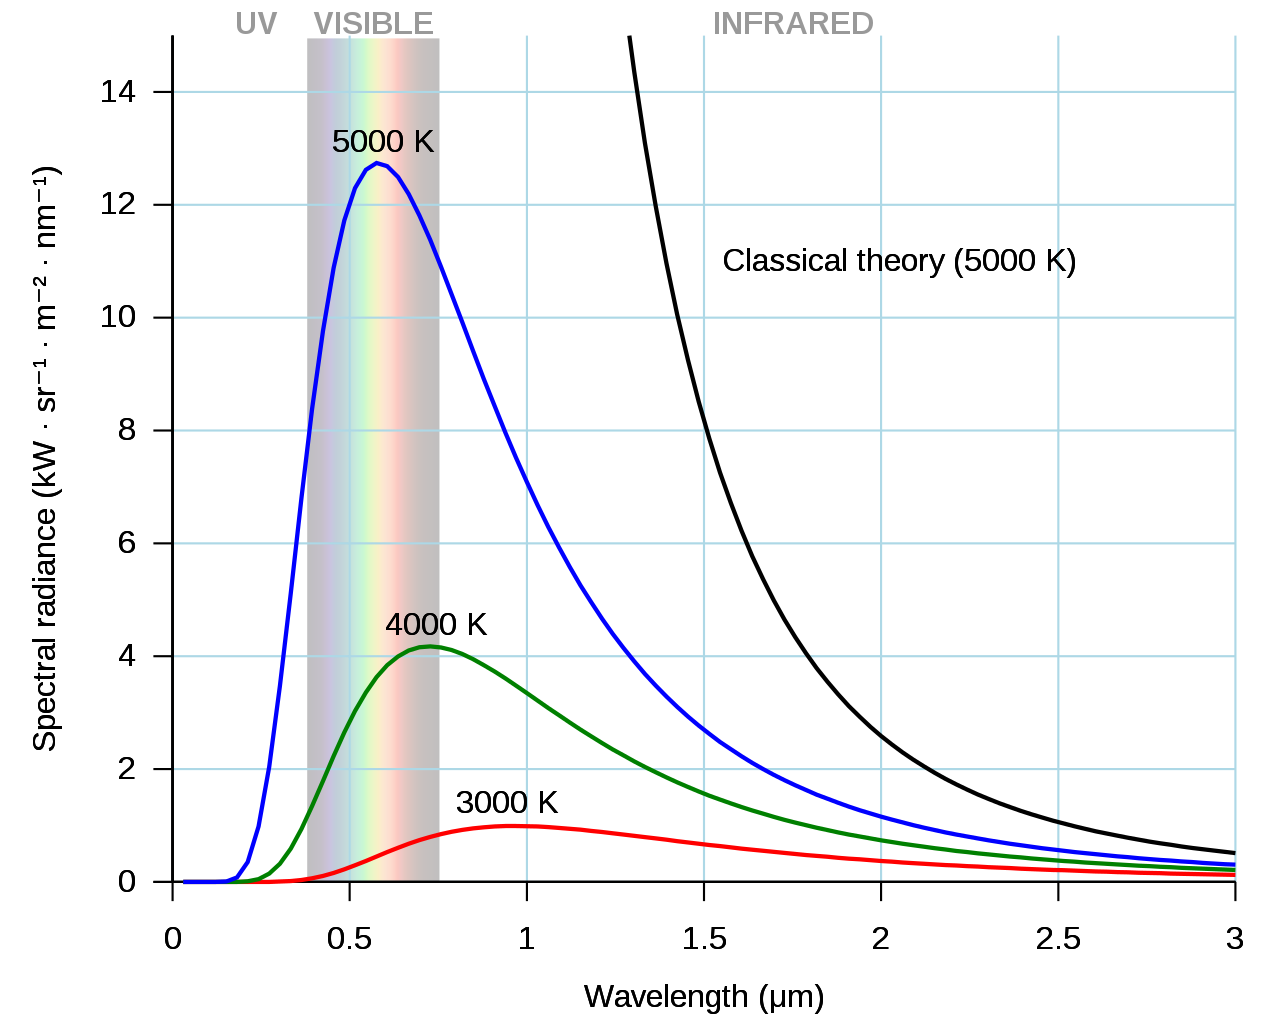
\includegraphics[width=\textwidth]{./images/1280px-Black_body.svg.png}
			\end{figure}
		\end{minipage}
		&
		\begin{minipage}[t]{.45\textwidth}	
			\begin{itemize}\scriptsize
				\item Kirchhoff’s law: 주어진 온도와 파장에서 방출과 흡수의 열역학적 관계\\
				- 복사 에너지를 잘 흡수하는 물체가 복사 에너지를 잘 방출한다.
				\item Planck’s law: 온도에 따른 흑체 복사의 강도 분포를 설명
				- 모든 물체는 항상 다양한 파장의 복사 에너지를 방출한다.
				$$
\begin{gathered}
					I(\nu, T)=\frac{2 h \nu^{3}}{c^{2}} \frac{1}{e^{\frac{h \nu}{k T}}-1} \\
					I^{\prime}(\lambda, T)=\frac{2 h c^{2}}{\lambda^{5}} \frac{1}{e^{\frac{h c}{\lambda k T}}-1}
				\end{gathered}
$$
			\end{itemize}
		\end{minipage}
	\end{tabular}
\end{frame}





\begin{frame}[t]{흑체 복사의 기본 법칙}
	\begin{tabular}{ll}
		\begin{minipage}[t]{.40\textwidth}
			\begin{figure}{}
				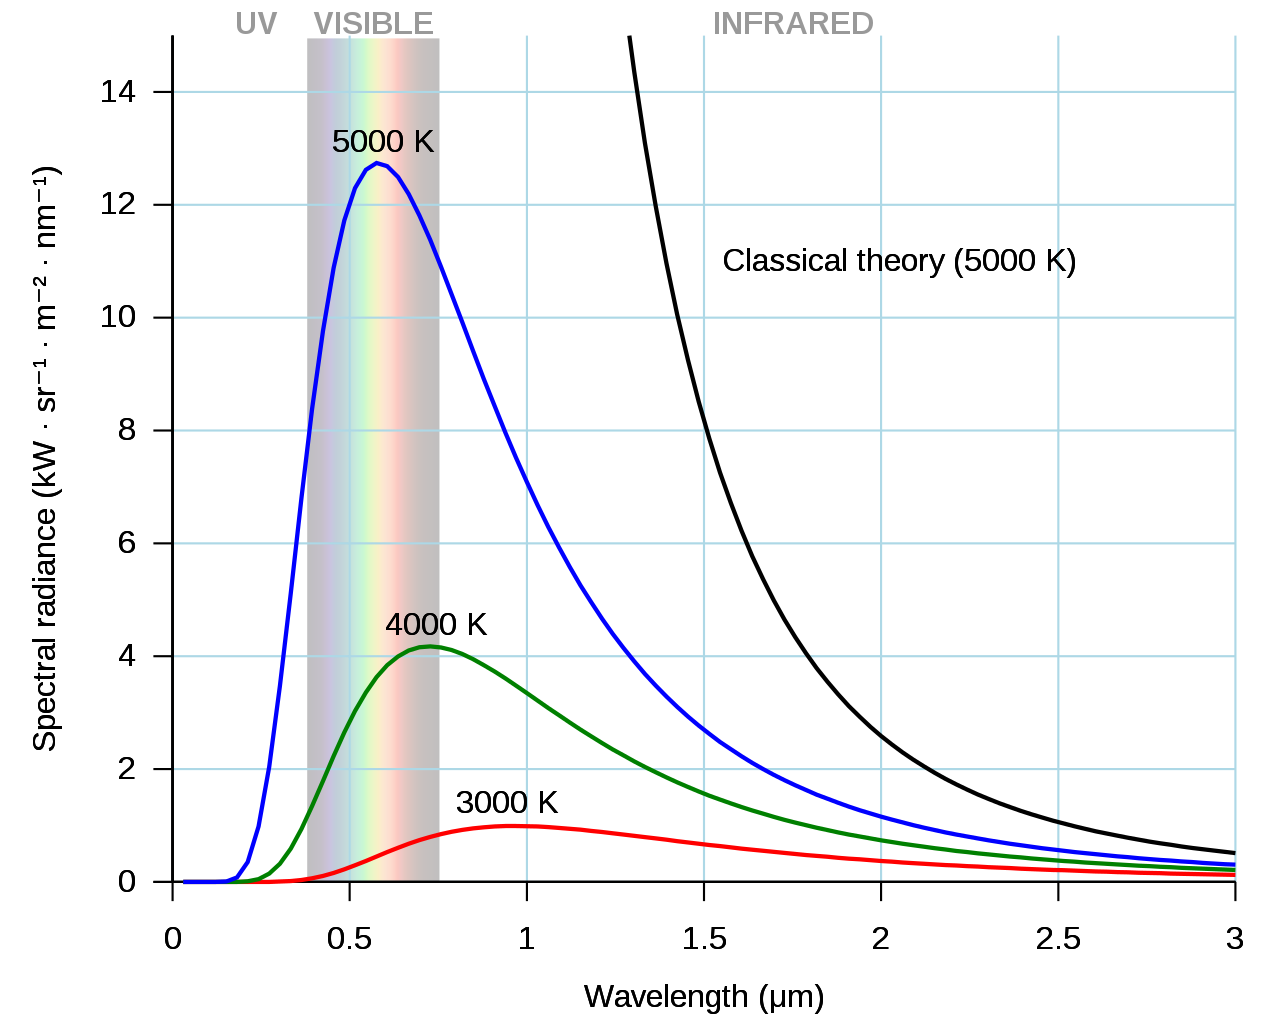
\includegraphics[width=\textwidth]{./images/1280px-Black_body.svg}
			\end{figure}
		\end{minipage}
		&
		\begin{minipage}[t]{.55\textwidth}	
			\begin{itemize}\scriptsize
				\item Stefan-Boltzmann’s law: 방출에너지의 시간변화율과 절대온도와의 관계 \\
				- 물체의 온도가 높을수록 단위 면적당 더 많은 에너지를 방출한다. \\
					$$ \begin{gathered}
						E=\sigma T^{4} \\
						\sigma=\frac{2 \pi^{5} k^{4}}{15 c^{2} h^{3}} = 5.670400 \times 10^{-8} \mathrm{~W} \mathrm{~m}^{-2} \mathrm{~K}^{-4}
					\end{gathered} $$
				\item Wien’s displacement law: 방출하는 최대 강도의 파장과 절대온도와의 관계\\
				- 물체의 온도가 높을수록 최대 복사의 파장은 짧아진다.	\\
					$$
\begin{gathered}
						\lambda_{\max } \cdot T=C \\
						C=2.898 \times 10^{-3} \mathrm{~m} \cdot \mathrm{K}
					\end{gathered}
$$
			\end{itemize}
		\end{minipage}
	\end{tabular}
\end{frame}




\begin{frame}[t]{태양 복사와 지구 복사}
	\begin{tabular}{ll}
		\begin{minipage}[t]{.950\textwidth}
			\begin{figure}{}
				\includegraphics[trim=50 50 30 460, clip, page=72, width=0.9\textwidth]{\bookfile} 
			\end{figure}
			\questionset{태양 복사와 지구 복사에서 자외선, 가시광선, 적외선 복사의 비중은 각각 어느 정도인가?}
			\solutionset{태양 복사:  7\%, 43\%, 49\%   지구 복사: 100\%}			
		\end{minipage}
		&
		\begin{minipage}[t]{.03\textwidth}	
			
		\end{minipage}
	\end{tabular}
\end{frame}



\begin{frame}[t]{자외선과 오존층}
	\begin{tabular}{ll}
		\begin{minipage}[t]{.5\textwidth}
			\begin{figure}{}
				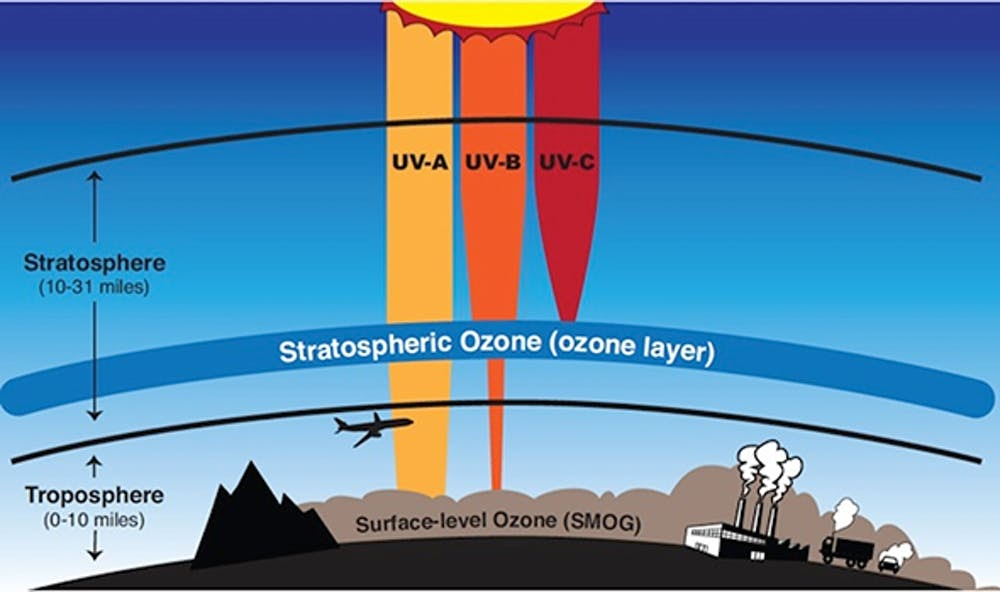
\includegraphics[width=\textwidth]{./images/file-20180418-163998-h02rtb} 
			\end{figure}
		\end{minipage}
		&
		\begin{minipage}[t]{.45\textwidth}
			\begin{figure}{}
				\includegraphics[trim=50 450 330 115, clip, page=74, width=\textwidth]{\bookfile} 
			\end{figure} 
		\end{minipage}
	\end{tabular}
	\begin{itemize}\scriptsize
		\item 자외선은 UVA($320 \sim 400 \rm{~nm}$), UVB($290 \sim 320 \rm{~nm}$), UVC($200 \sim 290 \rm{~nm}$)로 나뉨
		\item UVC는 지구의 표면에 도달하기 전 오존층에서 차단되고, UVA는 1년 내내 노출량이 같고, UVB는 여름에 특히 많아짐.
	\end{itemize}
\end{frame}



\begin{frame}[t]{자외선 지수}
	\begin{tabular}{ll}
		\begin{minipage}[t]{.45\textwidth}
			\begin{figure}{}
				\includegraphics[trim=330 455 55 108, clip, page=73, width=\textwidth]{\bookfile} 
			\end{figure}
			\begin{itemize}\scriptsize
				\item 과도한 자외선은 피부암, 백내장 등을 일으킴
			\end{itemize}
		\end{minipage}
		&
		\begin{minipage}[t]{.5\textwidth}
			\begin{figure}{}
				\includegraphics[trim=355 335 30 205, clip, page=74, width=\textwidth]{\bookfile} 
			\end{figure}	
			
		\end{minipage}
	\end{tabular}
\end{frame}









\section{입사 태양 복사는 어떻게 되는가}


\begin{frame}[t]{태양 복사 에너지의 분포}
	\begin{tabular}{ll}
		\begin{minipage}[t]{.650\textwidth}
			\begin{figure}{}
				\includegraphics[trim=40 40 70 460, clip, page=75, width=\textwidth]{\bookfile} 
			\end{figure}
		\end{minipage}
		&
		\begin{minipage}[t]{.3\textwidth}	
			\questionset{입사한 태양복사가 대기에 도달하면 어떤 일이 발생할 수 있는가?}
			\solutionset{투과 or 흡수 or 반사/산란 하게 하게 된다. \newline}
			
			\questionset{입사한 태양복사의 평균적인 지표, 대기, 구름에서의 분포를 설명하시오}
			\solutionset{지표 흡수: 50\%, \\
				구름, 대기 흡수: 20\%, \\
				구름 반사: 20\%, \\
				대기 후방 산란: 5\%, \\
				지표, 해수면 반사: 5\%}
		\end{minipage}
	\end{tabular}
\end{frame}






\begin{frame}[t]{반사와 산란}
	\begin{tabular}{ll}
		\begin{minipage}[t]{.45\textwidth}
			\begin{figure}{}
				\includegraphics[trim=50 450 335 60, clip, page=76, width=\textwidth]{\bookfile} 
			\end{figure}
		\end{minipage}
		&
		\begin{minipage}[t]{.50\textwidth}	
			\begin{figure}{}
				\includegraphics[width=0.7\textwidth]{./images/XxRaPyyhQGGJWvGpPhUk_Module7-012}
			\end{figure}
			\begin{itemize}\scriptsize
				\item 반사는 빛이 물체의 표면과 만나는 각도와 같은 각도에서 같은 강도로 되돌아 가는 것
				\item 산란은 빛이 약화되어 다른 방향으로 무수히 흩어지는 것
			\end{itemize}	
		\end{minipage}
	\end{tabular}
\end{frame}






\begin{frame}[t]{레일리 산란(Rayleigh scattering)}
	\begin{tabular}{ll}
		\begin{minipage}[t]{.55\textwidth}
			\begin{figure}{}
				\includegraphics[trim=50 535 230 60, clip, page=77, width=\textwidth]{\bookfile} 
			\end{figure}
		\end{minipage}
		&
		\begin{minipage}[t]{.4\textwidth}	
			\begin{itemize}\scriptsize
				\item 산란하는 입자의 크기가 파장보다 훨씬 작은 경우
				\item 산란 강도는 파장의 4제곱에 반비례\\
				$${\displaystyle I \propto	\frac{1}{\lambda^{4}}}$$
				\item 우리 대기의 구성 입자(분자)에 의한 산란이 여기에 해당
			\end{itemize}
		\end{minipage}
			
		\questionset {맑은날 하늘이 파랗게 보이는 이유를 설명하시오.}
		\solutionset{짧은 파장이 더 쉽게 산란되므로 우리 눈에 산란광이 도달하여 하늘이 푸르게 보인다. \newline}

		\questionset{일출이나 일몰 시 하늘이 붉게 보이는 이유를 설명하시오.}
		\solutionset{대기의 광학적 두께가 두꺼워지는 일출, 일몰 시에는 단파장 영역의 빛이 대부분 산란되어 장파장 영역의 빛이 주로 도달하여 하늘이 붉게 보임(노을의 원리)}
	\end{tabular}
\end{frame}





\begin{frame}[t]{미 산란(Mie scattering)}
	\begin{tabular}{ll}
		\begin{minipage}[t]{.600\textwidth}
			\begin{figure}{}
				\includegraphics[width=\textwidth]{./images/scattering} 
			\end{figure}
		\end{minipage}
		&
		\begin{minipage}[t]{.350\textwidth}	
			\begin{itemize}\scriptsize
				\item 먼지와 같은 에어로졸과 빗방울 처럼 산란하는 입자의 크기가 더 커진 경우
				\item 입자 위의 한 점으로부터 산란된 빛과 다른 점으로부터 산란된 빛의 위상이 어긋나 간섭이 발생하며 산란광의 분포도 레일리 산란과 다름
				\item 산란 강도는 파장과 무관함
				\end{itemize}
			
				\questionset {구름이나 안개, 스모그 현상 시 하얗게 보이는 이유는?}
				\solutionset{물방울, 먼지는 빛의 파장보다 크기가 커서 Mie 산란을 일으켜 모든 파장에서 고르게 빛을 산란시키므로}
		\end{minipage}
	\end{tabular}
\end{frame}






\begin{frame}[t]{반사율(albedo)}
	\begin{tabular}{ll}
		\begin{minipage}[t]{.50\textwidth}
			\begin{figure}{}
				\includegraphics[trim=350 50 45 440, clip, page=76, width=\textwidth]{\bookfile} 
			\end{figure}
		\end{minipage}
		&
		\begin{minipage}[t]{.450\textwidth}	
			\begin{itemize}\scriptsize
				\item 지표에 의해 반사된 복사 에너지의 비율
				\item 특정 파장에 대해 정의하지 않고 전 파장영역에 걸친 평균값으로 정의
				\item 입사광의 각도 분포나 대기의 투과율, 지표 성질에 의해서 변화할 수 있는 값
			\end{itemize}
			\questionset {어떤 곳이 알베도가 높은가?}
			\solutionset{눈, 두꺼운 구름, 수면 등 \newline}
			
			\questionset {구름이 알베도에 미치는 영향은 어떨까?}
			\solutionset{낮고 두꺼운 구름은 태양 복사를 반사하여 알베도를 높여 냉각 효과를 일으키고, 높고 얇은 구름은 대부분의 태양 복사가 반사 없이 지표에 도달, 지구 복사는 흡수하여 가열 효과을 일으킨다. 종합적으로는 냉각 효과가 일어난다.}
		\end{minipage}
	\end{tabular}
\end{frame}





\section{대기 중 기체의 역할}


\begin{frame}[t]{태양 복사와 지구 복사}
	\begin{tabular}{ll}
		\begin{minipage}[t]{.55\textwidth}
			\begin{figure}{}
				\includegraphics[trim=270 330 50 230, clip, page=79, width=\textwidth]{\bookfile} 
			\end{figure}
		\end{minipage}
		&
		\begin{minipage}[t]{.40\textwidth}	
			\begin{itemize}
				\item 태양 복사는 자외선, 가시광선, 적외선, 단파복사($2.5 \rm{~\mu m}$ 보다 짧은 파장)
				\item 지구 복사의 대부분은 적외선, 장파복사($2.5 \sim 30 \rm{~\mu m}$)
			\end{itemize}	
			\questionset{태양($5800\rm{~K}$)과 지구($288 \rm{~K}$)의 $\lambda _{\textrm{max}}$ 를 계산해 보자.}
			\solutionset{$$ \begin{gathered}
					\lambda_{\max } \cdot T=C \\
					C=2.898 \times 10^{-3} \mathrm{~m} \cdot \mathrm{K}
				\end{gathered} $$
			태양 : 약 $0.5\rm{~\mu m}$, 지구 : 약 $10\rm{~\mu m}$}
		\end{minipage}
	\end{tabular}
\end{frame}






\begin{frame}[t]{대기를 가열하기}
	\begin{tabular}{ll}
		\begin{minipage}[t]{.350\textwidth}
			\begin{figure}{}
				\includegraphics[trim=270 40 50 230, clip, page=79, width=\textwidth]{\bookfile} 
			\end{figure}
		\end{minipage}
		&
		\begin{minipage}[t]{.60\textwidth}	
			\begin{itemize}
				\item $0.3 \sim 0.7\rm{~\mu m}$ 파장의 가시광에 대해 어떤 기체도 효과적 흡수체가 아니므로 대기는 입사하는 태양 복사에 대해 거의 투명함.
				\item 반면, 장파장인 지구 복사에 대해 상대적으로 효과적인 흡수체이며, 대기는 지구 복사의 약 60\% 정도를 흡수함.(불투명함)
				\item 태양 복사에 대한 효과적인 흡수체는 수증기, 산소, 오존이며, 
				\item 지구 복사에 대한 효과적인 흡수체는 수증기, 이산화 탄소임.
			\end{itemize}	
		\end{minipage}
	\end{tabular}
\end{frame}




\begin{frame}[t]{복사 에너지의 선택적 흡수}
	\begin{tabular}{ll}
		\begin{minipage}[t]{.45\textwidth}
			\begin{figure}{}
				\includegraphics[trim=270 40 50 410, clip, page=79, width=\textwidth]{\bookfile} 
			\end{figure}
		\end{minipage}
		&
		\begin{minipage}[t]{.50\textwidth}	
			\questionset{’대기의 창’이란 무엇이며, 어떤 경우에 닫히기도 하는가?}
			\solutionset{지구 복사 중 $8 \sim 12\rm{~\mu m}$ 파장 대역의 복사는 대기에 의해 거의 흡수되지 않는데, 이를 대기의 창이라고 부른다.\\			
			작은 물방울로 된 구름은 장파 복사를 잘 흡수하며, 이 에너지의 상당 부분을 지표로 방출한다. 따라서 대기의 창을 닫는 역할을 하며, 지표가 냉각되는 속도를 느리게 한다.\newline}
			
			\questionset{기상 위성의 수증기 채널로 사용하기 적합한 파장대는 얼마인가?}
			\solutionset{수증기에 의해서는 흡수되지만 다른 기체에 의해서는 거의 흡수되지 않는 $6 \sim 7 \rm{~\mu m}$ 영역이 수증기를 검출하는데 유용하다.\newline}
			
			\questionset{기상 위성의 적외선 채널은 두 개의 파장대는 얼마이며 이를 구분해주는 기체는 어떤 성분인가?}
			\solutionset{중심파장이 각각 IR1은 $10.8 \rm{~\mu m}$,  IR2는 $12.0 \rm{~\mu m}$ 
			이며, 이 둘의 사이는 산소와 오존에 의해 나누어진다.\newline}
			
		\end{minipage}
	\end{tabular}
\end{frame}








\begin{frame}[t]{복사평형 온도}
	\begin{tabular}{ll}
		\begin{minipage}[t]{.50\textwidth}
			\begin{figure}{}
				\includegraphics[width=0.5\textwidth]{./images/solar_constants} 
			\end{figure}
		\begin{figure}{}
			\includegraphics[trim=0 110 60 85, clip, width=\textwidth]{./images/earth_temp} 
		\end{figure}
		\end{minipage}
			&
		\begin{minipage}[t]{.450\textwidth}
		\questionset{각 행성에서의 태양 상수는 어떻게 되는가? (단, 지구의 태양 상수는 $S_{0}$, 태양- 지구 사이의 평균 거리는 $r_{0}$, 태양 행성 사이의 평균 거리는 $r_{p}$이다.)}
		\solutionset{$$ S_{p}=S_{0}\left(\dfrac{r_{0}}{r_{p}}\right)^{2}$$ \newline}

		\questionset{그림을 참고하여 행성의 복사평형 온도($T_e$)를 식으로 나타내면? (단, 행성의 태양 상수는 $S_{p}$, 행성의 반지름은 $R_{p}$, 반사율 $A$라 하고, 대기의 온실 효과는 고려하지 않는다.)}
		\solutionset{$$
\begin{gathered}
				\pi R_{p}^{2}(1-A) S_{p}=4 \pi R_{p}^{2} \sigma T_{e}^{4} \\
				T_{e}=\left(\frac{1-A}{4 \sigma} S_{p}\right)^{\frac{1}{4}}
			\end{gathered}
$$ }
		\end{minipage}
		\end{tabular}
\end{frame}






\begin{frame}[t]{복사평형 온도}
	\begin{tabular}{ll}
		\begin{minipage}[t]{.20\textwidth}
			\begin{figure}{}
				\includegraphics[width=\textwidth]{./images/temp_of_planets} 
			\end{figure}
		\end{minipage}
		&
		\begin{minipage}[t]{.750\textwidth}			
			\questionset{태양계 행성들의 복사평형 온도를 계산해 보자.}
			\solutionset{실험 시간에 Python으로}
		\end{minipage}
	\end{tabular}
\end{frame}




\begin{frame}[t]{복사평형}
	\begin{tabular}{ll}
		\begin{minipage}[t]{.70\textwidth}
			\begin{figure}{}
				\includegraphics[trim=30 402 30 62, clip, page=81, width=\textwidth]{\bookfile} 
			\end{figure}
			\begin{itemize}\scriptsize
			\item 복사평형(흡수E = 방출E): 행성(위성)들은 태양으로부터 받은 복사에너지와 같은 양의 에너지를 다시 우주 공간으로 방출하여 장기적 관점에서 온도는 일정하게 유지된다.
			\end{itemize}
		\end{minipage}
		&
		\begin{minipage}[t]{.25\textwidth}	
			\questionset{지구와 달의 복사평형 온도는 $255 \rm{~K}$로 같은데, 지구의 평균 온도는 $288 \rm{~K}$인 이유는 무엇인가?}
			\solutionset{지구와 달은 태양과의 평균 거리가 비슷하므로 태양 상수가 같아 복사평형 온도는 $288 \rm{~K}$로 같지만, 지구는 온실효과로 약 $33 \rm{~K}$ 가량 기온이 높게 나타난다.}

		\end{minipage}
	\end{tabular}
\end{frame}





\section{지구의 에너지 수지}




\begin{frame}[t]{에너지 수지}
	\begin{tabular}{ll}
		\begin{minipage}[t]{.80\textwidth}
			\begin{figure}{}
				\includegraphics[trim=55 380 50 60, clip, page=82, width=\textwidth]{\bookfile} 
			\end{figure}
		\end{minipage}
		&
		\begin{minipage}[t]{.150\textwidth}	
			\questionset{지구의 연간 에너지 수지 값을 설명하시오.}
			\solutionset{우주공간, 대기, 지표로 구분하여
				각각 흡수하는 에너지(+)와 방출하는 에너지(-)의 합이 0이 되는지 확인.}
		\end{minipage}
	\end{tabular}
\end{frame}





\begin{frame}[t]{위도별 열수지}
	\begin{tabular}{ll}
		\begin{minipage}[t]{.40\textwidth}
			\begin{figure}{}
				\includegraphics[trim=60 370 360 60, clip, page=83, width=0.8\textwidth]{\bookfile} 
			\end{figure}
		\end{minipage}
		&
		\begin{minipage}[t]{.550\textwidth}	
			\questionset{그림과 같이 적도 지방과 극 지방 사이의 열 불균형이 나타나는 이유와 열 불균형으로 인해 나타나는 현상은?}
			\solutionset{적도 지방은 일반적으로 태양의 고도가 높아 입사하는 복사 에너지가 방출되는 복사보다 많지만, 극 지방은 반대가 되기 때문에 해류와 바람을 통해 적도 지방의 누적된 열이 극지방으로 이동한다.}
		\end{minipage}
	\end{tabular}
\end{frame}

 
	%%%%%%%%%%% *** The Title %%%%%%%%%%
\title[]{기온\\\small{제3장}}

\begin{frame}[plain] %title page
	\titlepage
\end{frame}


\section{기록: 기온 자료}

\begin{frame}[t]{기본 계산}
	\begin{tabular}{ll}
		\begin{minipage}[t]{0.90\textwidth}
			\begin{itemize}
				\item 일평균 기온(daily mean temperature)
				: 24시간 동안 시간별로 얻어진 자료를 평균하거나 24시간 동안
				의 최고, 최저 기온을 평균한 값
				\item 일교차(daily temperature range)
				: 하루 중 최고 기온과 최저 기온의 차이
				\item 월평균 기온(monthly mean temperature)
				: 한 달의 일평균 기온을 모두 더해 그 달의 날 수로 나눈 값(일평균 기온의 평균값)
				\item 연평균 기온(annual mean temperature)
				: 열두 달의 월평균 기온을 모두 더해 12로 나눈 값(월평균 기온의 평균값)
				\item 연교차(annual temperature range)
				: 가장 더운 달과 가장 추운 달의 월평균 기온의 차이
			\end{itemize}			
		\end{minipage}
		&
	\end{tabular}
\end{frame}




\begin{frame}[t]{등온선(isotherms)}
	\begin{tabular}{ll}
		\begin{minipage}[t]{0.60\textwidth}
			\begin{figure}[t]
				\includegraphics[trim=40 425 190 50, clip, page=93, width=\textwidth]
				{\bookfile}
			\end{figure}
		\end{minipage}	
		&
		\begin{minipage}[t]{0.35\textwidth} \scriptsize
			\begin{itemize}
				\item 같은 온도인 지점을 연결한 선으로, $5 \rm{^\circ}C$ 또는 $10\rm{^\circ}C$ 온도 간격으로 많이 표시함. 
				\item 넓은 지역에 걸친 기온의 분포를 눈으로 쉽게 알 수 있도록 보여주기 위해 사용
				\item 단위 거리에 따른 온도 변화 정도를 온도 경도라고 함.
				\item 등온선 간격이 가까우면 급격한 온도 변화를 나타냄.
				
			\end{itemize}
		\end{minipage}
	\end{tabular}
\end{frame}




\begin{frame}[t]{가장 더운 곳}
	\begin{tabular}{ll}
		\begin{minipage}[t]{0.50\textwidth}	
			\begin{figure}[t]
				\includegraphics[trim=365 445 35 90, clip, page=92, width=\textwidth]
				{\bookfile}
			\end{figure}
		\end{minipage}	
		&
		\begin{minipage}[t]{0.45\textwidth}
			\questionset{여름철 캘리포니아의 데스 밸리에서는 왜 최고 기온이 매우 높게 나타나는가?}
			\solutionset{데스 밸리의 고도는 $–53\rm{~m}$이고, 주위 산의 영향으로 인해 바다로부터 유입되는 수증기가 매우 적고 산을 넘어오는 공기 덩어리의 단열 압축으로 인하여 기온이 높고 깨끗한 하늘을 가진다. \\
			이에 따라 이 지역은 태양 복사가 강하고 강수량이 적어 건조하다. 그러므로 수증기의 증발로 소모되는 에너지가 적기 때문에 대부분의 에너지는 지표면을 데우는 데 사용된다. 이로 인해 이 지역의 기온은 매우 높다.}
		\end{minipage}
	\end{tabular}
\end{frame}







\section{온도는 왜 변화하는가: 온도의 제어}


\begin{frame}[t]{온도 제어 요인}
	\begin{tabular}{ll}
		\begin{minipage}[t]{0.95\textwidth}
			\questionset{온도 제어 요인에는 무엇이 있는가?}
			\solutionset{위도, 육지와 물의 차등 가열, 해류, 고도, 지리적 위치, 알베도 변화 등}
		\end{minipage}	
		&
		\begin{minipage}[t]{\textwidth}
		\end{minipage}
	\end{tabular}
\end{frame}





\begin{frame}[t]{위도}
	\begin{tabular}{ll}
		\begin{minipage}[t]{0.40\textwidth}
			\begin{figure}[t]
				\includegraphics[trim=50 330 320 55, clip, page=94, width=\textwidth]
				{\bookfile}
			\end{figure}
		\end{minipage}	
		&
		\begin{minipage}[t]{0.55\textwidth}
			\begin{itemize}
				\item 위도에 따라 태양각과 낮의 길이가 다르다
				\item 그러므로 기본적으로 저위도에서는 온도가 높고, 고위도에서는 온도가 낮다
				\item 주어진 위도에서 계절별 온도 변동은 태양 적위의 변화에 의해 발생한다.				
			\end{itemize}
		\end{minipage}
	\end{tabular}
\end{frame}



\begin{frame}[t]{육지와 물의 차등 가열}
	\begin{tabular}{ll}
		\begin{minipage}[t]{0.35\textwidth}
			\begin{figure}[t]
				\includegraphics[trim=350 35 50 355, clip, page=94, width=\textwidth]
				{\bookfile}
			\end{figure}
		\end{minipage}	
		&
		\begin{minipage}[t]{0.6\textwidth}\scriptsize
			\begin{itemize}
				\item 그림처럼 가열될 때는 육지가 바다보다 빠르게 가열되어 육지의 온도가 해수면의 온도보다 더 높음.
				\item 반대로 냉각될 때는 육지가 바다보다 빠르게 냉각되어 육지의 온도가 해수면의 온도보다 더 낮음.
				\item 기온의 변동은 육지로 덮여 있는 지역이 물로 덮여 있는 지역보다 더 크다.
			\end{itemize}
				\questionset {육지와 물의 가열과 냉각이 다르게 일어나는 이유를 설명하시오.}
				\solutionset{1)물의 큰 유동성 : 물이 가열되면 대류에 의해 깊은 지역까지 열을 분배하지만, 땅은 유체가 아니므로 혼합이 일어나지 않는다. \\
				2) 불투명한 지표면, 투명한 물 : 지표면은 불투명하여 오직 표면에서만 태양 복사가 흡수되지만, 물은 지표면보다는 태양 복사를 더 투과 시키므로 수 미터의 깊이까지 태양 복사가 전달된다.\\ 
				3) 물의 육지의 비열 차이 : 물의 비열이 육지의 비열 보다 3배 이상 크다.\\
				4) 수면에서의 증발 : 물의 기화열, 승화열이 매우 크고, 수면에서의 증발이 지면에서의 증발보다 더 많은 에너지를 필요로 한다.}
		\end{minipage}
	\end{tabular}
\end{frame}



\begin{frame}[t]{육지와 물의 차등 가열}
	\begin{tabular}{ll}
		\begin{minipage}[t]{0.45\textwidth}
			\begin{figure}[t]
				\includegraphics[trim=340 410 40 60, clip, page=95, width=\textwidth]
				{\bookfile}
			\end{figure}
		\end{minipage}	
		&
		\begin{minipage}[t]{0.5\textwidth}
			\questionset{제시된 그래프의 두 지역의 연교차를 비교하고, 그 이유를 설명하시오.}
			\solutionset{같은 위도에 위치하여 유사한 태양각과 낮의 길이를 가지고 있지만 연간 온도변화 폭은 다르다 \\
			육지의 영향을 받는 위니펙의 연간 기온 변화가  바다의 영향을 받는 벤쿠버 보다 크다.}
		\end{minipage}
	\end{tabular}
\end{frame}



\begin{frame}[t]{육지와 물의 차등 가열}
	\begin{tabular}{ll}
		\begin{minipage}[t]{0.6\textwidth}
			\begin{figure}[t]
				\includegraphics[trim=50 450 120 50, clip, page=96, width=0.9\textwidth]
				{\bookfile}
			\end{figure}
		\end{minipage}	
		&
		\begin{minipage}[t]{0.35\textwidth}
			\begin{figure}[t]
			\includegraphics[trim=40 30 350 580, clip, page=96, width=\textwidth]
			{\bookfile}
		\end{figure}
		\end{minipage}
	\end{tabular}
		\newline
		
		\questionset{위의 그림과 표를 참고하여 남반구와 북반구의 연교차를 비교하여 설명하시오.}
		\solutionset{남반구는 81\% 해양, 19\% 육지로 구성, 북반구는 61\% 해양, 39\% 육지로 구성 \\
		⇒ 해양이 지배적인 남반구에서 기온의 연교차가 작다}
\end{frame}





\begin{frame}[t]{해류}
	\begin{tabular}{ll}
		\begin{minipage}[t]{0.90\textwidth}
			\begin{figure}[t]
				\includegraphics[trim=10 430 40 62, clip, page=97, width=0.85\textwidth]
				{\bookfile}
			\end{figure}
		\end{minipage}	
		&
		\begin{minipage}[t]{0.05\textwidth}

		\end{minipage}
	\end{tabular}

		\begin{itemize} \scriptsize 
			\item 난류와 한류는 해안과 인접한 지역의 겨울과 여름철 기온에 큰 영향
			\item 난류의 효과는 겨울에 잘 나타나며, 한류의 효과는 여름에 잘 나타남.				
		\end{itemize}
\end{frame}





\begin{frame}[t]{해류}
	\begin{tabular}{ll}
		\begin{minipage}[t]{0.475\textwidth}
			\begin{figure}[t]
				\includegraphics[trim=140 550 300 60, clip, page=97, width=0.85\textwidth]
				{\bookfile}
			\end{figure}
		
		\begin{itemize} \scriptsize 
			\item 위도가 $52 \rm{{^\circ}N}$인 베를린과 $40 \rm{{^\circ}N}$인 뉴욕의 1월 평균 기온 비슷
		\end{itemize}
		\end{minipage}	
		&
		\begin{minipage}[t]{0.475\textwidth}
			\begin{figure}[t]
				\includegraphics[trim=220 480 230 140, clip, page=97, width=0.85\textwidth]
				{\bookfile}
			\end{figure}
		
		\begin{itemize} \scriptsize 
			\item 남위 23도인 윌비스베이는 남위 29도인 더반보다 여름철에 더 서늘함				
		\end{itemize}
		\end{minipage}
	\end{tabular}
%		\begin{itemize} \scriptsize 
%			\item 북위 52도인 베를린과 북위 40도인 뉴욕의 1월 평균 기온 비슷
%			\item 남위 23도인 윌비스베이는 남위 29도인 더반보다 여름철에 더 서늘함				
%		\end{itemize}
\end{frame}


%			\begin{figure}[t]
%				\includegraphics[trim=350 30 40 480, clip, page=96, width=\textwidth]
%				{\bookfile}
%			\end{figure}




\begin{frame}[t]{해류}
	\begin{tabular}{ll}
		\begin{minipage}[t]{0.50\textwidth}
			\begin{figure}[t]
				\includegraphics[trim=330 30 40 465, clip, page=97, width=\textwidth]
				{\bookfile}
			\end{figure}
		\end{minipage}	
		&
		\begin{minipage}[t]{0.45\textwidth}
			\questionset{제시된 그래프의 두 지역의 여름 기온을 비교하고, 그 이유를 설명하시오.}
			\solutionset{두 지역은 해수면 정도 고도의 연안 도시인데, 적도에 더 가까운 아리카의 여름 기온이 리우데자네이루보다 낮게 나타난다. \\
			아리카는 한류의 영향을 받는 지역이며, 리우데자네이루는 난류의 영향을 받는 지역이기 때문이다.}
		\end{minipage}
	\end{tabular}
\end{frame}




\begin{frame}[t]{고도}
	\begin{tabular}{ll}
		\begin{minipage}[t]{0.450\textwidth}
			\begin{figure}[t]
				\includegraphics[trim=350 30 40 460, clip, page=98, width=\textwidth]
				{\bookfile}
			\end{figure}
		\end{minipage}	
		&
		\begin{minipage}[t]{0.5\textwidth}
			\begin{itemize} \scriptsize 
				\item 위도가 비슷하더라도 고도가 높은 지역의 기온이 낮고 연교차도 작다.
				\item 위도가 비슷하더라도 고도가 높은 지역의 일교차가 더 크다.
			\end{itemize}			
			
			\questionset{고도가 높은 지역의 일교차가 큰 이유를 설명하시오.}
			\solutionset{고도가 증가함에 따라 대기 압력과 밀도도 감소한다. 고도가 올라갈수록 밀도가 감소하므로 특정 고도 위의 대기는 태양복사 중 적은 양만 흡수, 반사, 산란한다. 즉, 고도가 증가하면 주간 태양복사 강도가 증가하여 상대적으로 빠르고 강한 가열이 이루어지고, 반대로 야간에는 냉각이 급속히 이루어진다.}
		\end{minipage}
	\end{tabular}
\end{frame}




\begin{frame}[t]{지리적 분포}
	\begin{tabular}{ll}
		\begin{minipage}[t]{0.50\textwidth}
			\begin{figure}[t]
				\includegraphics[trim=35 50 350 470, clip, page=99, width=\textwidth]
				{\bookfile}
			\end{figure}
		\end{minipage}	
		&
		\begin{minipage}[t]{0.45\textwidth}
			\begin{itemize} \scriptsize 
				\item 해양에서 부는 바람의 영향을 받는 지역(풍상측)이, 육지에서 부는 바람의 영향을 받는 지역(풍하측)에 있는 지역보다 연교차가 작게 나타남
				\item 편서풍 대의 대륙 서안 기후(풍상측), 대륙 동안 기후(풍하측)
			\end{itemize}	
		\end{minipage}
	\end{tabular}	
\end{frame}




\begin{frame}[t]{지리적 분포}
	\begin{tabular}{ll}
		\begin{minipage}[t]{0.50\textwidth}
			\begin{figure}[t]
				\includegraphics[trim=330 450 40 50, clip, page=99, width=\textwidth]
				{\bookfile}
			\end{figure}
		\end{minipage}	
		&
		\begin{minipage}[t]{0.45\textwidth}
		\questionset{시애틀과 스포캔은 불과 $360 \rm{~km}$밖에 떨어져 있지 않지만 연교차는 매우 다르다. 그 이유를 설명하시오.}
		\solutionset{워싱턴 주의 시애틀과 스포캔은 캐스캐이드 산맥이 두 도시를 분리한다. 결론적으로 시애틀은 바다의 영향을 많이 받는데 비해 스포캔은 전형적인 대륙의 영향을 나타낸다.}
		\end{minipage}
	\end{tabular}
			
\end{frame}



\begin{frame}[t]{알베도 변화}
	\begin{tabular}{ll}
		\begin{minipage}[t]{0.450\textwidth}
			\begin{figure}[t]
				\includegraphics[trim=50 420 340 50, clip, page=100, width=\textwidth]
				{\bookfile}
			\end{figure}
		\end{minipage}	
		&
		\begin{minipage}[t]{0.5\textwidth}
			\begin{itemize} \scriptsize 
				\item 운량은 일 최고기온을 낮추고, 최저기온을 높여 일교차를 작게 함.
				\item 운량이 많으면 알베도가 증가하여 태양복사를 
				반사시켜 최고 기온을 낮춤
				\item 운량이 많으면 야간에는 지구 복사를 흡수하고, 
				일부를 지표로 방출함. 
				\item 그러므로 구름 낀 날 야간의 기온이 맑은 날보다 높음.
				
			\end{itemize}			
		\end{minipage}
	\end{tabular}
	
\end{frame}



\begin{frame}[t]{알베도 영향}
	\begin{tabular}{ll}
		\begin{minipage}[t]{0.450\textwidth}
			\begin{figure}[t]
				\includegraphics[trim=350 390 30 50, clip, page=100, width=0.9\textwidth]
				{\bookfile}
			\end{figure}
		\end{minipage}	
		&
		\begin{minipage}[t]{0.5\textwidth}
			\begin{itemize} \scriptsize 
				\item 운량은 월평균 기온에 영향을 미침. 
				\item 예를 들어, 여름에는 우기이므로 구름의 양이 많아져서 태양복사의 지표 입사를 줄이는 반면, 봄에는 건기이므로 하늘이 상대적으로 맑아 태양복사가 지표로 도달하는 양이 많아져서 최고 기온이 4, 5월임.
			\end{itemize}			
		\end{minipage}
	\end{tabular}
	
\end{frame}



\begin{frame}[t]{알베도 영향}
	\begin{tabular}{ll}
		\begin{minipage}[t]{0.50\textwidth}
			\begin{figure}[t]
				\includegraphics[trim=350 0 30 550, clip, page=100, width=\textwidth]
				{\bookfile}
			\end{figure}
		\end{minipage}	
		&
		\begin{minipage}[t]{0.45\textwidth}
			\begin{itemize} \scriptsize 
				\item 지표의 눈과 얼음은 알베도를 높여서 최고 기온은 낮춤.
				\item 해빙의 양의 증가는 알베도를 낮춰서 북극의 온도를 높임.
			\end{itemize}			
		\end{minipage}
	\end{tabular}
	
\end{frame}








\section{전 세계 기온의 분포}


\begin{frame}[t]{1월의 기온 분포}
	\begin{tabular}{ll}
		\begin{minipage}[t]{0.90\textwidth}
			\begin{figure}[t]
				\includegraphics[trim=40 20 60 455, clip, page=101, width=0.8\textwidth]
				{\bookfile}
			\end{figure}
		\end{minipage}	
		&
		\begin{minipage}[t]{0.05\textwidth}
		\end{minipage}
	\end{tabular}	

		\questionset {제시된 그림은 1월의 세계 온도분포를 나타낸 것이다. 등온선이 일반적으로 동-서로 평행한 패턴을 보이는 이유는 무엇인가?}
		\solutionset {위도에 따라 태양의 남중고도와 낮의 길이가 달라져서 태양 복사 에너지가 달라지기 때문에, 적도에서 극으로 갈수록 온도는 감소한다.}		
		
\end{frame}



\begin{frame}[t]{7월의 기온 분포}
	\begin{tabular}{ll}
		\begin{minipage}[t]{0.90\textwidth}
			\begin{figure}[t]
				\includegraphics[trim=40 20 50 455, clip, page=102, width=0.8\textwidth]
				{\bookfile}
			\end{figure}
		\end{minipage}	
		&
		\begin{minipage}[t]{0.05\textwidth}
		
		\end{minipage}
	\end{tabular}
	
		\questionset {제시된 그림은 7월의 세계 온도분포를 나타낸 것이다. 북반구 여름철, 대륙에 
			걸친 등온선은 어느 쪽으로 구부러져 있는지 그 이유와 함께 설명하시오. }
		\solutionset {북반구 여름철에는 물의 비열이 땅의 3배 정도이므로 해양의 온도가 대륙의 온도에 비해 쉽게 오르지 않아서, 대륙에서는 극쪽으로 해양의 경계에서는 적도 쪽으로 구부러져 있다.}	
		
\end{frame}




\begin{frame}[t]{세계의 기온 분포}
	\begin{tabular}{ll}
		\begin{minipage}[t]{0.4750\textwidth}
			\begin{figure}[t]
				\includegraphics[trim=40 20 60 455, clip, page=101, width=\textwidth]
				{\bookfile}
			\end{figure}
		\end{minipage}	
		&
		\begin{minipage}[t]{0.475\textwidth}
			\begin{figure}[t]
			\includegraphics[trim=40 20 50 455, clip, page=102, width=\textwidth]
			{\bookfile}
		\end{figure}	
		\end{minipage}
	\end{tabular}
	
	\questionset {제시된 그림은 1월과 7월의 세계 온도분포를 나타낸 것이다. 등온선이 해류의 존재를 어떻게 보여주는지 설명하시오. }
	\solutionset {난류가 흐르는 곳은 등온선이 극 쪽으로 굽어지며, 한류가 흐르는 곳은 등온선이 적도 쪽으로 굽어지게 한다. 그러므로 난류가 흐르는 지역의 온도는 같은 위도 지역보다 온도가 높고, 한류가 흐르는 지역의 온도는 같은 위도 지역보다 온도가 낮다. \newline}
	
	\questionset{제시된 그림은 1월과 7월의 세계 온도분포를 나타낸 것이다. 등온선이 남반구보다 북반구에서 더 불규칙한 이유를 설명하시오.}
	\solutionset{북반구에는 온도의 변화가 점진적으로 일어나는 해양보다 대륙이 더 많이 분포되어 있기 때문이다.}
	
\end{frame}




\begin{frame}[t]{연교차}
	\begin{tabular}{ll}
		\begin{minipage}[t]{0.90\textwidth}
			\begin{figure}[t]
				\includegraphics[trim=40 405 60 60, clip, page=103, width=0.8\textwidth]
				{\bookfile}
			\end{figure}
		\end{minipage}	
		&
		\begin{minipage}[t]{0.05\textwidth}
		\end{minipage}
	\end{tabular}
	
	\questionset{지구에서 연교차가 가장 큰 곳은 어느 지역인가? 이 지역에서 연교차가 큰 이유는 무엇인가?}
	\solutionset{시베리아 지역이다. 해양으로부터 영향을 적게 받는 대륙의 중심부 지역이고, 겨울철에 온도가 매우 낮기 때문이다.}
	
\end{frame}



\begin{frame}[t]{위도별 연교차}
	\begin{tabular}{ll}
		\begin{minipage}[t]{0.40\textwidth}
			\begin{figure}[t]
				\includegraphics[trim=50 250 360 260, clip, page=104, width=\textwidth]
				{\bookfile}
			\end{figure}
		\end{minipage}	
		&
		\begin{minipage}[t]{0.55\textwidth}
			\begin{figure}[t]
				\includegraphics[trim=320 245 30 305, clip, page=104, width=0.8\textwidth]
				{\bookfile}
			\end{figure}
			
			\questionset{적도 근처에서의 연교차와 고위도 지방에서의 연교차를 비교하면 어떻게 되는가?}
			\solutionset{적도 근처는 계절에 따른 태양 고도 차이에 의한 복사량의 차이가 적기 때문에 고위도 지방에 비해 연교차가 작다.}
			
		\end{minipage}
	\end{tabular}
	
	
\end{frame}




\section{기온 주기}

\begin{frame}[t]{기온 일주기}
	\begin{tabular}{ll}
		\begin{minipage}[t]{0.90\textwidth}
			\begin{figure}[t]
				\includegraphics[trim=50 40 80 570, clip, page=104, width=\textwidth]
				{\bookfile}
			\end{figure}
		\end{minipage}	
		&
		\begin{minipage}[t]{0.05\textwidth}
		\end{minipage}
	\end{tabular}

		\questionset{일교차가 큰 날은 어떤 날인가?}
		\solutionset{맑은 날일수록 일교차가 크다. \newline}
		
		\questionset{자동기상관측시스템 (AWS, Automatic Weather Station) 자료를 이용하여 아래와 같이 기온 변화 그래프를 그려보자.}
		\solutionset{실험 시간에 Python 으로}		

\end{frame}



\begin{frame}[t]{일 최저기온}
	\begin{tabular}{ll}
		\begin{minipage}[t]{0.90\textwidth}
			\begin{figure}[t]
				\includegraphics[trim=30 455 50 50, clip, page=105, width=0.8\textwidth]
				{\bookfile}
			\end{figure}
		\end{minipage}	
		&
		\begin{minipage}[t]{0.05\textwidth}
		\end{minipage}
	\end{tabular}
	
	\questionset{하루 중 기온이 가장 낮은 때는 언제인가? 그리고 그 이유는 무엇인가?}
	\solutionset{하루 중 기온이 가장 낮을 때는 해뜨기 직전이다. 해뜨기 전까지 밤새도록 지표면 근처의 공기가 복사 냉각되기 때문에 새벽에 아래 그림과 같이 서리나 안개가 형성된다.}				
\end{frame}



\begin{frame}[t]{기온 일주기}
	\begin{tabular}{ll}
		\begin{minipage}[t]{0.45\textwidth}
			\begin{figure}[t]
				\includegraphics[trim=40 40 350 410, clip, page=105, width=\textwidth]
				{\bookfile}
			\end{figure}
		\end{minipage}	
		&
		\begin{minipage}[t]{0.5\textwidth}
			\questionset{입사되는 태양 복사의 강도가 정오 시간에 강하지만, 하루 중 가장 따뜻한 시간은 오후 3시 경이다. 그 이유를 설명하시오.}
			\solutionset{태양 복사 에너지는 태양의 고도가 가장 높은 정오에 최대이지만, 지표가 흡수한 에너지를 다시 지구복사의 형태로 대기 중으로 전달하는 데에는 시간이 필요하므로 지구 복사 에너지 최대 지점은 오후 시간이다. \\
			흡수하는 태양복사에너지가 방출하는 지구 복사 에너지를 초과하는 한 지표는 계속 가열되므로, 오후에 하루 중 가장 따뜻한 시점이 존재한다.}				
		\end{minipage}
	\end{tabular}
\end{frame}



\begin{frame}[t]{일교차의 변화}
	\begin{tabular}{ll}
		\begin{minipage}[t]{0.90\textwidth}
			\questionset{일교차의 크기는 지역적 요소와 국지적 일기 조건에 따라 상당히 변할 수 있다. 이러한 변화를 유발하는 요인을 네 가지 기술하시오.}
			\solutionset{1) 지역에 따라 태양의 고도각의 변화가 차이가 난다. 태양의 고도각이 큰 곳은 낮 동안 온도변화가 크다. 반면 극지방과 같이 태양의 고도각이 작은 곳은 낮 동안의 온도 변화가 작아서 일교차가 작다.\\
			2) 해양은 비열이 크고 열수송이 활발히 일어나기 때문에 하루 동안 해양의 온도변화는 $1 \rm{{^\circ}C}$보다 작은 편이다. 따라서 바람이 불어오는 쪽의 해안에 위치한 곳은 온도변화가 완만하다.\\
			3) 구름이 많아 흐린 날의 낮에는 태양 복사 에너지의 흡수가 적어 가열이 적고, 밤에는 지구 복사 에너지를 흡수하기 때문에 냉각도 적다. 따라서 흐린 날의 경우 온도 변화가 크지 않다. \\
			4) 대기의 수증기는 장파 복사를 흡수하는 경향이 있으므로 습한 날은 건조한 날에 비해 상대적으로 온도 변화가 크지 않다.}				
		\end{minipage}	
		&
		\begin{minipage}[t]{0.05\textwidth}
		\end{minipage}
	\end{tabular}

\end{frame}


\begin{frame}[t]{인공위성에서 관측한 지표면 온도}
	\begin{tabular}{ll}
		\begin{minipage}[t]{0.90\textwidth}
			\begin{figure}[t]
				\includegraphics[trim=40 440 340 178, clip, page=106, width=0.7\textwidth]
					{\bookfile}
			\end{figure}	
		\end{minipage}	
		&
		\begin{minipage}[t]{0.05\textwidth}
		\end{minipage}
	\end{tabular}
	
		\questionset{테라와 아쿠아 위성에 탑재되어 있는 MODIS를 이용하여 얻은 2월의 평균 지표면 온도를 나타낸 그림에서 흰색 화살표 지점의 대략적인 온도는 얼마인가? 이러한 차이가 나타나는 이유는 무엇일까?}
		\solutionset{-10 도, +10도 정도이다. 이러한 차이는 여러 요인에 의해 나타나겠지만, 주된 요인은 난류의 영향으로 추측된다.}	
\end{frame}



\begin{frame}[t]{도시 열섬(urban heat island)}
	\begin{tabular}{ll}
		\begin{minipage}[t]{0.450\textwidth}
			\begin{figure}[t]
				\includegraphics[trim=50 415 360 60, clip, page=108, width=0.9\textwidth]
				{\bookfile}
			\end{figure}	
		\end{minipage}	
		&
		\begin{minipage}[t]{0.5\textwidth}
			\questionset{도시 열섬 현상에 기여하는 세 가지 요인을 설명하시오.}
			\solutionset{1) 낮 동안 콘크리트, 아스팔트, 높은 빌딩이 태양 복사 에너지를 흡수하여 저장하고 있다가 야간에도 내어 놓기 때문에\\
				2) 시골에 비해 물의 투수율이 적어서 빗물이 빠르게 흐르게 되어 수분 증발량이 크게 줄어들면서, 수증기의 증발에 사용되던 열이 지표면 온도를 증가시키는데 사용되기 때문에\\
				3) 냉난방, 발전소, 공장, 자동차 등으로부터 에너지가 방출되며, 대기 중 에어로졸이 지표에서 방출된 지구 복사 에너지를 일부 흡수하기 때문에}	
		\end{minipage}
	\end{tabular}
\end{frame}



\begin{frame}[t]{도시 열섬(urban heat island)}
	\begin{tabular}{ll}
		\begin{minipage}[t]{0.450\textwidth}
			\begin{figure}[t]
				\includegraphics[trim=220 350 50 80, clip, page=107, width=\textwidth]
				{\bookfile}
			\end{figure}	
		\end{minipage}	
		&
		\begin{minipage}[t]{0.5\textwidth}
			\questionset{도시 열섬 현상을 해결할 수 있는 방안에는 무엇이 있을까?}
			\solutionset{\begin{figure}[t]
					\includegraphics[width=\textwidth]
					{./images/solution_heat_island}
			\end{figure}}	
		\end{minipage}
	\end{tabular}
\end{frame}







\section{온도 측정}



\begin{frame}[t]{액체 온도계}
	\begin{tabular}{ll}
		\begin{minipage}[t]{0.45\textwidth}
			\begin{figure}[t]
				\includegraphics[trim=40 390 350 60, clip, page=109, width=0.9\textwidth]
				{\bookfile}
			\end{figure}
			
		\end{minipage}	
		&
		\begin{minipage}[t]{0.5\textwidth}

			{\scriptsize 액체 온도계 (수은, 알코올 온도계) : 온도가 상승하면 유체의 분자가 더 활동적이고 팽창한다는 원리를 이용}
			
		\end{minipage}	

	\end{tabular}
\end{frame}




\begin{frame}[t]{최고/최저 온도계}
	\begin{tabular}{ll}
		\begin{minipage}[t]{0.90\textwidth}
			\begin{figure}[t]
				\includegraphics[trim=40 40 270 555, clip, page=109, width=0.7\textwidth]
				{\bookfile}
			\end{figure}
		\end{minipage}	
		&
		\begin{minipage}[t]{0.05\textwidth}
			
		\end{minipage}	
	\end{tabular}
	\begin{itemize} \scriptsize 
		\item 최고 온도계: 수은을 이용하는 경우가 많으며, 온도가 내려가면 협착점(제어관)에서 수은이 되돌아가는 것을 방해하여 최고 온도가 기록되게 한다.
		\item 최저 온도계: 밀도가 낮은 알코올을 이용하고 작은 덤벨 모양의 지표가 있어 온도가 낮아지면 표면장력이 작용하여 최저 온도까지 덤벨 모양의 지표를 끌고 간다. (수평으로 설치)
	\end{itemize}	
\end{frame}





\begin{frame}[t]{자기 온도계}
	\begin{tabular}{ll}
		\begin{minipage}[t]{0.5\textwidth}
			\begin{figure}[t]
				\includegraphics[trim=330 510 50 50, clip, page=109, width=\textwidth]
				{\bookfile}
			\end{figure}	
		\end{minipage}	
		&
		\begin{minipage}[t]{0.45\textwidth}
			{\scriptsize 자기 온도계(thermograph) : 온도에 따른 팽창률이 다른 두 가지 종류의 금속판을 붙여 만든 바이메탈 판의 끝에 잉크가 나오는 부분을 장착하고 이 부분이 시간에 따라 이동하는 드럼위의 종이에 닿아 기온의 변화를 연속적으로 기록}

		\end{minipage}
	\end{tabular}
\end{frame}





\begin{frame}[t]{전기적 온도계}
	\begin{tabular}{ll}
		\begin{minipage}[t]{0.5\textwidth}
			\begin{figure}[t]
				\includegraphics[trim=50 430 350 0, clip, page=110, width=\textwidth]
				{\bookfile}
			\end{figure}
		\end{minipage}	
		&
		\begin{minipage}[t]{0.450\textwidth}
			{\scriptsize 전기적 온도계 : 온도가 높아질수록 전기저항이 커져 전류가 감소하는 성질을 가진 서미스터(온도저항기)를 이용하여 온도 변화를 빠르게 측정.}
		\end{minipage}
	\end{tabular}
\end{frame}



%
%\begin{frame}[t]{온도계}
%	\begin{tabular}{lll}
%		\begin{minipage}[t]{0.30\textwidth}
%			\begin{figure}[t]
%				\includegraphics[trim=40 390 350 50, clip, page=109, width=0.9\textwidth]
%				{\bookfile}
%			\end{figure}
%			{\scriptsize 액체 온도계 (수은, 알코올 온도계) : 온도가 상승하면 유체의 분자가 더 활동적이고 팽창한다는 원리를 이용}
%		\end{minipage}	
%		&
%		\begin{minipage}[t]{0.35\textwidth}
%			\begin{figure}[t]
%				\includegraphics[trim=340 510 50 50, clip, page=109, width=\textwidth]
%				{\bookfile}
%			\end{figure}
%			{\scriptsize 온도 기록기 (thermograph) : 온도에 따른 팽창률이 다른 두 가지 종류의 금속판을 붙여 만든 바이메탈 판의 끝에 잉크가 나오는 부분을 장착하고 이 부분이 시간에 따라 이동하는 드럼위의 종이에 닿아 기온의 변화를 연속적으로 기록}
%		
%		\end{minipage}	
%		&
%		\begin{minipage}[t]{0.30\textwidth}
%			\begin{figure}[t]
%				\includegraphics[trim=50 430 350 50, clip, page=110, width=\textwidth]
%				{\bookfile}
%			\end{figure}
%			{\scriptsize 전기적 온도계 : 온도가 높아질수록 전기저항이 커져 전류가 감소하는 성질을 가진 서미스터(온도저항기)를 이용하여 온도 변화를 빠르게 측정.}
%		\end{minipage}
%	\end{tabular}
%\end{frame}
%
%

\begin{frame}[t]{백엽상}
	\begin{tabular}{ll}
		\begin{minipage}[t]{0.450\textwidth}
			\begin{figure}[t]
				\includegraphics[trim=350 40 0 430, clip, page=110, width=\textwidth]
				{\bookfile}
			\end{figure}
		\end{minipage}	
		&
		\begin{minipage}[t]{0.5\textwidth}
			\questionset{의미 있는 기온 기록을 얻기 위해 온도계의 정확성 외에도 고려해야 할 다른 요인에는 무엇이 있는가?}
			\solutionset{온도계의 설치 장소도 중요하다. 지상으로부터 열, 강수, 직접적인 일사를 피해야 하고, 공기의 자유로운 이동이 가능해야 하며, 
			주변에 높은 건물 등이 없는 풀밭에서 측정해야 한다. \\
			이를 위해 우리는 지상에서 $1.5 \rm{~m}$에 온도계가 위치한 백엽상을 사용한다.}
		\end{minipage}	
	\end{tabular}	
\end{frame}



\begin{frame}[t]{온도 눈금}
	\begin{tabular}{ll}
		\begin{minipage}[t]{0.450\textwidth}
			\begin{figure}[t]
				\includegraphics[trim=350 300 50 60, clip, page=111, width=0.7\textwidth]
				{\bookfile}
			\end{figure}
		\end{minipage}	
		&
		\begin{minipage}[t]{0.5\textwidth}
			\questionset{섭씨온도, 화씨온도, 절대온도의 기준점을 쓰고, 각 온도의 관계를 기술하시오.}
			\solutionset{섭씨온도: $0 \rm{{^\circ}C}$, $100 \rm{{^\circ}C}$\\
				화씨온도: $32 \rm{{^\circ}F}$, $212 \rm{{^\circ}F}$ \\
				절대온도: $273 \rm{K}$, $373 \rm{K}$\\
				
				$$	\begin{aligned}
				\left[{ }^{\circ} \mathrm{C}\right] &=\frac{100}{180} \times\left(\left[{ }^{\circ} \mathrm{F}\right]-32\right) \\
				&=[\mathrm{K}]-273
			\end{aligned} $$}
		\end{minipage}	
	\end{tabular}	
\end{frame}



\section{온도 자료의 응용}



\begin{frame}[t]{난방 도일(heating degree days)}
	\begin{tabular}{ll}
		\begin{minipage}[t]{0.50\textwidth}
			% Please add the following required packages to your document preamble:
			% \usepackage{graphicx}
			{\scriptsize
			\begin{table}[]
					\begin{tabular}{r|r|r}
						\hline
						일자 & 일 평균기온  & 난방 도일 \\						\hline
						1  & $12.3 \rm{{^\circ}C}$ & 6    \\						\hline
						2  & $11.8 \rm{{^\circ}C}$ & 6.5  \\						\hline
						3  & $8.3 \rm{{^\circ}C}$  & 10   \\						\hline
						4  & $10.3 \rm{{^\circ}C}$ & 8    \\						\hline
						5  & $15.3 \rm{{^\circ}C}$ & 3    \\						\hline
						6  & $18.3 \rm{{^\circ}C}$ & 0    \\						\hline
						7  & $19.3 \rm{{^\circ}C}$ & 0   \\					\hline
					\end{tabular}%
			\end{table}
		}
		\end{minipage}	
		&
		\begin{minipage}[t]{0.45\textwidth}
			에너지 수요와 소비 측정 지수\\
			평균 온도가 18.3℃보다 낮은 날: “18.3℃ - 해당 날의 평균기온”(1일 난방 도일)\\
			평균 온도가 18.3℃보다 높은 날: 0
		\end{minipage}
	\end{tabular}
\end{frame}



\begin{frame}[t]{냉방 도일(cooling degree days)}
	\begin{tabular}{ll}
		\begin{minipage}[t]{0.50\textwidth}
			% Please add the following required packages to your document preamble:
			% \usepackage{graphicx}
			% Please add the following required packages to your document preamble:
			% \usepackage{graphicx}
			{\scriptsize
				\begin{table}[]
					\begin{tabular}{c|c|c}
						\hline
						일자 & 일 평균기온  & 냉방 도일 \\						\hline
						1  & $22.3 \rm{{^\circ}C}$ & 4    \\						\hline
						2  & $21.8 \rm{{^\circ}C}$ & 3.5  \\						\hline
						3  & $20.3 \rm{{^\circ}C}$ & 2    \\						\hline
						4  & $19.3 \rm{{^\circ}C}$ & 1    \\						\hline
						5  & $18.3 \rm{{^\circ}C}$ & 0    \\						\hline
						6  & $17.3 \rm{{^\circ}C}$ & 0    \\						\hline
						7  & $16.3 \rm{{^\circ}C}$ & 0   \\						\hline
					\end{tabular}%
			\end{table}
			}
		\end{minipage}	
		&
		\begin{minipage}[t]{0.45\textwidth}
			건물을 냉각시키기 위해 필요한 동력의 양을 나타내는 지수\\
			평균온도가 18.3℃보다 높은 날: “해당 날의 평균온도-18.3℃”(1일 냉방 도일)\\
			평균온도가 18.3℃보다 낮은 날: “0”
			
		\end{minipage}
	\end{tabular}
\end{frame}



\begin{frame}[t]{연간 난방/냉방 도일}
	\begin{tabular}{ll}
		\begin{minipage}[t]{0.450\textwidth}
			\begin{figure}[t]
				\includegraphics[trim=350 30 40 440, clip, page=112, width=\textwidth]
				{\bookfile}
			\end{figure}
		\end{minipage}	
		&
		\begin{minipage}[t]{0.5\textwidth}
			\begin{itemize} \scriptsize 
				\item 앞의 방법으로 구한 값을 1년(7월 1일부터 다음 해 6월 30일 까지)동안 더한 값을 각각 연간 난방 도일, 냉방 도일이라고 함.
				\item 보통 연간 난방 도일, 냉방 도일을 구하여 각 지역을 비교하여 분석함.
				\item 500 난방 도일을 나타내는 달보다 1000 난방 도일을 나타내는 달에는 연료 청구비가 2배가 될 것으로 예상.
				\item 연간 총량을 다른 장소와 비교하여 연료 소비량 차이를 비교하는 데 활용
			\end{itemize}	
		\end{minipage}	
	\end{tabular}	
\end{frame}





\begin{frame}[t]{생육 도일(growing degree days)}
	\begin{tabular}{ll}
		\begin{minipage}[t]{0.550\textwidth} 
			% Please add the following required packages to your document preamble:
			% \usepackage{graphicx}
			{\scriptsize 
			\begin{table}[]
					\begin{tabular}{c|c|c}
						\hline
						작물  & 싹트기          & 수확을 위한 생육 도일($10 \rm{{^\circ}C}$ 기준시) \\\hline
						옥수수 &              & 800$\sim$1400         \\	\hline
						콩   &              & 1100$\sim$1300        \\	\hline
						보리  & 125$\sim$162 & 1290$\sim$1540        \\	\hline
						밀   & 143$\sim$178 & 1550$\sim$1680       \\	\hline
					\end{tabular}%
			\end{table}
		}
		\end{minipage}	
		&
		\begin{minipage}[t]{0.4\textwidth}
			\questionset{생육 도일이란 무엇이며, 이 지수를 사용하는 목적은 무엇인가?}
			\solutionset{일평균 기온과 농작물의 생육 최저 평균 온도를 뺀 값의 합으로 
				해당 농작물을 수확하기 위해 적정한 시기를 결정하기 위해 사용한다.}
		\end{minipage}	
	\end{tabular}	
\end{frame}







\begin{frame}[t]{열파(heat wave)}
	\begin{tabular}{lll}
		\begin{minipage}[t]{0.30\textwidth} \scriptsize 
			\begin{figure}[t]
				\includegraphics[trim=420 420 50 110, clip, page=113, width=\textwidth]
				{\bookfile}
			\end{figure}
		\end{minipage}	
		&
		\begin{minipage}[t]{0.35\textwidth} \scriptsize 
			\begin{figure}[t]
				\includegraphics[trim=53 370 325 110, clip, page=114, width=\textwidth]
				{\bookfile}
			\end{figure}
		\end{minipage}	
		&
		\begin{minipage}[t]{0.30\textwidth} \scriptsize 
			\begin{figure}[t]
				\includegraphics[trim=450 380 35 110, clip, page=114, width=0.8\textwidth]
				{\bookfile}
			\end{figure}
		\end{minipage}	
	
	\end{tabular}	
	\begin{itemize} \scriptsize 
		\item 비정상적으로 덮고 습한 날씨가 일반적으로 며칠에서 몇주까지 지속되는 기간
		\item 도시에서 더 심각하며, 특히 노인들이나 가난한 사람들이 피해를 보며, 사망자가 급증함.
	\end{itemize}	
\end{frame}







\begin{frame}[t]{인간 불편 지수}
	\begin{tabular}{ll}
		\begin{minipage}[t]{0.50\textwidth} \scriptsize 
			\begin{figure}[t]
				\includegraphics[trim=40 440 290 55, clip, page=115, width=\textwidth]
				{\bookfile}
			\end{figure}
		\end{minipage}	
		&
		\begin{minipage}[t]{0.45\textwidth} \scriptsize 
			\questionset{열 스트레스 지수(heat stress index)란 무엇인가?}
			\solutionset{온도와 습도는 여름철 인간의 안락에 가장 큰 영향을 주는 요소로, 이 두 요소를 결합하여 불쾌함과 안락함의 정도를 나타내는 것을 말한다. \\ 
			상대습도가 증가함에 따라 겉보기 온도와 열 스트레스가 증가하는데, 예를 들어 기온이 $90 \rm{{^\circ}F}$이고 상대습도가 65\%일 때, 사람들은 $103 \rm{{^\circ}F}$로 느낀다.  반면, 상대습도가 낮을 때는, 겉보기 온도는 실제 기온보다 낮은 값을 나타낼 수 있다.}
		\end{minipage}	
	
	\end{tabular}	

\end{frame}






\begin{frame}[t]{인간 불편 지수}
	\begin{tabular}{ll}
		\begin{minipage}[t]{0.50\textwidth} \scriptsize 
			\begin{figure}[t]
				\includegraphics[trim=290 40 40 470, clip, page=115, width=\textwidth]
				{\bookfile}
			\end{figure}
		\end{minipage}	
		&
		\begin{minipage}[t]{0.45\textwidth} \scriptsize 
			\questionset{풍속냉각 온도 지수(wind-chill Temperature)란 무엇이며, 사용하는 목적은 무엇인가?}
			\solutionset{겨울철 바람이 불면 몸을 냉기에 노출시키고 신체의 열을 유지시키는 능력 감소시켜 더 춥게 느껴지는데 이를 수치화한 것을 말한다. 인간의 피부에서 바람과 추위를 얼마나 느끼는지 계산하기 위해 설계되었다. }
		\end{minipage}	
		
	\end{tabular}	
	
\end{frame}





%\begin{itemize} \scriptsize 
%	\item 지표의 눈과 얼음은 알베도를 높여서 최고 기온은 낮춤.
%	\item 해빙의 양의 증가는 알베도를 낮춰서 북극의 온도를 높임.
%\end{itemize}	

 
	%%%%%%%%%%% *** The Title %%%%%%%%%%
\title[]{수증기와 대기 안정도 \\ \small{제4장}}

\begin{frame}[plain] %title page
	\titlepage
\end{frame}


\begin{frame}[plain] %cc page
	\ccpage
\end{frame}


\section{지구상의 물}


\begin{frame}[t]{물순환(hydrologic cycle)}
	\begin{tabular}{ll}
		\begin{minipage}[t]{0.550\textwidth}
			\begin{figure}[t]
				\includegraphics[trim=40 10 285 475, clip, page=121, width=\textwidth]
				{\bookfile}
			\end{figure}
		\end{minipage}	
		&
		\begin{minipage}[t]{0.4\textwidth} \scriptsize
			\begin{itemize}
				\item 바다, 대기, 대륙 사이의 연속적인 물 교환
				\item 침투(infiltration) : 육지에 내린 비가 땅 속으로 스며드는 것
				\item 유출(runoff) : 육지에 내린 비가 지표면을 따라 흐르는 것
				\item 증발산(evapotranspiration) : 수면과 토양에서 증발과 식물의 증산을 합친 것
			\end{itemize}

		\end{minipage}
	\end{tabular}
\end{frame}




\begin{frame}[t]{물순환(hydrologic cycle)}
	\begin{tabular}{ll}
		\begin{minipage}[t]{0.40\textwidth}
			\begin{figure}[t]
				\includegraphics[trim=40 10 285 475, clip, page=121, width=\textwidth]
				{\bookfile}
			\end{figure}
		\end{minipage}	
		&
		\begin{minipage}[t]{0.55\textwidth} \scriptsize
			\questionset{주어진 그림을 참고하여 물순환 과정을 설명하시오.}
			\solutionset{바다 및 대륙에서 물의 증발로 대기권으로 수증기 유입되어, 강수가 형성될 때까지 수증기가 이동한다. \\
				바다로 내린 강수는 순환 종료되고, 육지로 내린 강수는 침투, 호수나 하천 유입 및 유출하게 되고, 지하수와 유출 대부분은 증발산 통해 대기권으로 다시 유입된다. \newline}
			
			\questionset{해양에서는 증발에 의해 감소되는 물의 양이 강수량과 같지 않다. 그런데도 해수면이 낮아지지 않는 이유는 무엇인가?}
			\solutionset{해양에서는 증발이 강수보다 많다. 차이가 나는 양은 대기를 통해 대륙으로 이동하여 강수의 형태로 내리게 된다. \\
			육지의 증발은 강수보다 적고 차이가 나는 물은 다시 바다로 흘러 들어가 전체 해수의 양은 보전된다. \newline}
		
			\questionset{물 순환의 의의에 대해 설명하시오.}
			\solutionset{잠열의 흡수와 방출을 통해 에너지를 수송한다.}
		\end{minipage}
	\end{tabular}
\end{frame}



\begin{frame}[t]{물의 특성}
	\begin{tabular}{ll}
		\begin{minipage}[t]{0.50\textwidth}
			\begin{figure}[t]
				\includegraphics[trim=40 400 290 50, clip, page=122, width=\textwidth]
				{\bookfile}
			\end{figure}
		\end{minipage}	
		&
		\begin{minipage}[t]{0.45\textwidth} \scriptsize
			\begin{itemize}
				\item 지구 표면에서 대량으로 발견되는 유일한 액체
				\item 한 상에서 다른 상(고체, 액체, 기체)으로 변환 가능함
				\item 고체 상태인 얼음은 액체 상태인 물보다 밀도가 작음
				\item 비열이 커서 온도 변화를 위해 많은 에너지가 요구됨
				\item 대다수의 특성은 물이 수소결합을 하는 특성의 결과임
			\end{itemize}
			
			\questionset{얼음이 물보다 밀도가 작은 이유를 설명하시오.}
			\solutionset{얼음은 가열되면 수소 결합의 일부가 끊어지며 녹는다. 그 결과 액체 속 물분자들은 좀 더 압축된(빽빽한) 배열을 가진다. 그러므로 액체 상의 물이 얼음보다 밀도가 더 크다.}
			
		\end{minipage}
	\end{tabular}
\end{frame}





\section{물의 상태변화}




\begin{frame}[t]{잠열}
	\begin{tabular}{ll}
		\begin{minipage}[t]{0.65\textwidth}
			\begin{figure}[t]
				\includegraphics[trim=40 400 70 50, clip, page=123, width=\textwidth]
				{\bookfile}
			\end{figure}
		\end{minipage}	
		&
		\begin{minipage}[t]{0.3\textwidth} \scriptsize
			\begin{itemize}
				\item 융해 잠열: $0 \rm{{^\circ}C}$의 얼음(고체)이 물(액체)로 변할 때 약 
				$80 \rm{~cal/g}$의 열을 흡수
				\item 기화 잠열: 물이 수증기로 변할 때는 $540 \rm{~cal/g} ~\left(100 \rm{{^\circ}C}\right) \sim600 \rm{~cal/g}~\left(0 \rm{{^\circ}C}\right)$의 열을 흡수함.
				\item 반대의 과정은 동일한 양의 열을 방출하는 것이 필요!
			\end{itemize}
			
		\end{minipage}
	\end{tabular}
\end{frame}





\begin{frame}[t]{상태 변화}
	\begin{tabular}{ll}
		\begin{minipage}[t]{0.60\textwidth}
			\begin{figure}[t]
				\includegraphics[trim=40 450 80 50, clip, page=124, width=\textwidth]
				{\bookfile}
			\end{figure}
		\end{minipage}	
		&
		\begin{minipage}[t]{0.35\textwidth} \scriptsize
			\begin{itemize}
				\item 증발: 액체 $\rightarrow$ 기체, 응결: 기체 $\rightarrow$ 액체
				\item 수증기가 구름을 형성할 때, 응결 잠열이 방출되며, 그 열이 주위 공기를 가열하여 공기 덩이에 부력을 주어 구름 성장에 도움을 줌
				\item 승화: 고체 $\rightarrow$ 기체, 침적: 기체 $\rightarrow$ 고체
				\item 승화에는 드라이아이스가 사라지는 현상이 대표적인 예이며, 침적은 수증기가 잔디나 창문 등에 얼음으로 침적되는 것(서리)이 예시임.
			\end{itemize}

		\end{minipage}
	\end{tabular}
\end{frame}





\section{습도: 공기 중의 수증기}





\begin{frame}[t]{공기 중의 수증기}
	\begin{tabular}{ll}
		\begin{minipage}[t]{0.50\textwidth}
			\begin{figure}[t]
				\includegraphics[trim=40 510 350 50, clip, page=125, width=\textwidth]
				{\bookfile}
			\end{figure}
		\end{minipage}	
		&
		\begin{minipage}[t]{0.45\textwidth} \scriptsize
			\begin{itemize}
				\item 기상학자들은 대기 중의 수증기량을 표현하기 위해 여러 방법들을 사용
			\end{itemize}
			\questionset{달톤의 법칙을 설명하시오.}
			\solutionset{기체들의 혼합물에 의한 전체 압력은 각 성분에 의한 분압의 합과 동일하다. 
				$${\displaystyle	{ 
				p = p_{1}+p_{2}+\cdots + p_{k}=\sum_{1}^{k} p_{n}
				}	}$$
				 \newline}
			\questionset{공기 중의 수증기량을 나타내는 네 가지는 무엇인가?}
			\solutionset{(상대)습도, 절대 습도, 혼합비, 비습}

		\end{minipage}
	\end{tabular}
\end{frame}




\begin{frame}[t]{수증기압과 포화}
	\begin{tabular}{ll}
		\begin{minipage}[t]{.475\textwidth}
			\begin{figure}{}
				\includegraphics[trim=30 410 290 170, clip, page=126, width=0.95\textwidth]{\bookfile} 
			\end{figure}
			\questionset{수증기압이란 무엇인가?}
			\solutionset{전체 대기 압력에서 수증기가 기여한 압력을 수증기압(vapor pressure)라고 한다.}

			\begin{itemize}\scriptsize
				\item 포화 : 증발 속도 = 응결 속도
				\item 포화 수증기압: 포화되었을 때 수증기에 의해 가해진 압력
			\end{itemize}
		\end{minipage}
		&
		\begin{minipage}[t]{.475\textwidth}	
			\begin{figure}{}
				\includegraphics[trim=30 60 290 395, clip, page=126, width=0.95\textwidth]{\bookfile} 
			\end{figure}
		\end{minipage}
	\end{tabular}
\end{frame}




\begin{frame}[t]{기체 법칙}
	\begin{tabular}{ll}
		\begin{minipage}[t]{0.475\textwidth} \scriptsize 
			대기 상태의 기본 변수는 부피, 압력, 온도이다.

			부피는 주로 비부피(specific volume) 또는 밀도(density)로 나타낸다.

				$$	{\displaystyle	{
						\nu=\frac{\Delta V}{\Delta M}\left[L^3 M^{-1}\right] \\
						\rho=\frac{\Delta M}{\Delta V}\left[M L^{-3}\right]			
				}	}$$
				
			$\nu ~ \rho = 1$의 관계가 있다. 
			
			압력은 단위면적당 힘으로 정의되며, 

				$$	{\displaystyle	{
					p = \frac{\Delta F}{\Delta A}
				}	}$$
		\end{minipage}
		&
		\begin{minipage}[t]{0.475\textwidth} \scriptsize 
		
	
		\end{minipage}
	\end{tabular}
\end{frame}




\begin{frame}[t]{이상기체 상태방정식}
	\begin{tabular}{l|l}
		\begin{minipage}[t]{0.475\textwidth} \scriptsize 
			온도 $T$와 압력 $p$ 에서 이상기체의 단위질량 당 부피인 비부피를 $\nu$라 하자.
				그러면 보일의 법칙과 샤를의 법칙으로부터 보일-샤를의 법칙을 다음과 같이 나타낼 수 있다.
				$$	{\displaystyle	{
						p \nu(T,~p)=p_{0} \nu\left(T,~p_{0}\right),
						\quad 
						\frac{\nu \left(T,~p_{0}\right)}{T}=\frac{\nu \left(T_{0},~p_{0}\right)}{T_{0}}
				}	}$$
				$${\displaystyle	{
						p \nu(T, ~p)=\frac{p_{0} \nu \left(T_{0}, ~p_{0}\right)}{T_{0}} T
				}	}$$
				비기체상수(specific gas constant) $R$을 이용하여 다음과 같이 쓸 수 있다.\\
				$${\displaystyle	{
						p \nu = R T
				}	}$$
				질량이 분자량 $M$과 같은 기체의 시료가 있다면 부피는 $V = M\nu$ 이다.\\
				$${\displaystyle	{
						pV= MR T 
				}	}$$	
		\end{minipage}
		&
		\begin{minipage}[t]{0.475\textwidth} \scriptsize 
			경험 법칙인 아보가드로의 법칙은 동일한 압력과 온도에서 같은 부피 안에 같은 수의 분자수를 지니므로 $\bar R = MR$의 양은 모든 기체에서 상수가 되며 이를 보편기체상수라 한다.
			$$ M R = \frac{pV}{T}, \quad p\nu= \frac{\bar {R}}{M} T $$
			$$ \bar R = MR = 8.3144 \left(\rm J ~mol^{-1} K^{-1}\right) $$
			
			비기체상수(specific gas constant)는 보편기체상수를 기체의 분자량으로 나누어 구할 수있다. \\
			$$R = \frac{\bar{R}}{M}$$
			이상 기체 상태방정식은 아래와 같이 쓸 수도 있다.\\
			$$p  =  \rho R T$$
			
		\end{minipage}
	\end{tabular}
\end{frame}




\begin{frame}[t]{절대습도(absolute humidity)}
	\begin{tabular}{l|l}
		\begin{minipage}[t]{0.475\textwidth} \scriptsize
			절대습도: 혼합공기 $1 \rm{~m^3}$에 들어있는 수증기의 양을 $\rm{g}$으로 나타낸 것 \\
			$$ {\displaystyle	{
				\text { 절대습도 }=\frac{\text { 수증기 질량 }(\mathrm{g})}{\text { 공기 부피 }\left(\mathrm{m}^{3}\right)} 
			}	}$$
				
			이상기체 상태방정식으로 밀도를 구하면 
			$$ {\displaystyle	{
				e = {\rho} R T, \quad \rho = \frac{e}{R T}
			}	} $$
			와 같다. 수증기의 밀도($\rho_w$)는 
			$$ {\displaystyle	{
					\rho_{w}=\frac{e}{R_w T}
				} 	} $$
			$$ {\displaystyle	{
				\begin{aligned}
				R = M {\bar {R}} &= 8.3144 \left(\rm J~mol^{-1}~K^{-1}\right)  \\
				&= 8.3144 \left(\rm Pa~m^3~mol^{-1}~K^{-1}\right)
				\end{aligned}
				}	}	$$
		\end{minipage}	
		&
		\begin{minipage}[t]{0.475\textwidth} \scriptsize
			특별기체상수(specific gas constant)는 보편기체상수(${\bar{R}}$)를 기체의 분자량$\left(M\right)$으로 나누어 구할 수있다. 
			$$ {\displaystyle	{
				R = \frac{\bar{R}}{M}
			}	}	$$
			수증기의 기체상수는
				$$ {\displaystyle	{
				{{R_w}}={\frac {R}{M_w}} = {\frac {8.3144}{18}} = 0.461 \left(\rm J~g^{-1}~K^{-1}\right)
				}	}$$

				$$ {\displaystyle	{
						A. H.= \rho_{w}=\frac{e}{R_w T} = 217 \frac{e}{T} \left(\mathrm{g}~\mathrm{m}^{-3}\right)
				} 		} 	$$
				단, 여기에서 $\mathrm{e}: \mathrm{hPa}$, $\mathrm{T}: \mathrm{K}$ 단위이다. 
		\end{minipage}
	\end{tabular}
\end{frame}




\begin{frame}[t]{공기의 평균 분자량}
	\begin{tabular}{l|l}
		\begin{minipage}[t]{0.475\textwidth} \scriptsize 
			공기의 부피를 $V$, $n$ 번째 기체의 질량을 $m_n$ , 분자량을 $M_n$ 이라고 하자
				$$	{\displaystyle	{
						p_{n}=\frac{\bar{R}}{M_{n}} \frac{m_{n}}{V} T
				} 	}	$$
				달톤의 법칙을 적용하면 \\
				$$	{\displaystyle	{
					\begin{aligned}
						p&=\sum p_{n}=\frac{\bar{R} T}{V} \sum \frac{m_{n}}{M_{n}}\\
						p \nu &=\bar{R} T \frac{\sum \frac{m_{n}}{M_{n}}}{\sum m_{n}}\\
						p \nu&=\frac{\bar{R}}{\bar{M}} T
					\end{aligned}
				}	}	$$

				량은 다음과 같이 정의된다. \\
				$$	{\displaystyle	{
						\frac{1}{\bar{M}} \equiv \frac{\sum \frac{m_{n}}{M_{n}}}{\sum m_{n}}
				}	}	$$
			
		\end{minipage}
		&
		\begin{minipage}[t]{0.475\textwidth} \scriptsize 
			
			혼합 기체인 공기의 평균 분자량은 질량 가중값을 사용하는 조화 평균으로 구할 수 있다.\\

			계산된 건조 공기의 평균 분자량은 $28.966 \times 10^{-3} \rm{~kg~{mol}^{-1}}$ 이다. \\
			건조 공기의 비기체상수는
			$${\displaystyle	{
					R = \frac{\bar{R}}{\bar{M}}=2.8704 \times 10^{2} \rm{~J~{kg}^{-1}~{K}^{-1}}
			}	}$$
			
		\end{minipage}
	\end{tabular}
\end{frame}




\begin{frame}[t]{혼합비와 비습}
	\begin{tabular}{ll}
		\begin{minipage}[t]{0.475\textwidth} \scriptsize
			혼합비(Mixing Ratio): 건조 공기 $1 \rm{~kg}$에 들어 있는 수증기의 양을 $ \rm{~g}$으로 나타낸 것
			\\
			$$ {\displaystyle	{
					\text { 혼합비 }=\frac{\text { 수증기 질량 }(\mathrm{g})}{\text { 건조 공기 질량 }(\mathrm{kg})} 
			} 		} 	$$		

			$$ {\displaystyle	{
				M.R.=\frac{m_{w}}{m_{d}}=\frac{\rho_{w}}{\rho_{d}} = 622 \frac{e}{p-e}(\mathrm{g} / \mathrm{kg})
			} 		} 	$$		
			이상기체 상태방정식을 이용해 구해볼 수 있다.
			$$ {\displaystyle	{
					\begin{aligned}
						p&=\rho R T, \quad \rho=\frac{p}{R T} \\
						e&=\rho_w R_w T, \quad \rho_w=\frac{e}{R_w T} \\
						M.R.&=\frac{\rho_w}{\rho_d} = \frac{\frac{e}{R_w T}}{\frac{\left(p-e\right)}{R_d T}} = \frac{M_w}{M_d}\frac{e}{p-e}
					\end{aligned}
			}	} $$
			

		\end{minipage}	
		&
		\begin{minipage}[t]{0.475\textwidth} \scriptsize
			비습(Specific Humidity): 수증기와 혼합되어 있는  $1 \rm{~kg}$에 들어 있는 수증기의 양을 $ \rm{~g}$으로 나타낸 것 	\\
			$$ {\displaystyle	{
				\begin{aligned}
					&\text { 비습 }=\frac{\text { 수증기 질량 }(\mathrm{g})}{\text { 습윤 공기 질량 }(\mathrm{kg})} \\
					&S.H. = \frac{m_{w}}{m_{d}+m_{w}}=\frac{\rho_{w}}{\rho_{d}+\rho_{w}} = 622 \frac{~e~}{p}(\mathrm{g} / \mathrm{kg}) 
				\end{aligned}
			}		} 		$$	
		\end{minipage}
	\end{tabular}
\end{frame}






\begin{frame}[t]{공기 중의 수증기}
	\begin{tabular}{ll}
		\begin{minipage}[t]{0.45\textwidth}
			\begin{figure}[t]
				\includegraphics[trim=330 50 50 440, clip, page=125, width=\textwidth]
				{\bookfile}
			\end{figure}
		\end{minipage}	
		&
		\begin{minipage}[t]{0.5\textwidth} \scriptsize
			\questionset{절대습도와 혼합비는 어떤 공통점과 차이점을 가지는가? }
			\solutionset{특정 양의 공기에 포함된 수증기의 양으로 표현된다는 점은 같으나, 절대 습도는 수증기의 양이 변하지 않음에도 불구하고 공기덩이의 부피 변화(단열 변화)에 따라 값이 변화하게 되지만, 혼합비는 수증기의 양이 변하지 않으면 변화하지 않는다는 점이 다르다. \newline}
			
			\questionset{상대 습도와 이슬점은 절대 습도, 혼합비와 어떻게 다른가? 상대 습도와 이슬점을 사용하는 이유는 무엇인가?}
			\solutionset{절대습도와 혼합비가 공기 중의 실제 수증기의 양을 나타내는 개념인데, 상대습도는 공기가 포화에 얼마나 근접해있는가를 나타내는 지표이다.\\
			절대습도와 혼합비를 직접 측정하기 어렵기 때문에 기상학에서 공기의 수분함유량을 표현하기 위해 주로 상대습도와 이슬점을 사용한다.}
		\end{minipage}
	\end{tabular}
\end{frame}







\begin{frame}[t]{포화 혼합비 곡선}
	\begin{tabular}{ll}
		\begin{minipage}[t]{.475\textwidth}
			\begin{figure}{}
				\includegraphics[trim=390 440 10 60, clip, page=126, width=0.95\textwidth]{\bookfile} 
			\end{figure}
		\end{minipage}
		&
		\begin{minipage}[t]{.475\textwidth}	
			\questionset{공기를 포화 시키는데 필요한 수증기량과 온도의 일반적인 관계를 기술하라.}
			\solutionset{오른쪽 포화 혼합비 곡선과 아래 포화 혼합비 표를 보면 보통 온도가 10℃ 상승하게 되면 포화수증기량이 약 2배씩 커진다.}
		\end{minipage}
	\end{tabular}
	
\end{frame}


\begin{frame}[t]{포화 혼합비}
	\begin{tabular}{ll}
		\begin{minipage}[t]{.45\textwidth}
			\begin{figure}{}
				\includegraphics[trim=400 40 30 490, clip, page=126, width=0.95\textwidth]{\bookfile} 
			\end{figure}
		\end{minipage}
		&
		\begin{minipage}[t]{.5\textwidth}	
			\questionset{이슬점이 $24\rm{{^\circ}C}$인 공기덩이는 이슬점이 이슬점이 $4\rm{{^\circ}C}$인 공기덩이 보다 얼마나 많은 수증기를 포함하고 있는가?}
			\solutionset{온도가 이슬점이 $10\rm{{^\circ}C}$씩 높아지면 수증기량도 보통 $2$ 배씩 증가하므로 이슬점이 $24\rm{{^\circ}C}$인 공기덩이는 이슬점이 이슬점이 $4\rm{{^\circ}C}$인 공기덩이보다 약 $4$배 많은 수증기를 포함하고 있을 것이다.}
		\end{minipage}
	\end{tabular}
	
\end{frame}







\section{상대습도와 노점온도}


\begin{frame}[t]{상대습도와 이슬점}
	\begin{tabular}{ll}
		\begin{minipage}[t]{0.475\textwidth} \scriptsize
			\begin{itemize}
				\item 		상대습도(Relative Humidity) : 특정 온도에서 포화되기 위해 필요한 수증기량과 실제 수증기량의 비율을 나타낸 것\\
				$$ {\displaystyle	{
						\begin{aligned}
							\text { 상대 습도 } &= \frac{\text {현재 수증기압 }(\mathrm{hPa})}{\text {포화 수증기압 }(\mathrm{hPa})} \times 100\left(\%\right) \\
							\text { 상대 습도 } &= \frac{\text {혼합비}(\mathrm{g/kg})}{\text {포화 혼합비}(\mathrm{g/kg})} \times 100\left(\%\right) 
						\end{aligned}
				} 		}		$$
				\item 		이슬점 : 포화되기 위해 냉각되어야 할 온도를 나타낸 것
			\end{itemize}			
		\end{minipage}	
		&
		\begin{minipage}[t]{0.475\textwidth} \scriptsize
				\questionset{서리점은 무엇인지 설명하시오.}
				\solutionset{온도가 $0\rm{{^\circ}C}$ 이하에서 포화가 일어나는 경우 서리점이라고 한다. 온도가 서리점 이하로 내려갈 경우 수증기는 액체를 거치치 않고 바로 침적되어 서리를 만든다.}		
			
		\end{minipage}
	\end{tabular}
\end{frame}






\begin{frame}[t]{상대습도}
	\begin{tabular}{ll}
		\begin{minipage}[t]{.46\textwidth}
			\begin{figure}{}
				\includegraphics[trim=270 50 30 410, clip, page=128, width=0.95\textwidth]{\bookfile} 
			\end{figure}
		\end{minipage}
		&
		\begin{minipage}[t]{.46\textwidth}	
			\begin{figure}{}
				\includegraphics[trim=50 375 230 50, clip, page=130, width=0.95\textwidth]{\bookfile} 
			\end{figure}
		\end{minipage}
	\end{tabular}
		
		\questionset{상대습도를 변화시키는 요인은 무엇인지 설명하시오}
		\solutionset{1) 수증기의 유입이나 제거, 2) 온도변화}

\end{frame}






\begin{frame}[t]{상대습도}
	\begin{tabular}{ll}
		\begin{minipage}[t]{.36\textwidth}
			\begin{figure}{}
				\includegraphics[trim=50 400 380 50, clip, page=131, width=0.95\textwidth]{\bookfile} 
			\end{figure}
		\end{minipage}
		&
		\begin{minipage}[t]{.59\textwidth}	
			\questionset{하루 중 상대습도가 가장 높았을 때와 가장 낮을 때는 언제인가}
			\solutionset{수증기량의 변화가 없다면 상대습도는 온도가 낮아 포화수증기량이 가장 낮은 새벽에 가장 높고, 온도가 가장 높은 오후에 가장 낮다. \newline}
			
			\questionset{하루 중 이슬이 생기기 쉬운 시간은?}
			\solutionset{이슬은 상대습도가 가장 높은 새벽에 나타나기 쉽다. \newline}
			
			\questionset{기온의 변화와 상대습도의 변화와의 일반적인 관계를 기술하라.}
			\solutionset{기온의 변화와 상대습도의 변화는 반비례한다. 즉 기온이 상승하면 상대습도는 하강하고, 기온이 하강하면 상대습도는 상승한다. \newline}
			
			\questionset{온도가 일정하고 혼합비가 감소한다면 상대습도는 어떻게 변하는가?}
			\solutionset{혼합비는 건조공기 $1 \rm{~kg}$에 들어있는 수증기의 양을 g으로 나타낸 것이고, 상대습도는 수증기량을 포화수증기량으로 나눈 것이다. \\
			그런데 혼합비가 감소하므로 수증기량은 감소하고, 온도는 일정하므로 포화 수증기량은 일정하기 때문에 상대습도는 감소한다.	}
		\end{minipage}
	\end{tabular}
\end{frame}





\begin{frame}[t]{상대습도와 수증기}
	\begin{tabular}{ll}
		\begin{minipage}[t]{.4\textwidth}
			\begin{figure}{}
				\includegraphics[trim=230 220 55 90, clip, page=129, width=0.95\textwidth]{\bookfile} 
			\end{figure}
		\end{minipage}
		&
		\begin{minipage}[t]{.55\textwidth}	
			\questionset{데스 밸리는 기온이 $25 \rm{{^\circ}C}$, 상대 습도는 20\% 이고, 시카고는 기온이 $-10 \rm{{^\circ}C}$, 상대 습도는 100\% 일 때, 두 지역에 포함된 수증기의 양을 비교하시오.}
			\solutionset{$-10 \rm{{^\circ}C}$의 포화 혼합비는 $2 \rm{~g/kg}$, $25 \rm{{^\circ}C}$의 포화 혼합비는 $20 \rm{~g/kg}$ 이므로 상대습도가 20\% 인 이 날 데쓰 밸리의 혼합비는 $4 \rm{~g/kg}$로 시카고보다 약 $2$배의 수증기를 포함한다.}
		\end{minipage}
	\end{tabular}
\end{frame}








\begin{frame}[t]{상대습도와 수증기}
	\begin{tabular}{ll}
		\begin{minipage}[t]{.4\textwidth}
			\begin{figure}{}
				\includegraphics[trim=50 50 250 420, clip, page=132, width=0.95\textwidth]{\bookfile} 
			\end{figure}
		\end{minipage}
		&
		\begin{minipage}[t]{.55\textwidth}	
			\questionset{건습계의 원리를 설명하라.}
			\solutionset{건습계는 일반적인 온도계인 건구 온도계와 구부가 물에 젖은 헝겊에 감싸여 있어 온도계를 돌리면서 증발이 일어나면서 에너지를 흡수하여 온도가 낮아지는 습구 온도계로 구성되어 있다. \\
			상대습도가 낮을수록 건구와 습구 온도의 차이가 커지게 되어 상대습도를 알 수 있다. \newline}
		
			\questionset{모발 습도계의 원리는 무엇이며, 단점과 장점은 무엇인가?}
			\solutionset{모발 습도계는 습도가 증가함에 따라 모발이 늘어나는 정도도 비례하여 증가한다는 원리를 이용한 습도계이다. \\
			단점은 건습계에 비해 정확하지 않고, 보정이 자주 필요하고, 특히 온도가 낮은 경우 습도 변화에 반응이 느리다는 점이고, 장점은 건습계는 건구 온도와 습구 온도를 모두 읽은 뒤 표에서 상대습도를 찾아야 하는 반면, 모발 습도계는 상대습도를 눈금으로 바로 읽으면 된다.}		
		\end{minipage}
	\end{tabular}
\end{frame}





\section{단열변화와 구름 형성}


\begin{frame}[t]{단열 변화}
	\begin{tabular}{ll}
		\begin{minipage}[t]{.4\textwidth}
			\begin{figure}{}
				\includegraphics[trim=35 440 290 50, clip, page=135, width=0.95\textwidth]{\bookfile} 
			\end{figure}
		\end{minipage}
		&
		\begin{minipage}[t]{.55\textwidth}	
			\questionset{공기가 대기를 통과하여 위쪽으로 상승하는 동안 공기는 왜 팽창하는지 설명하시오.}
			\solutionset{풍선과 같은 얇은 막을 가진 공기 덩이를 가정하자. 공기가 위로 상승하게 되면 기압이 감소하게 된다. 열의 출입이 없는 상태에서 공기덩이가 위로 상승하게 되면 공기덩이의 압력이 주위 공기의 압력보다 높게 되고, 부피가 증가하면서 일을 해주게 되면서 내부 에너지는 감소하고 기온도 감소하게 된다. \newline}
			
			\questionset{공기가 하강할 때는 왜 가열이 되는지 설명하시오.}
			\solutionset{공기가 하강하면 주변 공기의 압력이 공기덩이의 압력보다 크게 되어 공기덩이는 일을 받게 되고, 단열 상태에서 일을 받게 되면 내부에너지는 증가하여 기온은 상승하게 된다. \newline}
			
			\questionset{휴대용 부탄가스를 사용할때 용기가 차갑게 느껴지는 이유는?}
			\solutionset{내용물이 바깥으로 나오면서 압력이 낮아지고 일을 해주게 되어 내부에너지가 감소하게 되므로 기온이 내려가기 때문이다. \newline}					
		\end{minipage}
	\end{tabular}
\end{frame}



\begin{frame}[t]{단열 변화}
	\begin{tabular}{ll}
		\begin{minipage}[t]{.4\textwidth}
			\begin{figure}{}
				\includegraphics[trim=35 440 290 50, clip, page=135, width=0.95\textwidth]{\bookfile} 
			\end{figure}
		\end{minipage}
		&
		\begin{minipage}[t]{.55\textwidth}	
			\begin{itemize} \scriptsize 
				\item 	단열 변화 : 열의 출입이 없는 상태에서 일어나는 온도변화
				\item 	건조단열감률 : 연직으로 이동하는 불포화된 공기덩어리에 적용하는 온도감률 $10 \rm{{^\circ}C/km}$
				\item 	습윤단열감률 : 연직으로 이동하는 포화된 공기덩어리에 적용하는 온도감률 보통 수분함유량에 따라 약 $5\sim9 \rm{{^\circ}C/km}$
				\item 	이슬점감률 : 공기덩어리가 연직으로 이동하여 단열팽창하면 수증기의 밀도가 감소하여 수증기압도 낮아져서 이슬점이 내려감. 불포화 공기에서는 $2 \rm{{^\circ}C/km}$이며, 포화 공기에서는 해당 습윤단열감률과 동일함. 
			\end{itemize}	

		\end{minipage}
	\end{tabular}
\end{frame}



\begin{frame}[t]{상승 응결 고도}
	\begin{tabular}{ll}
		\begin{minipage}[t]{.4\textwidth}
			\begin{figure}{}
				\includegraphics[trim=335 40 30 350, clip, page=135, width=0.95\textwidth]{\bookfile} 
			\end{figure}
		\end{minipage}
		&
		\begin{minipage}[t]{.55\textwidth}
			\begin{itemize} \scriptsize 
				\item 불포화 상태인 공기가 상승 하여 포화에 도달해 구름이 형성되기 시작하는 고도
				\item 상승응결 고도를 $H$, 지상기온을 $t$, 지상 이슬점을 $t_d$라고 하면 건조 단열 감률은 $1 \rm{{^\circ}C/100~m}$, 이슬점 감률은 $0.2 \rm{{^\circ}C/100~m}$이므로, 
				$${\displaystyle {
					\begin{aligned}
					t-\left(H \times \frac{1^{\circ} \mathrm{C}}{100 \mathrm{m}}\right)&=t_{d}-\left(H \times \frac{0.2^{\circ} \mathrm{C}}{100 \mathrm{m}}\right) \\
					H[{m}]&=125\left({t}-{t}_{d}\right)
					\end{aligned}
				}	}$$
			\end{itemize}			
		\end{minipage}
	\end{tabular}
\end{frame}





\begin{frame}[t]{정적 비열과 정압 비열}
	\begin{tabular}{l|l}
		\begin{minipage}[t]{0.475\textwidth} \scriptsize
			비열은 어떤 물질 $1 \rm{g}$의 온도를 $1 \rm{{^\circ}C}$ 올리는데 필요한 열량이다. \\
			정적비열 ($C_v$): 부피를 일정하게 유지하면서 가열했을 때 물질이 나타내는 비열 \\
			정압비열 ($C_p$): 압력을 일정하게 유지하면서 가열했을 때 물질이 나타내는 비열 \\
			내부에너지 $U$는 사실상 온도와 부피의 함수이며 압력과는 무관하다. \\
			따라서 $U \left(T, V\right)$로 나타낸다. \\
			엔탈피는 온도와 압력에 관한 함수로 $H \left(T, P\right)$로 나타낼 수 있는데, 정의는 $H =  U + PV$ 이다.\\
			정적 비열과 정압 비열을 각각 내부에너지와 엔탈피를 이용하여 표현하면 다음과 같다. \\
			$${\displaystyle	{
					C_{v}=\left(\frac{\partial U}{\partial T}\right)_{v}
					\quad	C_{p}=\left(\frac{\partial H}{\partial T}\right)_{p}
			}	}$$
		\end{minipage}	
		&
		\begin{minipage}[t]{0.475\textwidth} \scriptsize
			$${\displaystyle		{
					\begin{aligned} 
						C_{p} &=\left(\frac{\partial H}{\partial T}\right)_{p} =\left(\frac{\partial(U+P V)}{\partial T}\right)_{p} \\ &=\left(\frac{\partial U}{\partial T}\right)_{p}+P\left(\frac{\partial V}{\partial T}\right)_{p} \\ 
						&=C_{v}+P\left(\frac{\partial\left(\frac{R T}{P}\right)}{\partial T}\right)_{p} =C_{v}+P\left(\frac{R}{P}\right) \\ 
						&=C_{v}+R 
					\end{aligned}
			}	}$$
			
			따라서 정압 비열과 정적 비열사이의 관계는 $C_{p} = C_{v} + R$로 정리할 수 있다.
		\end{minipage}
	\end{tabular}
\end{frame}




\begin{frame}[t]{열역학 제1법칙}
	\begin{tabular}{l|l}
		\begin{minipage}[t]{.475\textwidth} \scriptsize 
			열역학 제 1법칙을 이용하여 ${\Delta q=c_{v} \Delta T+p \Delta \nu}$을 설명하면\\
			어떤 공기덩이에 열량 $\Delta Q$를 가하면 이중 일부는 $\Delta W$ 만큼의 일을 하는데 사용되고, 나머지는 $\Delta U$ 만큼의 내부에너지를 변화시키는데 사용된다.\\
				$$\Delta Q=\Delta U+\Delta W$$
				각 항을 공기덩이의 질량으로 나누어 단위 질량에 대해 다음과 같이 소문자로 나타내면 \\
				$$\Delta q=\Delta u+\Delta w$$
				이상기체라고 가정하면 \\
				$$\Delta u=c_{v} \Delta T$$
				여기에서 $c_{v}$는 정적비열이고, $\Delta T$는 온도 변화량이다.
		\end{minipage}
		&
		\begin{minipage}[t]{.475\textwidth}	\scriptsize 
			일의 물리학적 정의는 
			$${\Delta W=F \Delta S}$$
			반지름 $R$ 인 공 모양의 공기덩이의 압력을 $p$, 그 표면적을 $A$라 하면 
			$${\Delta W = p A \Delta R = p \Delta V}$$
			단위 질량의 공기덩이인 비부피에 대해 다음과 같이 쓸 수 있다. 
			$${\Delta w = p \Delta \nu}$$
			이를 대입하면 ${\Delta q=c_{v} \Delta T+p \Delta \nu}$ 이다.
			
		\end{minipage}
	\end{tabular}
\end{frame}





\begin{frame}[t]{열역학 제1법칙}
	\begin{tabular}{l|l}
		\begin{minipage}[t]{0.475\textwidth} \scriptsize
			${\Delta q=c_{v} \Delta T+p \Delta \nu}$을 ${\Delta q = c_{p} \Delta T - \nu  \Delta p}$로 표현하자면 \\
			공기덩이의 압력이 $p \rightarrow p+\Delta p$, 비부피가 $\nu \rightarrow \nu +\Delta \nu $, 온도가 $T \rightarrow T +\Delta T$로 변화했다면 나중 상태의 상태방정식은 \\
				$${\displaystyle {
						(p+\Delta p)(\nu+\Delta \nu)=R (T+\Delta T)
				} }$$
				$${\displaystyle {
						\\
						p \nu\left(1+\frac{\Delta p}{p}+\frac{\Delta \nu}{\nu}+\frac{\Delta p \Delta \nu}{p \nu}\right)=R T\left(1+\frac{\Delta T}{T}\right)
				} }$$
				
				$p \nu =R T$를 사용하고, $\frac{\Delta p}{p}$, $\frac{\Delta \nu}{\nu}$가 $1$보다 훨씬 작은 양으로 취급하여 $\frac{\Delta p \Delta \nu}{p \nu}$	항을 무시하면\\
				$${\displaystyle {
						\frac{\Delta T}{T}=\frac{\Delta p}{p}+\frac{\Delta \nu}{\nu}
				}		}$$	
		\end{minipage}	
		&
		\begin{minipage}[t]{0.475\textwidth} \scriptsize
			우변에 $RT$를 곱하고, 좌변에 ${p \nu}$를 곱하면\\
			$${\displaystyle {
				\begin{aligned}
					R \Delta T&= \nu \Delta p+p \Delta \nu \\
					p \Delta \nu &= R \Delta T - \nu \Delta p \\
					\Delta q&=c_{v} \Delta T+p \Delta \nu \\
					&= (c_{v}+R) \Delta T - \nu \Delta p
				\end{aligned}
			} 	}$$
		$c_p = c_v+R$ 이므로	\\
		$${\Delta q = c_{p} \Delta T - \nu  \Delta p}$$
		\end{minipage}
	\end{tabular}
\end{frame}





\begin{frame}[t]{건조단열감률}
	\begin{tabular}{l|l}
		\begin{minipage}[t]{0.475\textwidth} \scriptsize
			열역학 제1법칙 $\Delta q = c_{p} \Delta T - \nu  \Delta p$을 미분형으로 쓰면 
				$$	{\displaystyle	{
					d q = c_{p} d T - \nu  d p
				}	}	$$
			단열 변화에서는 $d q = 0$이고, 대기의 정역학적 평형 $dp = - \rho g dz$을 고려하면
				$${\displaystyle	{
					\begin{aligned}
						0 &= c_{p} d T - \nu  d p \\
						0 &= c_{p} d T + g  d z
					\end{aligned}
				}	}	$$		
			식을 정리하면
				$${\displaystyle	{
					- \frac {dT}{dz} = \frac{g}{c_p} = {\Gamma}_{d}
				}	}$$	
		\end{minipage}	
		&
		\begin{minipage}[t]{0.475\textwidth} \scriptsize
			
			
		\end{minipage}
	\end{tabular}
\end{frame}



\begin{frame}[t]{습윤단열감률}
	\begin{tabular}{l|l}
		\begin{minipage}[t]{0.475\textwidth} \scriptsize
			포화 공기는 수증기 응결로 인해 잠열이 방출되므로  $d q \neq 0$ 이다.\\
			포화혼합비를 $W_s$라고 하고, 응결 숨은열을 $L$이라고 하면 
			응결에 의해 단위 질량의 건조 공기가 흡수하는 열량은 $-Ldw_s$이다.
				$${\displaystyle	{
					-Ldw_s = c_{p} d T + gdz
				}	}$$
			양변을 $c_{p} d z$로 나누고 항을 정리하면
			$$	{\displaystyle	{
				\begin{aligned}
					\frac{d T}{d z}&=-\frac{L}{c_{p}} \frac{d w_{s}}{d z}-\frac{g}{c_{p}}\\
					\frac{d T}{d z}&=-\frac{L}{c_{p}} \frac{d w_{s}}{d T} \frac{d T}{d z}-\frac{g}{c_{p}}\\
					\frac{d T}{d z} + \frac{L}{c_{p}} \frac{d w_{s}}{d T} \frac{d T}{d z} &=-\frac{g}{c_{p}}\\
				\end{aligned}
				}	}$$
		\end{minipage}	
		&
		\begin{minipage}[t]{0.475\textwidth} \scriptsize
			$$	{\displaystyle	{
				\begin{aligned}
					\frac{d T}{d z} \left( 1 + \frac{L}{c_{p}} \frac{d w_{s}}{d T} \right)
					=- {\Gamma}_{d}\\
					- \frac{d T}{d z} 
					= \frac{{\Gamma}_{d}}{ 1 + \dfrac{L}{c_{p}} \dfrac{d w_{s}}{d T} } = {\Gamma}_{s}\\
				\end{aligned}
			}	}$$
			$\dfrac{d w_{s}}{d T}$가 항상 양의 값을 가지므로 ${\Gamma}_s < {\Gamma}_d$ 임을 알 수 있다.\\
			$\dfrac{d w_{s}}{d T}$의 값이 큰 온난 다습한 공기는 습윤단열감률이 작고, 대류권계면 부근에서는 습윤단열감률이 건조단열감률과 비슷하다.

			
		\end{minipage}
	\end{tabular}
\end{frame}








\section{공기 덩이를 상승시키는 과정}


\begin{frame}[t]{지형성 상승}
	\begin{tabular}{ll}
		\begin{minipage}[t]{.5\textwidth}
			\begin{figure}{}
				\includegraphics[trim=50 40 220 450, clip, page=136, width=0.95\textwidth]{\bookfile} 
			\end{figure}
		\end{minipage}
		&
		\begin{minipage}[t]{.45\textwidth}
			\begin{itemize} \scriptsize 
				\item 공기덩이가 산악 장애물에 의해 강제 상승
				\item 푄 현상(높새 바람)
				\item 풍상측 경사면은 강수 유발
				\item 풍하측은 비그늘 사막(rain shadow desert)
			\end{itemize}	
			\questionset{겨울철에 강릉 지역이 왜 건조한지 설명하라.}
			\solutionset{겨울철 우리나라는 북서 계절풍이 주로 부는데 북서 계절풍이 산맥을 넘어오면서 수증기가 응결하여 많은 양의 수증기를 잃게 되어 혼합비가 낮아지고, 산맥을 넘어 풍하측인 강릉에 도착할때 단열압축을 하면서 더욱 따뜻한 공기덩이로 변하면서 상대습도가 낮아지게 된다.}
		\end{minipage}
	\end{tabular}
\end{frame}


\begin{frame}[t]{전선 치올림}
	\begin{tabular}{ll}
		\begin{minipage}[t]{.5\textwidth}
			\begin{figure}{}
				\includegraphics[trim=50 40 280 560, clip, page=137, width=0.95\textwidth]{\bookfile} 
			\end{figure}
		\end{minipage}
		&
		\begin{minipage}[t]{.45\textwidth}
			\begin{itemize} \scriptsize 
				\item 			따뜻하고 밀도가 작은 공기덩이가 차고 밀도가 큰 공기덩이 위로 강제 상승
			\end{itemize}	
			\questionset{전선 치올림이 공기를 상승시키는 과정을 설명하시오.}
			\solutionset{따뜻한 공기와 차가운 공기가 만나면 전선면을 만드는데, 밀도가 상대적으로 낮은 따뜻한 공기가 차가운 공기 위로 강제로 올라가면서 단열변화가 나타나게 된다.}

		\end{minipage}
	\end{tabular}
\end{frame}




\begin{frame}[t]{수렴}
	\begin{tabular}{ll}
		\begin{minipage}[t]{.45\textwidth}
			\begin{figure}{}
				\includegraphics[trim=50 440 300 50, clip, page=138, width=0.85\textwidth]{\bookfile} 
			\end{figure}
			\begin{itemize} \scriptsize 
				\item 			수평적 공기 흐름에 의해 쌓인 공기가 상승
			\end{itemize}
		\end{minipage}
		&
		\begin{minipage}[t]{.5\textwidth}	
			\begin{figure}{}
				\includegraphics[trim=350 440 50 50, clip, page=138, width=0.7\textwidth]{\bookfile} 
			\end{figure}
		\end{minipage}
	\end{tabular}
	
	\questionset{수렴이 공기를 상승시키는 과정을 설명하시오.}
	\solutionset{지표면 근처의 바람이 일정 영역에서 빠져 나가는 것보다 더 많이 들어오게 되면, 이를 수렴이라 하며 이 때 상승이 발생한다. }

\end{frame}





\begin{frame}[t]{국지적 대류 치올림}
	\begin{tabular}{ll}
		\begin{minipage}[t]{.9\textwidth}
			\begin{figure}{}
				\includegraphics[trim=50 40 70 530, clip, page=138, width=0.95\textwidth]{\bookfile} 
			\end{figure}
		\end{minipage}
		&
		\begin{minipage}[t]{.05\textwidth}	
			
		\end{minipage}
	\end{tabular}

		\questionset{국지적 대류성 치올림은 공기를 상승시키는 원인이 되는 다른 세 과정과 다르다. 어떻게 다른지 설명하시오.}
		\solutionset{다른 세 과정이 강제적인 요인으로 인해 공기의 상승이 시작됨에 반하여 국지적 대류성 치올림은 공기덩이의 온도가 주변보다 높아서 자발적으로  일어나는 상승이라는 측면에서 다르다.}

\end{frame}






\section{날씨 조절 중요인자: 대기안정도}


\begin{frame}[t]{대기안정도}
	\begin{tabular}{ll}
		\begin{minipage}[t]{.4\textwidth}
			\begin{figure}{}
				\includegraphics[trim=350 40 50 450, clip, page=140, width=0.95\textwidth]{\bookfile} 
			\end{figure}
		\end{minipage}
		&
		\begin{minipage}[t]{.55\textwidth}	
			\questionset{대기안정도의 엄밀한 정의를 설명하시오.}
			\solutionset{정적 안정도를 의미하는 것으로, 평형상태(정지상태)에서 어떤 변화가 생겼을 때 변화가 계속하여 나타나면 불안정, 원래의 정지상태로 돌아가면 안정이라고 판단하는 것이다. 참고로 대기안정도는 일반적으로 대기의 수직운동에 초점을 맞춘다. \newline}
			
			\questionset{대기안정도를 결정하는 기준은 무엇인가?}
			\solutionset{대기안정도는 어떤 높이에서 특정 공기덩어리의 기온과 그 높이에서의 실제 대기 기온의 크기를 비교하여 결정하는 것이 아니고, 대기안정도는 환경기온감률이 건조단열감률, 습윤단열감률에 비해 어떤 크기를 갖느냐에 따라 결정된다.\newline}
			
			\questionset{환경기온감률(environmental lapse rate)과 단열감률의 차이점을 설명하라.}
			\solutionset{환경기온감률이란 지표로부터 멀어질수록 지표면에서 방출되는  지구복사가 감소하여 점차 기온이 낮아지는 경향에 따라 실제로 나타나는 고도에 따른 기온의 변화율을 말한다. \\
			반면 단열감률은 공기덩이가 연직방향으로 움직일 때 공기덩이가 경험하게 되는 온도 변화를 말한다.}
		
		\end{minipage}
	\end{tabular}
\end{frame}



\begin{frame}[t]{절대 안정}
	$\text{환경기온감률} < \text{습윤단열감률}$
	
	\begin{tabular}{ll}
		\begin{minipage}[t]{.7\textwidth}
			\begin{figure}{}
				\includegraphics[trim=50 410 70 60, clip, page=141, width=\textwidth]{\bookfile} 
			\end{figure}
		\end{minipage}
		&
		\begin{minipage}[t]{.25\textwidth}
			공기의 연직방향 이동이 잘 일어나지 않으므로 층운형(stratus)의 구름이 형성되고, 흐리거나 약한 비가 내린다. 
		\end{minipage}
	\end{tabular}

\end{frame}



\begin{frame}[t]{절대 불안정}
		$\text{환경기온감률} > \text{건조단열감률}$
	\begin{tabular}{ll}
		\begin{minipage}[t]{.7\textwidth}
			\begin{figure}{}
				\includegraphics[trim=50 40 70 440, clip, page=141, width=\textwidth]{\bookfile} 
			\end{figure}
		\end{minipage}
		&
		\begin{minipage}[t]{.25\textwidth}	
			공기의 연직방향 이동이 활발하게 일어나므로 적운형(cumulus)의 구름이 형성되고, 소나기가 내린다.
			
		\end{minipage}
	\end{tabular}
\end{frame}


\begin{frame}[t]{조건부 불안정}
	$\text{습윤단열감률} < \text{환경기온감률} < \text{건조단열감률}$
	\begin{tabular}{ll}
		\begin{minipage}[t]{.65\textwidth}
			\begin{figure}{}
				\includegraphics[trim=50 340 70 50, clip, page=142, width=\textwidth]{\bookfile} 
			\end{figure}
		\end{minipage}
		&
		\begin{minipage}[t]{.3\textwidth}	\scriptsize 
			공기의 강제적 상승이 일어나면 층운형 구름이 만들어 지다가 주변의 기온보다 높아지면 스스로 상승하여 적운형 구름이 만들어진다. 
			
			
		\end{minipage}
	\end{tabular}
\end{frame}


\begin{frame}[t]{대기 안정도}
	\begin{tabular}{ll}
		\begin{minipage}[t]{.9\textwidth}
			\begin{figure}{}
				\includegraphics[trim=50 290 50 50, clip, page=143, width=0.7\textwidth]{\bookfile} 
			\end{figure}
		\end{minipage}
		&
		\begin{minipage}[t]{.05\textwidth}	
			
		\end{minipage}
	\end{tabular}
\end{frame}




\begin{frame}[t]{안정도의 변화}
	\begin{tabular}{ll}
		\begin{minipage}[t]{.75\textwidth}
		\questionset{조건부 불안정에서 ‘조건부’가 의미하는 바는 무엇인가?}
		\solutionset{조건부 불안정 상태에 있는 공기덩이는 현재는 불포화 상태이며 환경기온감률이 (건조)단열감률보다는 작기 때문에 안정한 상태이다.\\
			하지만 강제적으로 상승을 시켜서 포화 상태가 되면 환경기온감률이 (습윤)단열감률보다는 크기 때문에 불안정한 상태가 된다. 즉, 특정 조건이 만족되어야만 불안정한 상태가 된다는 의미를 뜻한다. \newline}
		
		\questionset{불안정도를 강화시킬 수 있는 네 가지 방법을 제시하라.}
		\solutionset{기본적으로 지표 근처의 공기를 가열시키면 된다.\\
			1) 지표의 강한 가열\\
			2) 따뜻한 지표면을 가로지르는 것과 같은 지표로 인한 기단의 가열\\
			3) 공기덩이의 상승\\
			4) 구름 꼭대기에서의 복사 냉각 \newline}
		
		\questionset{안정도를 강화시킬 수 있는 세 가지 방법을 제시하라.}
		\solutionset{기본적으로 지표 근처의 공기를 냉각시키면 된다.\\
			1) 일몰 후 지표면의 복사 냉각\\
			2) 찬 지표면을 가로지르는 것과 같은 지표로 인한 기단의 냉각\\
			3) 공기덩이의 침강 }

		\end{minipage}
		&
		\begin{minipage}[t]{.2\textwidth}	
		\end{minipage}
	\end{tabular}
\end{frame}




\section{안정도와 날씨}




\begin{frame}[t]{대기 안정도}
	\begin{tabular}{ll}
		\begin{minipage}[t]{.55\textwidth}
			\begin{figure}{}
				\includegraphics[trim=210 30 50 520, clip, page=144, width=0.95\textwidth]{\bookfile} 
			\end{figure}
		\end{minipage}
		&
		\begin{minipage}[t]{.4\textwidth}	
			\questionset{적운의 상층부를 보고 대기 안정도를 판단하시오.}
			\solutionset{적운 상층부를 보면 위쪽으로 계속해서 상승하려는 모습을 보이는 것으로 보아 기층이 매우 불안정하여 상승하면서 응결하고 있으며, 적운 아래쪽에는 소나기가 내리는 모습을 확인할 수 있다. }
		\end{minipage}
	\end{tabular}
\end{frame}




\begin{frame}[t]{지형 효과}
	\begin{tabular}{ll}
		\begin{minipage}[t]{.55\textwidth}
			\begin{figure}{}
				\includegraphics[trim=285 470 55 90, clip, page=145, width=0.95\textwidth]{\bookfile} 
			\end{figure}
		\end{minipage}
		&
		\begin{minipage}[t]{.4\textwidth}	
			\questionset{지형성 상승이 공기의 온도를 상승시키는 과정을 설명하시오.}
			\solutionset{산맥과 같은 높은 지형이 공기 흐름을 막게 되고 공기는 산맥의 경사면을 따라 상승하게 되면서 기압 하강에 따라 단열변화가 나타나게 된다. 상승응결고도 이후 수증기가 응결하게 되면 잠열을 방출하여 습윤단열감율로 변화하고, 풍상측에는 비를 뿌리는 경우가 많다. \\
			산을 넘어 하강할때는 건조단열감률로 온도가 상승하여 풍하측에는 고온 건조한 바람이 불게 된다. }
		\end{minipage}
	\end{tabular}
\end{frame}




\begin{frame}[t]{지리적 위치}
	\begin{tabular}{ll}
		\begin{minipage}[t]{.55\textwidth}
			\begin{figure}{}
				\includegraphics[trim=90 300 70 50, clip, page=146, width=\textwidth]{\bookfile} 
			\end{figure}
		\end{minipage}
		&
		\begin{minipage}[t]{.4\textwidth}	
		\questionset{오른쪽 그림에서 바람은 주로 어느쪽으로 부는지 설명하시오.}
		\solutionset{산맥의 서쪽이 동쪽에 비해 강수량이 많은 것으로 보아 서풍이 부는 지역이라고 생각할 수 있다. \newline}
		
		\questionset{겨울철에 강릉 지역이 왜 건조한지 설명하시오.}
		\solutionset{겨출철 우리나라는 북서 계절풍이 불고, 강릉은 태백산맥의 풍하측에 존재하게 되는데 산맥을 넘어오면서 수증기가 응결하여 많은 양의 수증기를 잃게 되어 혼합비가 낮아진 채로 공기덩이가 산맥을 넘어 오게 되고, 단열압축을 하면서 더욱 따뜻하고 공기덩이로 변하면서 상대습도가 낮아지게 된다. }
		
	
		\end{minipage}
	\end{tabular}
\end{frame}


\begin{frame}[t]{기온 역전과 안정도}
	\begin{tabular}{ll}
		\begin{minipage}[t]{.4\textwidth}
			\begin{figure}{}
				\includegraphics[trim=350 350 50 50, clip, page=144, width=0.9\textwidth]{\bookfile} 
			\end{figure}
		\end{minipage}
		&
		\begin{minipage}[t]{.55\textwidth}	
			\questionset{사진과 같이 발전소의 굴뚝을 높게 설치하는 이유는 무엇인가?}
			\solutionset{접지 역전층의 경계보다 높게 설치해야 지표면에서의 대기오염 피해를 줄일 수 있다.}
			
		\end{minipage}
	\end{tabular}
\end{frame}





\begin{frame}[t]{접지 역전}
	\begin{tabular}{ll}
		\begin{minipage}[t]{.55\textwidth}
			\begin{figure}{}
				\includegraphics[trim=30 450 350 50, clip, page=147, width=0.95\textwidth]{\bookfile} 
			\end{figure}
		\end{minipage}
		&
		\begin{minipage}[t]{.4\textwidth}
			\begin{itemize} \scriptsize 
				\item 지표근처에서 발생하는 역전층
				\item 복사 역전: 야간동안 지표의 복사냉각으로 인해 지표면에 접한 공기가 상층보다 더 냉각되어 형성
				\item 이류역전: 따뜻한 공기가 찬 지표 혹은 수면,설면을 지날 때 기층이 밑에서 부터 냉각되어 형성
			\end{itemize}	
		\end{minipage}
	\end{tabular}
\end{frame}







\begin{frame}[t]{상층 역전}
	\begin{tabular}{ll}
		\begin{minipage}[t]{.5\textwidth}
			\begin{figure}{}
				\includegraphics[trim=30 50 350 350, clip, page=147, width=0.95\textwidth]{\bookfile} 
			\end{figure}
		\end{minipage}
		&
		\begin{minipage}[t]{.45\textwidth}	
			
			\begin{itemize} \scriptsize 
				\item 대기 상층에서 발생하는 역전층
				\item 침강 역전: 고기압 구역에서 기층 전체가 서서히 침강하면서 단열변화에 의해 역전층 형성
				\item 전선 역전: 따뜻한 공기가 찬 공기 위를 타고 상승하는 전선면 부근의 전이층(기온 변화가 급격히 일어나는 층)에서 발생
				\item 해풍 역전: 해풍을 이루는 비교적 찬 공기와 육지의 따뜻한 공기 사이에서 전선면이 뚜렷하게 발생하는데, 이 전선면의 전이층에서도 기온 역전이 발생
			\end{itemize}
			
	
		\end{minipage}
	\end{tabular}
\end{frame}


 
	%%%%%%%%%%% *** The Title %%%%%%%%%%
\title[]{응결 및 강수의 형태\\\small{제5장}}

\begin{frame}[plain] %title page
	\titlepage
\end{frame}


\section{구름 형성}

\begin{frame}[t]{공기의 포화}
	\begin{tabular}{ll}
		\begin{minipage}[t]{0.4\textwidth}\scriptsize
			\begin{figure}[t]
				\includegraphics[trim=0 110 0 105, clip, width=\textwidth]
				{./images/Surface_t1}
%				\includegraphics[width=\textwidth]
%				{./images/Surface_t2}
%				물방울이 크기를 유지하기 위한 과포화도(supersaturation)
			\end{figure}
			물방울과 같이 표면이 휘어져 있으면 표면이 직선일 때보다 인접한 물 분자의 수가 줄어든다.\\
			이것으로 인해 물 분자에 작용하는 인력이 줄어들고, 증발이 쉽게 일어난다.\\

		\end{minipage}	
		&
		\begin{minipage}[t]{0.55\textwidth} \scriptsize

			\questionset{티끌이나 먼지를 함유하지 않은 매우 깨끗한 공기에서 상대습도가 100\%에 도달해도 물방울이 만들어지지 않는다. 왜 그럴까?}
			\solutionset{이러한 현상은 물방울의 표면 장력(surface tension)이 응결 작용을 방해하기 때문이다. 물방울이 형성될 때 수증기 분자가 들어가면 물방울의 표면적이 증가하므로 표면 장력을 고려해 볼 때, 수증기 분자가 물방울 속으로 들어가는 것은 어려운 상황이 된다. \newline}
			
			\questionset{구름 형성에 필요한 두 가지 중요한 요건은 무엇인가?}
			\solutionset{- 단열 냉각이나 수증기 공급에 의한 포화\\
				- 충분한 응결핵(응결에 필요한 표면) \newline}
			
			\questionset{구름 응결핵의 주된 공급원은 무엇인가?}
			\solutionset{먼지 폭풍, 화산 폭발, 식물의 꽃가루, 상물, 자동차, 석탄 연소 부산물, 해염 등}
		\end{minipage}
	\end{tabular}
\end{frame}



\begin{frame}[t]{퀼러 곡선}
	\begin{tabular}{ll}
		\begin{minipage}[t]{0.45\textwidth}\scriptsize
			\begin{figure}[t]
				\includegraphics[trim=10 5 5 10, clip, width=\textwidth]
				{./images/Kohler_curve}
			\end{figure}
			
			
		\end{minipage}	
		&
		\begin{minipage}[t]{0.5\textwidth} \scriptsize
			\begin{itemize}
				\item 곡률 효과만 고려할 때 (켈빈 방정식): 크기가 작은 물방울이 쉽게 증발하므로 작은 물방울이 큰 물방울로 성장하기 어렵다 (물방울의 성장 억제)
				\item 용질 효과만 고려할 때 (라울의 법칙): 응결핵에 의해 순수하지 않은 상태가 되면 포화 수증기압의 감소로 큰 물방울로 성장하기 쉬워짐 (물방울의 성장 촉진)
			\end{itemize}
			
			\questionset{흡습성이 좋거나, 용해성이 좋은 에어로솔은 어떻게 응결 현상을 돕는가?}
			\solutionset{흡습성 에어로솔(곡률 효과와 관련): 물방울 크기 증가, 곡률 반지름 증가, 증기압 감소, 포화 수증기압 감소\\
				용해성 에어로솔(용질 효과와 관련): 용액 농도 증가, 증기압 감소, 포화 수증기압 감소 }
		\end{minipage}
	\end{tabular}
\end{frame}


\begin{frame}[t]{구름 방울의 성장}
	\begin{tabular}{ll}
		\begin{minipage}[t]{0.55\textwidth} \scriptsize
			\begin{figure}[t]
				\includegraphics[width=\textwidth]{./images/colision}
			\end{figure}
		\end{minipage}	
		&
		\begin{minipage}[t]{0.4\textwidth} \scriptsize
			\begin{itemize}
				\item 초기에는 구름 방울이 응결 과정에 의해 빠르게 성장하나, 가용 수증기가 금새 소진되어 성장 속도가 느려짐.
				\item 물방울의 반경이 $20 \rm{~\mu m}$이하인 구름 방울이 형성됨.
				\item 큰 빗방울이 만들어지려면 구름 방울의 성장하는 과정이 필요함.
			\end{itemize}		
			
		\end{minipage}
	\end{tabular}
\end{frame}


\section{구름 분류}


\begin{frame}[t]{구름의 분류}
	\begin{tabular}{ll}
		\begin{minipage}[t]{0.90\textwidth}
			\begin{figure}[t]
				\includegraphics[trim=40 20 10 280, clip, page=156, width=0.8\textwidth]
				{\bookfile}
			\end{figure}
		\end{minipage}	
		&
		\begin{minipage}[t]{0.05\textwidth} \scriptsize
			
			
		\end{minipage}
	\end{tabular}
\end{frame}



\begin{frame}[t]{구름의 분류}
	\begin{tabular}{ll}
		\begin{minipage}[t]{0.3\textwidth}
			\begin{figure}[t]
				\includegraphics[trim=40 20 10 280, clip, page=156, width=\textwidth]
				{\bookfile}
			\end{figure}
		\end{minipage}	
		&
		\begin{minipage}[t]{0.65\textwidth} \scriptsize
			\begin{itemize}
			\item 영국의 박물학자 Luke Howard가 구름의 형태와 고도에 따라 분류
			\item 형태에 따라 \\
				권운(cirrus):높고 희며 얇다. 종종 깃털모양, \\
				적운(cumulus): 둥글고 개개의 구름 덩어리로 구성, \\
				층운(stratus): 홑이불 또는 층을 이루는 구름 \\
				난운(nimbus): 강수를 생산하는 구름의 이름을 뜻함 \\
			\item 모든 구름은 세 가지 기본 형태 중 하나를 반드시 가지며, 2가지의 결합체인 경우도 존재. 예를 들어 ‘층적운’, ‘권적운’, ‘권층운’과 같은 것. 
			\item 고도에 따라 \\
				상층운($6\rm{~km}$ 이상), 중층운($2\sim6\rm{~km}$), 하층운($2\rm{~km}$ 이하)으로 분류\\
			\item 연직 발달운(clouds of vertical development)은 하나의 고도 범위를 벗어나 연직으로 확장된 구름
			\item 해당 고도는 계절이나 위도에 따라 변할 수 있는데, 예를 들어 고위도의 겨울에는 상층운이 더 낮은 고도에 나타난다.
			\end{itemize}		
		\end{minipage}
	\end{tabular}
\end{frame}



\begin{frame}[t]{구름의 종류}
	\begin{tabular}{ll}
		\begin{minipage}[t]{0.90\textwidth}
				\begin{figure}[t]
					\includegraphics[trim=40 35 70 440, clip, page=157, width=0.9\textwidth]
					{\bookfile}
				\end{figure}
			\end{minipage}	
			&
			\begin{minipage}[t]{0.05\textwidth} \scriptsize
				
			\end{minipage}
			
		\end{tabular}
	\end{frame}
	




\begin{frame}[t]{상층운}
	낮은 기온과 적은 양의 수증기 때문에 엷고 희며, 얼음 결정으로 구성
	\begin{tabular}{ll}
		\begin{minipage}[t]{0.475\textwidth} \scriptsize
			\begin{figure}[t]
				\includegraphics[trim=20 500 335 50, clip, page=158, width=\textwidth]
				{\bookfile}
			\end{figure}
		권운: 가는 실 같은 얼음으로 구성된 구름
		\end{minipage}	
		&
		\begin{minipage}[t]{0.475\textwidth} \scriptsize
			\begin{figure}[t]
				\includegraphics[trim=350 500 10 50, clip, page=158, width=\textwidth]
				{\bookfile}
			\end{figure}
		권적운: 작은 공 모양의 덩어리가 뭉치거나 떨어지거나 하는 형태. 물고기 비늘과 유사			
		\end{minipage}

	\end{tabular}
\end{frame}


\begin{frame}[t]{상층운}
	낮은 기온과 적은 양의 수증기 때문에 엷고 희며, 얼음 결정으로 구성
	\begin{tabular}{ll}
		\begin{minipage}[t]{0.475\textwidth}\scriptsize
				\begin{figure}[t]
				\includegraphics[trim=20 230 335 295, clip, page=158, width=\textwidth]{\bookfile}
				\end{figure}
			권층운: 햇무리 달무리 만들때 잘 나타남. 때로는 너무 엷고 투명하여 식별하기 어려움.
			\end{minipage}	
			&
			\begin{minipage}[t]{0.475\textwidth} \scriptsize
				
				
			\end{minipage}

		\end{tabular}
\end{frame}



\begin{frame}[t]{중층운}
		\begin{figure}[t]
			\includegraphics[trim=20 410 30 50, clip, page=159, width=0.8\textwidth]{\bookfile}
		\end{figure}
	\begin{tabular}{ll}
		\begin{minipage}[t]{0.475\textwidth}\scriptsize
			고적운: 둥근 덩어리나 두루마리 형태의 큰 조각으로 형성. 보통 물방울로 이루어져 구름의 윤곽이 뚜렷함.
		\end{minipage}	
		&
		\begin{minipage}[t]{0.475\textwidth} \scriptsize
			고층운: 하늘의 많은 부분을 덮는 무정형의 회색 구름층. 이슬비 형태 강수 동반하기도 함.			
			
		\end{minipage}
		
	\end{tabular}
\end{frame}




\begin{frame}[t]{하층운}
	\begin{tabular}{ll}
		\begin{minipage}[t]{0.475\textwidth}\scriptsize
			\begin{figure}[t]
				\includegraphics[trim=20 0 350 505, clip, page=159, width=0.9\textwidth]{\bookfile}
			\end{figure}
			층적운: 길고 평행한 두루마리 혹은 부서진 공 모양으로 고적운과 유사하나 덩어리가  더 크게 부서진 조각임. 
		\end{minipage}	
		&
		\begin{minipage}[t]{0.475\textwidth} \scriptsize
			\begin{figure}[t]
				\includegraphics[trim=40 450 320 10, clip, page=160, width=0.8\textwidth]{\bookfile}
			\end{figure}
			난층운: 지속적인 강수와 낮은 시정거리. 공기가 전선을 따라 강제 상승할 때 처럼 안정한 조건에서 형성. 

		\end{minipage}
		
	\end{tabular}
\end{frame}






\begin{frame}[t]{연직 발달운}
	\begin{tabular}{ll}
		\begin{minipage}[t]{0.475\textwidth}\scriptsize
			\begin{figure}[t]
				\includegraphics[trim=40 40 350 450, clip, page=160, width=0.75\textwidth]{\bookfile}
			\end{figure}
				적운: 둥근 지붕이나 탑으로 발달하는 독립적 인 덩어리. 맑은날 비균등 지표 가열로 인해 공기가 상승응결고도 위로 상승할 때 형성
		\end{minipage}	
		&
		\begin{minipage}[t]{0.475\textwidth} \scriptsize
			\begin{figure}[t]
				\includegraphics[trim=360 40 10 350, clip, page=160, width=0.65\textwidth]{\bookfile}
			\end{figure}
				적란운: 크고 짙으며 부풀어 오른 모양. 거대한 탑 형태로 확장. 가끔 번개, 우박, 토네이도를 동반한 강한 비를 내리게 함.
			
		\end{minipage}
		
	\end{tabular}
\end{frame}





\begin{frame}[t]{다양한 구름들}
	\begin{tabular}{ll}
		\begin{minipage}[t]{0.4\textwidth}\scriptsize
			\begin{figure}[t]
				\includegraphics[trim=20 320 350 85, clip, page=161, width=0.9\textwidth]{\bookfile}
			\end{figure}
		\end{minipage}	
		&
		\begin{minipage}[t]{0.55\textwidth} \scriptsize
			\questionset{렌즈운(Lenticular clouds)이 형성되는 원리를 설명하시오.}
			\solutionset{정식 명칭은 렌즈 고적운(altocumulus lenticular)이라고 불리는데 산악 지형에서 주로 발생한다. 습하고 안정한 공기가 산을 넘어가면, 정상파가 풍하측에 형성된다. \\
			파의 마루로 공기가 상승함에 따라 공기덩이는 단열 냉각되어, 이슬점에 도달하게 되면 수증기가 응결되어 렌즈운이 된다. \\
			습한 공기가 하강하게 되어 파의 골에 도달하면 구름 입자들은 증발하여 해당 지역은 구름이 사라진다.}

		\end{minipage}
		
	\end{tabular}
\end{frame}






%\begin{frame}[t]{다양한 구름들}
%	\begin{tabular}{ll}
%		\begin{minipage}[t]{0.4\textwidth}\scriptsize
%			\begin{figure}[t]
%				\includegraphics[trim=320 320 50 185, clip, page=161, width=\textwidth]{\bookfile}
%			\end{figure}
%		\end{minipage}	
%		&
%		\begin{minipage}[t]{0.55\textwidth} \scriptsize
%			\questionset{지형성 구름(orographic clouds)에 속하는 불리는 모자 구름(cap cloud)의 형성과정을 설명하시오.}
%			\solutionset{모자 구}
%			
%		\end{minipage}
%		
%	\end{tabular}
%\end{frame}






\section{안개의 유형}


\begin{frame}[t]{안개}
	\begin{tabular}{ll}
		\begin{minipage}[t]{0.6\textwidth}\scriptsize
			\begin{figure}[t]
				\includegraphics[width=0.48\textwidth]{./images/clouds.png} 	\includegraphics[width=0.48\textwidth]{./images/fog.png} 
			\end{figure}
		\end{minipage}	
		&
		\begin{minipage}[t]{0.35\textwidth} \scriptsize
			\questionset{구름과 안개의 차이점을 논하라.}
			\solutionset{중요한 차이점은 형성되는 장소와 방법이다. \\
				구름은 지표의 상공에서 형성되고 보통 상승하는 공기의 단열 냉각으로 형성된다. 반면 안개는 지표에서 형성되고 공기가 냉각되거나 수증기의 추가로 포화될 경우에 발생한다. \\
				안개는 본래 위험하지는 않지만 기상재해로 간주되며, 안개가 짙은 경우에는 시정을 크게 감소시켜서 위험한 상황을 만들 수 있다. }
		\end{minipage}
	\end{tabular}
\end{frame}




\begin{frame}[t]{안개의 종류}
	\begin{tabular}{ll}
		\begin{minipage}[t]{0.9\textwidth}\scriptsize
			\begin{figure}[t]
				\includegraphics[trim=30 520 50 50, clip, page=163, width=0.9\textwidth]{\bookfile}
			\end{figure}
		\end{minipage}	
		&
		\begin{minipage}[t]{0.05\textwidth} \scriptsize

		\end{minipage}
	\end{tabular}
		\begin{itemize}
			\item 냉각에 의해 형성되는 안개(fogs formed by cooling)
			\item 증발에 의해 형성되는 안개(fogs formed by the addition of water vapor)
		\end{itemize}	

\end{frame}





\begin{frame}[t]{복사 안개(radiation fog)}
	\begin{tabular}{ll}
		\begin{minipage}[t]{0.55\textwidth}\scriptsize
			
				\begin{figure}
				\begin{tikzpicture}
					\node[anchor=south west,inner sep=0] (image) at (0,0) {\includegraphics[trim=30 30 225 450, clip, page=162, width=\textwidth]{\bookfile}};
					\begin{scope}[x={(image.south east)},y={(image.north west)}]
						\filldraw[fill=white, draw = white] (0.5, 0.8) rectangle (1, 1);
						%\draw[help lines,xstep=.1,ystep=.1] (0,0) grid (1,1);
						%\foreach \x in {0,1,...,9} { \node [anchor=north] at (\x/10,0) {0.\x}; }
						%\foreach \y in {0,1,...,9} { \node [anchor=east] at (0,\y/10) {0.\y}; }
					\end{scope};
				\end{tikzpicture}
			\end{figure}

		\end{minipage}	
		&
		\begin{minipage}[t]{0.4\textwidth} \scriptsize
			\begin{itemize}
				\item 지표 및 지표 부근 공기의 복사 냉각으로 형성. 
				\item 맑고 상대습도가 높은 밤에 발생.
				\item 안개가 포함된 공기는 상대적으로 차갑고 밀도가 높아서 구릉성 지형에서 경사면을 따라 하강. 결국 골짜기에서 복사 안개가 가장 짙으며, 주변 산에서는 맑다. 
			\end{itemize}		
		\end{minipage}
	\end{tabular}
\end{frame}




\begin{frame}[t]{이류 안개(advection fog)}
	\begin{tabular}{ll}
		\begin{minipage}[t]{0.55\textwidth}\scriptsize
			
			\begin{figure}
				\begin{tikzpicture}
					\node[anchor=south west,inner sep=0] (image) at (0,0) {\includegraphics[trim=150 0 60 450, clip, page=163, width=\textwidth]{\bookfile}};
					\begin{scope}[x={(image.south east)},y={(image.north west)}]
						\filldraw[fill=white, draw = white] (0,1) rectangle (0.46, 0.8);
						%\draw[help lines,xstep=.1,ystep=.1] (0,0) grid (1,1);
						%\foreach \x in {0,1,...,9} { \node [anchor=north] at (\x/10,0) {0.\x}; }
						%\foreach \y in {0,1,...,9} { \node [anchor=east] at (0,\y/10) {0.\y}; }
					\end{scope};
				\end{tikzpicture}
			\end{figure}
		\end{minipage}	
		&
		\begin{minipage}[t]{0.4\textwidth} \scriptsize
			\begin{itemize}
				\item 고온 다습한 공기가 차가운 표면과 접촉하면 차가운 표면에 의해 생성된 차가운 공기와 섞이면서 대부분이 냉각되어 형성.
				\item ex) 금문교 근처의 이류 안개
			\end{itemize}		
		\end{minipage}
	\end{tabular}
\end{frame}




\begin{frame}[t]{활승 안개(upslope fog)}
	\begin{tabular}{ll}
		\begin{minipage}[t]{0.5\textwidth}\scriptsize
			\begin{figure}[t]
				\includegraphics[width=\textwidth]{./images/upslope}
				\includegraphics[width=\textwidth]{./images/upslope1} 
			\end{figure}
		\end{minipage}	
		&
		\begin{minipage}[t]{0.45\textwidth} \scriptsize
			\begin{itemize}
				\item 습윤한 공기가 완만하게 경사진 평원을 따라 이동하거나 가파른 산의 경사면을 따라 상승할 경우에 생성. 
				\item 상승에 의해 단열 팽창하면서 형성됨
			\end{itemize}		
		\end{minipage}
	\end{tabular}
\end{frame}




\begin{frame}[t]{김 안개(steam fog)}
	\begin{tabular}{ll}
		\begin{minipage}[t]{0.5\textwidth}\scriptsize
			\begin{figure}[t]
				\includegraphics[trim=0 430 320 0, clip, page=164, width=\textwidth]{\bookfile}
			\end{figure}
		\end{minipage}	
		&
		\begin{minipage}[t]{0.45\textwidth} \scriptsize
			\begin{itemize}
				\item 차가운 공기가 따뜻한 수면 위로 이동하면 충분한 양의 수분이 수면에서 증발하여 수면 바로 위의 공기를 포화시킴.
				\item 맑고 선선한 가을아침 호수와 강에서 많이 발생
				\item 증발 안개, 물 안개 라고도 함.				
			\end{itemize}		
		\end{minipage}
	\end{tabular}
\end{frame}




\begin{frame}[t]{전선 안개(frontal fog) 또는 강수 안개(precipitation fog)}
	\begin{tabular}{ll}
		\begin{minipage}[t]{0.45\textwidth} \scriptsize
			\begin{figure}[t]
				\includegraphics[width=\textwidth]{./images/frontal_fog}
			\end{figure}
		\end{minipage}	
		&
		\begin{minipage}[t]{0.5\textwidth} \scriptsize
			\begin{itemize}
				\item 따뜻한 공기가 차가운 공기 위로 이동하면서 비가 내리고 아래의 차가운 공기가 거의 포화상태에서 내린 비가 증발하여 안개를 형성할 수 있다. 
			\end{itemize}		
		\end{minipage}
	\end{tabular}
\end{frame}


\begin{frame}[t]{안개 발생}
	\begin{tabular}{ll}
		\begin{minipage}[t]{0.55\textwidth}\scriptsize
			\begin{figure}[t]
				\includegraphics[trim=40 0 240 500, clip, page=166, width=0.9\textwidth]{\bookfile}
			\end{figure}
		\end{minipage}	
		&
		\begin{minipage}[t]{0.4\textwidth} \scriptsize
			\questionset{태평양 연안에서 짙은 안개가 상대적으로 자주 발생하는 이유는 무엇인가?}
			\solutionset{태평양의 따뜻하고 습한 공기가 북아메리카의 서부 연안을 평행하게 따라 흐르는 차가운 해류에 의해 냉각되면서 이류 안개를 형성한다.\newline}

			\questionset{복사 안개가 상승한다고 할 때, 실제로 어떤 현상이 일어나는가?}
			\solutionset{복사 안개가 상승한다는 말을 사용하지만 실제로 안개가 상승하는 것은 아니다. 태양이 지면을 따뜻하게 하면, 지면 근처의 공기 덩이가 가열되고, 안개는 바닥에서부터 증발하게 되어 마치 안개가 상승한 것처럼 보인다. \newline }
		\end{minipage}
	\end{tabular}
\end{frame}




\begin{frame}[t]{안개 지도}
	\begin{tabular}{ll}
		\begin{minipage}[t]{0.75\textwidth}\scriptsize
			\begin{figure}[t]
				\includegraphics[trim=280 30 30 519, clip, page=164, width=\textwidth]{\bookfile}
			\end{figure}
		\end{minipage}	
		&
		\begin{minipage}[t]{0.2\textwidth} \scriptsize
				
		\end{minipage}
	\end{tabular}
\end{frame}








\section{강수는 어떻게 형성되는가}


\begin{frame}[t]{강수 형성}
	\begin{tabular}{ll}
		\begin{minipage}[t]{0.45\textwidth}\scriptsize
			\begin{figure}[t]
				\includegraphics[trim=30 30 360 510, clip, page=165, width=\textwidth]{\bookfile}
			\end{figure}
		\end{minipage}	
		&
		\begin{minipage}[t]{0.5\textwidth} \scriptsize
			\questionset{구름 입자와 빗방울의 지름은 100배 정도 차이가 난다. 이것이 의미하는 바는 무엇인가?}
			\solutionset{구름 입자가 모여 빗방울이 되려면 100 만 개 정도가 모여야 한다. 이는 증발하지 않고 지면에 도달하기에 충분한 빗방울을 만들기 위해서는 응결 외에 추가적인 과정이 필요함을 알려준다.}
				
		\end{minipage}
	\end{tabular}
\end{frame}




\begin{frame}[t]{빙정설(베르예론 과정, Bergeron)}
	\begin{tabular}{ll}
		\begin{minipage}[t]{0.5\textwidth}\scriptsize
			\begin{figure}[t]
				\includegraphics[trim=50 430 330 50, clip, page=166, width=0.9\textwidth]{\bookfile}
			\end{figure}
		\end{minipage}	
		&
		\begin{minipage}[t]{0.45\textwidth} \scriptsize
			한랭 구름(cold cloud)에는 \\
					$-40 \rm{{^\circ}C}$ 미만: 완전히 얼음 결정 \\
					$-40 \rm{{^\circ}C} \sim -15 \rm{{^\circ}C}$: 과냉각 물방울, 얼음 공존 \\
					$-15 \rm{{^\circ}C} \sim 0 \rm{{^\circ}C}$: 대부분 과냉각 물방울\\
			
			\begin{itemize}
				\item 과냉각 수: 공기 중의 순수한 물은 -40℃에 이르기 전에 얼지 않음. $0 \rm{{^\circ}C}$ 아래의 액체 상태의 물을 과냉각수라고 부름
				\item 결빙핵: 과냉각 물방울과 접촉하여 얼게 만드는 고체 입자로 얼음 결정과 비슷한 모양을 가진다. 대기 중 희박하게 존재 \\
			\end{itemize}		
		
		\end{minipage}
	\end{tabular}
\end{frame}






\begin{frame}[t]{빙정설(베르예론 과정, Bergeron)}
	\begin{tabular}{ll}
		\begin{minipage}[t]{0.4\textwidth}\scriptsize
			\begin{figure}[t]
				\includegraphics[width=\textwidth]{./images/e}
			\end{figure}
		\end{minipage}	
		&
		\begin{minipage}[t]{0.55\textwidth} \scriptsize
			\begin{figure}[t]
				\includegraphics[trim=355 360 40 260, clip, page=166, width=0.7\textwidth]{\bookfile}
			\end{figure}
			\begin{itemize}
				\item 얼음 결정이 액체 물방울보다 결속이 더 강하기 때문에 각 면에서 출입하는 물분자의 수는 얼음이 과냉각수보다 적음.
				\item 과냉각 물방울보다 얼음 결정 위에서 포화수증기압이 더 낮음. ($-12 \rm{{^\circ}C}$ 부근에서 차이가 가장 큼)
			\end{itemize}		
			
		\end{minipage}
	\end{tabular}
\end{frame}



\begin{frame}[t]{빙정설(베르예론 과정, Bergeron)}
	\begin{tabular}{ll}
		\begin{minipage}[t]{0.4\textwidth}\scriptsize
			\begin{figure}[t]
				\includegraphics[trim=45 310 340 50, clip, page=167, width=0.8\textwidth]{\bookfile}
			\end{figure}
		\end{minipage}	
		&
		\begin{minipage}[t]{0.55\textwidth} \scriptsize
			\begin{itemize}
				\item 과냉각 물방울과 빙정의 포화수증기압 차이로 인해 물방울 근처 수증기가 빙정 근처로 이동. 
				\item 과냉각 물방울의 수증기압을 낮추므로 물방울면에서는 불포화, 빙정면에서는 과포화 상태.
				\item 이에 따라 물방울에서 증발한 수증기가 빙정에 승화하여 빙정이 성장하게 됨. (침적(deposition))
				\item 침적에 의해 어느 정도 크기가 커지면 빙정 또는 과냉각 물방울과 충돌하여 빨리 성장함 (부착(aggregation))
				\item 즉, 빙정이 충분히 커지면 중력에 의해 지표 방향으로 낙하. 
				\item 부숴지면 새로운 결빙핵이 되어 연쇄 반응에 의해 많은 눈결정이 형성되며, 이러한 눈결정이 뭉쳐져서 눈송이와 같은 더 큰 덩어리가 됨.

			\end{itemize}		
			
		\end{minipage}
	\end{tabular}
\end{frame}





\begin{frame}[t]{종단 속도}
	\begin{tabular}{ll}
		\begin{minipage}[t]{0.45\textwidth} \scriptsize
			\begin{figure}[t]
				\includegraphics[trim=330 55 40 590, clip, page=167, width=\textwidth]{\bookfile}
			\end{figure}
		\end{minipage}	
		&
		\begin{minipage}[t]{0.5\textwidth} \scriptsize
			\begin{itemize}
				\item 비가 내리기 위해서는 충돌 과정 또는 병합 과정을 통한 성장이 필요
				\item 물방울의 반경이 $20 \rm{~\mu m}$보다 큰 구름 방울이 있어야 충돌 과정 또는 병합 과정에 의해 빗방울 형성 가능.
				\item 종단 속도는 물체가 낙하할 때 최대 속도이며, 공기 저항과 중력의 크기가 같을 때 생기는 속도임. 
				\item 큰 물방울의 종단 속도가 작은 물방울의 종단 속도보다 크기 때문에 더 빨리 떨어지므로 충돌 및 병합이 발생함. 
			\end{itemize}		

		\end{minipage}
	\end{tabular}
\end{frame}






\begin{frame}[t]{충돌 병합}
	\begin{tabular}{ll}
		\begin{minipage}[t]{0.60\textwidth}\scriptsize
			\begin{figure}[t]
				\includegraphics[trim=90 465 370 60, clip, page=168, width=0.48\textwidth]{\bookfile} 		\includegraphics[trim=90 200 370 340, clip, page=168, width=0.48\textwidth]{\bookfile}
			\end{figure}
		\end{minipage}	
		&
		\begin{minipage}[t]{0.35\textwidth} \scriptsize
			\begin{itemize}
				\item 온난 구름은 구름 꼭대기의 온도가 $-15 \rm{{^\circ}C} \sim 0 \rm{{^\circ}C}$ 보다 높아 빙정이 없다.
				\item 큰 구름 방울들이 낙하 속도가 빨라 작은 구름 방울을 낚아채 커진다.
				\item 커진 구름 방울은 낙하 속도가 증가하고 그 결과 공기 저항도 증가하여 빗방울이 편평해 진다.				
				\item 빗방울이 $4 \rm{~mm} $에 이르면 바닥에 저압부가 발달한다.
				\item 빗방울이 지름 $5 \rm{~mm} $를 초과하면 저기압이 폭발적으로 위로 성장해서 금새 작은 물방울로 부서지는 도넛 모양의 물의 링을 형성한다. 
				
			\end{itemize}		
			
		\end{minipage}
	\end{tabular}
\end{frame}


\begin{frame}[t]{충돌 병합}
	\begin{tabular}{ll}
		\begin{minipage}[t]{0.65\textwidth}\scriptsize
			\questionset{충돌-병합 과정이 Bergeron 과정과 다른 점은 무엇인가?}
			\solutionset{Bergeron 과정은 온도가 영하인 차가운 구름에서 일어난다. 그리고 응결핵과는 달리 빙정핵은 매우 드물어서 빙정 성장에 일부 도움만 줄 뿐이다. 반면에 충돌-병합 과정은 영상의 따뜻한 구름에서 일어나 강수를 형성한다. \\
			충돌-병합 과정에서는 큰 물방울의 낙하 속도가 상대적으로 빨라 작은 물방울을 휩쓸고 지나가면서 성장하게 되고 5mm 정도로 커진 물방울은 다시 조각나 낙하 속도가 차이 나는 또 다른 물방울 성장 동력으로 작용하게 된다. \newline}
		
			\questionset{중위도에서는 충돌-병합과정이 Bergeron 과정과 협력하여 대형 적란운에 의한 강수를 설명할 수 있다. 어떤 과정으로 강수를 설명하는가?}
			\solutionset{적란운 상부에서 베르예론 과정은 눈을 생성하는데, 결빙고도 아래를 지나면서 녹는다. 눈송이들은 녹으면서 낙하속도가 빠른 비교적 큰 물방울들을 형성한다. 이 큰 물방울들이 하강해서 구름의 하부 영역 대부분을 차지하고 있는 느리고 작은 구름방울을 따라 잡아 병합한다. 그 결과 폭우가 내릴 수 있다. }

		\end{minipage}	
		&
		\begin{minipage}[t]{0.3\textwidth} \scriptsize
			\begin{figure}[t]
				
			\end{figure}
			
		\end{minipage}
	\end{tabular}
\end{frame}








\section{강수의 형태}


\begin{frame}[t]{비, 눈}
		
		\begin{figure}[t]
			\includegraphics[trim=45 255 50 330, clip, page=169, width=\textwidth]
			{\bookfile}
		\end{figure}
		
	\begin{tabular}{ll}
		\begin{minipage}[t]{0.475\textwidth} \scriptsize
			비: 상층은 영하지만, 하강할수록 온도가 상승하여 지표면 근처 상공부터 지표면까지 온도가 영상인 경우에 해당\\
			이슬비: 지름이 $0.5\rm{~mm}$ 미만인 빗방울\\
			박무(mist): 지면에 닿을 수 있는 매우 작은 물방울을 포함한 강수(안개와 유사)\\
		\end{minipage}	
		&
		\begin{minipage}[t]{0.475\textwidth} \scriptsize
			눈: 눈은 얼음 결정 집합체 형태의 겨울 강수의 한 종류\\
			싸락눈(graupel): 낙하하는 눈 결정들이 과냉각 구름방울을 포획하여 성장한 결과(결착) 고유의 육면체 눈 결정 모양을 알아볼 수 없는 경우\\
		\end{minipage}
		
	\end{tabular}
\end{frame}


\begin{frame}[t]{꼬리 구름}
	\begin{tabular}{ll}
		\begin{minipage}[t]{0.5\textwidth}\scriptsize
			\begin{figure}[t]
				\includegraphics[trim=250 0 0 480, clip, page=170, width=0.9\textwidth]{\bookfile}
			\end{figure}
			
		\end{minipage}	
		&
		\begin{minipage}[t]{0.45\textwidth} \scriptsize
			\questionset{꼬리 구름은 무엇이며 어떤 조건에서 형성되는가?}
			\solutionset{비가 구름 아래에 있는 불포화 공기와 만나게 되면 증발하기 시작하는데, 공기의 수분과 물방울의 크기에 따라 비가 지면에 닿기 전에 완전히 증발되는 경우 꼬리 구름이 형성될 수 있다.}
			
		\end{minipage}
	\end{tabular}
\end{frame}


\begin{frame}[t]{진눈개비, 언 비}
	\begin{figure}[t]
		\includegraphics[trim=45 35 50 540, clip, page=169, width=\textwidth]
		{\bookfile}
	\end{figure}
	\begin{tabular}{ll}
		\begin{minipage}[t]{0.475\textwidth} \scriptsize
			진눈개비(sleet): 눈이 낙하하면서 영상인 기층을 통과하여 녹았다가, 지표에 도달하기 전에 다시 영하층을 통과하여 얼게 되면서 얼음싸라기로 지면에 도달하는 것
		\end{minipage}	
		&
		\begin{minipage}[t]{0.475\textwidth} \scriptsize	
			언 비(freezing rain) 또는 비얼음(glaze): 눈이 낙하하면서 영상인 기층을 통과하여 녹았다가, 지표면에 도달하기 전에 다시 영하층을 통과하여 과냉각 물방울로 지면에 도달하여 지면의 물체와 접촉하는 순간 얼음으로 변화하는 것
		\end{minipage}
		
	\end{tabular}
\end{frame}



\begin{frame}[t]{강수 형태}
	\begin{tabular}{ll}
		\begin{minipage}[t]{0.9\textwidth} \scriptsize
			\begin{figure}[t]
				\includegraphics[trim=50 400 40 50, clip, page=170, width=0.9\textwidth]
				{\bookfile}
			\end{figure}
		\end{minipage}	
		&
		\begin{minipage}[t]{0.05\textwidth} \scriptsize	

		\end{minipage}
		
	\end{tabular}
\end{frame}





\begin{frame}[t]{진눈개비와 언비의 형성}
	\begin{tabular}{ll}
		\begin{minipage}[t]{0.65\textwidth}\scriptsize
			\begin{figure}[t]
				\includegraphics[trim=50 300 30 50, clip, page=172, width=\textwidth]{\bookfile}
			\end{figure}
			
		\end{minipage}	
		&
		\begin{minipage}[t]{0.3\textwidth} \scriptsize
			\begin{itemize}
				\item 눈이 낙하하면서 겪는 주위 기온이 영하일 경우 지상에서 눈으로 내릴 수 있으나,
				\item 낙하하면서 겪는 기온과 해당 경로의 길이에 따라 지상에서 강수의 형태는 달라진다. 
					
			\end{itemize}		

		\end{minipage}
	\end{tabular}
\end{frame}


\begin{frame}[t]{진눈개비와 비얼음}
\begin{tabular}{ll}
	\begin{minipage}[t]{0.4\textwidth}\scriptsize
		\begin{figure}[t]
			\includegraphics[trim=50 270 350 50, clip, page=173, width=0.7\textwidth]{\bookfile}
		\end{figure}
		
	\end{minipage}	
	&
	\begin{minipage}[t]{0.55\textwidth} \scriptsize
		\questionset{진눈깨비와 비얼음이 무엇인지 설명하라. 두 형태의 강수가 형성되는 조건은 어떻게 다른가?}
		\solutionset{진눈깨비는 눈이 낙하하면서 따듯한 기층을 통과하여 녹았다가 지표에 도달하기 전에 다시 차가운 층을 통과하게 되어 얼게 되면서 얼음싸라기로 지면에 도달하는 것을 말하며, \\
		비얼음은 눈이 낙하도중 따뜻한 기층을 통과하여 녹았다가 다시 차가운 기층을 통과해 오면서 다시 과냉각물방울로 지면에 도달하게 되어 지면의 물체와 접촉하는 순간 다시 얼음으로 변화하는 것을 말함.\\}
		
	\end{minipage}
\end{tabular}
\end{frame}




%비는 지름이 최소 0.5mm 이상인 물방울로 제한
%대부분의 비는 난층운 또는 적란운에서 생성되나 지름이 0.5mm 미만인 물방울은 이슬비로 불리며 보통 층운이나 난층운에서 생성
%박무는 지면에 닿을 수 있는 매우 작은 물방울을 포함한 강수를 뜻함
%
%
%
%
%눈은 얼음결정 집합체 형태의 겨울 강수의 한 종류
%매우 낮은 온도에서 공기의 수분함량이 작을 때 형성된 매우 가벼운 눈을 가루눈이라 하며, -5℃보다 따뜻한 기온의 얼음 결정은 서로 엉겨서 더 큰 덩어리가 되어 무겁고 수분이 많은 눈이 된다.
%낙하하는 눈결정이 미세한 과냉각 구름방울을 포획하면서 성장하여 고유의 육면체 눈결정 모양을 알아볼 수 없게 되면, 이러한 눈을 싸락눈이라고 한다.
%
%상층에서 지표면까지 계속 영하일 때 해당












\begin{frame}[t]{눈 결정}
	\begin{tabular}{ll}
		\begin{minipage}[t]{0.42\textwidth}\scriptsize
			\begin{figure}[t]
				\includegraphics[trim=50 50 290 490, clip, page=171, width=0.9\textwidth]{\bookfile}
			\end{figure}
			
		\end{minipage}	
		&
		\begin{minipage}[t]{0.53\textwidth} \scriptsize
				\questionset{눈 결정 모양이 육각형 구조를 하는 이유는 무엇인가?}
				\solutionset{\includegraphics[width=0.9\textwidth]{./images/66}\\
					물 분자의 결합각이 $104.5\rm{^\circ}$이며, 얼음의 경우 육각형 모양의 안정한 수소 결합을 함에 따라 눈 결정의 모양이 육각형의 구조를 갖게 된다. \newline}
				
				\questionset{눈 결정 모양에 영향을 미치는 요인은 무엇인가?}
				\solutionset{먼저 온도에 따라 눈 결정이 판형, 기둥형 등의 모양을 갖게 되며, 여기에  수증기에 대한 과포화 정도에 따라 눈 결정의 모양이 달라지게 된다.}
			
		\end{minipage}
	\end{tabular}
\end{frame}




\begin{frame}[t]{우박}
	\begin{tabular}{ll}
		\begin{minipage}[t]{0.4\textwidth}\scriptsize
			\begin{figure}[t]
				\includegraphics[trim=325 320 50 40, clip, page=173, width=0.9\textwidth]{\bookfile}
			\end{figure}
			
		\end{minipage}	
		&
		\begin{minipage}[t]{0.55\textwidth} \scriptsize	
				\questionset{우박은 어떻게 형성되고 어떤 요소가 우박의 최종 크기를 결정하는가?}
				\solutionset{우박은 상승기류가 충분히 강하고, 과냉각 물방울이 충분한 적란운에서 생성된다.\\
				작은 얼음 핵이 구름 사이를 통과하면서 떨어질 때 과냉각 물방울을 수집하여 성장하게 되고, 강한 상승기류를 만나 다시 위로 올라가면서 과냉각 물방울을 수집하여 성장하고 다시 떨어지면서 성장하기를 반복한다.\\ 이러한 과정을 반복할수록 우박의 크기는 성장하게 되는데, 우박의 최종 크기를 결정하는 것은 결국 상승기류의 강도, 과냉각 물방울의 양, 구름을 통과한 경로의 길이라 할 수 있다.\\
				그러다 하강기류를 만나거나 너무 무거워지면 지표로 떨어는데, 농작물이 상하거나 시설물 파괴 등의 피해를 발생시킨다.}
		\end{minipage}
	\end{tabular}
\end{frame}



\begin{frame}[t]{상고대}
	\begin{tabular}{ll}
		\begin{minipage}[t]{0.4\textwidth}\scriptsize
			\begin{figure}[t]
				\includegraphics[trim=350 350 50 50, clip, page=174, width=0.9\textwidth]{\bookfile}
			\end{figure}
			
		\end{minipage}	
		&
		\begin{minipage}[t]{0.55\textwidth} \scriptsize	
			\questionset{상고대는 무엇이며, 어떤 경우에 형성되는가?}
			\solutionset{상고대는 과냉각된 안개 또는 구름 방울들이 물에체 접촉하여 얼어 붙을때 형성된다.}
			
		\end{minipage}
	\end{tabular}
\end{frame}












\section{강수 측정}




\begin{frame}[t]{우량계}
	\begin{tabular}{ll}
		\begin{minipage}[t]{0.60\textwidth}\scriptsize
			\begin{figure}[t]
				\includegraphics[trim=45 50 80 480, clip, page=177, width=\textwidth]{\bookfile}
			\end{figure}
			
		\end{minipage}	
		&
		\begin{minipage}[t]{0.35\textwidth} \scriptsize	
			\questionset{뚜껑이 없는 통이 우량계를 대신할 수 있지만 표준 우량계를 더 많이 쓴다. 표준 우량계를 사용할 때의 이점은 무엇인가?}
			\solutionset{표준 우량계는 빗물이 들어오면 원통 모양의 측정 튜브로 안내한다. 그런데 튜브의 단면적이 빗물 수신부의 약 $\frac{1}{10}$ 크기이기 때문에 실제 강우량을 $10$ 배 만큼 확대시킬 수 있어 높은 정확도로 측정할 수 있다. \\
				또한 상부의 지름이 약 $20 \rm{~cm}$로 작아서 이러한 형태가 증발을 억제시켜 정확한 측정이 가능하도록 돕는다.}
			
		\end{minipage}
	\end{tabular}
\end{frame}



\begin{frame}[t]{우량계}
	\begin{tabular}{ll}
		\begin{minipage}[t]{0.475\textwidth}\scriptsize
			\questionset{표준 우량계 외에 사용하는 강수 측정 도구는 무엇인지 설명하시오.}
			\solutionset{전도형 우량계는 일정한 양만큼(보통 $0.02\rm{~cm}$)의 빗물이 수집되면 물통이 기울어져서 물을 비워내는데, 물통이 기울어질 때마다 전기회로가 차단되어 이러한 변화가 기록장치에 연속적으로 기록된다. 저울 우량계는 강수를 저울 위의 원통에 모은 뒤, 원통이 다 차면 움직임이 데이터를 기록하는 펜으로 전달한다. 	}
			
		\end{minipage}	
		&
		\begin{minipage}[t]{0.475\textwidth} \scriptsize	
			\questionset{강수량의 측정을 부정확하게 하는 요소는 무엇인가?}
			\solutionset{전도식 우량계는 물통이 기울어지는 동안 빗물을 모을 수 없어 약 25\% 과소 측정\\
				바람의 존재는 강수가 너무 많이 혹은 너무 적게 들어가게 하여 오차 유발\\
				측정 지역의 위치에 따른 노출 환경이 측정의 오차 유발	}
			
		\end{minipage}
	\end{tabular}
\end{frame}



\begin{frame}[t]{전지구 강수 관측 (Global Precipitation Measurement)}
	\begin{tabular}{ll}
		\begin{minipage}[t]{0.5\textwidth}\scriptsize
			\begin{figure}[t]
				\includegraphics[trim=200 260 40 150, clip, page=178, width=\textwidth]{\bookfile}
			\end{figure}

		\end{minipage}	
		&
		\begin{minipage}[t]{0.45\textwidth} \scriptsize	
			\begin{itemize}
				\item Tropical Rainfall Measuring Mission (TRMM) : 열대지역과 아열대지역의 강수를 측정하기 위해 1997년에 그 임무를 시작
				\item Global Precipitation Measurement(GPM) : 
				인공위성 자료를 이용하는 강수량 추정에는 일반적으로 적외선, 마이크로파가 사용된다.\\
				적외선 방법은 구름층을 통과할 수 없기 때문에 운정 온도, 구름의 면적, 형태 등의 여러 특성을 이용하는 간접적인 강수 추정방법 (정지 위성, 시간적인 분해능이 탁월)\\
				마이크로파 방법은 마이크로파가 강수층을 통과할 때 강수 입자에 의해 산란되거나, 또는 강수층에서 방출되는 성질을 이용하는 직접적인 강수 추정 방법(극궤도 위성, 하루에 2회 정도의 관측)
				
			\end{itemize}
			
		\end{minipage}
	\end{tabular}
\end{frame}




\begin{frame}[t]{기상 레이다(Doppler radar)}
	\begin{tabular}{ll}
		\begin{minipage}[t]{0.45\textwidth}\scriptsize
			\begin{figure}[t]
				\includegraphics[trim=25 330 270 50, clip, page=179, width=0.9\textwidth]{\bookfile}
			\end{figure}

		\end{minipage}	
		&
		\begin{minipage}[t]{0.5\textwidth} \scriptsize	
			기상 레이다는 발신기로 짧은 펄스 신호를 송출한 후 반사되는 신호를 이용하여 물체를 감지한다. 강수를 감지하기 위해서 $3\sim10\rm{~nm}$의 파장이 이용된다.\\
			
			\questionset{기상 레이다의 장점과 단점은 무엇인가?}
			\solutionset{장점은 표준 우량계이 비해 넓은 범위의 강수를 실시간으로 관측할 수 있다는 것이고,\\
			단점은 곤충떼를 구별하지 못하고, 고체 형태의 강수를 구별하지 못한다.}
			
		\end{minipage}
	\end{tabular}
\end{frame}



\begin{frame}[t]{기상 레이다(weather radar)}
	\begin{tabular}{ll}
		\begin{minipage}[t]{0.45\textwidth}\scriptsize
			\begin{figure}[t]
				\includegraphics[width=\textwidth]{./images/radar2}
			\end{figure}
			
		\end{minipage}	
		&
		\begin{minipage}[t]{0.5\textwidth} \scriptsize	
			
			\questionset{우리나라에 기상 레이더는 몇 기가 설치되어 있는가?}
			\solutionset{성산, 구덕산, 면봉산, 관악산, 백령도, 오성산, 진도, 광덕산, 강릉, 고산 (10곳), 인천공항 추가\\
				\includegraphics[width=0.8\textwidth]{./images/radar1}}
			
		\end{minipage}
	\end{tabular}
\end{frame}


\section{계획적 및 비의도적 기상조절}


\begin{frame}[t]{구름 씨뿌리기}
	\begin{tabular}{ll}
		\begin{minipage}[t]{0.4\textwidth}\scriptsize
			\begin{figure}[t]
				\includegraphics[trim=50 320 320 50, clip, page=180, width=0.9\textwidth]{\bookfile}
			\end{figure}

		\end{minipage}	
		&
		\begin{minipage}[t]{0.55\textwidth} \scriptsize	
			\questionset{구름 씨뿌리기가 성공하기 위해서는 특정 기상 조건이 만족되어야 한다. 그 기상 조건은 무엇인가?}
			\solutionset{일단 구름이 있어야 하고, 구름의 일부는 과냉각되어 있어야 한다. \newline}
			
			\questionset{과냉각 구름에 대한 씨뿌리기에 아이오딘화 은 결정이 사용되는 이유는?}
			\solutionset{아이오딘화 은 결정은 얼음과 유사한 구조를 가지고 있어 과냉각 물방울로부터 수증기가 달라붙게 하여 빙정을 형성하게 함으로써 Bergeron 과정을 촉진시킬 수 있다.}
			
		\end{minipage}
	\end{tabular}
\end{frame}



\begin{frame}[t]{우박 억제}
	\begin{tabular}{ll}
		\begin{minipage}[t]{0.4\textwidth}\scriptsize
			\begin{figure}[t]
				\includegraphics[trim=350 40 20 350, clip, page=180, width=0.9\textwidth]{\bookfile}
			\end{figure}

		\end{minipage}	
		&
		\begin{minipage}[t]{0.55\textwidth} \scriptsize	
			\questionset{우박 억제에 대한 현대적 시도는 무엇인가?}
			\solutionset{우박 덩이의 성장을 중단시키기 위해 요오드화 은 결정을 이용하는 다양한 구름 씨뿌리기 방법을 행해 왔으나. 씨를 뿌린 구름과 뿌리지 않은 구름들 사이에서 우발 박생에 대해 통계적으로 유의한 차이가 없음이 밝혀졌다.}
			
		\end{minipage}
	\end{tabular}
\end{frame}




\begin{frame}[t]{서리 방지}
	\begin{tabular}{ll}
		\begin{minipage}[t]{0.6\textwidth}\scriptsize
			\begin{figure}
			\begin{tikzpicture}
				\node[anchor=south west,inner sep=0] (image) at (0,0) {\includegraphics[trim=40 350 80 50, clip, page=181, width=0.9\textwidth]{\bookfile}};
				\begin{scope}[x={(image.south east)},y={(image.north west)}]
					\filldraw[fill=white, draw = white] (0.5, 0.25) rectangle (1, 0);
					%\draw[help lines,xstep=.1,ystep=.1] (0,0) grid (1,1);
					%\foreach \x in {0,1,...,9} { \node [anchor=north] at (\x/10,0) {0.\x}; }
					%\foreach \y in {0,1,...,9} { \node [anchor=east] at (0,\y/10) {0.\y}; }
				\end{scope};
			\end{tikzpicture}
		\end{figure}
	
		\end{minipage}	
		&
		\begin{minipage}[t]{0.35\textwidth} \scriptsize	
			\questionset{과수원 난로(orchard heater), 스프링 클러 및 공기 혼합이 서리 방지에 어떻게 이용되는지 서술하라.}
			\solutionset{Orchard heater는 기온이 영상이 되도록 연료를 이용하여 충분한 열을 만들어 내는 역할을 하고, \\
			스프링 클러는 물을 분사하여 물 자체가 가지고 있는 온도(기온보다 물이 고온이라는 가정하에)와 물이 얼면서 방출하는 잠열을 이용하여 영하로 
			떨어지는 것을 막는 역할을 하고, \\
			공기 혼합은 차가운 지면의 공기와 상대적으로 따뜻한 상공의 공기를 섞어서 지면의 기온을 높이는 역할을 한다. }
			
		\end{minipage}
	\end{tabular}
\end{frame}



\begin{frame}[t]{비행운}
	\begin{tabular}{ll}
		\begin{minipage}[t]{0.45\textwidth}\scriptsize
			\begin{figure}[t]
				\includegraphics[trim=350 440 30 50, clip, page=182, width=0.9\textwidth]{\bookfile}
			\end{figure}
		\end{minipage}	
		&
		\begin{minipage}[t]{0.5\textwidth} \scriptsize	
			\questionset{비행운은 어떠한 경우 형성되며 비행운이 기후에 미치는 영향은 무엇인가? }
			\solutionset{비행운은 항공기의 엔진에서 나오는 황산염이 응결핵 역할을 하고 배기가스의 수증기가 해당 공기를 포화시키면서 발생한다. \\
				주로 $–50\rm{^\circ}$ 이하의 고도($9\rm{~km}$)에서 형성된다. 9.11 테러시 3일간 민간 항공기의 비행이 금지되었는데 일교차가 $1.1\rm{^\circ}$ 증가하였다. 이로부터 비행운이 입사 태양 복사 에너지를 줄이고, 지구 복사에너지도 줄이는 효과를 가지고 있는 것으로 나타났다. }
			
		\end{minipage}
	\end{tabular}
\end{frame}


\begin{frame}[t]{도시 효과}
	\begin{tabular}{ll}
		\begin{minipage}[t]{0.4\textwidth}\scriptsize
%			\begin{figure}[t]
%				\includegraphics[trim=350 420 50 50, clip, page=182, width=0.9\textwidth]{\bookfile}
%			\end{figure}
		\end{minipage}	
		&
		\begin{minipage}[t]{0.55\textwidth} \scriptsize	
			\questionset{도시 및 도시의 풍하 쪽에서 많은 강수를 생성하는 데 기여하는 세 가지 요소는 무엇인가? }
			\solutionset{도시의 온도가 높아 공기의 상승으로 인해 단열 냉각이 일어나 구름이 생길 가능성이 높으며,\\
				공해물질과 먼지 등의 요인으로 인해서 응결핵이 많으며, \\
				풍하 측에서 기온이 급감하면서 상대습도가 급격히 높아질 가능성이 크기 때문이다.}
			
		\end{minipage}
	\end{tabular}
\end{frame}



 
	%%%%%%%%%%% *** The Title %%%%%%%%%%
\title[]{기압과 바람\\\small{제6장}}

\begin{frame}[plain] %title page
	\titlepage
\end{frame}


\section{기압과 바람}



\begin{frame}[t]{기압}
	\begin{tabular}{ll}
		\begin{minipage}[t]{0.45\textwidth}\scriptsize
			\begin{figure}[t]
				\includegraphics[trim=320 320 50 140, clip, page=189, width=\textwidth]{\bookfile}
			\end{figure}
		\end{minipage}	
		&
		\begin{minipage}[t]{0.45\textwidth} \scriptsize	
			바람은 기압의 수평방향 차이에 의한 결과
			기압은 공기의 무게에 의하여 받는 단위 면적당의 힘\\
			
			과거에는 milibar 단위를 사용했으나 최근에는 $\rm{~hPa}$ 단위를 사용 $\left(1 \rm{~mb} = 1 \rm{~hPa} = 100 {~N/m^2}\right)$\\
			
			\questionset {해수면에서의 대기압을 $\rm{hPa}$ 단위로 계산하시오.}
			\solutionset{
			 $${\displaystyle {
			 		\begin{aligned}
			 			1 \textrm{~기압} &= 1 \rm{~atm} = 76 \rm{~cmHg} \\
			 			P &= \rho g h \\
			 			&= 13.595 \rm{~g/cm^3} \times 9.80665 \rm{~m/s^2} \times 76 \rm{~cm}  \\
						&= 13595 \rm{~kg/m^3} \times 9.80665 \rm{~m/s^2} \times 0.76 \rm{~m} \\
						&= 101324.27 \rm{~kg/m^3 s^2} \\
						&= 1013.2427 \rm{~kg~m~s^2/m^2} \\
						&= 1013.2427 \rm{~hPa}
 			 		\end{aligned}
 		 		}	}$$}
		\end{minipage}
	\end{tabular}
\end{frame}






\begin{frame}[t]{기압의 측정}
	\begin{tabular}{ll}
		\begin{minipage}[t]{0.475\textwidth}\scriptsize
			\begin{figure}[t]
				\includegraphics[trim=50 385 320 50, clip, page=190, width=0.85\textwidth]{\bookfile}
			\end{figure}
			
		\end{minipage}	
		&
		\begin{minipage}[t]{0.475\textwidth} \scriptsize	
			\begin{figure}[t]
				\includegraphics[trim=50 30 320 410, clip, page=190, width=0.8\textwidth]{\bookfile}
			\end{figure}	
				수은기압계: 토리첼리가 발명한 것으로 수은을 사용
		\end{minipage}
	\end{tabular}
\end{frame}



\begin{frame}[t]{기압의 측정}
	\begin{tabular}{ll}
		\begin{minipage}[t]{0.4\textwidth}\scriptsize
			\begin{figure}[t]
				\includegraphics[trim=350 30 50 410, clip, page=190, width=0.8\textwidth]{\bookfile}
			\end{figure}
			아네로이드 기압계 : 진공의 금속관을 사용하여 기압의 증감에 따라 수축하거나 팽창하면서 진공관의 형태가 바뀌게 됨. 
		\end{minipage}	
		&
		\begin{minipage}[t]{0.55\textwidth} \scriptsize	
			\begin{figure}[t]
				\includegraphics[trim=30 520 350 60, clip, page=191, width=0.9\textwidth]{\bookfile}
			\end{figure}
			아네로이드 기압 기록계: 연속적으로 기압 값을 기록함.
		\end{minipage}
	\end{tabular}
\end{frame}







\begin{frame}[t]{기압의 해면 경정}
	\begin{tabular}{ll}
		\begin{minipage}[t]{0.6\textwidth}\scriptsize
			\begin{figure}[t]
				\includegraphics[trim=40 50 270 540, clip, page=191, width=\textwidth]{\bookfile}
			\end{figure}
		\end{minipage}	
		&
		\begin{minipage}[t]{0.35\textwidth} \scriptsize	
			고도에 따른 기압의 변화를 보정하기 위해 해수면에서의 값으로 관측값을 환산해야 함.\\
			일반적으로 해수면 근처에서는 $10 \rm{~m}$ 상승시 $1 \rm{~hPa}$ 감소.
		\end{minipage}
	\end{tabular}
\end{frame}





\begin{frame}[t]{지상 일기도}
	\begin{tabular}{ll}
		\begin{minipage}[t]{0.65\textwidth}\scriptsize
			\begin{figure}[t]
				\includegraphics[trim=50 450 230 60, clip, page=192, width=\textwidth]{\bookfile}
			\end{figure}
			
		\end{minipage}	
		&
		\begin{minipage}[t]{0.3\textwidth} \scriptsize	
			
			지상 일기도에는 해면 기압이 같은 지점을 연결한 등압선을 표시함.\\
			
			붉은색 화살표는 바람을 나타냄.\\
	
			\questionset{고기압, 저기압의 수평적 크기는 얼마나 되는가?}
			\solutionset{대개 $1000 \sim 2000 \rm{~km}$ 정도의 크기를 갖는다. }
		\end{minipage}
	\end{tabular}
\end{frame}


\begin{frame}[t]{상층 일기도}
	\begin{tabular}{ll}
		\begin{minipage}[t]{0.6\textwidth}\scriptsize
			\begin{figure}[t]
				\includegraphics[trim=270 30 30 430, clip, page=192, width=\textwidth]{\bookfile}
			\end{figure}
			
		\end{minipage}	
		&
		\begin{minipage}[t]{0.35\textwidth} \scriptsize	
			
			상층 일기도는 등압면에 대한 등고선으로 나타냄\\

			기압이 높은 곳은 기압마루(ridge), 기압이 낮은 곳은 기압골(trough)\\
			
			붉은색 화살표는 바람을 나타냄.\\
		
			\questionset{기상청에서 제공하는 상층 일기도의 종류와 대략적인 고도는?}
			\solutionset{$925 \rm{~hPa} : 800\rm{~m}$,\\
				$850 \rm{~hPa} : 1,500\rm{~m}$,\\
				$700 \rm{~hPa} : 3,000\rm{~m}$,\\
				$500 \rm{~hPa} : 5,600\rm{~m}$,\\
				$300 \rm{~hPa} : 9,800\rm{~m}$,\\
				$200 \rm{~hPa} : 12,500\rm{~m}$,\\
				$100 \rm{~hPa} : 16,800\rm{~m}$}
		\end{minipage}
	\end{tabular}
\end{frame}







\section{기압은 왜 변하는가}



\begin{frame}[t]{고도에 따른 기압의 변화}
	\begin{tabular}{ll}
		\begin{minipage}[t]{0.4\textwidth}\scriptsize
			\begin{figure}[t]
				\includegraphics[trim=50 470 440 50, clip, page=194, width=0.70\textwidth]{\bookfile}
			\end{figure}
		
				고도가 높아질수록 위에서 누르는 공기의 무게가 줄어들기 때문에 기압이 감소한다.
		\end{minipage}	
		&
		\begin{minipage}[t]{0.55\textwidth} \scriptsize	
			\begin{figure}[t]
				\includegraphics[width=0.70\textwidth]{./images/rgh}
			\end{figure}
			기압의 감소율은 로그 스케일로 지상에 가까울수록 감소율이 크고, 상공에서는 작다.\\
			$${\displaystyle	{
				-\nu \frac{dp}{dz} = g \quad 				\frac{dp}{dz} = -\rho g
			}}$$
		\end{minipage}
	\end{tabular}
\end{frame}


\begin{frame}[t]{기온에 따른 기압의 변화}
	\begin{tabular}{ll}
		\begin{minipage}[t]{0.50\textwidth}\scriptsize
			\begin{figure}[t]
				\includegraphics[trim=350 135 50 385, clip, page=194, width=\textwidth]{\bookfile}
			\end{figure}
			
		\end{minipage}	
		&
		\begin{minipage}[t]{0.45\textwidth} \scriptsize	
				기온이 높을수록 분자운동이 더 활발하여 입자간 거리가 멀고 밀도가 작다.\\
				밀도가 증가하면 지표면에 미치는 기압이 커지게 된다.\\
				다른 조건이 모두 같다면, 차가운 공기는 지상의 고기압, 따뜻한 공기는 지상의 저기압이 된다.\\
				찬 공기(밀도가 큰 공기)의 경우 따뜻한 공기(밀도가 작은 공기)에 비하여 고도에 따른 기압 감소가 크다.\\
				높은 고도에서는 따뜻한 지역이 찬 지역 보다 더 높은 기압을 갖게 된다.
		\end{minipage}
	\end{tabular}
\end{frame}





\begin{frame}[t]{기압의 변화}
	\begin{tabular}{ll}
		\begin{minipage}[t]{0.475\textwidth}\scriptsize
			
		\end{minipage}	
		&
		\begin{minipage}[t]{0.475\textwidth} \scriptsize	
			\questionset{기압이 변하는 요인 네 가지를 설명하시오.}
			\solutionset{1)고도: 고도가 높아질수록 위에서 누르는 공기의 무게가 줄어들기 때문에 기압이 감소\\
				기압의 감소율은 로그 스케일로 지상에 가까울수록 감소율이 크고, 상공에서는 작다.\\
			2)기온: 기온이 높을수록 분자운동이 더 활발하여 입자간 거리가 멀고 밀도가 작음. 이에 따라 기압도 작아짐
			3)수증기량: 수증기량이 많을수록 공기의 밀도가 낮아져 기압은 감소\\
			일반적으로 지상에서 차고 건조한 공기는 습하고 따뜻한 공기보다 지상에 더 높은 기압 발생시킴.\\
			4) 상층의 공기 흐름: 상층 수렴은 지상 기압 상승을, 상층 발산은 지상 기압 하강을 유도}
		\end{minipage}
	\end{tabular}
\end{frame}




\begin{frame}[t]{기압의 변화}
	\begin{tabular}{ll}
		\begin{minipage}[t]{0.9\textwidth}\scriptsize
			\begin{figure}[t]
				\includegraphics[trim=220 485 180 100, clip, page=195, width=0.49\textwidth]{\bookfile}
				\includegraphics[trim=220 280 180 310, clip, page=195, width=0.49\textwidth]{\bookfile}
			\end{figure}			
		\end{minipage}	
		&
		\begin{minipage}[t]{0.05\textwidth} \scriptsize	
		\end{minipage}
	\end{tabular}

		\questionset{산악 지형을 비행하는 경우 위험한 결과를 초래할 수 있는 이유는?}
		\solutionset{비행 고도계는 기압을 고도로 바꾸어주는 아네로이드 기압계로 구성되어 있다. 
			항상 변화하는 기압과 기온으로 인해 비행기 내부 기록된 기압이 실제와 달라진다.\\
			표준대기 보다 따뜻한 곳은 고도계의 고도보다 더 높은 고도 비행,\\
			표준대기 보다 차가운 곳은 고도계의 고도보다 더 낮은 고도 비행}
\end{frame}






\section{바람에 영향을 미치는 요소}



\begin{frame}[t]{기압경도력(PGF, Pressure Gradient Force)}
	\begin{tabular}{ll}
		\begin{minipage}[t]{0.9\textwidth}\scriptsize
			\begin{figure}[t]
				\includegraphics[trim=40 525 350 50, clip, page=197, width=0.32\textwidth]{\bookfile}
				\includegraphics[trim=40 320 350 267, clip, page=197, width=0.32\textwidth]{\bookfile}
				\includegraphics[trim=40 70 350 475, clip, page=197, width=0.32\textwidth]{\bookfile}
			\end{figure}
			
		\end{minipage}	
		&
		\begin{minipage}[t]{0.05\textwidth} \scriptsize	
			
		\end{minipage}
	\end{tabular}
	
			\questionset{온도 차이가 수평 기압 경도와 이에 따른 바람을 생성하는 과정을 ‘해풍’의 예로 설명하시오.}
			\solutionset{일출 후 육지는 기온 상승, 바다는 큰 변화 없음. 이에 따라 육지쪽 공기가 데워져서 팽창하고 밀도 감소. \\
				특정 고도 위에서는 따뜻한 쪽의 공기가 차가운 쪽의 공기보다 기압이 높아짐. 이에 따라 상층에서는 육지에서 바다로 바람이 분다.\\
				상층 바람으로 바다쪽에 공기가 많이 쌓이게 되어 지상 기압 상승하며, 반대로 육지쪽은 지상 기압 감소. 지상 부근에서는 바다에서 육지쪽으로 바람이 불게 됨. 완전한 순환을 위해 연직방향 운동도 존재함. }

\end{frame}



\begin{frame}[t]{기압경도력(PGF)}
	\begin{tabular}{ll}
		\begin{minipage}[t]{0.45\textwidth}\scriptsize
			\begin{figure}[t]
				\includegraphics[trim=350 40 30 420, clip, page=196, width=\textwidth]{\bookfile}
			\end{figure}
		\end{minipage}	
		&
		\begin{minipage}[t]{0.5\textwidth} \scriptsize	
				\begin{figure}[t]
					\includegraphics[width=0.7\textwidth]{./images/PGF.png}
				\end{figure}
			등압선의 간격이 좁을수록, 기압경도력이 크고, 바람이 강하다.\\
			기압경도력은 등압선에 직각 방향으로 기압이 높은 곳에서 낮은 곳으로 작용함\\
			연직 기압경도력은 중력과 상쇄되므로, 바람을 일으키는 근본적인 힘은 수평 기압 경도력임. \\
			기압의 차이에 의해 작용하는 힘으로 주로 수평 방향의 바람을 일으키는 근원적인 힘이다.
		\end{minipage}
	\end{tabular}
\end{frame}




\begin{frame}[t]{기압경도력(PGF)}
	\begin{tabular}{ll}
		\begin{minipage}[t]{0.5\textwidth}\scriptsize
			\begin{figure}[t]
				\includegraphics[width=\textwidth]{./images/PGF1}
			\end{figure}
		\end{minipage}	
		&
		\begin{minipage}[t]{0.45\textwidth} \scriptsize	
			압력은 단위 면적에 수직으로 작용하는 힘으로 정의되므로 정육면체 공기덩이에 작용하는 힘은 기압과 힘을 받는 면의 넓이의 곱으로 표현할 수 있다. \\
			
			단위 질량 당 기압경도력을 $x$, $y$,  $z$ 각 성분별로 단위 벡터 $\boldsymbol{\hat{i}}$,  $\boldsymbol{\hat{j}}$, $\boldsymbol{\hat{k}}$	로 기압경도력을 표현하면 
			$${\displaystyle	{
					\frac{F_{PGF}}{m}=-\frac{1}{\rho} \nabla p
			}	}$$
			
			$${\displaystyle	{
					\nabla=\frac{\partial}{\partial x} \boldsymbol{\hat i}+\frac{\partial}{\partial y} \boldsymbol{\hat j}+\frac{\partial}{\partial z} \boldsymbol{\hat k}
			}	}$$		
		\end{minipage}
	\end{tabular}
\end{frame}











\begin{frame}[t]{지상일기도에 표출된 등압선}
	\begin{tabular}{ll}
		\begin{minipage}[t]{0.9\textwidth}\scriptsize
			\begin{figure}[t]
				\includegraphics[trim=50 450 140 50, clip, page=198, width=0.85\textwidth]{\bookfile}
			\end{figure}
			
		\end{minipage}	
		&
		\begin{minipage}[t]{0.05\textwidth} \scriptsize	
			
		\end{minipage}
	\end{tabular}
	\scriptsize 
	지상 일기도에서 등압선은 대개 완만한 곡선으로 나타남.\\
	풍속의 단위로 노트($\rm{kn}$)를 많이 사용함. $1 \rm{~kn}$는 1 시간에 1 해리($1852 \rm{~m}$) 를 달리는 속도 ($1 \rm{~kn} = 0.51 \rm{~m/s}$)
\end{frame}




\begin{frame}[t]{전향력(Coriolis force)}
	\begin{tabular}{ll}
		\begin{minipage}[t]{0.9\textwidth}\scriptsize
			\begin{figure}[t]
				\includegraphics[trim=50 30 165 510, clip, page=198, width=0.8\textwidth]{\bookfile}
			\end{figure}
			
		\end{minipage}	
		&
		\begin{minipage}[t]{0.05\textwidth} \scriptsize	
			
		\end{minipage}
	\end{tabular}                  
	\scriptsize 
	코리올리 힘 자체는 바람을 발생시키지 못하고, 대신 바람의 방향을 변화시킨다.\\
	지구의 자전 때문에 북반구에서는 진행방향의 오른쪽 90도 방향으로 작용한다.\\
	지구상에 서있는 관측자가 로켓을 관찰하면 목표지점의 서편에 도착하는 것을 보게 된다.
\end{frame}



\begin{frame}[t]{전향력}
	\begin{tabular}{ll}                
		\begin{minipage}[t]{0.5\textwidth}\scriptsize
			\begin{figure}[t]
				\includegraphics[trim=50 430 250 50, clip, page=199, width=\textwidth]{\bookfile}
			\end{figure}
			
		\end{minipage}	
		&
		\begin{minipage}[t]{0.45\textwidth} \scriptsize	
			단위 질량당 작용하는 전향력은	
			$${\displaystyle	{
				\frac{F_{Col}}{m} = 2 v \Omega \sin \varphi  =fv
			}	}$$
			여기에서 $f = 2 \Omega \sin \varphi$는 코리올리 인자 이다.\\
			
			고위도일수록 전향력은 강하게 작용하며, 적도에서는 작용하지 않는다.			
		\end{minipage}
	\end{tabular}
\end{frame}



\begin{frame}[t]{전향력}
	\begin{tabular}{ll}
		\begin{minipage}[t]{0.5\textwidth}\scriptsize
			\begin{figure}[t]
				\includegraphics[trim=50 390 320 50, clip, page=200, width=\textwidth]{\bookfile}
			\end{figure}
			
		\end{minipage}	
		&
		\begin{minipage}[t]{0.45\textwidth} \scriptsize	
			남반구에서는 전향력의 방향이 진행방향의 왼쪽 방향이 된다.
		\end{minipage}
	\end{tabular}
\end{frame}


                                

\begin{frame}[t]{마찰력}
	\begin{tabular}{ll}
		\begin{minipage}[t]{0.45\textwidth}\scriptsize
			\begin{figure}[t]
				\includegraphics[trim=0 10 250 0, clip, width=\textwidth]{./images/friction}
			\end{figure}
			                                 
		\end{minipage}	       
			&
		\begin{minipage}[t]{0.5\textwidth} \scriptsize	
		
			마찰력이 존재하기 때문에 바람이 무한히 강하게 발달하지 않는다. \\ 
			지표 근처에서는 매우 중요하지만, 고도가 높아지면 무시 가능 \\
			경계층(약 고도 1.5km)에서만 중요
			
		\end{minipage}
	\end{tabular}
\end{frame}














\section{상층과 지상의 바람}




\begin{frame}[t]{상층 일기도}
	\begin{tabular}{ll}
		\begin{minipage}[t]{0.9\textwidth}\scriptsize
			\begin{figure}[t]
				\includegraphics[trim=50 370 50 50, clip, page=201, width=0.8\textwidth]{\bookfile}
			\end{figure}
			

		\end{minipage}	
		&
		\begin{minipage}[t]{0.55\textwidth} \scriptsize	
			
		\end{minipage}
	\end{tabular}

	\scriptsize 수 $\rm{km}$ 상층에서는 마찰력은 무시할 수 있다. 
\end{frame}
                    



                                       


\begin{frame}[t]{지균풍(Geostrophic wind)}
	\begin{tabular}{ll}
		\begin{minipage}[t]{0.4\textwidth}\scriptsize
			\begin{figure}[t]
				\includegraphics[trim=250 40 65 510, clip, page=201, width=\textwidth]{\bookfile}
			\end{figure}
			                                                 
		\end{minipage}	
		&
		\begin{minipage}[t]{0.55\textwidth} \scriptsize	
		상층에서 등압선이 직선일 때 구심력(원심력)이 작용하지 않는 경우에 기압경도력과 전향력이 균형을 이루어 등압선에 나란하게 바람이 분다.\\
		기압경도력에 의해 고기압⇒저기압 방향으로 공기가 움직이기 시작하면 북반구에서는 전향 력의 작용으로 공기의 운동방향이 오른쪽으로 휘어짐\\		
		기압경도력이 계속 작용하므로 공기의 속도는 더욱 빨라지며, 이에 따라 전향력도 더욱 커져서 공기의 운동방향이 더욱 오른쪽으로 휘어짐\\
		결국, 기압경도력과 전향력이 균형을 이루어 등압선과 나란한 바람(지균풍)이 불게 됨.\\
		Buys Ballot’s Law(보이스 발로트의 법칙)  : 북반구에서 바람을 등지고 있는 경우 왼쪽에 저기압이, 오른쪽에 고기압이 있음
		
		\end{minipage}
	\end{tabular}      
\end{frame}


                                       


\begin{frame}[t]{지균풍(Geostrophic wind)}
	\begin{tabular}{ll}
		\begin{minipage}[t]{0.4\textwidth}\scriptsize
			\begin{figure}[t]
				\includegraphics[trim=250 40 65 510, clip, page=201, width=\textwidth]{\bookfile}
			\end{figure}
			
		\end{minipage}	
		&
		\begin{minipage}[t]{0.55\textwidth}\scriptsize
			지균풍의 풍속 ($V_g$)는 다음과 같이 구할 수 있다.
				$${\displaystyle 	{
					\begin{aligned}
						f V_{g}&=-\frac{1}{\rho} \frac{\partial p}{\partial n} \quad
						V_{g}=-\frac{1}{f \rho} \frac{\partial p}{\partial n}\\
						f &= 2 \Omega \sin \varphi\\
						\Omega&=\frac{2 \pi}{23 \rm{^h} ~56 \rm{^m}}=7.29 \times 10^{-5} \rm{s^{-1}}
					\end{aligned}	
					}}$$
			 지균풍의 속력은 위도가 낮을수록, 등압선의 간격이 좁을수록 (기압경도력이 클수록) 빠름.
			
			\questionset{북반구 $30\rm{^\circ}$지역에서 $4 \rm{~hPa}$ 차이로 그린 등압선 간격이 $400\rm{~km}$이다. 공기의 밀도가 $1\rm{~g~m^{-3}}$ 일 때, 지균풍의 풍속을 구하시오.}
			\solutionset{$13.71 \rm{~m/s}$}
			
		\end{minipage}
	\end{tabular}
\end{frame}


\begin{frame}[t]{경도풍(Gradient wind)}
	\begin{tabular}{ll}
		\begin{minipage}[t]{0.55\textwidth}\scriptsize
			\begin{figure}[t]
				\includegraphics[trim=50 35 140 520, clip, page=202, width=\textwidth]{\bookfile}
			\end{figure}
		\end{minipage}	
		&
		\begin{minipage}[t]{0.4\textwidth} \scriptsize	
			상층에서 곡선의 등압선을 따라 일정한 속력으로 부는 바람으로, 기압경도력과 전향력의 차이가 구심력으로 작용한다.\\
			고기압성 경도풍의 경우
			$${\displaystyle	{
					\begin{aligned}
						-\frac{1}{\rho} \frac{\partial p}{\partial n}-f v&=\frac{v^{2}}{r}\\					
						f v&= -\frac{1}{\rho} \frac{\partial p}{\partial n} - \frac{v^{2}}{r}
					\end{aligned}
			}}	$$                       
			저기압성 경도풍의 경우
				$${\displaystyle	{
					\begin{aligned}
						f v+ \frac{1}{\rho} \frac{\partial p}{\partial n} &= \frac{v^{2}}{r}\\
						f v&= -\frac{1}{\rho} \frac{\partial p}{\partial n} + \frac{v^{2}}{r}					
					\end{aligned}
			}}	$$
		\end{minipage}
	\end{tabular}
\end{frame}





\begin{frame}[t]{경도풍(Gradient wind)}
	\begin{tabular}{ll}
		\begin{minipage}[t]{0.55\textwidth}\scriptsize
			\begin{figure}[t]
				\includegraphics[trim=50 35 140 510, clip, page=202, width=\textwidth]{\bookfile}
			\end{figure}
		\end{minipage}	
		&
		\begin{minipage}[t]{0.4\textwidth} \scriptsize	
			\questionset{저기압성 경도풍과 고기압성 경도풍의 풍속 및 지균풍의 풍속을 비교하고, 차이가 발생하는 이유는 무엇인지 경도풍의 힘의 균형을 이용하여 설명해 보자.}
			\solutionset{전향력은 풍속과 비례한다. 만약 등압선의 간격이 같다고 가정할 때, 고기압성 경도풍은 전향력의 크기가 기압경도력에 원심력 만큼 더한 것과 같고, 지균풍은 전향력의 크기가 기압경도력과 같으며, 저기압성 경도풍의 경우 전향력의 크기가 기압경도력에서 원심력 만큼 뺀 것과 같다. }
		\end{minipage}                                                    
	\end{tabular}
\end{frame}





\begin{frame}[t]{지상풍}
	\begin{tabular}{ll}
		\begin{minipage}[t]{0.6\textwidth}\scriptsize
			\begin{figure}[t]
				\includegraphics[trim=50 450 50 50, clip, page=204, width=\textwidth]{\bookfile}
			\end{figure}
		\end{minipage}	
		&
		\begin{minipage}[t]{0.35\textwidth} \scriptsize	
			지표에서 높이 약 $1\rm{~km}$까지는 마찰력이 작용하여 풍속이 느려지고 전향력도 줄어든다.\\
			이에 따라 전향력이 기압 경도력과 평형을 이루지 못하기 때문에 바람은 등압선을 가로질러 고기압에서 저기압으로 불게 됨.\\
			지표 부근에서 기압경도력, 전향력, 마찰력이 균형을 이루어 부는 바람을 지상풍이라고 함.
		\end{minipage}
	\end{tabular}
\end{frame}



\begin{frame}[t]{지상풍}
	\begin{tabular}{ll}
		\begin{minipage}[t]{0.4\textwidth}\scriptsize
			\begin{figure}[t]
				\includegraphics[width=\textwidth]{./images/SW2}
			\end{figure}

			등압선과 이루는 각(경각)을 $\alpha$ 라고 하면\\
				$${\displaystyle	{
						\begin{aligned}
							&\textrm{기압경도력} + \textrm{마찰력} + \textrm{전향력} = 0\\
							&\textrm{전향력} = \textrm{기압경도력} \times  \cos \alpha \\
							&\textrm{마찰력} = \textrm{기압경도력} \times  \sin \alpha
						\end{aligned}
				}}	$$

		\end{minipage}	
		&
		\begin{minipage}[t]{0.55\textwidth} \scriptsize	
			\begin{figure}[t]
				\includegraphics[width=\textwidth]{./images/surface_HL}
			\end{figure}

			마찰이 클수록 마찰을 극복하기 위해 $\alpha$가 크게 되어 등압선을 가로질러 바람이 불게 된다.
		\end{minipage}
	\end{tabular}
\end{frame}




\begin{frame}[t]{사이클로닉 순환}
	\begin{tabular}{ll}
		\begin{minipage}[t]{0.6\textwidth}\scriptsize
			\begin{figure}[t]
				\includegraphics[trim=50 30 120 470, clip, page=204, width=\textwidth]{\bookfile}
			\end{figure}          
			
		\end{minipage}	                    
		&
		\begin{minipage}[t]{0.35\textwidth} \scriptsize	
			\questionset{대기의 운동에서 마찰력의 역할은 무엇인가?}
			\solutionset{마찰력은 우선 대기의 운동을 방해하므로 풍속을 낮추는 역할을 한다. 또한 마찰력으로 인해 바람이 등압선을 가로지르는 방향으로 부는 효과가 나타난다. \\
				만일 마찰력이 없다면 즉, 지균풍이나 경도풍만 나타난다면 기압배치는 영원히 바뀌지 않을 것이다. 그리고 오른쪽 위의 경우와 같이 원형의 등압선인 경우 공기의 수렴/발산을 유도한다.}	
		\end{minipage}
	\end{tabular}            
\end{frame}                                





\section{수평바람에 의한 연직운동의 발생}


\begin{frame}[t]{사이클론과 안티사이클론에 관련된 연직운동}
	\begin{tabular}{ll}
		\begin{minipage}[t]{0.55\textwidth}\scriptsize
			\begin{figure}[t]
				\includegraphics[trim=50 40 270 510, clip, page=205, width=\textwidth]{\bookfile}
			\end{figure}
		\end{minipage}
		&
		\begin{minipage}[t]{0.4\textwidth} \scriptsize	
			
			지상 저기압 중심 주변에 공기가 몰려들면 저기압 차지 수평 면적이 줄어들며,
			상층 발산과 하층 수렴이 같은 비율로 일어나야 저기압이 유지될 수 있다.\\
			
			상층의 발산이 하층의 수렴보다 크면 지상 저기압이 더욱 강해지고 상승류의 속력도 증가한다. 
			
		\end{minipage}
	\end{tabular}
\end{frame}




\begin{frame}[t]{기압과 날씨}
	\begin{tabular}{ll}
		\begin{minipage}[t]{0.475\textwidth}\scriptsize
			\begin{figure}[t]
				\includegraphics[trim=355 510 50 50, clip, page=206, width=\textwidth]{\bookfile}
			\end{figure}                                       
			
		\end{minipage}	
		&
		\begin{minipage}[t]{0.475\textwidth} 
			\begin{figure}[t]
				\includegraphics[trim=355 290 50 280, clip, page=206, width=\textwidth]{\bookfile}
			\end{figure}
		\end{minipage}
	\end{tabular}

		\scriptsize 
		저기압은 대체로 구름 낀 날씨 및 강수와 관련이 있으며, 고기압은 맑은 날씨를 예상할 수 있다. 
\end{frame}




\begin{frame}[t]{카르만 볼텍스}
	\begin{tabular}{ll}
		\begin{minipage}[t]{0.4\textwidth}\scriptsize
			\begin{figure}[t]
				\includegraphics[trim=50 130 330 260, clip, page=206, width=0.9\textwidth]{\bookfile}
			\end{figure}
			
		\end{minipage}	
		&
		\begin{minipage}[t]{0.55\textwidth} \scriptsize	
			
		유체 역학 에서 나타나는 것으로 둥그런 물체 둘레에 있는 유체가 불완전하게 분리되는 기류을 발생하는 소용돌이의 반복 패턴이다. \\
		유체 역학자 테오도르 폰 칼만(Theodore von Kármán)의 이름을 따온 것이다.\\
		이런 현상의 원인으로 전화기나 전선에서 윙윙 소리가 나고, 어떤 속도에서 자동차의 안테나가 진동한다.
                                                            
		\end{minipage}
	\end{tabular}
\end{frame}





\begin{frame}[t]{마찰력}
	\begin{tabular}{ll}
		\begin{minipage}[t]{0.6\textwidth}\scriptsize
	    \questionset{마찰력은 수직방향의 유동에 영향을 줄 수 있다. 육풍과 해풍은 연안 지역의 날씨에 어떤 영향을 미치는가?}
		\solutionset{마찰력이 상대적으로 작은 바다에서 마찰력이 큰 육지로 바람이 불면
		풍속이 느려진다. \\
		결국 해안 주변에서는 위로 향하는 유동이 누적되어 수렴이 일어나므로 육지 연안에서 구름 발생 빈도 증가시킨다. \\
		반대로 육지에서 바다로 바람이 불면 마찰이 감소하고 풍속 증가하여 하강기류와 맑은 날씨를 유발한다.}
		\end{minipage}	
		&
		\begin{minipage}[t]{0.35\textwidth} \scriptsize	
		
		\end{minipage}
	\end{tabular}
\end{frame}








\section{바람의 측정}      



\begin{frame}[t]{풍속계}
	\begin{tabular}{ll}
		\begin{minipage}[t]{0.65\textwidth}\scriptsize
			\begin{figure}[t]
				\includegraphics[trim=50 380 30 50, clip, page=208, width=\textwidth]{\bookfile}
			\end{figure}	
			
		\end{minipage}	        
		&
		\begin{minipage}[t]{0.3\textwidth}\scriptsize
			\begin{figure}[t]
				\includegraphics[trim=50 430 350 10, clip, page=211, width=\textwidth]{\bookfile}
			\end{figure}	
		\end{minipage}
	\end{tabular}                  
	
	\scriptsize 
	풍향계(wind vane)와 컵 풍속계(cup anemometer)를 이용해 측정\\
	바람 풍선은 끝이 뚫려 있다.\\
	프로펠러식 풍속계(Aerovane)은 풍향과 풍속을 함께 측정

\end{frame}



\begin{frame}[t]{바람 장미}
	\begin{tabular}{ll}
		\begin{minipage}[t]{0.55\textwidth}\scriptsize
			\begin{figure}[t]
				\includegraphics[trim=300 50 30 510, clip, page=208, width=\textwidth]{\bookfile}
			\end{figure}	
		\end{minipage}	
		&
		\begin{minipage}[t]{0.4\textwidth} \scriptsize	
			\begin{figure}[t]
 				\includegraphics[width=\textwidth]{./images/Wind-rose}   
			\end{figure}	   
		\end{minipage}	
	\end{tabular}

		\scriptsize 
			특정 관측 지점에서 해당 기간동안 관측된 바람의 방향을 빈도와 함께 표기\\
			최근에는 풍향별 풍속계급 빈도도 그래프로 함께 나타냄

\end{frame}










\begin{frame}[t]{풍력 발전}
	\begin{tabular}{ll}
		\begin{minipage}[t]{0.45\textwidth}\scriptsize
			\begin{figure}[t]
				\includegraphics[trim=220 280 50 80, clip, page=209, width=0.9\textwidth]{\bookfile}
			\end{figure}	
				
			풍력 발전은 잠재적 가치가 높은 대체 에너지
		\end{minipage}	
		&
		\begin{minipage}[t]{0.5\textwidth} \scriptsize	
			\begin{figure}[t]
				\includegraphics[trim=100 550 270 50, clip, page=210, width=0.8\textwidth]{\bookfile}
			\end{figure}
			\questionset{풍력발전과 연관된 잠재적 환경문제는 무엇인가?}
			\solutionset{가장 큰 문제는 발전기 날개에 의해 새들이 죽는 것이다.\\
			또한 건설 과정에서 토지의 침식과 자연을 훼손하고, 미관을 해치기도 한다. \\
			또한 날개 회전시 발생하는 저주파도 큰 문제가 된다. }
		\end{minipage}
	\end{tabular}
\end{frame}


\begin{frame}[t]{풍력 발전}
	\begin{tabular}{ll}
		\begin{minipage}[t]{0.9\textwidth}\scriptsize
			\begin{figure}[t]
				\includegraphics[trim=125 230 260 350, clip, page=210, width=\textwidth]{\bookfile}
			\end{figure}
		\end{minipage}	
		&
		\begin{minipage}[t]{0.05\textwidth} \scriptsize	
		
		\end{minipage}
	\end{tabular}
\end{frame}



\section{추가 내용}




\begin{frame}[t]{기압경도력(PGF)}
	\begin{tabular}{ll}
		\begin{minipage}[t]{0.45\textwidth}\scriptsize
			\begin{figure}[t]
				\includegraphics[width=\textwidth]{./images/PGF1}
			\end{figure}
			
		\end{minipage}	
		&
		\begin{minipage}[t]{0.5\textwidth} \scriptsize	
		압력은 단위 면적에 수직으로 작용하는 힘으로 정의되므로 정육면체 공기덩이에 작용하는 힘은 기압과 힘을 받는 면의 넓이의 곱으로 표현할 수 있다. 
			$${\displaystyle	{
					\begin{aligned}
						F_{x}&=p \delta y \delta z-\left(p+\frac{\partial p}{\partial x} \delta x\right) \delta y \delta z\\
						&=-\frac{\partial p}{\partial x} \delta x \delta y \delta z
					\end{aligned}
			}	} $$
		
				$m = \rho \delta x \delta y \delta z $ 이므로 단위 질량당 받는 힘은 각각

			$${\displaystyle	{
					\frac{F_{x}}{m} =-\frac{1}{\rho} \frac{\partial p}{\partial x}, \quad 
					\frac{F_{y}}{m} =-\frac{1}{\rho} \frac{\partial p}{\partial y}, \quad 
					\frac{F_{z}}{m} =-\frac{1}{\rho} \frac{\partial p}{\partial z} 
			}	}	$$

			$x$, $y$,  $z$ 각 성분별로 단위 벡터 $\boldsymbol{\hat{i}}$,  $\boldsymbol{\hat{j}}$, $\boldsymbol{\hat{k}}$	로 기압경도력을 표현하면

		\end{minipage}
	\end{tabular}
\end{frame}



\begin{frame}[t]{기압경도력(PGF)}
	\begin{tabular}{ll}
		\begin{minipage}[t]{0.45\textwidth}\scriptsize
			\begin{figure}[t]
				\includegraphics[width=\textwidth]{./images/PGF1}
			\end{figure}         
			
		\end{minipage}	                  
		&
		\begin{minipage}[t]{0.5\textwidth} \scriptsize	
			
			
			$${\displaystyle	{
					F_{PGF}=F_{x} \boldsymbol{\hat{i}}+{F}_{y} \boldsymbol{\hat{j}}+{F}_{z} \boldsymbol{\hat{k}}
			}	}	$$
			
			
			$${\displaystyle	{
					F_{PGF}=-\left(\frac{\partial p}{\partial x} \boldsymbol{\hat{i}}+\frac{\partial p}{\partial y} \boldsymbol{\hat{j}}+\frac{\partial p}{\partial z} \boldsymbol{\hat{k}}\right) \delta x \delta  y \delta  z
			}	}$$
			
			단위 질량당 기압경도력은 
			
			$${\displaystyle	{
					\nabla=\frac{\partial}{\partial x} \boldsymbol{\hat i}+\frac{\partial}{\partial y} \boldsymbol{\hat j}+\frac{\partial}{\partial z} \boldsymbol{\hat k}
			}	}$$
			
			$${\displaystyle	{
					\frac{F_{PGF}}{m}=-\frac{1}{\rho} \nabla p
			}	}$$
			
			\end{minipage}
		\end{tabular}
\end{frame}
	




\begin{frame}[t]{운동방정식}
	\begin{tabular}{ll}
		\begin{minipage}[t]{0.475\textwidth}\scriptsize

		대기의 운동에서 다루어지는 대부분의 현상에 사용되는 기본적인 운동방정식을 벡터로 표현한 것
		
		$${\displaystyle	{
				\frac{D\boldsymbol {\vec{U}}}{Dt} = -2 \Omega \times \boldsymbol {\vec{U}} - \frac{1}{\rho} \nabla p + \boldsymbol {\vec{g}} + \boldsymbol {\vec{F_r}}
		}	}	$$
		
		단, $ \boldsymbol {\vec{U}} = u \boldsymbol {\hat{i}} + v\boldsymbol {\hat{j}} + w\boldsymbol {\hat{k}}$ 로 3차원 속도 벡터이다.

		\end{minipage}	
		&
		\begin{minipage}[t]{0.475\textwidth} \scriptsize	
			\begin{figure}[t]
				\includegraphics[width=\textwidth]{./images/xyz}
			\end{figure}

			회전좌표계에서의 운동방정식을 카테시안 좌표계에서 각 성분별로 나타내 보자.\\
			각각의 힘을 성분별로 나타내기 위해 지표 상의 원점 $\rm{A}$에 접한 평면 내에서 $x$축은 동쪽, $y$축은 북쪽, $z$축은 천정을 향하도록 정하자.\\
			
		\end{minipage}
	\end{tabular}
\end{frame}






\begin{frame}[t]{운동방정식}
	\begin{tabular}{ll}
		\begin{minipage}[t]{0.35\textwidth}\scriptsize
			\begin{figure}[t]
				\includegraphics[width=\textwidth]{./images/coliolis}
			\end{figure}			
		\end{minipage}	
		&
		\begin{minipage}[t]{0.6\textwidth} \scriptsize	
			
				1) 전향력 : $-2 \Omega \times \boldsymbol {\vec{U}}$\\
		
				먼저 자전 각속도를 $\Omega$라고 할때 이를 각각 $x$, $y$, $z$ 성분으로 나누면, \\
				$\Omega_{x}=0$, $\Omega_{y}=\Omega \cos \varphi$, $\Omega_{z}=\Omega \sin \varphi$이다. \\
				
				$\boldsymbol {\vec{U}} = u \boldsymbol {\hat{i}} + v\boldsymbol {\hat{j}} + w\boldsymbol {\hat{k}}$이므로\\
				$${\displaystyle	{
						\begin{aligned}
							-2 \vec{\Omega} \times \boldsymbol{\vec{U}}
							& =
							-2\left|\begin{array}{ccc}\boldsymbol {\hat{i}} & \boldsymbol {\hat{j}} & \boldsymbol {\hat{k}} \\ 0 & \Omega \cos \varphi & \Omega \sin \varphi \\ u & v & w\end{array}\right|\\
							& =-2(\Omega w \cos \varphi-\Omega v \sin \varphi) \boldsymbol {\hat{i}}-2 \Omega u \sin \varphi \boldsymbol {\hat{j}}+2 \Omega u \cos \varphi \boldsymbol {\hat{k}}
						\end{aligned}
				}	}$$
				

		\end{minipage}
	\end{tabular}
\end{frame}





\begin{frame}[t]{운동방정식}
	\begin{tabular}{ll}
		\begin{minipage}[t]{0.475\textwidth}\scriptsize
			
			1) 전향력 : $-2 \Omega \times \boldsymbol {\vec{U}}$\\
			
			먼저 자전 각속도를 $\Omega$라고 할때 이를 각각 $x$, $y$, $z$ 성분으로 나누면, \\
			$\Omega_{x}=0$, $\Omega_{y}=\Omega \cos \varphi$, $\Omega_{z}=\Omega \sin \varphi$이다. \\
			
			$\boldsymbol {\vec{U}} = u \boldsymbol {\hat{i}} + v\boldsymbol {\hat{j}} + w\boldsymbol {\hat{k}}$이므로\\
			$${\displaystyle	{
					\begin{aligned}
						-2 \vec{\Omega} \times \boldsymbol{\vec{U}}
						& =
						-2\left|\begin{array}{ccc}\boldsymbol {\hat{i}} & \boldsymbol {\hat{j}} & \boldsymbol {\hat{k}} \\ 0 & \Omega \cos \varphi & \Omega \sin \varphi \\ u & v & w\end{array}\right|\\
						& =-2(\Omega w \cos \varphi-\Omega v \sin \varphi) \boldsymbol {\hat{i}}\\
						&~~~-2 \Omega u \sin \varphi \boldsymbol {\hat{j}}+2 \Omega u \cos \varphi \boldsymbol {\hat{k}}
					\end{aligned}
			}	}$$
			
			
		\end{minipage}	
		&
		\begin{minipage}[t]{0.475\textwidth} \scriptsize	
			
			2) 기압경도력
			
			$${\displaystyle	{
					-\frac{1}{\rho}	\nabla p = -\frac{1}{\rho}\frac{\partial p}{\partial x} \boldsymbol{\hat i} + -\frac{1}{\rho}\frac{\partial p}{\partial y} \boldsymbol{\hat j} + -\frac{1}{\rho}\frac{\partial p}{\partial z} \boldsymbol{\hat k}
			}	}$$
			
			
			3) 중력  
			
			$${\displaystyle	{ 
					\vec{g}=-g \boldsymbol{\hat{k}}
			}	}$$
			
			4) 마찰력
			
			$${\displaystyle	{            
					\overrightarrow{F_{r}}= \boldsymbol{\hat {i}} F_{x}+\boldsymbol{\hat{j} }F_{y}+\boldsymbol{\hat{k}} F_{z}
			}	}$$
			
		\end{minipage}
	\end{tabular}
\end{frame}



\begin{frame}[t]{운동방정식}
	\begin{tabular}{ll}
		\begin{minipage}[t]{0.475\textwidth}\scriptsize
			$1) \sim 4)$의 경우를 대입하여 카테시안 좌표계의 각 성분으로 나누어 표현하면
			$${\displaystyle {
				\begin{aligned}
					\frac{D u}{D t}&=-\frac{1}{\rho} \frac{\partial p}{\partial x}-2(\Omega w \cos \varphi-\Omega v \sin \varphi)+F_{x}\\
					\frac{D v}{D t}&=-\frac{1}{\rho} \frac{\partial p}{\partial y}-2 \Omega u \sin \varphi+F_{y}\\
					\frac{D w}{D t}&=-\frac{1}{\rho} \frac{\partial p}{\partial z}- g +2 \Omega u \cos \varphi+F_{z}
				\end{aligned}
			} }$$
			
		\end{minipage}	
		&
		\begin{minipage}[t]{0.475\textwidth} \scriptsize	
			코리올리 인자 $f =  2\Omega  \sin \varphi $로 나타내고, 값이 작은 항을 무시하면 
			$${\displaystyle 	{
				\begin{aligned}
					\frac{D u}{D t}&=-\frac{1}{\rho} \frac{\partial p}{\partial x} + 2\Omega v \sin \varphi = -\frac{1}{\rho} \frac{\partial p}{\partial x} + fv\\	
					\frac{D v}{D t}&=-\frac{1}{\rho} \frac{\partial p}{\partial y}-2 \Omega u \sin \varphi = -\frac{1}{\rho} \frac{\partial p}{\partial y}-fu\\
					0 &=-\frac{1}{\rho} \frac{\partial p}{\partial z}- g 
				\end{aligned}	
			}}	$$
		
		\end{minipage}
	\end{tabular}
\end{frame}



    
 
\begin{frame}[t]{자연좌표계}
	\begin{tabular}{ll}
		\begin{minipage}[t]{0.35\textwidth}\scriptsize
			\begin{figure}[t]
				\includegraphics[width=\textwidth]{./images/SN}
			\end{figure}			
		\end{minipage}	
		&
		\begin{minipage}[t]{0.6\textwidth} \scriptsize
			대기운동은 매우 복잡하지만, 기압과 속도 분포는 다소 간단한 근사적인 힘의 균형에 의해 서로 연결되어 있다. \\
			수평적인 힘의 균형을 이해하기 위해 상황을 이상화 시켜 보자.\\
			- 마찰이 없음\\
			- 시간에 관계없이 일정한 공기 흐름 유지(시간에 독립적임)\\
			- 속도에 연직 성분 없음(수평 운동만 있다고 가정)\\
			자연좌표계는 $x$축(공기가 흐르는 방향)을 $s$축, $y$축(흐르는 방향의 왼쪽으로 수직한 방향)을 $n$축, 연직 방향을 $z$축으로 정의하고, \\
			자연좌표계 상에서 좌표($s$, $n$, $z$)의 방향을 
			각각 단위 벡터  $\boldsymbol{\hat{t}}$, $\boldsymbol{\hat{n}}$, $\boldsymbol{\hat{k}}$로 정의하면, 
			이런 체계에서 수평속도는 비음수 스칼라이며
			
			$${\displaystyle	{
					\vec{V}={V \boldsymbol{\hat{t}}}
			}	}$$
			따라서 운동을 따르면서 측정한 가속도는
			$${\displaystyle	{
				\frac{D \vec{V}}{D t}=\frac{D(V \boldsymbol{\hat{t}})}{D t}=\boldsymbol{\hat{t}} \frac{D V}{D t}+V \frac{D \boldsymbol{\hat{t}}}{D t}
			}	}$$
				
                    
		\end{minipage}
	\end{tabular}
\end{frame}
  
  
  
   
\begin{frame}[t]{자연좌표계}
 	\begin{tabular}{ll}
 		\begin{minipage}[t]{0.35\textwidth}\scriptsize
 			\begin{figure}[t]
 				\includegraphics[width=\textwidth]{./images/SN1}
 			\end{figure}
 			$$ {\displaystyle {
 				\delta \psi=\frac{\delta s}{|R|}=\frac{|\delta \boldsymbol{\hat{t}}|}{|\boldsymbol{\hat{t}}|}
 				=|\delta \boldsymbol{\hat{t}}|
 			}}		$$
 			
 		\end{minipage}	
 		&
 		\begin{minipage}[t]{0.6\textwidth} \scriptsize
 			$\delta s \rightarrow 0$ 이 되도록 극한을 취하면 $\delta \boldsymbol{\hat t }$는 $\boldsymbol{\hat n }$과 평행한 방향이므로
 			
	 		$$	{\displaystyle{
					\begin{aligned}
	 					\frac{D \boldsymbol{\hat{t}}}{D s}&=\frac{\boldsymbol{\hat{n}}}{R}	\quad	\frac{D \boldsymbol{\hat{t}}}{D t}=\frac{D \boldsymbol{\hat{t}}}{D s}
			 				\frac{D s }{D t}	= \frac{\boldsymbol{\hat{n}}}{R}V\\
		 				\frac{D \vec{V}}{D t}&=\boldsymbol{\hat{t}} \frac{D V}{D t}+V \frac{D \boldsymbol{\hat{t}}}{D t}=\boldsymbol{\hat{t}} \frac{D V}{D t}+\boldsymbol {\hat{n}} \frac{V^{2}}{R}
					\end{aligned}
	 		}}$$

	 			전향력은 운동방향에 대해 연직으로 작용하므로 $-f \boldsymbol  {\hat{k}} \times \vec{V}=-f V \boldsymbol {\hat{n}}$\\
	 			기압경도력을 두 방향으로 분해하면, $-\frac{1}{\rho}\left(\frac{\partial p}{\partial s} \boldsymbol {\hat{t}}+\frac{\partial p}{\partial n} \boldsymbol {\hat{n}}\right) $ 이므로, 
	 			
	 			$${\displaystyle
	 				{
	 					\frac{D V}{D t} \boldsymbol {\hat{t}}+\frac{V^{2}}{R} \boldsymbol {\hat{n}}
	 					=-f V \boldsymbol {\hat{n}}-\frac{1}{\rho}\left(\frac{\partial p}{\partial s} \boldsymbol {\hat{t}}+\frac{\partial p}{\partial n} \boldsymbol {\hat{n}}\right)
	 			}}$$
 			각 성분별로 나타내면
	 			$${\displaystyle	{
	 					\frac{D V}{D t} 
	 					= -\frac{1}{\rho}\frac{\partial p}{\partial s}, 	\quad 	\frac{V^{2}}{R} + f V  = -\frac{1}{\rho}\frac{\partial p}{\partial n} 
	 			}}$$
 			
 		\end{minipage}
 	\end{tabular}
\end{frame}
    
%%
%
%
%
%
% 
% 
%관성풍
%$${\displaystyle {          
%	\frac{V^{2}}{R}+f  V = -\frac{1}{\rho}\frac{\partial p}{\partial s} 
%}}$$
%
%수평적으로 기압이 균일하여 기압경도력이 없는 경우에 발생하는 바람
%
%$${\displaystyle	{
%	\frac{\partial p}{\partial s} = 0, \quad 
%	\frac{\partial p}{\partial n} = 0
%}	}$$
%
%$${\displaystyle{
%	\frac{V^{2}}{R}+f  V = 0
%}	}$$
%
%곡률반지름  R에 대해서 풀면
%
%$${\displaystyle	{
%	{R} = -\frac{V}{f}, \quad  V = -fR
%}	}$$
%
%위도에 따른 f의 변화를 무시하면, 속력은 일정해야 하므로
%곡률 반지름도 일정
%북반구에서는 시계방향(고기압성 방향)으로 원을 그리는데
%이를 ‘관성원’이라고 부름
%
%        
%
%선형풍(Cyclostrophic wind)
%
%$${\displaystyle	{
%	\frac{V^{2}}{R}+f  V = -\frac{1}{\rho}\frac{\partial p}{\partial s} 
%}	}$$
%소규모 운동계에서는 곡률 반지름이 매우 작아서, 전향력보다 원심력이
%훨씬 커서 전향력을 무시할 수 있다. 
%원심력과 기압 경도력이 평형을 유지하며 등압선에 평행하게 부는 바람
%
%$${\displaystyle	{
%	\begin{aligned}
%		\frac{V^{2}}{R} &= -\frac{1}{\rho}\frac{\partial p}{\partial s}, \quad
%		V^{2} = -\frac{{R}}{\rho}\frac{\partial p}{\partial s} \\
%	V &= \sqrt {-\frac{{R}}{\rho}\frac{\partial p}{\partial s}}
%	\end{aligned}
%}	}$$
%
%
%기압경도력은 곡률 중심을 향하는 방향, 원심력은 멀어져 가는 방향
%





\begin{frame}[t]{경도풍의 풍속}
	\begin{tabular}{ll}
		\begin{minipage}[t]{0.475\textwidth}\scriptsize
			경도풍은 지압경도력과 전향력의 차이가 구심력으로 작용하여 부는 바람으로 자연 좌표계를 이용하여 표현하면, 
				$${\displaystyle	{
					\frac{V^2}{R} =-\frac{1}{\rho} \frac{\partial p}{\partial	n}-f V\\		
			}}$$
			$V$에 관한 2차 방정식으로 정리하여 근의 공식으로 근을 구하면, 
				$${\displaystyle	{
					\begin{aligned}
						&V^{2}+f R V+\frac{R}{\rho} \frac{\partial p}{\partial n}=0 \\ 
						&V=-\frac{f R}{2} \pm\sqrt {\frac{f^{2} R^{2}}{4}-\frac{R}{\rho} \frac{\partial p}{\partial n}}		
					\end{aligned}
				}}$$
			자연좌표계에서 $V$는 음수가 나올수 없으며, 루트 안에는 항상 양수이어여 실근을 가지므로
		\end{minipage}	
		&
		\begin{minipage}[t]{0.475\textwidth} \scriptsize
			근을 분류하여 먼저 
			$${\displaystyle	{
					V=-\frac{f R}{2} +\sqrt {\frac{f^{2} R^{2}}{4}-\frac{R}{\rho} \frac{\partial p}{\partial n}}		
			}	}$$		
			(1)	$R>0$, $- \frac{\partial p}{\partial n} > 0$
				$${\displaystyle	{
					\sqrt {\frac{f^{2} R^{2}}{4}-\frac{R}{\rho} \frac{\partial p}{\partial n}} > \frac{f|R|}{2}
				}	}$$
				$V$ 는 항상 $0$ 보다 크므로 정상 저기압\\
			        
			(2) $R>0$, $- \frac{\partial p}{\partial n} < 0$
				$${\displaystyle	{
					0 < \sqrt {\frac{f^{2} R^{2}}{4}-\frac{R}{\rho} \frac{\partial p}{\partial n}} < \frac{f|R|}{2}
				}	}$$
				$V$ 는 항상 $0$ 보다 작으므로 물리적으로 의미 없다.
		\end{minipage}
	\end{tabular}
\end{frame}



\begin{frame}[t]{경도풍의 풍속}
	\begin{tabular}{ll}
		\begin{minipage}[t]{0.475\textwidth}\scriptsize
			(3) $R<0$, $- \frac{\partial p}{\partial n} > 0$
				$${\displaystyle	{
					0 < \sqrt {\frac{f^{2} R^{2}}{4}-\frac{R}{\rho} \frac{\partial p}{\partial n}} < \frac{f|R|}{2}
				}	}$$
				$V$는 항상 ${\frac{f|R|}{2}}$ 보다 크므로 이상한 고기압\\
				
			(4) $R<0$, $- \frac{\partial p}{\partial n} < 0$
				$${\displaystyle	{
						\sqrt {\frac{f^{2} R^{2}}{4}-\frac{R}{\rho} \frac{\partial p}{\partial n}} > \frac{f|R|}{2}
				}}$$
				$V$는 항상 ${\frac{f|R|}{2}}$ 보다 크므로 이상한 저기압\\
		\end{minipage}	
		&
		\begin{minipage}[t]{0.475\textwidth} \scriptsize
			이제 아래의 근에 대하여 살펴보자.
			$${\displaystyle	{
					V=-\frac{f R}{2} -\sqrt {\frac{f^{2} R^{2}}{4}-\frac{R}{\rho} \frac{\partial p}{\partial n}}		
			}	}$$		
			
			(5)	$R>0$, $- \frac{\partial p}{\partial n} > 0$
				$${\displaystyle	{
					\sqrt {\frac{f^{2} R^{2}}{4}-\frac{R}{\rho} \frac{\partial p}{\partial n}} > \frac{f|R|}{2}
				}}$$
				$V$ 는 ${-{f|R|}}$ 보다 작으므로 물리적으로 의미 없다.\\
				
			(6) $R>0$, $- \frac{\partial p}{\partial n} < 0$
				$${\displaystyle	{
					0 < \sqrt {\frac{f^{2} R^{2}}{4}-\frac{R}{\rho} \frac{\partial p}{\partial n}} < \frac{f|R|}{2}
				}	}$$
				$V$ 는  ${-\frac{f|R|}{2}}$  보다 작으므로 물리적으로 의미 없다.\\
		\end{minipage}
	\end{tabular}
\end{frame}





\begin{frame}[t]{경도풍의 풍속}
	\begin{tabular}{ll}
		\begin{minipage}[t]{0.475\textwidth}\scriptsize
			(7) $R<0$, $- \frac{\partial p}{\partial n} > 0$
				$${\displaystyle	{
					0 < \sqrt {\frac{f^{2} R^{2}}{4}-\frac{R}{\rho} \frac{\partial p}{\partial n}} < \frac{f|R|}{2}
				}	}$$
				$V$는 항상  $0$ 보다 크고  ${\frac{f|R|}{2}}$ 보다 작으므로 정상 고기압\\
				
			(8) $R<0$, $- \frac{\partial p}{\partial n} < 0$
				$${\displaystyle	{
					\sqrt {\frac{f^{2} R^{2}}{4}-\frac{R}{\rho} \frac{\partial p}{\partial n}} > \frac{f|R|}{2}
				}	}$$
				$V$는 항상 $0$보다 작으므로 물리적으로 의미 없다.\\

		\end{minipage}	
		&
		\begin{minipage}[t]{0.475\textwidth} \scriptsize

		\end{minipage}
	\end{tabular}
\end{frame}





%
%
%
%%연속방정식
%%
%%카테시안 좌표계에 고정된 작은 체적소 $ \delta x \delta  y \delta  z$ 를 고려하자.
%%측면 통한 질량 유입의 순 비율은 체적 속에 축적되는 비율과 같아야 한다. 
%%
%%먼저, x방향에 대한 순 유입율을 계산하면, 단위 면적의 좌측면(A면)을 통한 질량 유입 비율은
%%
%%$${\displaystyle	{
%%		\left[\rho u\right]  \delta y \delta z
%%}	}$$
%%
%%오른쪽  B면을 통하여 고정된 부피 밖으로 질량이 빠져나가는 율은
%%
%%$${\displaystyle	{
%%	-\left[\rho u + \frac{\partial}{\partial x}(\rho v)\right] \delta y \delta z
%%}	}$$
%%
%%따라서 순 질량 유입량은
%%
%%$${\displaystyle	{
%%	(\rho u) \delta y \delta z-\left[\rho u+\frac{\partial(\rho u)}{\partial x} \delta x\right] \delta y \delta z=-\frac{\partial}{\partial x}(\rho u) \delta x \delta y \delta z
%%}	}$$
%%
%%
%%$${\displaystyle	{
%%	(\rho u) \delta y \delta z-\left[\rho u+\frac{\partial(\rho u)}{\partial x} \delta x\right] \delta y \delta z=-\frac{\partial}{\partial x}(\rho u) \delta x \delta y \delta z
%%}	}$$
%%
%%또한 y와 z 방향에 대해서도 위에 기술한 것처럼 유사하게 얻어진다.
%%
%%
%%$${\displaystyle	{
%%		(\rho u) \delta y \delta z-\left[\rho u+\frac{\partial(\rho u)}{\partial x} \delta x\right] \delta y \delta z=-\frac{\partial}{\partial x}(\rho u) \delta x \delta y \delta z
%%}	}$$
%%
%%
%%단위 부피당 질량 유입은
%%
%%$${\displaystyle	{
%%	-\nabla \cdot(\rho \vec{U})
%%}	}$$
%%
%%
%%
%%이는 국지 밀도 변화와 같으므로 다음과 같은 연속 방정식을 얻게 된다. 
%%
%%$${\displaystyle	{
%%	\frac{\partial \rho }{\partial t} +\nabla \cdot(\rho \vec{U}) = 0
%%}	}$$
%%
%%
%%움직임을 따르면서 측정한 공기덩이의 밀도증가율은 속도수렴과 같다.  즉, 속도 수렴이 있으면 밀도가 증가함을 뜻한다. 
%%
%%$${\displaystyle	{
%%	\frac{1}{\rho} \frac{D \rho}{D t}+\nabla \cdot \vec{U}=0
%%}	}$$
%
%
%
%
%
%
%
% 
	%%%%%%%%%%% *** The Title %%%%%%%%%%
\title[]{대기의 순환\\\small{제7장}}

\begin{frame}[plain] %title page
	\titlepage
\end{frame}



\section{대기 운동의 규모}

\begin{frame}[t]{대기 운동의 세가지 규모}
	\begin{tabular}{ll}
		\begin{minipage}[t]{0.65\textwidth}\scriptsize
			\begin{figure}[t]
				\includegraphics[trim=50 290 50 50, clip, page=218, width=\textwidth]{\bookfile}
			\end{figure}
		\end{minipage}	
		&
		\begin{minipage}[t]{0.3\textwidth} \scriptsize	
			공간 규모(수평 규모)가 커질수록 지속 시간도 길어진다.\\
			큰 소용돌이는 작은 소용돌이로 이루어져 있다
			
		\end{minipage}
	\end{tabular}
\end{frame}



\begin{frame}[t]{대기 운동의 세가지 규모}
	\begin{tabular}{ll}
		\begin{minipage}[t]{0.7\textwidth}\scriptsize
			\questionset{대규모, 중규모, 그리고 소규모 바람의 차이를 설명하고, 각각의 예를 한 가지씩 들어 설명하라.}
			\solutionset{\begin{table}[]
					\resizebox{\textwidth}{!}{%
						\begin{tabular}{c|c|c|c|c}
							\hline
							\multicolumn{2}{c|}{규모}                   & 시간 규모 & 공간 규모   & 예                \\ \hline
							\multicolumn{2}{c|}{미규모(microscale)}           & 1분    & 100m    & 난류, 회오리바람, 돌풍    \\ \hline
							\multicolumn{2}{c|}{중규모(mesoscale)}            & 1시간   & 10km    & 뇌우, 토네이도, 해륙풍    \\ \hline
							\multirow{2}{*}{대규모(macroscale)} & 종관규모(synoptic)     & 1주일   & 1000km  & 중위도 저기압, 고기압, 태풍 \\ \cline{2-5} 
							& 지구 규모(global scale) & 1달    & 10000km & 편서풍, 무역풍         \\ \hline
						\end{tabular}%
					}
			\end{table}}
		\end{minipage}	
		&
		\begin{minipage}[t]{0.25\textwidth} \scriptsize	
		
			
		\end{minipage}
	\end{tabular}
\end{frame}





\section{국지풍}



\begin{frame}[t]{회오리 바람}
	\begin{tabular}{ll}
		\begin{minipage}[t]{0.55\textwidth}\scriptsize
			\begin{figure}[t]
				\includegraphics[trim=220 450 60 90, clip, page=219, width=\textwidth]{\bookfile}
			\end{figure}
		\end{minipage}	
		&
		\begin{minipage}[t]{0.4\textwidth} \scriptsize	
			\questionset{회오리 바람(Dust devil)과 토네이도의 차이점을 설명하시오.}
			\solutionset{회오리 바람은 맑은 하늘과 높은 온도를 가진 건조한 지방에서 형성되며, 보통 토네이도보다 작고, 약하며, 짧은 주기를 가진다. \\
			뿐만 아니라 회오리 바람은 지표의 가열로 생성되지만, 토네이도는 상하간 쉬어 차이 생성된다. \\
			지표 근처 공기가 수십미터 상공 공기보다 많이 따뜻할 때 지표면 부근 기층이 불안정해진다. 이 때 지표 공기는 상승하고, 발달하는 바람 안으로 지상 부근의 공기를 끌어들인다. 회전하면서 모래, 먼지, 잔해들을 수십 미터 위 대기로 날려보내면서 회오리 바람을 육안으로 볼 수 있게 한다.}
		\end{minipage}
	\end{tabular}
\end{frame}



\begin{frame}[t]{해륙풍}
	\begin{tabular}{ll}
		\begin{minipage}[t]{0.9\textwidth}\scriptsize
			\begin{figure}[t]
				\includegraphics[trim=50 550 50 50, clip, page=220, width=\textwidth]{\bookfile}
			\end{figure}
		\end{minipage}	
		&
		\begin{minipage}[t]{0.05\textwidth} \scriptsize				
		\end{minipage}
	\end{tabular}
			
			\scriptsize
			낮 시간 동안 열대 해안은 인접한 바다보다 더 강하게 가열된다. 상층에서는 육지 위의 공기 덩이는 가열되고 팽창하므로 같은 고도에서 바다 쪽보다 높은 기압을 갖는다. \\
			이는 상공에서 공기가 바다 쪽으로 이동하게 하고, 이러한 상층 공기 이동은 해수면 근처의 압력을 높이고, 육지 위의 압력은 낮추게 된다. 그 결과로 바다에서 육지로 부는 해풍이 발생한다. \\
			유사한 과정을 반대로 적용하여 밤에 부는 육풍을 설명할 수 있다. 
\end{frame}



\begin{frame}[t]{해륙풍}
	\begin{tabular}{ll}
		\begin{minipage}[t]{0.45\textwidth}\scriptsize
			\begin{figure}[t]
				\includegraphics[width=\textwidth]{./images/lake_effect}
			\end{figure}
		\end{minipage}	
		&
		\begin{minipage}[t]{0.5\textwidth} \scriptsize	
			\questionset{가장 강한 해풍은 차가운 해류에 인접한 열대 해안을 따라 발달한다. 그 이유를 설명하라.}
			\solutionset{육지와 바다의 기온 차이가 크다면 기압 차이도 크므로 큰 기압 경도력에 의해 속력이 빠르리라 예상할 수 있다. \newline}
			
			\questionset{호수 효과가 무엇인지 설명하시오.}
			\solutionset{오대호 부근의 도시들은 여름에 호수 효과(lake effect)의 혜택을 받아, 더운 내륙보다 더 시원한 온도를 즐길 수 있다. 이는 작은 규모의 해풍이 호숫가를 따라 발달하기 때문이다. }
			
		\end{minipage}
	\end{tabular}
\end{frame}




\begin{frame}[t]{산곡풍}
	\begin{tabular}{ll}
		\begin{minipage}[t]{0.9\textwidth}\scriptsize
			\begin{figure}[t]
				\includegraphics[trim=50 30 50 580, clip, page=220, width=\textwidth]{\bookfile}
			\end{figure}
		\end{minipage}	
		&
		\begin{minipage}[t]{0.05\textwidth} \scriptsize	
			
		\end{minipage}
	\end{tabular}

			\questionset{산곡풍이 생기는 과정을 설명하시오.}
			\solutionset{낮동안 산사면은 계곡 지역보다 더 강하게 가열되어 산사면의 공기가 산사면을 따라 상승하게 되는데 이를 곡풍이라고 한다. 
				일몰 후 산사면은 계곡 지역보다 더 급격하게 공기를 냉각시키는데, 이 공기가 골짜기 쪽으로 배출되어 산풍을 만든다. }

\end{frame}




\begin{frame}[t]{산곡풍}
	\begin{tabular}{ll}
		\begin{minipage}[t]{0.55\textwidth}\scriptsize
			\begin{figure}[t]
				\includegraphics[trim=35 520 300 0, clip, page=221, width=\textwidth]{\bookfile}
			\end{figure}
		\end{minipage}	
		&
		\begin{minipage}[t]{0.4\textwidth} \scriptsize	
			\questionset{산악 지대 오후에 소나기가 내리는 원리를 설명하시오.}
			\solutionset{낮동안 산사면은 계곡 지역보다 더 강하게 가열되어 산사면의 공기가 산사면을 따라 상승하게 되는데 이 상승 기류가 강할때 구름이 발달하여 천둥 번개를 동반한 소나기가 내리기도 한다.}
			
			
		\end{minipage}
	\end{tabular}
\end{frame}




\begin{frame}[t]{여러 국지풍}
	\begin{tabular}{ll}
		\begin{minipage}[t]{0.45\textwidth}\scriptsize
			\begin{figure}[t]
				\includegraphics[trim=250 220 50 110, clip, page=223, width=0.9\textwidth]{\bookfile}
			\end{figure}
		\end{minipage}	
		&
		\begin{minipage}[t]{0.5\textwidth} \scriptsize	
			\questionset{치누크(눈 잡아먹는 바람)란 무엇인가?}
			\solutionset{보통 겨울과 봄에 콜로라도 로키 산맥의 동쪽 비탈면을 내려오며 분다. 이 바람은 건조하고 따뜻하여, 치누크가 도달한지 수 분 내에 기온이 20도 이상 상승할 수 있다. \\
			겨울의 긴 시간 동안 눈 없는 목초지를 제공하기 때문에 로키산맥 동부목장주 들에게 유익한 것으로 여겨 지기도 했으나, 봄까지 눈이 남아 있어야 땅에 수분이 공급되는데 치누크로 인해 수분이 손실되는 문제가 발생하고 있다. \\
			유사한 바람은 알프스에서의 푄, 미국 남부 캘리포니아의 산타 아나(Santa Ana)가 있다. \newline}
			
			\questionset{산타 아나(Santa Ana)란 무엇인가?}
			\solutionset{산타아나는 치누크와 같은 바람의 국지명으로 가을과 봄에 남부 캘리포니아와 북서 멕시코에 부는데 매우 뜨겁고 건조하여 산불을 촉발시킨다.}
			
		\end{minipage}
	\end{tabular}
\end{frame}




\begin{frame}[t]{여러 국지풍}
	\begin{tabular}{ll}
		\begin{minipage}[t]{0.5\textwidth}\scriptsize
			\begin{figure}[t]
				\includegraphics[trim=330 30 50 560, clip, page=221, width=\textwidth]{\bookfile}
			\end{figure}
		\end{minipage}	
		&
		\begin{minipage}[t]{0.45\textwidth} \scriptsize	
			\questionset{활강 바람(katabatic winds)이란 무엇인지 설명하시오.}
			\solutionset{높은 고도를 가진 지역에 위치한 찬 공기에서 기원한 바람으로 낮은 지역으로 이동하는 바람이다. 차갑기 때문에 밀도가 높아서 이러한 흐름을 나타낸다. \\
			초기 온도가 매우 낮으므로 단열 가열되더라도 옮겨간 지역의 공기보다 차고 무겁다.}
			
		\end{minipage}
	\end{tabular}
\end{frame}






\begin{frame}[t]{여러 국지풍}
	\begin{tabular}{ll}
		\begin{minipage}[t]{0.45\textwidth}\scriptsize
			\begin{figure}[t]
				\includegraphics[width=\textwidth]{./images/haboob}
			\end{figure}
		\end{minipage}	
		&
		\begin{minipage}[t]{0.5\textwidth} \scriptsize	
			\questionset{하부브(haboob)란 무엇인가?}
			\solutionset{매년 여름 아프리카 수단의 카르툼(Khartoum)지역에 불어닥치는 거대한 모래폭풍으로 어원은 아라비아어의 ‘바람이 불다(habb)’에서 유래한 것이다.\\
				이 모래폭풍은 일종의 계절 폭풍으로 뇌우가 최종단계에 다다랐을때 생기는 하강기류에 의해 강하하는 공기가 지표면에 부딪혀 대량의 먼지를 들어올리도록 하는 것이다.
				이렇게 모인 먼지 구름은 놀라운 광경을 연출하며 시속 30마일의 속도로 이동한다.}
			
		\end{minipage}
	\end{tabular}
\end{frame}


\begin{frame}[t]{여러 국지풍}
	\begin{tabular}{ll}
		\begin{minipage}[t]{0.45\textwidth}\scriptsize
			\begin{figure}[t]
				\includegraphics[width=\textwidth]{./images/ruban_wind}
			\end{figure}
		\end{minipage}	
		&
		\begin{minipage}[t]{0.5\textwidth} \scriptsize	
			\questionset{도시가 어떻게 특유의 국지풍을 생성하는 지 설명하라.}
			\solutionset{도시는 열섬 효과로 인하여 시골풍이라는 국지풍을 만들어 낸다. \\
				시골풍은 맑고 바람이 없는 밤에 상대적으로 따뜻하고 밀도가 낮은 공기가 도시 위로 이동하면서 시골에서 도시 방향으로 흐름이 생긴다.}
			
		\end{minipage}
	\end{tabular}
\end{frame}


\section{전 지구 순환}


\begin{frame}[t]{헤들리 순환}
	\begin{tabular}{ll}
		\begin{minipage}[t]{0.45\textwidth}\scriptsize
			\begin{figure}[t]
				\includegraphics[trim=50 50 330 480, clip, page=222, width=\textwidth]{\bookfile}
			\end{figure}
		\end{minipage}	
		&
		\begin{minipage}[t]{0.5\textwidth} \scriptsize	
			\questionset{George Hadley가 제안한 이상적인 전 지구 순환을 간략히 서술하라. 해들리 모델에서 고려하지 못한 점은 무엇인가?}
			\solutionset{해들리 모형에서 적도 지방의 공기는 대류권계면에 도달할 때까지 상승하다 대류권계면에서 극을 향해 이동한다. 결국 이 공기의 흐름은 극에서 냉각되어 가라앉게 되고 지표에서 적도를 향한 바람으로 변하게 된다. 차가운 공기는 적도로 이동하여 다시 가열되고 상승하게 되는 순환 과정을 거친다. \\
			하지만 이 모형은 지구의 자전을 고려하지 못했다는 단점을 가진다.}
		\end{minipage}
	\end{tabular}
\end{frame}




\begin{frame}[t]{3세포 모델}
	\begin{tabular}{ll}
		\begin{minipage}[t]{0.45\textwidth}\scriptsize
			\begin{figure}[t]
				\includegraphics[trim=350 50 0 410, clip, page=222, width=\textwidth]{\bookfile}
			\end{figure}
		\end{minipage}	
		&
		\begin{minipage}[t]{0.5\textwidth} \scriptsize	
			\questionset{위도 $20 \sim 35 \rm{^\circ} $ 사이에서 공기가 침강하는 요인 두 가지를 쓰시오.}
			\solutionset{1) 상층 공기의 복사 냉각으로 인해 밀도가 높아지는 것\\
			2) 극을 향하던 공기덩이가 점점 더 강해지는 전향력의 영향을 받아 거의 서풍으로 변하여 상층공기의 수렴을 야기함  \newline}
			
			\questionset{대기 순환의 이상적인 3세포 모델에 따르면, 우리 나라와 미국은 어떤 탁월풍 지대에 위치하는가?}
			\solutionset{우리나라와 미국 대부분은 편서풍지대(the zone of prevailing westerlies)에 위치하게 된다.}
			
		\end{minipage}
	\end{tabular}
\end{frame}




\begin{frame}[t]{대기 대순환}
	\begin{tabular}{lll}
		\begin{minipage}[t]{0.3\textwidth}\scriptsize
			\begin{figure}[t]
				\includegraphics[width=0.98\textwidth]{./images/Jupiter1}
			\end{figure}
		\end{minipage}	
		&
		\begin{minipage}[t]{0.3\textwidth}\scriptsize
			\begin{figure}[t]
				\includegraphics[width=\textwidth]{./images/Jupiter2}
			\end{figure}
		\end{minipage}	
		&
		\begin{minipage}[t]{0.3\textwidth}\scriptsize
			\begin{figure}[t]
				\includegraphics[width=0.95\textwidth]{./images/Jupiter3}
			\end{figure}
		\end{minipage}	

	\end{tabular}
		\newline
		
		\questionset{지구의 자전 속도가 더 빨라진다면 대기 대순환은 어떻게 변하겠는가? 특히 아열대 고압대의 위치는 어떻게 변하겠는가?}
		\solutionset{목성은 지구보다 더 빠르게 자전하기 때문에 표면에서 강한 코리올리 힘에 의해 만들어진 많은 대류 셀로 인해 생겨난 수많은 띠를 볼 수 있다. \\
			지구의 자전 속도가 빨라진다면 목성처럼 더 많은 대류 셀이 형성될 것이다. 아열대 고압대의 위치는 현재보다 저위도로 내려갈 것이다. }
		
\end{frame}





\section{바람을 구동시키는 기압대}


\begin{frame}[t]{이상화된 동서 기압대}
	\begin{tabular}{ll}
		\begin{minipage}[t]{0.65\textwidth}\scriptsize
			\begin{figure}[t]
				\includegraphics[trim=50 470 95 50, clip, page=226, width=\textwidth]{\bookfile}
			\end{figure}
		\end{minipage}	
		&
		\begin{minipage}[t]{0.3\textwidth} \scriptsize	
			\questionset{지표면이 균일한 경우와 실제 지구의 기압대를 비교하여 설명하시오.}
			\solutionset{지표면이 균일한 경우, 각 반구에 2개의 고기압대와 2개의 저기압대를 가지게 된다.(적도저기압대, 아열대고기압대, 아한대저기압대, 극고기압대) \\
			실제로는 동서 패턴이 깨짐. 주로 반영구적 고기압 및 저기압 세포들로 구성된다.}
		\end{minipage}
	\end{tabular}
\end{frame}



\begin{frame}[t]{ITCZ}
	\begin{tabular}{ll}
		\begin{minipage}[t]{0.5\textwidth}\scriptsize
			\begin{figure}[t]
				\includegraphics[trim=50 30 320 450, clip, page=226, width=\textwidth]{\bookfile}
			\end{figure}
		\end{minipage}	
		&
		\begin{minipage}[t]{0.45\textwidth} \scriptsize	
			\questionset{ITCZ이란 무엇인지 설명하시오.}
			\solutionset{(Intertropical Convergence Zone의 약자로 열대수렴대 또는 적도수렴대라고 한다.\\
				북반구의 북동무역풍과 남동무역풍의 수렴으로 인해 적도 근처에서 따뜻한 공기가 상승하는 저기압대를 말한다.}
			
		\end{minipage}
	\end{tabular}
	
\end{frame}



\begin{frame}[t]{평균 지표 기압 및 바람(1월)}
	\begin{tabular}{ll}
		\begin{minipage}[t]{0.9\textwidth}\scriptsize
			\begin{figure}[t]
				\includegraphics[trim=50 295 80 240, clip, page=227, width=\textwidth]{\bookfile}
			\end{figure}
		\end{minipage}	
		&
		\begin{minipage}[t]{0.05\textwidth} \scriptsize	
			
			
		\end{minipage}
	\end{tabular}
\end{frame}




\begin{frame}[t]{평균 지표 기압 및 바람(7월)}
	\begin{tabular}{ll}
		\begin{minipage}[t]{0.9\textwidth}\scriptsize
			\begin{figure}[t]
				\includegraphics[trim=50 40 80 500, clip, page=227, width=\textwidth]{\bookfile}
			\end{figure}
		\end{minipage}	
		&
		\begin{minipage}[t]{0.05\textwidth} \scriptsize	
			
			
		\end{minipage}
	\end{tabular}
\end{frame}




\begin{frame}[t]{평균 지표 기압 및 바람}
	\begin{tabular}{ll}
		\begin{minipage}[t]{0.55\textwidth}\scriptsize
			\begin{figure}[t]
				\includegraphics[trim=50 40 80 240, clip, page=227, width=\textwidth]{\bookfile}
			\end{figure}
		\end{minipage}	
		&
		\begin{minipage}[t]{0.4\textwidth} \scriptsize	
			\questionset{남반구 아한대 저기압 지역의 기압 패턴에 대해 설명하시오.}
			\solutionset{남반구의 바다는 대륙이 많이 위치하지 않아서, 기압 패턴을 교란할 대륙과 바다의 차등 가열의 여지가 적기 때문에 동서 방향으로 비슷한 기압 패턴을 갖는다. \newline}
			
			\questionset{1월과 7월의 북대서양에서 아열대 고기압을 비교하시오.}
			\solutionset{여름에는 뜨거운 대륙 위에 저기압이 존재한다. 기압에서 이러한 차이는 맞추기 위해 바다에서는 고기압이 생성되어야 한다. 하지만 겨울에는 대륙이 냉각되어 고기압이 존재하므로 북대서양 지역의 아열대 고기압은 1월에 더 약하다.	}
		\end{minipage}
	\end{tabular}
\end{frame}



\begin{frame}[t]{평균 지표 기압 및 바람}
	\begin{tabular}{ll}
		\begin{minipage}[t]{0.55\textwidth}\scriptsize
			\begin{figure}[t]
				\includegraphics[trim=50 40 80 240, clip, page=227, width=\textwidth]{\bookfile}
			\end{figure}
		\end{minipage}	
		&
		\begin{minipage}[t]{0.4\textwidth} \scriptsize	
			\questionset{북반구 아한대 저기압인 알류산 저기압과 아이슬란드 저기압이 겨울철에 더 자주 발생하는 이유는 무엇인가?}
			\solutionset{1월은 북반구가 겨울이므로 위도에 따른 온도 차이가 심하다. 이는 겨울철에 제트 기류의 양상에도 영향을 크게 미친다. 제트 기류는 저기압성 폭풍의 경로에 영향을 주고, 저기압성 폭풍도 겨울철에 훨씬 많이 나타난다. \newline}
			
			\questionset{북아시아 1월에 강한 고기압 세포가 발달하는 이유는 무엇인가?}
			\solutionset{겨울철 시베리아에서는 매우 혹독한 온도를 경험하게 되는데 이렇게 차가운 온도는 고기압의 주된 원인이 된다. 매우 차가운 공기의 밀도가 높기 때문에 고기압이 형성된다.}
		\end{minipage}
	\end{tabular}
\end{frame}






\section{몬순}



\begin{frame}[t]{몬순(monsoon)}
	\begin{tabular}{ll}
		\begin{minipage}[t]{0.65\textwidth}\scriptsize
			\begin{figure}[t]
				\includegraphics[trim=30 500 350 50, clip, page=229, width=0.49\textwidth]{\bookfile}
				\includegraphics[trim=30 220 350 280, clip, page=229, width=0.49\textwidth]{\bookfile}
			\end{figure}
		\end{minipage}	
		&
		\begin{minipage}[t]{0.3\textwidth} \scriptsize	
			몬순 : 계절 변화에 따라 큰 규모로 풍향이 바뀌는 것을 말한다.\\
			지표면의 불균등 가열에 의해 생성되는 기압 차이에 의해 발생한다.
			
		\end{minipage}
	\end{tabular}
\end{frame}




\begin{frame}[t]{아시아의 몬순(monsoon)}
	\begin{tabular}{ll}
		\begin{minipage}[t]{0.4\textwidth}\scriptsize
			\begin{figure}[t]
				\includegraphics[trim=30 220 350 50, clip, page=229, width=0.7\textwidth]{\bookfile}
			\end{figure}
		\end{minipage}	
		&
		\begin{minipage}[t]{0.55\textwidth} \scriptsize	
			
			\questionset{아시아 몬순은 어디에서 나타나며 어떻게 나타나는가?}
			\solutionset{아시아 몬순은 남아시아 및 남동아시아에서 일어나 인도 및 주변지역을 넘어 중국,한국, 일본에도 영향을 준다. \\
			겨울에는 러시아 북부 지역 대륙에서 차가운 공기가 축적되며 시베리아 고기압을 만들고, 이 공기가 남아시아를 가로질러 해안으로 빠져나간다. \\
			여름철에 남아시아 내륙은 강한 태양의 가열로 인해 저기압이 형성된다. 이로 인해 상승 기류가 형성되고 인도양에서 대륙으로 습한 공기가 유입되어 강수량이 크게 증가한다. 
			뿐만 아니라 ITCZ의 계절변화가 매우 큰 것도 영향 요인이 된다.}
		\end{minipage}
	\end{tabular}
\end{frame}




\begin{frame}[t]{북아메리카의 몬순}
	\begin{tabular}{ll}
		\begin{minipage}[t]{0.65\textwidth}\scriptsize
			\begin{figure}[t]
				\includegraphics[trim=305 0 50 460, clip, page=229, width=0.49\textwidth]{\bookfile}
				\includegraphics[trim=50 460 320 40, clip, page=230, width=0.49\textwidth]{\bookfile}
			\end{figure}
		\end{minipage}	
		&
		\begin{minipage}[t]{0.3\textwidth} \scriptsize	
			\questionset{북아메리카 몬순에 대해 설명하시오.}
			\solutionset{북아메리카 몬순은 건조한 봄에 이어 많은 비가 내리는 여름을 생성시키며, 주로 미국 남서부 및 멕시코 북서부에 영향을 준다. \\
			미국 남서부 지역에서 여름 기온은 매우 높아질 수 있고, 이 가열이 애리조나 주에 저기압 중심을 만든다. 이에 따라 캘리포니아만(주로)과 멕시코만(약하게)으로부터 온난 습윤 공기 유입되어 비가 많이 내린다. 실제로 멕시코 북서부 지역에서 가장 잘 나타난다. }
			
		\end{minipage}
	\end{tabular}
\end{frame}




\section{편서풍과 제트기류}




\begin{frame}[t]{편서풍 발생 원인}
	\begin{tabular}{ll}
		\begin{minipage}[t]{0.5\textwidth}\scriptsize
			\begin{figure}[t]
				\includegraphics[trim=260 50 30 490, clip, page=230, width=\textwidth]{\bookfile}
			\end{figure}
		\end{minipage}	
		&
		\begin{minipage}[t]{0.45\textwidth} \scriptsize	
			\questionset{상층에서 편서풍이 지배적인 이유는 무엇인가?}
			\solutionset{상층의 기압 경도(구배)를 보면 같은 고도에서 적도에서 극지방으로 향하는 수평 방향의 기압 경도력이 작용하게 된다. 기압 경도력에 의해 바람이 이동하게 되면 전향력이 작용하여 공기 덩이는 위도가 높아지면서 차츰 서풍으로 변하게 된다. }
						
		\end{minipage}
	\end{tabular}
\end{frame}




\begin{frame}[t]{상층 편서풍의 이상화된 기류}
	\begin{tabular}{ll}
		\begin{minipage}[t]{0.38\textwidth}\scriptsize
			\begin{figure}[t]
				\includegraphics[trim=60 420 350 50, clip, page=231, width=0.9\textwidth]{\bookfile}
			\end{figure}
		\end{minipage}	
		&
		\begin{minipage}[t]{0.57\textwidth} \scriptsize	
			\begin{figure}[t]
				\includegraphics[trim=50 480 220 50, clip, page=232, width=\textwidth]{\bookfile}
			\end{figure}
			
			
		\end{minipage}
	\end{tabular}
			\scriptsize 
			로스비 파라고 부르는 5개의 장파장 굴곡이 이 기류를 구성한다. \\
			제트기류는 이 파동 기류의 고속의 중심핵이다.
\end{frame}





\begin{frame}[t]{제트기류(Jet stream)}
	\begin{tabular}{ll}
		\begin{minipage}[t]{0.45\textwidth}\scriptsize
			\begin{figure}[t]
				\includegraphics[trim=50 190 330 310, clip, page=232, width=\textwidth]{\bookfile}
			\end{figure}
		\end{minipage}	
		&
		\begin{minipage}[t]{0.5\textwidth} \scriptsize	
			제트기류는 가파른 상층 기압 경도와 지표면에서의 큰 온도 차이로 인해 편서기류 내에서 발생하는 강하고 빠른 바람이다.\\
			매우 좁은 지역에 걸쳐 큰 온도 차이를 갖는 지역에서 빠른 상층 바람이 발생한다. \\
			한대 제트기류(Polar jet stream) : 가장 일반적인 제트기류로 한대 전선대에 위치\\
			
		\end{minipage}
	\end{tabular}
\end{frame}


\begin{frame}[t]{제트기류(Jet stream)}
	\begin{tabular}{ll}
		\begin{minipage}[t]{0.5\textwidth}\scriptsize
			\begin{figure}[t]
				\includegraphics[trim=345 10 20 510, clip, page=232, width=\textwidth]{\bookfile}
			\end{figure}
		\end{minipage}	
		&
		\begin{minipage}[t]{0.45\textwidth} \scriptsize	
			\questionset{상층 일기도에서 기압 분포를 나타내는 방법을 설명하라. 제트기류는 어떤 상층 일기도에 나타나는가?}
			\solutionset{상층에서는 특정 고도에서 기압을 나타내는 대신, 특정 기압을 갖는 등고선으로 기압 분포를 나타낸다. \\
			특정 기압을 갖는 고도가 높은 곳은 사실 고기압에 해당되며, 고도가 낮은 곳은 저기압에 해당된다.\\
			제트기류는 대류권계면 부근이므로  $300 \rm{~hPa}$(여름철에는 $200 \rm{~hPa}$) 상층 일기도를 분석한다. }		
			
		\end{minipage}
	\end{tabular}
\end{frame}



\begin{frame}[t]{한대 제트기류(polar jet stream)}
	\begin{tabular}{ll}
		\begin{minipage}[t]{0.4\textwidth}\scriptsize
			\begin{figure}[t]
				\includegraphics[trim=10 460 350 50, clip, page=233, width=\textwidth]{\bookfile}
			\end{figure}
		\end{minipage}	
		&
		\begin{minipage}[t]{0.55\textwidth} \scriptsize	
				\questionset{한대 제트기류가 빠를 것으로 예상되는 계절은 언제인가?}
				\solutionset{지표에서 온도 차이가 크면 상층에서의 기압경도력도 커지고 편서풍의 세기도 빨라진다. 중위도 지방에서는 겨울철에 기온 차이가 커서 가장 빠른 편서풍이 나타난다.
				제트기류는 여름에는 북쪽으로 이동하고, 겨울에는 남쪽으로 이동한다. \newline }
				
				\questionset{한대 제트기류가 중위도 날씨에 미치는 영향을 설명하시오.}
				\solutionset{1) 지상 폭풍들의 회전 운동에 필요한 에너지 공급 및 폭풍 이동 경로에 영향\\
				2) 뇌우와 토네이도의 발생 위치 변화 : 멕시코만 접한 주에서는 대부분의 뇌우와 토네이도가 2월에 발생하지만, 여름철에는 북부 대평원과 5대호 지역으로 변화\\
				3) 지표의 기온과 습도에 영향 : 원래 위치보다 더 적도 쪽에 위치하면 날씨가 더 춥고 건조하며, 더 극 쪽으로 이동하면 정상보다 더 따뜻하고 습하게 됨.}
				
		\end{minipage}
	\end{tabular}
\end{frame}




\begin{frame}[t]{아열대 제트기류(subtropical jet stream)}
	\begin{tabular}{ll}
		\begin{minipage}[t]{0.45\textwidth}\scriptsize
			\begin{figure}[t]
				\includegraphics[trim=320 525 50 50, clip, page=233, width=\textwidth]{\bookfile}
			\end{figure}
		\end{minipage}	
		&
		\begin{minipage}[t]{0.5\textwidth} \scriptsize	
			아열대 제트기류(subtropical jet stream) : 주로 겨울철에 나타나고 한대 제트보다는 더 느리게 서에서 동으로 분다.\\
			위도 $25 \rm{^\circ}$, 고도 약 $13 \rm{~km}$에 중심을 두고 있다. \\
			북반구 겨울에 아열대 제트가 북쪽을 지나가면, 멕시코 연안이나 플로리다 남부 지역에 온난 다습한 조건을 주게 된다.\\
			
		\end{minipage}
	\end{tabular}
\end{frame}




\begin{frame}[t]{편서풍 파동의 주기적인 변화}
	\begin{tabular}{ll}
		\begin{minipage}[t]{0.5\textwidth}\scriptsize
			\begin{figure}[t]
				\includegraphics[trim=30 30 270 390, clip, page=233, width=\textwidth]{\bookfile}
			\end{figure}
		\end{minipage}	
		&
		\begin{minipage}[t]{0.45\textwidth} \scriptsize	
			\questionset{편서풍 파동의 역할은 무엇인가?}
			\solutionset{편서풍 파동은 따뜻한 공기는 극으로 이동하도록 하고 차가운 공기는 적도 쪽으로 이동하도록 한다. 결국 에너지 재분배를 통해 온도 구배가 작아지고 상층의 파동도 줄게 된다.}
			
		\end{minipage}
	\end{tabular}
\end{frame}




\begin{frame}[t]{회전 원통 실험}
	\begin{tabular}{ll}
		\begin{minipage}[t]{0.4\textwidth}\scriptsize
			\begin{figure}[t]
				\includegraphics[width=\textwidth]{./images/rotate_cylinder}
			\end{figure}
		\end{minipage}	
		&
		\begin{minipage}[t]{0.55\textwidth} \scriptsize	
			\questionset{회전 원통 실험이란 무엇이며, 우리는 이 실험으로부터 무엇을 알 수 있는가?}
			\solutionset{자전하는 지구에서 적도지방과 극지방의 온도차에 의해 생성되는 기압경도력에 의해 형성된 편서풍이 기압과 온도차의 변화에 따라 파동의 모양이 달라지는 것을 모사하기 위한 실험 장치이다. \\
			따뜻한 적도 지방을 모사하기 위해 회전 원통의 바깥쪽은 가열하고, 극 지방을 모사하기 위해 중심부는 냉각시킨 상태에서 회전수를 조절하면서 생기는 파동의 모양을 관찰하는데 흐름을 좀 더 가시적으로 확인하기 위해 색소나 부유하는 물체, 색깔있는 입자 등을 넣어준다. \\
			회전 원통 실험에서 회전 속도의 변화와 온도차에 따라 편서풍 파동의 모양이 달라짐을 확인할 수 있었고 이를 통해 계절별로 나타나는 편서풍 파동의 파수 변화를 설명할 수 있었다.}
		
		\end{minipage}
	\end{tabular}
\end{frame}



\section{전 지구 바람과 해류}


\begin{frame}[t]{바람과 해류}
	\begin{tabular}{ll}
		\begin{minipage}[t]{0.9\textwidth}\scriptsize
			\begin{figure}[t]
				\includegraphics[trim=30 410 50 50, clip, page=235, width=0.8\textwidth]{\bookfile}
			\end{figure}
		\end{minipage}	
		&
		\begin{minipage}[t]{0.05\textwidth} \scriptsize	
						
		\end{minipage}
	\end{tabular}

			\questionset{환류가 무엇이며, 어떤 종류가 있는지 쓰시오.}
			\solutionset{지구상의 표층 해류들은 환류라고 부르는 원형의 해류 시스템을 이루고 있으며, 남대서양 및 북대서양, 남태평양 및 북태평양, 인도양에 위치하고 있다. 환류는 거의 원형이며 아열대 고기압 시스템들에 중심을 두고 있다.}

\end{frame}


\begin{frame}[t]{바람과 해류}
	\begin{tabular}{ll}
		\begin{minipage}[t]{0.55\textwidth}\scriptsize
			\begin{figure}[t]
				\includegraphics[trim=30 410 50 50, clip, page=235, width=\textwidth]{\bookfile}
			\end{figure}
		\end{minipage}	
		&
		\begin{minipage}[t]{0.4\textwidth} \scriptsize	
			\questionset{난류가 기후에 미치는 영향을 설명하시오.}
			\solutionset{난류의 하나인 북대서양 해류는 영국과 서유럽의 지역의 겨울철 기온을 동 위도 다른 지역보다 따뜻하게 유지 시켜 준다.\\
			즉, 난류가 흐르는 지역은 동위도 다른 지역보다 겨울철 기온을 높여주는 역할을 한다. (멕시코 만류, 쿠로시오 해류 등)}
		\end{minipage}
	\end{tabular}	
\end{frame}





\begin{frame}[t]{바람과 해류}
	\begin{tabular}{ll}
		\begin{minipage}[t]{0.5\textwidth}\scriptsize
			\begin{figure}[t]
				\includegraphics[trim=320 30 50 520, clip, page=235, width=\textwidth]{\bookfile}
			\end{figure}
		\end{minipage}	
		&
		\begin{minipage}[t]{0.45\textwidth} \scriptsize	
			\questionset{한류가 기후에 미치는 영향을 설명하시오.}
			\solutionset{한류는 열대 지역과 여름철 중위도 지역에 영향을 크게 미친다. \\
			예를들어 남아프리카 서해안을 흐르는 벵겔라 해류는 열대의 열을 식혀 준다. 즉, 동위도의 다른 지역에 비해 한류가 흐르는 지역의 여름 기온을 낮춰준다.
			대륙의 서해안을 따라 사막이 존재하는 곳에서는 한류에 의해 하층 대기가 냉각되기 때문에 공기는 더 안정해지고 상승 운동이 억제되어 구름 형성을 방해한다.이로 인해 건조도는 더 심화된다. \\
			반면 기온을 이슬점 온도에 근접시키게 되어 상대습도를 높이고 안개를 발생시켜 일부 아열대 사막들을 비교적 선선하고 습한 곳으로 변질시킨다.}
		\end{minipage}
	\end{tabular}
\end{frame}




\begin{frame}[t]{바람과 용승}
	\begin{tabular}{ll}
		\begin{minipage}[t]{0.9\textwidth}\scriptsize
			\begin{figure}[t]
				\includegraphics[width=\textwidth]{./images/upwelling}
			\end{figure}
		\end{minipage}	
		&
		\begin{minipage}[t]{0.05\textwidth}					
		\end{minipage}
	\end{tabular}
		
		\questionset{용승이란 무엇이며 해양 생물에 어떤 역할을 하는가?}
		\solutionset{용승이란 좀 더 깊은 층에 있던 차가운 물이 상승하여 해수 표면에 있는 따뜻한 물을 대신하는 현상을 말한다. 표면에 있던 물이 해변으로부터 멀리 이동하면서 질산염이나 인산염과 같은 영양 염류가 풍부한 심층의 물로 대체되면서 플랑크톤이 풍부해지고 이로 인해 해양생물이 풍족해진다.}

\end{frame}




\section{엘니뇨, 라니냐, 남방진동}




\begin{frame}[t]{엘니뇨와 라니냐}
	\begin{tabular}{ll}
		\begin{minipage}[t]{0.55\textwidth}\scriptsize
			\begin{figure}[t]
				\includegraphics[trim=50 410 250 50, clip, page=237, width=\textwidth]{\bookfile}
			\end{figure}
		\end{minipage}	
		&
		\begin{minipage}[t]{0.4\textwidth} \scriptsize	
			엘니뇨: 무역풍의 약화로 동태평양의 용승이 약화되어  동태평양의 해수 온도가 상승하는 현상\\
			라니냐: 무역풍의 강화로 동태평양의 용승이 강화되어 동태평양의 해수 온도가 더욱 하강하는 현상
			
		\end{minipage}
	\end{tabular}
\end{frame}




\begin{frame}[t]{라니냐와 수온 편차}
	\begin{tabular}{ll}
		\begin{minipage}[t]{0.45\textwidth}\scriptsize
			\begin{figure}[t]
				\includegraphics[trim=330 20 50 440, clip, page=237, width=\textwidth]{\bookfile}
			\end{figure}
		\end{minipage}	
		&
		\begin{minipage}[t]{0.45\textwidth}
			\begin{figure}[t]
				\includegraphics[trim=0 480 250 50, clip, page=239, width=0.9\textwidth]{\bookfile}
			\end{figure}
		
			\questionset{그림은 2011년 1월에 일어난 오스트레일리아 퀸즈랜드의 홍수 모습이다. 엘리뇨와 라니냐 중 어떤 현상이 나타났을 때인가? }
			\solutionset{라니냐 시기에 호주는 해수면 온도가 높아지고 호우가 발생한다. 
			오른쪽 그림을 보면 라니냐로 동태평양의 수온은 낮고, 호주의 수온은 높아진 것을 확인할 수 있다.}
		
		\end{minipage}
	\end{tabular}
\end{frame}





\begin{frame}[t]{엘니뇨}
	\begin{tabular}{ll}
		\begin{minipage}[t]{0.6\textwidth}\scriptsize
			\begin{figure}[t]
				\includegraphics[trim=250 420 30 50, clip, page=238, width=\textwidth]{\bookfile}
			\end{figure}
		\end{minipage}	
		&
		\begin{minipage}[t]{0.35\textwidth} \scriptsize	
			\questionset{열대 태평양에서의 대형 엘니뇨 사건이 지구의 다른 지역들의 날씨에 어떻게 영향을 미치는지 기술하라.}
			\solutionset{엘니뇨가 일어나면 일반적으로 페루와 에콰도르와 같이 건조한 지역은 습윤해지는 반면 인도네시아, 오스트레일리아, 필리핀과 같은 지역은 가뭄을 유발한다.\\ 
			미국 북부 지역과 캐나다 지역은 평년보다 따뜻한 겨울이 나타나고, 대서양의 허리케인의 발생 빈도가 감소하는 효과도 있었으며, 맹렬한 겨울폭풍이 캘리포니아 해안을 강타하기도 했다.}
			
		\end{minipage}
	\end{tabular}
\end{frame}



\begin{frame}[t]{라니냐}
	\begin{tabular}{ll}
		\begin{minipage}[t]{0.6\textwidth}\scriptsize
			\begin{figure}[t]
				\includegraphics[trim=250 70 30 380, clip, page=238, width=\textwidth]{\bookfile}
			\end{figure}
		\end{minipage}	
		&
		\begin{minipage}[t]{0.35\textwidth} \scriptsize	
			\questionset{라니냐는 엘니뇨와 어떻게 다른가?}
			\solutionset{라니냐는 엘니뇨가 일어나지 않는 정상 상태를 더욱 강화한다. 예를 들어 페루 해류가 강해지고 용승이 증가하고, 서태평양의 해수의 온도는 증가하게 된다. \newline}
			
			\questionset{라니냐가 발생하면 지구 다른 지역의 날씨에 어떤 영향을 미치는가?}
			\solutionset{오스트레일리아 북부와 인도네시아에는 홍수를 초래시키게 되며, 남아메리카 서해안 지역은 건조한 상태를 만든다. 반면, 남아메리카 서해안의 용승이 강화되어 어획량 증가에 기여한다. 한편, 미국 북서부를 더 차고 습하게 만들며, 남서부 및 남동부에서는 비정상적으로 따뜻한 날씨를 만들기도 한다. }
		\end{minipage}
	\end{tabular}
\end{frame}




\begin{frame}[t]{남방 진동(Southern Oscillation)}
	\begin{tabular}{ll}
		\begin{minipage}[t]{0.65\textwidth}\scriptsize
			\begin{figure}[t]
				\includegraphics[width=\textwidth]{./images/SO}
			\end{figure}
		\end{minipage}	
		&
		\begin{minipage}[t]{0.3\textwidth} \scriptsize	
			\questionset{남방 진동이 무엇인지 설명하시오.}
			\solutionset{엘니뇨와 라니냐 현상이 전 지구적인 기압 패턴 변화와 밀접히 연관되어 있는데, 동태평양과 서태평양 간의 기압 시소 패턴을 남방진동(Southern Oscillation)이라 부른다. \\
			그 주기는 약 $3 \sim 7$년 이다.}
		\end{minipage}
	\end{tabular}
\end{frame}







\section{전 지구 강수 분포}

\begin{frame}[t]{강수 분포}
	\begin{tabular}{ll}
		\begin{minipage}[t]{0.28\textwidth}\scriptsize
			\begin{figure}[t]
				\includegraphics[trim=50 365 350 50, clip, page=241, width=\textwidth]{\bookfile}
			\end{figure}
		\end{minipage}	
		&
		\begin{minipage}[t]{0.62\textwidth} \scriptsize	
			\begin{figure}[t]
				\includegraphics[trim=50 20 10 400, clip, page=240, width=\textwidth]{\bookfile}
			\end{figure}
			
		\end{minipage}
	\end{tabular}

		\questionset{전지구 규모의 바람과 기압 시스템 이외에 세계 강수 분포에 영향을 미치는 요소에는 무엇이 추가로 있는가?}
		\solutionset{기온, 산맥, 대륙도, 해류}

\end{frame}




\begin{frame}[t]{아열대 고기압}
	\begin{tabular}{ll}
		\begin{minipage}[t]{0.5\textwidth}\scriptsize
			\begin{figure}[t]
				\includegraphics[trim=50 480 340 50, clip, page=242, width=\textwidth]{\bookfile}
			\end{figure}
		\end{minipage}	
		&
		\begin{minipage}[t]{0.45\textwidth} \scriptsize	
			\questionset{아열대 고기압에서 동서 강수 패턴이 차이를 나타내는 이유를 설명하시오.}
			\solutionset{아열대 고기압의 동쪽과 서쪽의 상이한 특성에 기인한 것이다. 동쪽에서는 하강운동이 현저하여 안정한 대기 상태를 만들고, 보통 겨울에 대양의 동쪽에 몰리는 경향이 있어서 아열대 고기압에 접해 있는 대륙들의 서쪽 지역이 건조하게 된다. \\
			반면 고기압들의 서쪽 지역에서는 하강운동이 덜 현저하여 온수역을 횡단하는 공기가 증발을 통해 수분을 얻게 되어 불안정도가 증가한다. 즉, 아열대 고기압 서쪽에 위치한 대륙에는 연중 충분한 강수가 내린다. }
		\end{minipage}
	\end{tabular}
\end{frame}



 
	%%%%%%%%%%% *** The Title %%%%%%%%%%
\title[]{기단\\\small{제8장}}

\begin{frame}[plain] %title page
	\titlepage
\end{frame}


\section{기단이란 무엇인가}



\begin{frame}[t]{기단이란?}
	\begin{tabular}{ll}
		\begin{minipage}[t]{0.45\textwidth}\scriptsize
			\begin{figure}[t]
				\includegraphics[trim=0 0 350 560, clip, page=249, width=\textwidth]{\bookfile}
			\end{figure}
		\end{minipage}	
		&
		\begin{minipage}[t]{0.5\textwidth} \scriptsize	
			\questionset{기단이란 무엇인가?}
			\solutionset{온도와 습도와 같은 물리적 특성이 유사한 공기 덩이
			수평 범위는 $1600\rm{~km}$ 이상, 두께는 수 $\rm{km}$ \newline}
			
			\questionset{기단의 발원지가 되기 위해 필요한 조건은 무엇인가?}
			\solutionset{1) 물리적으로 유사한 넓은 지역: \\
				ex) 해양 혹은 고도가 유사한 육지 \\
			2) 넓은 지역에서 대기 순환이 정체되어 대기가 지표면과 어느 정도 평형을 이룰 때까지 오랫동안 머물러야 함 \\
			ex) 무풍이나 풍속 약하고 정체하거나 느리게 움직이는 고기압 지역 \newline}
		
			\questionset{저기압 지역에서 기단이 잘 만들어질 수 없는 이유는 무엇인가?}
			\solutionset{공기가 수렴하므로 기온과 습도 속성과 별개로 다양한 성질의 대기를 그 구역으로 불러들임}
		
		\end{minipage}
	\end{tabular}
\end{frame}




\begin{frame}[t]{기단 기상}
	\begin{tabular}{ll}
		\begin{minipage}[t]{0.4\textwidth}\scriptsize
			\begin{figure}[t]
				\includegraphics[trim=330 290 50 135, clip, page=249, width=\textwidth]{\bookfile}
			\end{figure}
		\end{minipage}	
		&
		\begin{minipage}[t]{0.55\textwidth} \scriptsize	
			\questionset{기단 기상이란 무엇인가?}
			\solutionset{하나의 기단이 어떤 지역을 횡단하는데 며칠씩 걸릴 수 있는데, 기단의 영향을 받아 기상 조건이 일정한 상황을 기단 기상이라고 함. \newline}

			\questionset{캐나다 기단(오른쪽 그림)의 영향을 설명하라.}
			\solutionset{차고 건조한 캐나다 기단이 남쪽으로 이동하여 그 경로로에 있는 지역에 추운 날씨를 가져왔다. 그리고 기단 자신은 점점 따뜻해졌다.\newline}
			

			
		\end{minipage}
	\end{tabular}
\end{frame}


\section{기단의 분류}


\begin{frame}[t]{기단의 발원지}
	\begin{tabular}{ll}
		\begin{minipage}[t]{0.9\textwidth}\scriptsize
			\begin{figure}[t]
				\includegraphics[trim=50 30 50 480, clip, page=250, width=0.9\textwidth]{\bookfile}
			\end{figure}
		\end{minipage}	
	&
		\begin{minipage}[t]{0.05\textwidth}\scriptsize
			
		\end{minipage}	
	\end{tabular}
		
		\questionset{로키 산맥 동쪽의 미국 날씨에 가장 중요한 영향을 미치는 두 기단은 무엇인가?}
		\solutionset{로키 산맥 동쪽의 날씨에 큰 영향을 미치는 두 기단은 mT와 cP이다.
		cP 기단은 주로 겨울철에 한파를 몰아오고, mT 기단은 미국의 동쪽 2/3정도의 지역 강수의 주된 근원이다.}

\end{frame}


\begin{frame}[t]{기단의 분류}
	\begin{tabular}{ll}
		\begin{minipage}[t]{0.475\textwidth}\scriptsize

			\questionset{기단을 분류하는 기준은 무엇인가? 종류는?}
			\solutionset{\begin{figure}[t]
					\includegraphics[trim=50 450 350 260, clip, page=251, width=\textwidth]{\bookfile}
				\end{figure}
				발원지의 위도(기단 내의 기온 조건에 영향): 북극(A), 한대(P), 열대(T)\\
				기단과 접한 지표면의 상태(기단 내의 습도 조건에 영향): 대륙(c), 해양(m)\\
				cA: 대륙성 북극기단(매우 차갑고 건조) \\
				cP: 대륙성 한대기단(차갑고 건조) \\
				cT: 대륙성 열대기단(따뜻하고 건조) \\
				mT: 해양성 열대기단(따뜻하고 습함) \\
				mP: 해양성 한대기단(차갑고 습함)}
		\end{minipage}	
		&
		\begin{minipage}[t]{0.475\textwidth}\scriptsize
			\questionset{mA가 없는 까닭은?}
			\solutionset{북극기단이 북극 해양 위에서 형성된다고 하더라도, 이 바다는 1년 내내 얼음으로 뒤덮여 있어 여기서 발원한 기단은 대륙에서 형성된 기단과 연속적인 습도 특성을 갖게 된다.\newline}
			
			\questionset{기단과 관련하여 소문자 k와 w가 의미하는 것은 무엇이며, 이를 기단의 안정성과 관련하여 논의하시오.}
			\solutionset{만약 기단이 이동해가는 표면보다 더 춥다면 k, 지표면보다 더 덥다면 w를 쓴다. 즉, k나 w는 기단 자체의 따뜻하고 차가운 것을 나타낸 것이 아니라 기단이 지나가는 지역의 지표면에 비해 상대적인 차이를 나타낸다. 
			k 기단은 아래로부터 가열되어 보다 불안정해져 적운형 구름이 형성되고, 혹시 비가 내린다면 천둥을 동반할 수 있다. w 기단은 아래로부터 냉각되어 보다 안정해져 층운형 구름이 형성되고, 혹시 비가 내린다면 가벼운 비가 내릴 것이다. }
			
		\end{minipage}	
	\end{tabular}
	
	
\end{frame}





\begin{frame}[t]{우리나라에 영향을 미치는 기단}
	\begin{tabular}{ll}
		\begin{minipage}[t]{0.35\textwidth}\scriptsize
			\begin{figure}[t]
				\includegraphics[width=\textwidth]{./images/AirMass1}
			\end{figure}
		\end{minipage}	
		&
		\begin{minipage}[t]{0.6\textwidth} \scriptsize	
		\questionset{우리나라 날씨에 중요한 영향을 미치는 기단은 무엇인가?}
		\solutionset{\begin{table}[h]
				\resizebox{\textwidth}{!}{%
					\begin{tabular}{c|c|c|c}
						\hline
						기단        & 성질    & 시기            & 영향                 \\ \hline
						시베리아 기단   & 한랭 건조 & 주로 겨울         & 삼한 사온 현상, 혹한, 꽃샘추위 \\ \hline
						양쯔 강 기단   & 온난 건조 & 봄, 가을         & 따뜻하고 건조한 날씨        \\ \hline
						북태평양 기단   & 고온 다습 & 주로 여름         & 적란운과 소나기, 열대야 현상   \\ \hline
						오호츠크 해 기단 & 한랭 다습 & 초여름 $\sim$장마철 & 동해안의 냉량, 높새바람      \\ \hline
						적도 기단     & 고온 다습 & 여름            & 태풍                 \\ \hline
					\end{tabular}%
				}
			\end{table}}
			
		\end{minipage}
	\end{tabular}
\end{frame}








\section{기단의 변질}



\begin{frame}[t]{기단의 변질}
	\begin{tabular}{ll}
		\begin{minipage}[t]{0.5\textwidth}\scriptsize
			\begin{figure}[t]
				\includegraphics[trim=50 340 240 50, clip, page=252, width=\textwidth]{\bookfile}
			\end{figure}
		\end{minipage}	
		&
		\begin{minipage}[t]{0.45\textwidth} \scriptsize	
			\questionset{오른쪽 그림의 cP 기단이 바다 위를 지나갈 때 나타나는 변화를 설명하시오.}
			\solutionset{cP 기단이 대서양으로 이동하면, 수면으로부터 증발된 다량의 수증기가 기단으로 빠르게 이동하고, 지표면의 따뜻한 물이 대기 하부를 가열하여 기단을 불안정하게 만들고 상승기류를 발달시킨다. \\
			결국 대륙의 대기가 불안정한 mP기단으로 변화한다.}
			
		\end{minipage}
	\end{tabular}
\end{frame}




\section{북미 기단의 성격}



\begin{frame}[t]{북미 기단의 성질}
	\begin{tabular}{ll}
		\begin{minipage}[t]{0.7\textwidth}\scriptsize
			\begin{figure}[t]
				\includegraphics[trim=30 350 50 50, clip, page=253, width=\textwidth]{\bookfile}
			\end{figure}
		\end{minipage}	
		&
		\begin{minipage}[t]{0.05\textwidth} \scriptsize	
			
			
		\end{minipage}
	\end{tabular}
\end{frame}




\begin{frame}[t]{대륙성 한대기단(cP)과 대륙성 북극기단(cA)}
	\begin{tabular}{ll}
		\begin{minipage}[t]{0.45\textwidth}\scriptsize
			\begin{figure}[t]
				\includegraphics[trim=50 420 320 50, clip, page=254, width=\textwidth]{\bookfile}
			\end{figure}
		\end{minipage}	
		&
		\begin{minipage}[t]{0.5\textwidth} \scriptsize	

			\questionset{대륙성 북극 기단의 냉각효과를 설명하시오.}
			\solutionset{대륙성 북극 기단은 한랭 건조하다. 미국의 중부와 동부 지역 대부분에 나타나는 겨울철 한파는 북극 기단의 팽창과 관련이 있다. 북극 제트기류로 미국 중부와 동부가 북극 기단으로 덮이게 되면 극한의 추위가 나타나게 된다. \newline}
			
		
			
		\end{minipage}
	\end{tabular}
\end{frame}



\begin{frame}[t]{시베리아 특급}
	\begin{tabular}{ll}
		\begin{minipage}[t]{0.5\textwidth}\scriptsize
			\begin{figure}[t]
				\includegraphics[trim=255 350 50 110, clip, page=255, width=\textwidth]{\bookfile}
			\end{figure}
		\end{minipage}	
		&
		\begin{minipage}[t]{0.45\textwidth} \scriptsize	
			\questionset{시베리아 특급 이란 무엇인가?}
			\solutionset{겨울철 대륙위에 형성된 거대한 고기압은 북극권 근처의 넓은 빙결지역에서 형성된 찬 cP 기단이 남하하여 한파를 몰고 오는 현상이다.}
			
		\end{minipage}
	\end{tabular}
\end{frame}





\begin{frame}[t]{호수 효과 눈(lake-effect snow)}
	\begin{tabular}{ll}
		\begin{minipage}[t]{0.45\textwidth}\scriptsize
			\begin{figure}[t]
				\includegraphics[trim=30 30 320 480, clip, page=257, width=\textwidth]{\bookfile}
			\end{figure}
		\end{minipage}	
		&
		\begin{minipage}[t]{0.5\textwidth} \scriptsize	
			\begin{figure}[t]
				\includegraphics[trim=350 450 50 50, clip, page=257, width=0\textwidth]{\bookfile}
			\end{figure}
			\questionset{cP 기단이 겨울철 오대호를 가로 질러 이동함에 따라 발생하는 호수 효과 눈(lake-effect snow)을 설명하라.}
			\solutionset{캐나다 중부지방에서 발원한 cP기단은 차갑고 안정하다. 가을철이나 초겨울에 기단이 오대호를 지나면서 cPk 기단으로 변질된다. 따뜻한 호수 표면으로부터 공급된 열과 수증기는 기단을 불안정하게 만들고, 호수를 지나 지상으로 올라와 냉각되고 많은 양의 호수 효과 눈(lake-effect snow)을 내리게 한다.\newline}
			
			%			\questionset{호수 효과에 의한 눈보라를 설명하시오.}
			%			\solutionset{오하이오 호 북동부는 이리 호의 강설대에 속한다. 차아운 기단이 비교적 따뜻한 이리 호를 지나면서 가열되고, 수증기가 공급되어 호수 효과 강우와 스콜성 강우와 스콜성 눈을 내리게 한다. }
			
		\end{minipage}
	\end{tabular}
\end{frame}




\begin{frame}[t]{호수 효과에 의한 강설량 차이}
	\begin{tabular}{ll}
		\begin{minipage}[t]{0.5\textwidth}\scriptsize
			\begin{figure}[t]
				\includegraphics[trim=50 30 165 520, clip, page=254, width=\textwidth]{\bookfile}\\
				\includegraphics[trim=50 550 320 80, clip, page=256, width=0.8\textwidth]{\bookfile}
			\end{figure}
		\end{minipage}	
		&
		\begin{minipage}[t]{0.45\textwidth} \scriptsize	
			
			\questionset{썬더 베이와 마켓의 월별 강설량 차이가 나타나는 이유는 무엇인가?\\
				\begin{figure}[t]
					\includegraphics[trim=20 30 345 630, clip, page=255, width=0.8\textwidth]{\bookfile}
			\end{figure}}
			\solutionset{오대호 호수의 물은 여름철에 태양으로부터 에너지를 흡수했다가, 찬 cP 기단이 호수를 지나면서 변질되는 호수 효과 눈(lake-effect snow)으로 설명할 수 있다. }
			
		\end{minipage}
	\end{tabular}
\end{frame}






\begin{frame}[t]{해양성 한대기단(mP)}
	\begin{tabular}{ll}
		\begin{minipage}[t]{0.45\textwidth}\scriptsize
			\begin{figure}[t]
				\includegraphics[trim=350 50 30 550, clip, page=256, width=\textwidth]{\bookfile}
			\end{figure}
			\questionset{태평양의 mP기단은 어떻게 생성되는 지 설명하시오.}
			\solutionset{태평양의 mP기단은 시베리아의 cP기단으로부터 시작된다. 시베리아의 cP기단이 동쪽으로 움직이면서 따뜻한 해양으로부터 수증기를 얻고, 북아메리카의 서쪽 해안에 도달하게 되는데 자주 낮은 구름과 비를 동반한다. \newline}

		\end{minipage}	
		&
		\begin{minipage}[t]{0.5\textwidth} \scriptsize	
			\questionset{겨울철 한대 기단은 한랭하다. 겨울철에 mP와 cP 기단 중 어느 기단이 더 한랭한지 추정하고 그 이유를 설명하시오.}
			\solutionset{대륙성 극 기단은 해양성 극 기단보다 공기가 건조하기 때문에 차갑다. 해양성 극 기단에 존재하는 수증기는 온도 효과를 완화시켜주는 역할을 한다. 같은 이유로 대륙성 열대 기단은 해양성 열대 기단보다 건조하기 때문에 더 덥다. \newline}
			
			\questionset{어떤 기단이 태평양 해안의 기상에 가장 큰 영향을 미치는가?}
			\solutionset{북태평양의 mP기단은 우리가 살고 있는 태평양 해안 지역의 날씨에 중요하다. 북태평양 mT기단은 북아메리카의 날씨에 많은 영향을 주지는 않는다.\\
			기단이 북쪽 방향으로 이동하면, 하층이 냉각되어 보다 안정하게 되고 안개나 이슬비가 내리거나 일상적인 강수가 내리게 된다.}
			
		\end{minipage}
	\end{tabular}
\end{frame}



\begin{frame}[t]{북대서양의 해양성 한대기단}
	\begin{tabular}{ll}
		\begin{minipage}[t]{0.5\textwidth}\scriptsize
			\begin{figure}[t]
				\includegraphics[trim=285 30 50 450, clip, page=258, width=\textwidth]{\bookfile}
			\end{figure}
		\end{minipage}	
		&
		\begin{minipage}[t]{0.45\textwidth} \scriptsize	
			\questionset{북대서양의 mP기단과 연관된 노이스터(nor’easter)를 설명하시오.}
			\solutionset{대서양의 mP기단의 침입과 관련된 기상을 국지적으로 노이스터라고 한다. 강한 북동풍, 빙점에 가까운 기온, 높은 상대습도, 강우 가능성으로 인해 환영 받지 못하는 기상 현상이다. }
			
		\end{minipage}
	\end{tabular}
\end{frame}



\begin{frame}[t]{해양성 열대기단(mT)}
	\begin{tabular}{ll}
		\begin{minipage}[t]{0.45\textwidth}\scriptsize
			\begin{figure}[t]
				\includegraphics[trim=0 430 220 0, clip, page=260, width=\textwidth]{\bookfile}
			\end{figure}
		\end{minipage}	
		&
		\begin{minipage}[t]{0.5\textwidth} \scriptsize	
			\questionset{미국 동부와 중부에 가장 많은 양의 습기를 제공하는 기단과 그 발원지는 어디인가?}
			\solutionset{멕시코 만, 캐러비안 해, 대서양의 mT 기단이다. 이 mT기단은 낮 동안 대륙으로 이동하면서 mTk로 변질되며 불안정성이 증가한다. }
		\end{minipage}
	\end{tabular}
\end{frame}



\begin{frame}[t]{대기의 강(atmospheric river)}
	\begin{tabular}{ll}
		\begin{minipage}[t]{0.55\textwidth}\scriptsize
			\begin{figure}[t]
				\includegraphics[trim=30 460 290 50, clip, page=261, width=\textwidth]{\bookfile}
			\end{figure}
		\end{minipage}	
		&
		\begin{minipage}[t]{0.4\textwidth} \scriptsize	
			\questionset{Pineapple Express가 무엇인지 설명하시오.}
			\solutionset{북태평양의 아열대 해상에서 발원하는 mT기단은 하와이섬에 근접한 해수로부터 남캘리포니아나 다른 서쪽 해안 지역으로 특별히 강한 강수현상을 일으킬 수 있는 수증기의 강한 흐름을 만들어내는데 이를 Pineapple Express라고 한다.}
			
		\end{minipage}
	\end{tabular}
\end{frame}



\begin{frame}[t]{Pineapple Express의 생성 과정}
	\begin{tabular}{ll}
		\begin{minipage}[t]{0.5\textwidth}\scriptsize
			\begin{figure}[t]
				\includegraphics[width=\textwidth]{./images/pineapple_express}
			\end{figure}
		\end{minipage}	
		&
		\begin{minipage}[t]{0.45\textwidth} \scriptsize	
			알래스카의 걸프만을 통과하는 겨울 폭풍의 침강 결과이다. 이 폭풍은 다습하고 선선한 mP 기단에 의해 나타난다. \\
			그러나 수년 동안, 강한 남부 한대 제트는 북동 하와이로부터 서해안에 이르는 열대에서 수증기와 따뜻한 mT 대기를 수송하는 통로 역할을 하였다. 이 mT 기단은 시에라네바다 지역의 낮은 지역에 폭설과 집중 호우를 가져올 수 있는 폭풍 시스템을 만든다. 
			
		\end{minipage}
	\end{tabular}
\end{frame}


\begin{frame}[t]{해양성 열대기단과 강수량}
	\begin{tabular}{ll}
		\begin{minipage}[t]{0.45\textwidth}\scriptsize
			\begin{figure}[t]
				\includegraphics[trim=50 50 320 500, clip, page=260, width=\textwidth]{\bookfile}
			\end{figure}
		\end{minipage}	
		&
		\begin{minipage}[t]{0.5\textwidth} \scriptsize	
		\questionset{미국 동부지역의 연평균 강수량은 어떤 변화를 보이는가?}
		\solutionset{mT 기단의 발원지인 멕시코만으로부터 거리가 멀어짐에 따라 연 강수량이 전체적으로 감소한다. }
			
		\end{minipage}
	\end{tabular}
\end{frame}



%\begin{frame}[t]{대륙성 열대기단}
%	\begin{tabular}{ll}
%		\begin{minipage}[t]{0.65\textwidth}\scriptsize
%			\begin{figure}[t]
%				\includegraphics[trim=50 290 50 50, clip, page=218, width=\textwidth]{\bookfile}
%			\end{figure}
%		\end{minipage}	
%		&
%		\begin{minipage}[t]{0.3\textwidth} \scriptsize	
%			\questionset{미국 동부지역의 연평균 강수량은 어떤 변화를 보이는가?}
%			\solutionset{mT 기단의 발원지인 멕시코만으로부터 거리가 멀어짐에 따라 연 강수량이 전체적으로 감소한다. }
%			
%		\end{minipage}
%	\end{tabular}
%\end{frame}
%
 
	%%%%%%%%%%% *** The Title %%%%%%%%%
\title[]{중위도 저기압\\\small{제9장}}

\begin{frame}[plain] %title page
	\titlepage
\end{frame}


\section{전선성 날씨}


\begin{frame}[t]{전선이란}
	\begin{tabular}{ll}
		\begin{minipage}[t]{0.45\textwidth}\scriptsize
			전선면: 서로 다른 기단 사이의 경계면\\
			전선 : 전선면과 지표면의 교선\\
			노르웨이 기상학자 들은 기단 간의 상호작용을 전투가 벌어지는 전선(battle line)에 비유하여, 전투 전선(battlefront) 처럼 전선(front)라고 이름붙였다.
		\end{minipage}	
		&
		\begin{minipage}[t]{0.5\textwidth} \scriptsize	
			전선에는 다섯 가지가 존재한다. \\
			온난 전선, 한랭 전선, 정체 전선, 폐색 전선, 건조 (전)선(Drylines)
			
		\end{minipage}
	\end{tabular}
\end{frame}



\begin{frame}[t]{온난 전선 (warm front)}
	\begin{tabular}{ll}
		\begin{minipage}[t]{0.45\textwidth}\scriptsize
			\begin{figure}[t]
				\includegraphics[trim=30 30 290 330, clip, page=267, width=0.9\textwidth]{\bookfile}
			\end{figure}
		\end{minipage}	
		&
		\begin{minipage}[t]{0.5\textwidth} \scriptsize	
			따뜻한 공기가 좀 더 차가운 공기로 이동할 때 생성\\
			이동 방향에 빨간 반원을 가진 붉은 색선으로 일기도에 표현\\
			상대적으로 완만한 경사를 가짐(약 1:200)\\
			
				\questionset{온난 전선이 접근하는 신호는 무엇이 있는가?}
			\solutionset{1) 권운 : 지면 전선 앞의 $1000 \rm{~km}$ 이상 떨어진 곳에서 형성\\
				2) 항공기의 비행운 : 맑은 날 비행운이 오랜 시간 지속될 때, 비교적 따뜻하고 습한 공기가 상승하고 있음을 알 수 있음. \newline}
			
			\questionset{당신이 전형적인 온난 전선의 지표 부분으로부터 $400 \rm{~km}$ 떨어진 지점에 서 있다면, 당신 머리 위 전선면의 높이는 얼마나 되는가?}
			\solutionset{온난 전선의 기울기는 약 1/200이므로 온난 전선의 높이는 약 $2 \rm{~km}$이다.\\
				반면 한랭 전선의 기울기는 약 1/100이므로 한랭 전선이었다면 높이는 약 $4 \rm{~km}$가 되었을 것이다.}
			
		\end{minipage}
	\end{tabular}
\end{frame}



\begin{frame}[t]{ 온난 전선 (warm front)}
	\begin{tabular}{ll}
		\begin{minipage}[t]{0.45\textwidth}\scriptsize
			\begin{figure}[t]
				\includegraphics[trim=50 350 240 50, clip, page=268, width=\textwidth]{\bookfile}
			\end{figure}
		\end{minipage}	
		&
		\begin{minipage}[t]{0.5\textwidth} \scriptsize	
			\questionset{온난 전선과 관련된 강수의 특징을 설명 하시오.}
			\solutionset{온난 전선이 접근하면 권운은 권층운으로, 권층운은 층운과 난층운으로 변화하하면서 구름 밑면의 높이가 점점 낮아다가, 비가 내리기 시작한다. 진행속도가 느리고 완만한 경사로 인해 온난 전선에서의 상승은 수평적으로 넓은 구조를 가지며, 이에 따라 장기간 넓은 지역에 적은 양의 강수를 내리게 하기 쉽다. \\
			그러나 위의 기단이 건조할 경우 구름 발달이 최소화되고 강수가 없을 수도 있다. 또한 보통 전선의 앞에서 비가 내린다.\\
			아주 습한 공기가 접근하는 온난 전선의 경우, 조건부 불안정한 공기가 충분히 상승하면 적란운과 뇌우를 만들기도 한다.  }
			
		\end{minipage}
	\end{tabular}
\end{frame}




\begin{frame}[t]{한랭 전선 (cold front)}
	\begin{tabular}{ll}
		\begin{minipage}[t]{0.45\textwidth}\scriptsize
			\begin{figure}[t]
				\includegraphics[trim=50 20 270 540, clip, page=269, width=\textwidth]{\bookfile}
			\end{figure}
		\end{minipage}	
		&
		\begin{minipage}[t]{0.5\textwidth} \scriptsize	
			따뜻한 공기로 차가운 공기가 진행할 때, 불연속이 나타나는 지점을 한랭 전선이라고 함.\\
			일기도 상에 진행방향으로 푸른색 삼각형에 푸른색 선으로 나타남.\\
			온난 전선의 2배의 경사를 가지고, 이동 속도가 더 빠름.\\
			
			\questionset{한랭 전선과 관련된 강수의 특징을 설명 하시오.}
			\solutionset{한랭 전선을 따라 따뜻하고 습한 공기의 강제적 상승이 빨라서 적란운이 발달하며, 많은 비와 격렬한 돌풍이 발생한다. 온난 전선보다 수평 거리가 짧기 때문에 강수의 강도는 강하며 시간은 짧다. }
		\end{minipage}
	\end{tabular}
\end{frame}




\begin{frame}[t]{뒷문 한랭 전선(backdoor cold front)}
	\begin{tabular}{ll}
		\begin{minipage}[t]{0.9\textwidth}\scriptsize
			\begin{figure}[t]
				\includegraphics[trim=350 260 40 310, clip, page=270, width=0.49\textwidth]{\bookfile}
				\includegraphics[trim=350 35 40 535, clip, page=270, width=0.49\textwidth]{\bookfile}
			\end{figure}
		\end{minipage}	
		&
		\begin{minipage}[t]{0.05\textwidth} \scriptsize	

		\end{minipage}
	\end{tabular}
		\scriptsize 
			미국의 봄에 북동부 지역에서 발생하여 서에서 동으로 이동하지 않고, 동에서 서로 이동하는 한랭 전선\\
			날씨가 차가워지고 습해짐

\end{frame}


\begin{frame}[t]{전선과 날씨}
	\begin{tabular}{ll}
		\begin{minipage}[t]{0.475\textwidth}\scriptsize
			\questionset{온난 전선과 관련된 전형적인 날씨를 설명하시오.}
			\solutionset{\begin{figure}[t]
				\includegraphics[trim=30 450 350 60, clip, page=269, width=0.9\textwidth]{\bookfile}
			\end{figure}}
		\end{minipage}	
		&
		\begin{minipage}[t]{0.475\textwidth} \scriptsize	
			\questionset{한랭 전선과 관련된 전형적인 날씨를 설명하시오.}
			\solutionset{\begin{figure}[t]
					\includegraphics[trim=50 50 340 550, clip, page=270, width=0.9\textwidth]{\bookfile}
			\end{figure}}
			
			
		\end{minipage}
	\end{tabular}
\end{frame}




\begin{frame}[t]{폐색 전선}
	\begin{tabular}{ll}
		\begin{minipage}[t]{0.475\textwidth}\scriptsize
			\begin{figure}[t]
				\includegraphics[trim=40 410 250 50, clip, page=271, width=\textwidth]{\bookfile}
			\end{figure}
			\questionset{폐색 전선은 어떻게 형성되는가?}
			\solutionset{일반적으로 한랭 전선의 이동 속도가 온난 전선보다 빠르므로 헌랭 전선이 온난 전선을 따라잡을 때 형성된다.}
		
		\end{minipage}	
		&
		\begin{minipage}[t]{0.475\textwidth} \scriptsize	
			\begin{figure}[t]
				\includegraphics[trim=40 260 250 375, clip, page=271, width=\textwidth]{\bookfile}
			\end{figure}
						
			\questionset{한랭형 폐색 전선과 온난형 폐색 전선을 비교하시오.}
			\solutionset{한랭형 폐색 전선은 온난 전선과 그 앞의 차가운 공기도 들어올린다. 초기에는 온난 전선에 의한 날씨와 유사하나 폐색이 발달하고 공기가 더 상승하면서 뇌우가 발생할 수 있다. 온난형 폐색전선은 전선 뒤의 공기가 앞선 차가운 공기보다 따뜻할 때 발생한다. 한랭형 폐색이 온난형 폐색보다 일반적이다. }
		\end{minipage}
	\end{tabular}
\end{frame}


\begin{frame}[t]{건조 전선(drylines)}
	\begin{tabular}{ll}
		\begin{minipage}[t]{0.45\textwidth}\scriptsize
			\begin{figure}[t]
				\includegraphics[trim=45 450 350 50, clip, page=273, width=\textwidth]{\bookfile}
			\end{figure}
		\end{minipage}	
		&
		\begin{minipage}[t]{0.5\textwidth} \scriptsize	
			전선은 다른 습도를 가진 공기로도 분리 가능 (건조 공기 밀도는 습한 공기 밀도보다 크다.\\
			온난건조한 공기가 온난습윤한 공기로 전진할 때 발달하는 전선\\
			건조 전선은 미국의 남부 대평원에서 나타남\\
			멕시코 지역의 cT 기단과 멕시코 만의 mT 기단이 만나서 형성되며, 뇌우가 많이 나타남 (스콜선과 연결됨)\\
			
			\questionset{건조 전선을 경계로 두 공기의 질을 비교하시오.}
			\solutionset{건조 전선 양쪽의 공기의 기온은 비슷하지만, 이슬점 온도는 건조 전선의 오른쪽 부분(mT)은 높고, 왼쪽 부분(cT)은 낮은 것을 볼 수 있다. }
			
		\end{minipage}
	\end{tabular}
\end{frame}



%\begin{frame}[t]{전선}
%	\begin{tabular}{ll}
%		\begin{minipage}[t]{0.475\textwidth}\scriptsize
%		\questionset{온난 전선을 정의하고, 온난 전선의 특징을 설명하시오.}
%		\solutionset{따뜻해서 가벼운 공기가 차가워서 무거운 공기를 밀 때 나타남
%			전선의 기울기가 1/200정도로 대단히 완만
%			전선이 접근하면 권운->권층운->고층운->층운 (300 km 거리)->난층운이 나타나고 비가 내림.
%			보통 늦은 진행속도와 매우 완만한 경사로 인해 수평적으로 넓은 형태의 상승이 나타나고, 넓은 지역에서 오랜 시간 동안 따뜻하고 적은 양의 강수가 전선 앞에서 내리게 됨.
%			하지만 상승하는 따뜻한 공기의 습도에 따라 구름이 거의 생기지 않을 수도 있고, 습도가 매우 높은 공기 덩이가 상승하게 되는 경우에는 적란운과 뇌우가 생성될 수 있음.
%			일기도 상에는 붉은색 반원으로 표현.}
%		\end{minipage}	
%		&
%		\begin{minipage}[t]{0.475\textwidth} \scriptsize	
%		
%			\questionset{한랭 전선을 정의하고 한랭 전선의 특징을 설명하시오.}
%			\solutionset{차가운 대륙성 극지방 공기가 따뜻한 공기로 덮인 지역으로 활발히 이동할 때 발생\\
%			지면 마찰은 전선의 지면에서의 속도를 상층에서의 전선 이동 속도보다 늦추지만, 
%			온난 전선에 비해 기울기가 2배 정도이고 이동 속도도 25 ~ 35 km/h 보다 빠른 35~ 50 km/h임. 
%			이는 온난 전선에 비해 한랭 전선의 날씨가 더 격렬하게 변함을 의미함.
%			한랭 전선의 도착 전에 생기는 구름은 고적운이며, 서쪽이나 북서쪽에서 발견. 
%			한랭 전선의 경우 따뜻하고 습한 공기의 강제적 상승이 너무 빨라서 방출된 잠열이 공기의 부력을 더욱 크게 하여 발달한 적란운이나 많은 강수나 격렬한 돌풍등이 전선에서 자주 나타나며 강수 시간은 짧음. 
%			일기도 상에서 푸른색 삼각점으로 나타냄.
%			한랭 전선이 지나간 후에는 보통 대륙성의 극기단에 의해 침강하는 공기가 지배하므로, 장기간 맑게 갠 밤이 이어지며 풍부한 복사 냉각이 발생하여 기온이 더욱 낮아짐.}
%			
%		\end{minipage}
%	\end{tabular}
%\end{frame}



%\begin{frame}[t]{전선}
%	\begin{tabular}{ll}
%		\begin{minipage}[t]{0.475\textwidth}\scriptsize
%		\questionset{정체 전선을 정의하고, 정체 전선의 특징을 설명하시오.}
%		\solutionset{전선의 서로 다른 측면의 기류가 차가운 기단 쪽으로나 따뜻한 기단 쪽으로 향하지 않고 거의 전선에 평행하게 나타나면 전선의 위치는 움직이지 않거나 아주 조금만 움직이게 되는데 이러한 경우를 정체 전선이라고 함. 정체 전선은 푸른색 삼각형과 붉은색 반원으로 표시됨. \newline}
%		
%		\questionset{정체 전선이 멈춰 있거나 천천히 움직이면서 어떻게 강수를 발생시키는가?}
%		\solutionset{정체 전선에서도 따뜻한 공기가 차가운 공기의 전선면 위로 상승하면서 약한 강수가 나타날 수 있음. 
%		특히 우리나라의 경우 장마철에 형성되는 정체 전선은 온도의 차이가 많이 나지만 둘다 해양성 기단이므로 강수가 많이 발생하는 편임. 
%		뿐만 아니라 정체 전선이 여러 날 동안 한 지역에 머무르게 되면 지속적인 강수로 인하여 홍수가 발생하는 경우도 있음.}
%
%		\end{minipage}	
%		&
%		\begin{minipage}[t]{0.475\textwidth} \scriptsize	
%			\questionset{폐색 전선을 정의하고, 폐색 전선의 특징을 설명하시오.}
%			\solutionset{한랭 전선의 속도는 온난 전선보다 빨라 폐색 전선이 형성되는데, 온도에 따라 두 가지 폐색 전선이 생성될 수 있음. 
%			한랭형 폐색 전선은 한랭 전선 뒤의 차가운 공기가 온난 전선 앞의 차가운 공기보다 더 차가운 경우 나타나며, 상층의 두 전선면 사이의 만나는 선이 하층의 전선보다 더 뒤쪽에 나타나 마치 한랭 전선과 비슷한 특성을 보임. 미국의 경우 로키 산맥의 동쪽에서 잘 나타남.
%			온난형 폐색전 선은 한랭 전선 뒤의 차가운 공기가 온난 전선 앞의 차가운 공기보다 더 따뜻한 경우 나타나며, 상층의 두 전선면 사이의 만나는 선이 하층의 전선보다 더 앞쪽에 나타남. 보통 태평양쪽에서 형성됨.
%			진행하는 방향 쪽을 향한 보라색 삼각형과 반원을 번갈아 선과 함께 그림. \newline}
%				
%			\questionset{건조 (전)선을 정의하고, 건조 (전)선의 특징을 설명하시오.}
%			\solutionset{수증기는 건조 공기보다 가볍기 때문에 건조한 공기는 상대적으로 무거워서 한랭 전선처럼 진행 방향에 있는 습한 공기를 강제적으로 상승시킴. 이러한 종류의 전선 경계가 지나가면 특별한 온도의 감소 없이도 습도는 급격히 떨어지게 됨. 
%			이러한 전선 경계와 관련된 형태를 건조 전선이라고 부름. 
%			미국에서는 봄과 여름에 대평원 서부에서 나타나는 데 북서부에서 발생한 건조한 대륙성 열대 기단(cT)이 멕시코 만의 습한 해양성 열대 기단(mT)를 만났을 때 발생함.}
%			
%			
%		\end{minipage}
%	\end{tabular}
%\end{frame}



\begin{frame}[t]{전선}
	\begin{tabular}{ll}
		\begin{minipage}[t]{0.45\textwidth}\scriptsize
		\questionset{온난 전선보다 한랭 전선에서의 날씨가 좋지 않은 이유는 무엇인가?}
		\solutionset{한랭 전선은 온난 전선에 비해 상승기류가 더 좁은 영역에서 집중적으로 나타나므로, 강수가 좁은 지역에서 짧은 시간 동안 집중적으로 나타남. \newline}
		
		\questionset{오랜 전조 뒤에 내린 비는 오래 지속되고, 짧은 전조 뒤에 내린 비는 빨리 그친다는 날씨 속담의 근거가 무엇인지 설명하라.}
		\solutionset{보통 온난 전선 앞에는 권운부터 시작하여 차츰 낮은 구름들이 나타나다 따뜻하고 약한 비가 오랫동안 내리는 반면, 한랭 전선 근처에서는 급격한 공기의 상승에 의한 적란운이 많이 생겨 차고 강한 비가 짧게 내리기 때문임.}
		\end{minipage}	
		&
		\begin{minipage}[t]{0.5\textwidth} \scriptsize	
			
		\end{minipage}
	\end{tabular}
\end{frame}




 

\section{중위도저기압과 극전선 이론}




\begin{frame}[t]{중위도 저기압}
	\begin{tabular}{ll}
		\begin{minipage}[t]{0.45\textwidth}\scriptsize
			\begin{figure}[t]
				\includegraphics[trim=250 40 40 420, clip, page=276, width=\textwidth]{\bookfile}
			\end{figure}
		\end{minipage}	
		&
		\begin{minipage}[t]{0.5\textwidth} \scriptsize	
			중위도 저기압 : 지름이 $1000 \rm{~km}$가 넘는 저기압
			보통 서쪽에서 동쪽으로 이동 \\
			저기압 중심에 앞선 온난 전선과 뒤따르는 한랭 전선을 가짐
			강수가 잦음\\
			
			\questionset{초기 노르웨이 기상학자들의 극전선(polar front) 이론을 설명하시오.}
			\solutionset{서로 다른 성질을 가진 두 기단은 속력도 방향도 조금씩 차이가 나게 되며 결국 두 기단이 서로 충돌하게 되는데, 기단들이 상호작용하는 면을 전선면, 전선면과 지표면이 만나는 지점을 전선이라고 함.
				극전선이란 따뜻한 아열대 공기와 극지방의 차가운 공기가 만나는 전선면이 지표면과 만나는 지점으로 지표면에서는 불연속적으로 나타나지만 상층에서는 거의 연속적인 전선면으로 나타남.
				보통 중위도 저기압 또는 온대 저기압이 만들어지는 과정을 기술하는 이론 또는 모형을 극전선 이론 또는 노르웨이식 저기압 모형이라고 한다. \newline}
			
		\end{minipage}
	\end{tabular}
\end{frame}




\begin{frame}[t]{중위도 저기압의 생애}
	\begin{tabular}{ll}
		\begin{minipage}[t]{0.475\textwidth}\scriptsize
			\begin{figure}[t]
				\includegraphics[trim=245 70 30 250, clip, page=274, width=0.9\textwidth]{\bookfile}
			\end{figure}
		\end{minipage}	
		&
		\begin{minipage}[t]{0.475\textwidth} \scriptsize	
			A. 형성: 서로 다른 온도의 기단이 극전선에 평행하게 반대의 방향으로 움직이면서 형성\\
			B. 파동 발달 : 적절한 상황에서 경계부가 파 모양을 띠고, 폭풍이 강해짐에 따라 파의 모양이 변함 \\
			C. 저기압성 순환 발달 : 따뜻한 공기는 극방향으로 이동하면서 온난 전선을 형성 하고, 차가운 공기는 적도방향으로 이동하면서 한랭 전선 형성되며, 저기압은 파의 봉우리 부근에 위치\\
			D. 성숙 단계 : 주변 기압이 약간 하강함, 전선의 모양이 변하고, 전선 면에서 나타나는 일기가 나타남\\
			E. 폐색: 찬 공기가 더 빨리 이동히야 차가운 공기가 따뜻한 공기를 따라 잡음\\
			F. 저기압 소멸
			
		\end{minipage}
	\end{tabular}
\end{frame}




%\begin{frame}[t]{극전선 이론}
%	\begin{tabular}{ll}
%		\begin{minipage}[t]{0.45\textwidth}\scriptsize
%			\begin{figure}[t]
%				\includegraphics[trim=50 290 50 50, clip, page=218, width=\textwidth]{\bookfile}
%			\end{figure}
%		\end{minipage}	
%		&
%		\begin{minipage}[t]{0.5\textwidth} \scriptsize	

			
			
%			\questionset{중위도 저기압 형성의 단계에 대해 설명하시오.}
%			\solutionset{전형적인 중위도 저기압의 발달 주기는 전선의 발달, 파동의 발달, 저기압성 흐름의 발달, 저기압의 형성, 폐색 전선의 발달, 온대 저기압의 소멸로 나타난다. 각 단계별 특징은 아래와 같다.
%			1) 전선의 발달
%			밀도가 다른 두 기단들이 거의 전선에 평행하게 서로 반대 방향으로 움직임
%			- 북동풍의 보통 대륙성 극지방 공기
%			- 남서풍의 해양성 열대기단
%			이 두 기단에 의한 전선면은 길이가 수 백 km에 달하는 긴 파동의 형태를 이룸
%			2) 파동의 발달
%			불연속 전선면이 파동 모양으로 뒤틀리기 시작함. 
%			동서류(zonal flow)의 뒤틀림 원인: 불균형한 지형(산), 온도 차이(바다와 육지 사이), 해류의 영향
%			지상 저기압의 발달은 상층 기류가 북쪽에서 남쪽으로 넓게 흐를 때, 즉 골과 능이 번갈아 발생하여 큰 규모의 파를 만들 때 잘 일어난다.
%			
%			3) 저기압성 흐름의 발달과 저기압의 형성
%			파의 발달에 따라 따뜻한 공기는 차가운 공기 위로 상승하고, 차가운 공기는 적도쪽으로 파고듦. 이러한 반시계 방향의 저기압성 흐름은 파가 저기압으로 발달하도록 도움. 
%			이러한 저기압성 순환의 발달은 저기압의 중심에서 상승기류가 발달하게 함.
%			따뜻한 공기가 상승하는 지역에서는 온난 전선이, 차가운 공기가 침투하는 지역에서는 한랭 전선이 생성됨.
%			결국 전선의 오른쪽에서는 온난 전선이 생성되고, 전선의 왼쪽에서는 한랭 전선이 생성됨.
%			4) 폐색 전선의 발달 
%			한랭 전선은 온난 전선보다 빠르게 이동하므로, 온난 전선에 가까워지면서 따뜻한 공기를 상층으로 들어올리기
%			시작하는 폐색 과정이 일어나고, 이 과정에서 폐색 전선이 형성됨.
%			폐색이 시작되면 폭풍은 강해지고, 중심기압은 떨어지고, 풍속은 증가함.
%			5) 온대 저기압의 소멸
%			경사진 전선이 강제적으로 상승하게 되면 기압 경도는 약해지고, 대립하던 두 기단 사이에 존재하는 수평 온도
%			차이는 없어지게 되고 이때 저기압은 에너지 원천이 다 사라지게 됨.
%			마찰은 지면 흐름을 느리게 하고 반시계 방향의 흐름은 서서히 사라지게 됨.}
			
			
%		\end{minipage}
%	\end{tabular}
%\end{frame}






\section{중위도 저기압의 이상적인 날씨}



\begin{frame}[t]{중위도 저기압}
	\begin{tabular}{ll}
		\begin{minipage}[t]{0.45\textwidth}\scriptsize
			\begin{figure}[t]
				\includegraphics[trim=50 50 230 290, clip, page=278, width=\textwidth]{\bookfile}
			\end{figure}
		\end{minipage}	
		&
		\begin{minipage}[t]{0.5\textwidth} \scriptsize	
			\questionset{순전하는 바람과 역전하는 바람에 대해 구분하여 설명하시오.}
			\solutionset{전선의 통과에 따른 풍향의 전환에는 순전과 반전의 용어를 사용함.\\
				순전은 풍향이 시계 방향으로 바뀌는 것을 말하는데 온난 전선과 한랭 전선이 차례로 통과하면서 나타남. \\
				반전은 풍향이 반시계 방향으로 전환하는 것을 말하며 저기압의 북쪽에 위치한 지역에서 나타남.}
				
			\end{minipage}
		\end{tabular}
	\end{frame}
	
	


\section{상층기류와 저기압 생성}	
	
	\begin{frame}[t]{상층의 발산, 수렴}
		\begin{tabular}{ll}
			\begin{minipage}[t]{0.5\textwidth}\scriptsize
				\begin{figure}[t]
					\includegraphics[trim=50 480 210 50, clip, page=280, width=\textwidth]{\bookfile}
				\end{figure}
			\end{minipage}	
			&
			\begin{minipage}[t]{0.45\textwidth} \scriptsize	
				\questionset{속도 발산과 속도 수렴이란 무엇인가?}
				\solutionset{자동차 요금소 앞에서 자동차는 속력을 줄이게 되고 일정 구간에 있는 자동차들은 수가 늘어난다. 하지만 요금소를 지나게 되면 자동차는 속력이 증가하게 되고 일정 구간에 있는 자동차의 수는 줄어들게 된다. \\
					이와 같이 공기가 풍속이 빠른 지역에 들어가면 속력이 증가하여 바깥으로 빠져나가게(발산) 되고, 반대로 공기가 풍속이 느린 지역에 들어가면 속력이 감소하여 공기가 쌓이게(수렴) 됨. \\
					상층 대기에서 일어나는 발산은 속도 발산 외에도 공기 흐름이 수평적으로 퍼지는 방향성 발산과 공기의 질량에 의해 나타나는 회전량인 와도가 영향을 주지만 주로 속도 발산에 의해 일어남. }
					
				\end{minipage}
			\end{tabular}
		\end{frame}
		
		
		
	
	\begin{frame}[t]{제트 기류와 지상 저기압}
		\begin{tabular}{ll}
			\begin{minipage}[t]{0.55\textwidth}\scriptsize
				\begin{figure}[t]
					\includegraphics[trim=220 400 50 50, clip, page=283, width=\textwidth]{\bookfile}
				\end{figure}
			\end{minipage}	
			&
			\begin{minipage}[t]{0.4\textwidth} \scriptsize	
				\questionset{상층 일기도가 주어졌을 경우, 예보자들이 저기압 발생 지점을 찾기 위해 보는 곳은 어디이고, 고기압은 보통 상층일기도의 어느 부분에서 생성되는가?}
				\solutionset{중위도에서 지상 저기압은 일반적으로 상층 발산이 일어나는 상층의 골 동쪽에서 형성되고, 지상 고기압은 보통 상층 수렴이 일어나는 상층의 마루 동쪽에서 일어남. \\
					상층 발산이 지상에서의 수렴보다 크다면 지상 기압은 떨어지고, 저기압성 폭풍은 강해짐.}
					
				\end{minipage}
			\end{tabular}
		\end{frame}
		
			
			
			



\section{중위도 저기압은 어디에서 생성되는가?}



\begin{frame}[t]{저기압의 생성과 이동}
	\begin{tabular}{ll}
		\begin{minipage}[t]{0.475\textwidth}\scriptsize
			\begin{figure}[t]
				\includegraphics[trim=50 515 320 50, clip, page=284, width=\textwidth]{\bookfile}
			\end{figure}
		\end{minipage}	
		&
		\begin{minipage}[t]{0.475\textwidth} \scriptsize	
			\begin{figure}[t]
				\includegraphics[trim=350 50 50 520, clip, page=284, width=\textwidth]{\bookfile}
			\end{figure}
					
		\end{minipage}
	\end{tabular}
		태평양 연안, 로키산맥 동쪽, 맥시코 만, 대서양에서 생성\\
		저기압성 폭풍으로 앨버타 클리퍼, 팬핸들 훅, 노이스터 등이 있다.

\end{frame}






\section{현대의 관점: 컨베이어 밸트 모형}


\begin{frame}[t]{컨베이어 벨트 모형}
	\begin{tabular}{ll}
		\begin{minipage}[t]{0.55\textwidth}\scriptsize
			\begin{figure}[t]
				\includegraphics[trim=50 400 70 50, clip, page=286, width=\textwidth]{\bookfile}
			\end{figure}
		\end{minipage}	
		&
		\begin{minipage}[t]{0.4\textwidth} \scriptsize	
			\questionset{현대적 관점의 컨베이어 벨트 모형이란 무엇인가?}
			\solutionset{1) 온난 컨베이어 벨트
			멕시코 만에서 중위도 저기압의 온난 구역으로 따뜻하고 습한 공기를 수송.
			북쪽으로 흘러가면서 수렴에 의해 천천히 기류가 상승함. 온난 전선의 경사진 경계에 도달한 기류는 전선면의 아래에 놓인 차가운 공기 위로 빠르게 상승하면서 단열 팽창에 의해 넓은 구름 밴드와 강수를 만듬. 대류권 중층에 도착한 이 기류는 동쪽으로 돌아서 상층의 일반적인 서풍과 결합함. 온난 컨베이어 벨트는 중위도 저기압에서 강수를 일으키는 주된 공기 흐름임.\\
}
			
		\end{minipage}
	\end{tabular}
\end{frame}



\begin{frame}[t]{컨베이어 벨트 모형}
	\begin{tabular}{ll}
		\begin{minipage}[t]{0.55\textwidth}\scriptsize
			\begin{figure}[t]
				\includegraphics[trim=50 400 70 50, clip, page=286, width=\textwidth]{\bookfile}
			\end{figure}
		\end{minipage}	
		&
		\begin{minipage}[t]{0.4\textwidth} \scriptsize	
				{2) 한랭 컨베이어 벨트 
				온난 전선의 앞쪽 표면에서 시작하는 기류. 저기압의 중심을 향해 서쪽으로 붐. 온난 컨베이어 벨트 아래에 흐르는 이 공기는 강수 발생으로 인한 증발에 의해 습해짐. 기류가 저기압의 중심에 접근함에 따라 수렴 운동은 이 기류를 상승시키고, 공기는 포화되고 저기압성 강수가 발생함. 대류권에 도착하면 일부는 저기압 주변에 저기압 형태로 회전하며 성숙한 폭풍계를 나타내는 콤마 머리 모향을 만들고, 나머지 기류들은 오른쪽으로 돌아서 일반적인 서풍 기류가 됨. 이는 온난 컨베이어 벨트의 흐름과 평행하게 되고 강수를 발생시킴. }
			
		\end{minipage}
	\end{tabular}
\end{frame}





\begin{frame}[t]{컨베이어 벨트 모형}
	\begin{tabular}{ll}
	\begin{minipage}[t]{0.55\textwidth}\scriptsize
		\begin{figure}[t]
			\includegraphics[trim=50 400 70 50, clip, page=286, width=\textwidth]{\bookfile}
		\end{figure}
	\end{minipage}	
	&
	\begin{minipage}[t]{0.4\textwidth} \scriptsize		
		{3) 건조 컨베이어 벨트
			건조한 기류는 대류권 최상층에서 발생함. 상대적으로 차갑고 건조하며, 이 기류는 저기압에 들어가면서 두 부분으로 나누어짐. 기류의 한 부분은 한랭 전선면 아래로 하강하고, 그 결과 한랭 전선이 통과하면서 일반적인 맑고 차가운 날씨가 이어짐. 뿐만 아니라 이 기류는 한랭 전선을 경계로 나타나는 강한 온도 차이를 유지시켜줌. 건조 컨베이어 벨트의 또 다른 기류는 서풍을 유지하고 드라이 슬롯(맑게 갠 지역)을 형성함. 이 드라이 슬롯은 콤마 구름 형태의 머리와 꼬리를 분리함.}
		\end{minipage}
	\end{tabular}
\end{frame}




\begin{frame}[t]{위성 영상에 나타난 콤마 꼬리}
	\begin{tabular}{ll}
		\begin{minipage}[t]{0.55\textwidth}\scriptsize
			\begin{figure}[t]
				\includegraphics[trim=40 490 320 50, clip, page=279, width=\textwidth]{\bookfile}
			\end{figure}
		\end{minipage}	
		&
		\begin{minipage}[t]{0.4\textwidth} \scriptsize	
			
			
		\end{minipage}
	\end{tabular}
\end{frame}





\section{고기압성 날씨와 저지 고기압}



\begin{frame}[t]{저지 고기압}
	\begin{tabular}{ll}
		\begin{minipage}[t]{0.45\textwidth}\scriptsize
			\begin{figure}[t]
				\includegraphics[trim=320 0 50 450, clip, page=288, width=\textwidth]{\bookfile}
			\end{figure}
		\end{minipage}	
		&
		\begin{minipage}[t]{0.5\textwidth} \scriptsize	
			저지 고기압(blocking high): 상층 저기압의 동쪽 방향 이동을 막는 상층의 정체된 고기압을 저지 고기압이라 함.\\
			대기 오염 측면에서는 저지 고기압이 느리게 진행하면서, 고기압 중심에서의 강하로 기온 역전이 일어나고 오염물질이 빠져 나가지 못하도록 하고, 상대적으로 약한 바람이 불어 오염된 공기가 덜 확산되어 대기오염이 증가함. \\
			
			\questionset{저지 고기압이 날씨에 영향을 미치는 2가지 방법은 무엇인가?}
			\solutionset{1) 큰 저지 고기압은 겨울철 차가운 공기로 인해 한파를 불러올 수 있음.\\
			2) 동서 방향의 흐름(zonal flow)을 가로막아 공기의 흐름을 남쪽이나 북쪽으로 편향시켜 보내면서 저기압의 이동을 막아서 한 지역은 가뭄이, 다른 지역은 홍수가 나게 됨.}
			
		\end{minipage}
	\end{tabular}
\end{frame}




\begin{frame}[t]{분리 저기압}
	\begin{tabular}{ll}
		\begin{minipage}[t]{0.45\textwidth}\scriptsize
			\begin{figure}[t]
				\includegraphics[trim=40 490 350 50, clip, page=289, width=\textwidth]{\bookfile}
			\end{figure}
		\end{minipage}	
		&
		\begin{minipage}[t]{0.5\textwidth} \scriptsize	
			\questionset{분리 저기압(cut-off lows)이 날씨에 영향을 미치는 방법은 무엇인가?}
			\solutionset{서에서 동으로 부는 제트기류의 흐름에서 일부분이 분리되어 나와 생성되며, 고기압 시스템과 마찬가지로 블로킹 패턴을 생성.
			분리되어 나온 흐름은 상층 공기의 흐름과 연결 없이 몇 일간 그 지점에 머무르게 됨. 이에 따라 우중충한 날씨가 이어져 많은 강수를 내리게 하기도 함}
			
		\end{minipage}
	\end{tabular}
\end{frame}





\section{중위도 저기압 사례 연구}


\begin{frame}[t]{사례 연구}
	\begin{tabular}{ll}
		\begin{minipage}[t]{0.475\textwidth}\scriptsize
			\begin{figure}[t]
				\includegraphics[trim=40 30 240 360, clip, page=290, width=\textwidth]{\bookfile}
			\end{figure}
		\end{minipage}	
		&
		\begin{minipage}[t]{0.475\textwidth}\scriptsize
	\begin{figure}[t]
		\includegraphics[trim=260 290 40 50, clip, page=290, width=\textwidth]{\bookfile}
	\end{figure}
\end{minipage}	

	\end{tabular}
\end{frame}


\begin{frame}[t]{사례 연구}
	\begin{tabular}{ll}
		\begin{minipage}[t]{0.475\textwidth}\scriptsize
			\begin{figure}[t]
				\includegraphics[trim=40 340 240 50, clip, page=291, width=\textwidth]{\bookfile}
			\end{figure}
		\end{minipage}	
		&
		\begin{minipage}[t]{0.475\textwidth} \scriptsize	
			
			
		\end{minipage}
	\end{tabular}
\end{frame}
 
	%%%%%%%%%%% *** The Title %%%%%%%%%%
\title[]{뇌우와 토네이도\\\small{제10장}}

\begin{frame}[plain] %title page
	\titlepage
\end{frame}


\section{명칭의 의미}


\section{뇌우}

\section{기단 뇌우}

\section{위험 뇌우}

\section{번개와 천둥}

\section{토네이도}

\section{토네이도의 발달과 발생}

\section{토네이도의 파괴와 토네이도 예보}
 
	%%%%%%%%%%% *** The Title %%%%%%%%%%
\title[]{허리케인\\\small{제11장}}

\begin{frame}[plain] %title page
	\titlepage
\end{frame}


\section{허리케인의 개요}

\begin{frame}[t]{허리케인}
	\begin{tabular}{ll}
		\begin{minipage}[t]{0.6\textwidth}\scriptsize
			\begin{figure}[t]
				\includegraphics[trim=30 30 230 540, clip, page=331, width=\textwidth]{\bookfile}
			\end{figure}
		\end{minipage}	
		&
		\begin{minipage}[t]{0.35\textwidth} \scriptsize	
			\begin{itemize}
				\item 열대 및 아열대 해안 주위에 형성.
				\item 열대성 폭풍의 이름은 지역마다 다르다
				\item 태풍(태평양 북서부), 
				사이클론(태평양 남서부 및 인도양), 
				윌리윌리(오세아니아), 
				허리케인(북아메리카)				
			\end{itemize}
			
		\end{minipage}
	\end{tabular}
\end{frame}


\begin{frame}[t]{허리케인 프랜}
	\begin{tabular}{ll}
		\begin{minipage}[t]{0.6\textwidth}\scriptsize
			\begin{figure}[t]
				\includegraphics[trim=50 440 220 50, clip, page=332, width=\textwidth]{\bookfile}
			\end{figure}
		\end{minipage}	
		&
		\begin{minipage}[t]{0.35\textwidth} \scriptsize	
			

		\end{minipage}
	\end{tabular}
\end{frame}


\begin{frame}[t]{허리케인}
	\begin{tabular}{ll}
		\begin{minipage}[t]{0.5\textwidth}\scriptsize
			\begin{figure}[t]
				\includegraphics[trim=280 320 50 120, clip, page=331, width=\textwidth]{\bookfile}
			\end{figure}
		\end{minipage}	
		&
		\begin{minipage}[t]{0.45\textwidth} \scriptsize	

			\begin{itemize}
				\item 강한 저기압 중심(강한 수렴과 저기압성 회전)을 가지고 있으며, 
				\item 강한 뇌우 및 120 km/h(약 34 m/s)를 넘는 풍속을 가짐.
				\item 지름이 100~1500k m 정도.(평균 600km)
				\item 강한 기압경도를 가져 풍속이 빠름.
				\item 중심 기압이 950 hPa까지 내려갈 수 있음
			\end{itemize}

		\end{minipage}
	\end{tabular}
\end{frame}
\begin{frame}[t]{허리케인의 구조}
	\begin{tabular}{ll}
		\begin{minipage}[t]{0.3\textwidth}\scriptsize
			\begin{figure}[t]
				\includegraphics[trim=420 360 70 90, clip, page=333, width=0.8\textwidth]{\bookfile}
			\end{figure}
		\end{minipage}	
		&
		\begin{minipage}[t]{0.65\textwidth} \scriptsize	
			
			\begin{itemize}
				\item 각운동량 보존은 허리케인 중심에서 강한 풍속을 설명
				\item 120 km/h의 풍속은 허리케인 중심에 해당하며, 외곽지역의 바람은 그 보다 풍속이 느리다. 
				\item 허리케인의 중심에서 500 km 떨어진 지점에서 5 km/h의 속력을 가진 공기 덩이가 출발할 경우, 마찰을 무시하면 반경 10 km 근처에서는 250 km/s의 속력을 가짐.
				\item 스케이터의 팔이 축 주위로 원운동하는데, 팔을 안으로 당기면 원운동 반경이 줄어들어 팔은 더 빨라지고 몸이 따라가서 회전속도 증가.
			\end{itemize}

		\end{minipage}
	\end{tabular}
\end{frame}

\begin{frame}[t]{제목}
	\begin{tabular}{ll}
		\begin{minipage}[t]{0.6\textwidth}\scriptsize
			\begin{figure}[t]
				\includegraphics[trim=30 30 230 540, clip, page=331, width=\textwidth]{\bookfile}
			\end{figure}
		\end{minipage}	
		&
		\begin{minipage}[t]{0.35\textwidth} \scriptsize	
			\begin{itemize}
				\item 
				\item 
			\end{itemize}

		\end{minipage}
	\end{tabular}
\end{frame}

\begin{frame}[t]{제목}
	\begin{tabular}{ll}
		\begin{minipage}[t]{0.6\textwidth}\scriptsize
			\begin{figure}[t]
				\includegraphics[trim=30 30 230 540, clip, page=331, width=\textwidth]{\bookfile}
			\end{figure}
		\end{minipage}	
		&
		\begin{minipage}[t]{0.35\textwidth} \scriptsize	
			\begin{itemize}
				\item 
				\item 
			\end{itemize}

		\end{minipage}
	\end{tabular}
\end{frame}


\section{허리케인의 생성과 소멸}

\begin{frame}[t]{제목}
	\begin{tabular}{ll}
		\begin{minipage}[t]{0.6\textwidth}\scriptsize
			\begin{figure}[t]
				\includegraphics[trim=30 30 230 540, clip, page=331, width=\textwidth]{\bookfile}
			\end{figure}
		\end{minipage}	
		&
		\begin{minipage}[t]{0.35\textwidth} \scriptsize	
			\begin{itemize}
				\item 
				\item 
			\end{itemize}

		\end{minipage}
	\end{tabular}
\end{frame}


\begin{frame}[t]{제목}
	\begin{tabular}{ll}
		\begin{minipage}[t]{0.6\textwidth}\scriptsize
			\begin{figure}[t]
				\includegraphics[trim=30 30 230 540, clip, page=331, width=\textwidth]{\bookfile}
			\end{figure}
		\end{minipage}	
		&
		\begin{minipage}[t]{0.35\textwidth} \scriptsize	
			\begin{itemize}
				\item 
				\item 
			\end{itemize}

		\end{minipage}
	\end{tabular}
\end{frame}


\begin{frame}[t]{제목}
	\begin{tabular}{ll}
		\begin{minipage}[t]{0.6\textwidth}\scriptsize
			\begin{figure}[t]
				\includegraphics[trim=30 30 230 540, clip, page=331, width=\textwidth]{\bookfile}
			\end{figure}
		\end{minipage}	
		&
		\begin{minipage}[t]{0.35\textwidth} \scriptsize	
			

		\end{minipage}
	\end{tabular}
\end{frame}


\begin{frame}[t]{제목}
	\begin{tabular}{ll}
		\begin{minipage}[t]{0.6\textwidth}\scriptsize
			\begin{figure}[t]
				\includegraphics[trim=30 30 230 540, clip, page=331, width=\textwidth]{\bookfile}
			\end{figure}
		\end{minipage}	
		&
		\begin{minipage}[t]{0.35\textwidth} \scriptsize	
			

		\end{minipage}
	\end{tabular}
\end{frame}


\section{허리케인의 피해}

\begin{frame}[t]{제목}
	\begin{tabular}{ll}
		\begin{minipage}[t]{0.6\textwidth}\scriptsize
			\begin{figure}[t]
				\includegraphics[trim=30 30 230 540, clip, page=331, width=\textwidth]{\bookfile}
			\end{figure}
		\end{minipage}	
		&
		\begin{minipage}[t]{0.35\textwidth} \scriptsize	
			

		\end{minipage}
	\end{tabular}
\end{frame}

\begin{frame}[t]{제목}
	\begin{tabular}{ll}
		\begin{minipage}[t]{0.6\textwidth}\scriptsize
			\begin{figure}[t]
				\includegraphics[trim=30 30 230 540, clip, page=331, width=\textwidth]{\bookfile}
			\end{figure}
		\end{minipage}	
		&
		\begin{minipage}[t]{0.35\textwidth} \scriptsize	
			

		\end{minipage}
	\end{tabular}
\end{frame}


\begin{frame}[t]{제목}
	\begin{tabular}{ll}
		\begin{minipage}[t]{0.6\textwidth}\scriptsize
			\begin{figure}[t]
				\includegraphics[trim=30 30 230 540, clip, page=331, width=\textwidth]{\bookfile}
			\end{figure}
		\end{minipage}	
		&
		\begin{minipage}[t]{0.35\textwidth} \scriptsize	
			

		\end{minipage}
	\end{tabular}
\end{frame}

\begin{frame}[t]{제목}
	\begin{tabular}{ll}
		\begin{minipage}[t]{0.6\textwidth}\scriptsize
			\begin{figure}[t]
				\includegraphics[trim=30 30 230 540, clip, page=331, width=\textwidth]{\bookfile}
			\end{figure}
		\end{minipage}	
		&
		\begin{minipage}[t]{0.35\textwidth} \scriptsize	
			

		\end{minipage}
	\end{tabular}
\end{frame}



\section{허리케인의 강도 추정}

\begin{frame}[t]{제목}
	\begin{tabular}{ll}
		\begin{minipage}[t]{0.6\textwidth}\scriptsize
			\begin{figure}[t]
				\includegraphics[trim=30 30 230 540, clip, page=331, width=\textwidth]{\bookfile}
			\end{figure}
		\end{minipage}	
		&
		\begin{minipage}[t]{0.35\textwidth} \scriptsize	
			

		\end{minipage}
	\end{tabular}
\end{frame}


\begin{frame}[t]{제목}
	\begin{tabular}{ll}
		\begin{minipage}[t]{0.6\textwidth}\scriptsize
			\begin{figure}[t]
				\includegraphics[trim=30 30 230 540, clip, page=331, width=\textwidth]{\bookfile}
			\end{figure}
		\end{minipage}	
		&
		\begin{minipage}[t]{0.35\textwidth} \scriptsize	
			

		\end{minipage}
	\end{tabular}
\end{frame}


\begin{frame}[t]{제목}
	\begin{tabular}{ll}
		\begin{minipage}[t]{0.6\textwidth}\scriptsize
			\begin{figure}[t]
				\includegraphics[trim=30 30 230 540, clip, page=331, width=\textwidth]{\bookfile}
			\end{figure}
		\end{minipage}	
		&
		\begin{minipage}[t]{0.35\textwidth} \scriptsize	
			

		\end{minipage}
	\end{tabular}
\end{frame}


\begin{frame}[t]{제목}
	\begin{tabular}{ll}
		\begin{minipage}[t]{0.6\textwidth}\scriptsize
			\begin{figure}[t]
				\includegraphics[trim=30 30 230 540, clip, page=331, width=\textwidth]{\bookfile}
			\end{figure}
		\end{minipage}	
		&
		\begin{minipage}[t]{0.35\textwidth} \scriptsize	
			

		\end{minipage}
	\end{tabular}
\end{frame}



\section{허리케인 탐지와 진로 분석}

\begin{frame}[t]{제목}
	\begin{tabular}{ll}
		\begin{minipage}[t]{0.6\textwidth}\scriptsize
			\begin{figure}[t]
				\includegraphics[trim=30 30 230 540, clip, page=331, width=\textwidth]{\bookfile}
			\end{figure}
		\end{minipage}	
		&
		\begin{minipage}[t]{0.35\textwidth} \scriptsize	
			

		\end{minipage}
	\end{tabular}
\end{frame}


\begin{frame}[t]{제목}
	\begin{tabular}{ll}
		\begin{minipage}[t]{0.6\textwidth}\scriptsize
			\begin{figure}[t]
				\includegraphics[trim=30 30 230 540, clip, page=331, width=\textwidth]{\bookfile}
			\end{figure}
		\end{minipage}	
		&
		\begin{minipage}[t]{0.35\textwidth} \scriptsize	
			

		\end{minipage}
	\end{tabular}
\end{frame}


\begin{frame}[t]{제목}
	\begin{tabular}{ll}
		\begin{minipage}[t]{0.6\textwidth}\scriptsize
			\begin{figure}[t]
				\includegraphics[trim=30 30 230 540, clip, page=331, width=\textwidth]{\bookfile}
			\end{figure}
		\end{minipage}	
		&
		\begin{minipage}[t]{0.35\textwidth} \scriptsize	
			

		\end{minipage}
	\end{tabular}
\end{frame}


\begin{frame}[t]{제목}
	\begin{tabular}{ll}
		\begin{minipage}[t]{0.6\textwidth}\scriptsize
			\begin{figure}[t]
				\includegraphics[trim=30 30 230 540, clip, page=331, width=\textwidth]{\bookfile}
			\end{figure}
		\end{minipage}	
		&
		\begin{minipage}[t]{0.35\textwidth} \scriptsize	
			

		\end{minipage}
	\end{tabular}
\end{frame}


 
	%%%%%%%%%%% *** The Title %%%%%%%%%%
\title[]{기상분석과 예보\\\small{제12장}}

\begin{frame}[plain] %title page
	\titlepage
\end{frame}


\section{기상산업: 간략한 개관}


\begin{frame}[t]{일기 예보}
	\begin{tabular}{ll}
		\begin{minipage}[t]{0.55\textwidth}\scriptsize
			\begin{figure}[t]
				\includegraphics[trim=0 470 260 0, clip, 
				page=356, width=0.9\textwidth]{\bookfile}
			\end{figure}
		\end{minipage}	
		&
		\begin{minipage}[t]{0.4\textwidth} \scriptsize	
			\begin{figure}[t]
				\includegraphics[trim=50 400 375 60, clip, 
				page=357, width=0.9\textwidth]{\bookfile}
			\end{figure}

		\end{minipage}
	\end{tabular}
\end{frame}



\begin{frame}[t]{일기 예보}
	\begin{tabular}{ll}
		\begin{minipage}[t]{0.45\textwidth}\scriptsize
			\begin{figure}[t]
				\includegraphics[trim=30 50 350 410, clip, 
				page=355, width=\textwidth]{\bookfile}
			\end{figure}
		\end{minipage}	
		&
		\begin{minipage}[t]{0.5\textwidth} \scriptsize	
			\questionset{일기예보(weather forecast)란 무엇인가?}
			\solutionset{미래의 기상 상태(온도, 습도, 풍향, 풍속, 맑고 흐림 등과 같은 기상 변수)에 대한 과학적 추정}
			
			\questionset{우리나라의 기상청과 같은 역할을 하는 미국 국립기상청(NWS)의 임무는?}
			\solutionset{NWS는 NOAA(National Oceanic and Atmospheric Administration)의 하부 조직으로 기상에 관한 자료의 수집과 배포와 관련된 일을 맡고 있음. 특히 뇌우, 홍수, 태풍, 토네이도, 겨울철 기상예보, 이상 고온 등의 재해 기상에 대한 예보가 가장 중요한 임무임.}
			
			\questionset{일기 예보 및 기상재해 경보를 위한 3단계 과정을 설명하시오.}
			\solutionset{1) 세계 각지로부터 기상 자료를 수집하여 전송, 전 지구 규모의 자료 생성(기상 분석)
					2) 다양한 기술을 이용하여 대기의 미래 상태를 예측(일기 예보)
					3) 생산된 예보자료를 대중에게 전파}

		\end{minipage}
	\end{tabular}
\end{frame}

\section{기상 자료의 수집}

\begin{frame}[t]{기상 자료 수집}
	\begin{tabular}{ll}
		\begin{minipage}[t]{0.6\textwidth}\scriptsize
			\begin{itemize}
				\item WMO(World Meteorological Organization)에서 세계의 기상 자료를 수집하여 제공.			
				
			\end{itemize}
		\end{minipage}	
		&
		\begin{minipage}[t]{0.35\textwidth} \scriptsize	
			\questionset{기상 자료 수집 기술의 제한점을 설명하시오.}
			\solutionset{기상 자료 수집 기술의 제한: 
				1) 관측기기의 불완전성
				2) 자료 전송 오차로 관측된 값이 실제값과 차이를 보임
				3) 해양/산악 지역의 관측 자료의 부족(관측이 시공간적으로 고르게 이루어지지 않음)}

			\questionset{기상 분석이란 무엇인가?}
			\solutionset{일기 예보를 위해 현재의 기상 상태를 정확하게 알아내는 것으로 자료 수집, 전송, 분류를 포함. 결과물로 종관 일기도가 만들어짐.}

		\end{minipage}
	\end{tabular}
\end{frame}



\begin{frame}[t]{지상 관측}
	\begin{itemize}\scriptsize
		\item 육상 관측소(만개 이상), 선박(7천 척), 해상 부이(수백 개), 유조선에서 하루 네 차례 관측 
		\item 육상 자동 기상 관측 시스템(ASOS: Automated Surface Observing System)을 이용하여 온도, 이슬점, 바람, 시정거리, 강수량, 맑고 흐림 상태 탐지
	\end{itemize}
	\begin{tabular}{ll}
		\begin{minipage}[t]{0.65\textwidth}\scriptsize
			\begin{figure}[t]
				\includegraphics[trim=50 50 210 520, clip, 
				page=358, width=\textwidth]{\bookfile}
			\end{figure}
		\end{minipage}	
		&
		\begin{minipage}[t]{0.3\textwidth} \scriptsize	
			\begin{figure}[t]
				\includegraphics[trim=50 350 320 50, clip, 
				page=358, width=\textwidth]{\bookfile}
			\end{figure}

		\end{minipage}
	\end{tabular}
\end{frame}



\begin{frame}[t]{상층 관측}
	\begin{tabular}{ll}
		\begin{minipage}[t]{0.4\textwidth}\scriptsize
			\begin{figure}[t]
				\includegraphics[trim=250 410 50 50, clip, 
				page=349, width=\textwidth]{\bookfile}
			\end{figure}
		\end{minipage}	
		&
		\begin{minipage}[t]{0.55\textwidth} \scriptsize	
			\begin{itemize}
				\item 라디오 존데 
				: 가벼운 풍선 형태의 관측 기기로 온도, 습도, 기압 등을
				  측정
				: 전 세계 약 1300여개 활용, 매일 두 차례 관측      
				: 90분 상승 후, 35km 상공에 도착하여 터짐
		  
				\item 레윈 존데
				: 라디오존데와 같은 원리, 풍향과 풍속을 측정
		  
				\item 비행기 
				: 비행하는 동안 바람과 기온 측정
		  
				\item 위성
				: 가시광과 적외선 탐지기를 장착하여 기온과 습도 자료
				  수집, 구름과 수증기의 이동 경로 추적

				\item 윈드 프로파일러(wind profiler)
				  : 지상으로부터 약 10 km 고도까지 풍속과
				   풍향을 측정하는 레이더
				  : 6분마다 한 번씩 측정
			 
				\item 도플러 레이더(Doppler radar)
				  : 바람과 강수량 측정하므로 악기상 추적에
				   사용
				  : 강수의 패턴과 강수지역의 이동 경로 탐지
			 
					  
			\end{itemize}

		\end{minipage}
	\end{tabular}
\end{frame}




\section{일기도: 대기 상태의 예측}



\begin{frame}[t]{종관 일기도(Synoptic weather map)}
	\begin{itemize} \scriptsize	
		\item 특정 시점의 온도, 습도, 기압, 풍향, 풍속 등의 대기 상태를 종합하여 자동화 시스템을 통해 작성한 후 날씨 분석가의 오류 수정과 첨삭을 거쳐 제시(하루 여러 차례 가능)
		\item 850 hPa, 700 hPa, 500 hPa, 300 hPa, 200 hPa 고도에 대해서는 하루 2번 일기도 생산
	\end{itemize}

	\begin{tabular}{ll}
		\begin{minipage}[t]{0.475\textwidth}\scriptsize
			\begin{figure}[t]
				\includegraphics[trim=50 450 225 50, clip, 
				page=360, width=\textwidth]{\bookfile}
			\end{figure}
		\end{minipage}	
		&
		\begin{minipage}[t]{0.475\textwidth} \scriptsize	
			\begin{figure}[t]
				\includegraphics[trim=50 50 300 360, clip, 
				page=360, width=\textwidth]{\bookfile}
			\end{figure}

		\end{minipage}
	\end{tabular}
\end{frame}



\begin{frame}[t]{기상 분석}
	\begin{tabular}{ll}
		\begin{minipage}[t]{0.3\textwidth}\scriptsize
			\begin{figure}[t]
				\includegraphics[trim=250 410 50 50, clip, 
				page=349, width=\textwidth]{\bookfile}
			\end{figure}
		\end{minipage}	
		&
		\begin{minipage}[t]{0.65\textwidth} \scriptsize	
			\questionset{지상 일기도의 주된 용도는 무엇인가?}
			\solutionset{1) 고,저기압이나 전선 등의 위치를 파악하고 바람, 기온, 기상현상 등의 분포를 파악한다.
						2) 국지적인 기상현상을 추적하는 데 활용한다.
						3) 현재의 날씨 파악을 통해 단기간 기상변화를 예측하는 데 이용한다.}

			\questionset{지상 일기도에서 알 수 있는 정보에는 무엇이 있는가?}
			\solutionset{지상일기도에는 온도, 이슬점, 기압, 기압변화 경향, 운량(고도, 형태, 양), 풍향과 풍속, 
						현재 및 과거의 기상 상태 등의 정보와 등압선(1000 hPa을 기준으로 4 hPa 간격)과 
						전선 정보가 제공된다}



			\questionset{지상 일기도가 상층 일기도에 비해 가지는 장점은 무엇인가?}
			\solutionset{1) 상층에 비해 관측 공간 및 시간이 조밀하여 자료의 양이 많고, 정확도가 높다.
						2) 하루에 여러 차례 일기도를 작성할 수 있음.
						3) 우리가 살고 있는 지상의 일기 상태를 알려줌
						4) 상층일기도에는 없는 전선을 그릴 수 있음}
		\end{minipage}
	\end{tabular}
\end{frame}



\begin{frame}[t]{일기 기호}
	\begin{tabular}{ll}
		\begin{minipage}[t]{0.6\textwidth}\scriptsize
			\begin{figure}[t]
				\includegraphics[trim=35 485 300 47, clip, 
				page=361, width=\textwidth]{\bookfile}
			\end{figure}
		\end{minipage}	
		&
		\begin{minipage}[t]{0.35\textwidth} \scriptsize	
			\begin{itemize}
				\item 				
				\item 
				\item 
				
			\end{itemize}

		\end{minipage}
	\end{tabular}
\end{frame}



\begin{frame}[t]{등압선 그리기}
	\begin{tabular}{ll}
		\begin{minipage}[t]{0.2\textwidth}\scriptsize
			\begin{figure}[t]
				\includegraphics[trim=30 35 60 320, clip, 
				page=361, width=\textwidth]{\bookfile}
			\end{figure}
		\end{minipage}	
		&
		\begin{minipage}[t]{0.75\textwidth} \scriptsize	
			\begin{itemize}
				\item 등압선은 1000 hPa을 기준으로 4 hPa 간격으로 그린다.
				\item 그리기 쉬운 곳(자료가 많은 곳)부터 그려 나간다.
				\item 등압선은 반드시 폐곡선이거나 일기도의 가장자리에서 끝나도록 그린다.
				\item 등압선은 서로 교차하지 않게 그린다.
				\item 등압선은 갈라지거나 합쳐지지 않게 그린다.	
				\item 관측값이 없는 경우는 내삽, 외삽법의 원리로 두 지점의 간격을 고려하여 부드러운 곡선으로 그린다.
				\item 등압선은 부드러운 곡선으로 그린다. 
				\item 전선이 있는 경우 전선을 경계로 등압선이 꺾이도록 그린다.
				\item 기압의 표시는 한 선으로 연결된 등압선은 양쪽 끝에, 폐곡선인 경우는 위쪽 중앙에 등압선을 끊고 기입한다.
				\item 고기압의 중심은 청색으로 고(H:high pressure), 저기압은 적색으로 저(L: low pressure) 자를 표시한다.  
			\end{itemize}

		\end{minipage}
	\end{tabular}
\end{frame}


\begin{frame}[t]{간략화한 일기도}
	\begin{tabular}{ll}
		\begin{minipage}[t]{0.7\textwidth}\scriptsize
			\begin{figure}[t]
				\includegraphics[trim=30 35 60 320, clip, 
				page=361, width=\textwidth]{\bookfile}
			\end{figure}
		\end{minipage}	
		&
		\begin{minipage}[t]{0.25\textwidth} \scriptsize	
			\questionset{지상 일기도에서 전선의 위치를 파악하는 방법을 설명하시오.}
			\solutionset{1) 온도의 변화가 급격하게 일어나는 곳
			2) 근 거리에서 풍향이 시계 뱡향으로 90° 정도 크게 바뀌는 곳
			3) 이슬점(습도)이 크게 변하는 곳
			4) 구름과 강수 패턴을 활용}
		\end{minipage}
	\end{tabular}
\end{frame}


\begin{frame}[t]{상층 일기도}
	\begin{tabular}{ll}
		\begin{minipage}[t]{0.3\textwidth}\scriptsize
			\begin{figure}[t]
				\includegraphics[trim=250 410 50 50, clip, 
				page=349, width=\textwidth]{\bookfile}
			\end{figure}
		\end{minipage}	
		&
		\begin{minipage}[t]{0.65\textwidth} \scriptsize	
			\begin{itemize}
				\item 상층에서는 특정 고도에서 기압을 나타내는 대신, 특정 기압을 갖는 등고선으로 기압 분포를 나타냄. 
				\item 지형의 높고 낮음을 표시한 것과 유사하여 고도가 높은 곳은 언덕, 낮은 곳은 계곡에 해당함.
				\item 즉, 특정 기압을 갖는 고도가 높은 곳은 고기압에 해당되며, 고도가 낮은 곳은 저기압에 해당.
				%\item 500 hPa을 갖는 고도를 측정하여 일기도에 등고선으로 표시함.
				\item 동일한 고도에서 비교하면, 고도 값이 높은 지역이 낮은 지역보다 기압이 크다. 그러므로 고기압에 해당함.
					
			\end{itemize}

		\end{minipage}
	\end{tabular}
\end{frame}



\begin{frame}[t]{850 hPa 일기도}
	\begin{tabular}{ll}
		\begin{minipage}[t]{0.5\textwidth}\scriptsize
			\begin{figure}[t]
				\includegraphics[trim=50 470 300 50, clip, 
				page=362, width=\textwidth]{\bookfile}
			\end{figure}
		\end{minipage}	
		&
		\begin{minipage}[t]{0.45\textwidth} \scriptsize	
			\begin{itemize}\scriptsize
				\item 850 hPa면은 약 1.5 km 상공의 등압면에 해당하며, 대류권 하부에 해당함.
				\item 이 고도는 마찰이 크고 난류가 활발한 행성 경계층의 상단에 해당.
				\item 고도 30 m 간격(검은선), 기온 3 ℃ 간격(붉은선)으로 나타냄				
			\end{itemize}
		\end{minipage}
	\end{tabular}
\end{frame}



\begin{frame}[t]{850 hPa 일기도}
	\begin{tabular}{ll}
		\begin{minipage}[t]{0.475\textwidth}\scriptsize
			\begin{figure}[t]
				\includegraphics[trim=395 550 50 55, clip, 
				page=362, width=\textwidth]{\bookfile}
			\end{figure}
			
		\end{minipage}	
		&
		\begin{minipage}[t]{0.475\textwidth} \scriptsize	
			\begin{itemize}\scriptsize	
				\item 상대습도를 표시하는 경우, 습도가 70 \% 이상인 지역을 초록색으로 표시		

			\end{itemize}

		\end{minipage}
	\end{tabular}
\end{frame}


\begin{frame}[t]{850 hPa 일기도}
	\begin{tabular}{ll}
		\begin{minipage}[t]{0.475\textwidth}\scriptsize
			\begin{figure}[t]
				\includegraphics[trim=50 285 370 315, clip, 
				page=362, width=\textwidth]{\bookfile}
			\end{figure}
		\end{minipage}	
		&
		\begin{minipage}[t]{0.475\textwidth} \scriptsize	
			

			\begin{itemize}\scriptsize	
				\item 한랭 이류와 온난 이류가 발생하는 지역을 찾기 위해 850 hPa 일기도를 활용.
				\item 하층의 한랭이류는 상층의 대기를 하강하게 하므로, 대기 안정도를 증가시키며, 맑은 날씨를 가져오게 됨.
				\item 하층의 온난이류는 하층의 대기를 상승시키게 하므로, 구름이 형성되고 강수를 유발함.
				\item 즉, 기온을 예보하는 데 활용할 수 있음. 온난이류가 있는 지역은 기온이 높을 것이며, 한랭이류가 있는 지역은 기온이 낮을 것으로 예보할 수 있음. 
				
			\end{itemize}

		\end{minipage}
	\end{tabular}
\end{frame}


\begin{frame}[t]{700 hPa 일기도}
	\begin{tabular}{ll}
		\begin{minipage}[t]{0.3\textwidth}\scriptsize
			\begin{figure}[t]
				\includegraphics[trim=250 410 50 50, clip, 
				page=349, width=\textwidth]{\bookfile}
			\end{figure}
		\end{minipage}	
		&
		\begin{minipage}[t]{0.65\textwidth} \scriptsize	
			\begin{itemize}
				\item 700 hPa면은 약 3 km 상공의 등압면에 해당하며, 대류권 하부와 중부의 중간에 위치하여 대류권 하부를 대표하는 위치임.
				\item 등고선은 3,000 m를 기준으로 60 m 간격으로 그리며, 등온선은 5 ℃ 간격으로 그림
				\item 기온과 이슬점 차이가 4 ℃ 이내인 경우의 습윤 구역을 분석
				\item 700 hPa면에서의 고기압과 저기압은 폐곡선을 이루기보다는 기압골이나 기압마루 등의 편서풍파로 나타남
				\item 지상의 뇌우는 이 고도에서의 풍속과 같은 속도로 이동하는 경향이 있어서 뇌우의 이동을 예측할 때 700 hPa 고도의 바람이 이용됨
				\item 강한 고기압 중심의 하강기류로 인하여 700 hPa 고도의 기온이 (경험적으로 볼 때) 14℃ 이상이면, 하층으로부터의 상승기류를 저지하여 키 큰 적란운 발생을 억제. 즉, 뇌우의 발달을 억제함. 
				\item 700 hPa면의 기압골 전방의 온난기류와 후방의 한랭기류가 현저할 때, 그 기압골에 대응되는 지상 저기압이 발달함.
					
			\end{itemize}

		\end{minipage}
	\end{tabular}
\end{frame}



\begin{frame}[t]{700 hPa 일기도}
	\begin{tabular}{ll}
		\begin{minipage}[t]{0.3\textwidth}\scriptsize
			\begin{figure}[t]
				\includegraphics[trim=250 410 50 50, clip, 
				page=349, width=\textwidth]{\bookfile}
			\end{figure}
		\end{minipage}	
		&
		\begin{minipage}[t]{0.65\textwidth} \scriptsize	
			\begin{itemize}
				\item 일기도 삽입
					
			\end{itemize}

		\end{minipage}
	\end{tabular}
\end{frame}


\begin{frame}[t]{500 hPa 일기도}
	\begin{tabular}{ll}
		\begin{minipage}[t]{0.9\textwidth}\scriptsize
			\begin{figure}[t]
				\includegraphics[trim=50 50 50 550, clip, 
				page=363, width=\textwidth]{\bookfile}
			\end{figure}
		\end{minipage}	
		&
		\begin{minipage}[t]{0.05\textwidth} \scriptsize	
			
		\end{minipage}
	\end{tabular}
\end{frame}


\begin{frame}[t]{500 hPa 일기도}
	\begin{tabular}{ll}
		\begin{minipage}[t]{0.3\textwidth}\scriptsize
			\begin{figure}[t]
				\includegraphics[trim=250 410 50 50, clip, 
				page=349, width=\textwidth]{\bookfile}
			\end{figure}
		\end{minipage}	
		&
		\begin{minipage}[t]{0.65\textwidth} \scriptsize	
			\begin{itemize}
				\item 지상의 고기압 및 저기압, 전선, 태풍, 호우 등과 밀접한 관계를 가지고 있어서 응용 범위가 매우 넓은 일기도임.
				\item 지상 저기압이 500 hPa면에 기압골 전방에 있을 때는 발달하며, 후방에 있을 때는 약화됨.
				\item 500 hPa 기압골 전방은 상층에서 발산, 하층에는 수렴이 있어서 상승류가 잘 발달되며, 구름이 많고 많은 강수가 내림. 반면 후방에서는 상층 수렴, 하층 발산이 있어서 하강기류가 발달하므로 날씨가 좋음
				\item 지상의 저기압성 폭풍의 이동을 추정하는 데 매우 유용함. 
				\item 이동 방향이 500 hPa의 풍향과 동일하며, 이동속도는 500 hPa의 풍속의 1/4~1/2 정도임
				
			\end{itemize}

		\end{minipage}
	\end{tabular}
\end{frame}



\begin{frame}[t]{상층 일기도와 지상 일기도}
	\begin{tabular}{ll}
		\begin{minipage}[t]{0.8\textwidth}\scriptsize
			\begin{figure}[t]
				\includegraphics[trim=50 380 50 50, clip, 
				page=364, width=0.9\textwidth]{\bookfile}
			\end{figure}
		\end{minipage}	
		&
		\begin{minipage}[t]{0.05\textwidth} \scriptsize	
			\questionset{상층의 흐름과 지상의 날씨 관계를 설명하시오.}
			\solutionset{기압골과 연관되어 강한 사이클로닉 스톰을 나타냄}
		\end{minipage}
	\end{tabular}
\end{frame}


\begin{frame}[t]{300, 200 hPa 일기도}
	\begin{tabular}{ll}
		\begin{minipage}[t]{0.3\textwidth}\scriptsize
			\begin{figure}[t]
				\includegraphics[trim=250 410 50 50, clip, 
				page=349, width=\textwidth]{\bookfile}
			\end{figure}
		\end{minipage}	
		&
		\begin{minipage}[t]{0.65\textwidth} \scriptsize	
			\begin{itemize}
				\item 300 hPa면은 약 9~10 km 상공의 등압면이며, 200 hPa면은 약 11~12 km 상공의 등압면.
				\item 300 hPa면 일기도는 9,180 m를 기준으로 120 m 간격으로 그리며, 200 hPa면 일기도는 11,760 m를 기준으로 120 m 간격으로 그림.
				등온선은 둘 다 0 ℃ 기준으로  5 ℃ 간격으로 그림. 
				\item 이 고도에서는 제트기류가 가장 잘 나타남. 
				\item 겨울에는 고도가 비교적 낮아지고 여름에는 높아지기 때문에, 겨울과 같이 추운 계절에는 300 hPa 고도 근처에, 온난한 계절에는 200 hPa 고도 근처에서 가장 잘 나타남. 
			    \item 이 고도의 일기도에는 등풍속선이 표출된다. 
				\item 160 km/h 이상의 풍속이 매우 빠른 곳은 색깔로 표시할 수 있으며, 제트기류의 속도가 큰 부분을 제트 스트리크 라고 부른다. 
				\item 제트 스트리크 영역으로 진입하면 속도가 높아지며, 빠져나오면 속도가 늦춰진다. 
				\item 그러므로 이 영역으로 진입하면 발산, 빠져나오면 수렴이 발생한다.
				\item 즉, 상층의 발산을 하층의 상승기류를 유도하므로 하층의 수렴과 저기압의 발달로 이어지며, 상층의 수렴은 저기압의 약화를 가져온다. 
			    \item 악뇌우는 제트기류 근처에서 발달하는 경향이 있으므로, 제트기류의 위치를 파악하여 악기상을 예측(발달, 소멸 등) 하는데 사용
       			\item 이런 뇌우의 상단은 하단에 비해 풍속이 2 ~ 3배나 빠르므로 뇌우가 발달할수록 옆으로 기울어진다. 결국 상승기류와 하강기류의 중심이 서로 어긋나서 두 기류가 상쇄될 수 없게 되어 폭풍이 크게 성장한다. 
	
			\end{itemize}

		\end{minipage}
	\end{tabular}
\end{frame}



\begin{frame}[t]{300 hPa 일기도}
	\begin{tabular}{ll}
		\begin{minipage}[t]{0.3\textwidth}\scriptsize
			\begin{figure}[t]
				\includegraphics[trim=250 410 50 50, clip, 
				page=349, width=\textwidth]{\bookfile}
			\end{figure}
		\end{minipage}	
		&
		\begin{minipage}[t]{0.65\textwidth} \scriptsize	
			\questionset{겨울철 한대 전선 제트기류를 관측하는 데는 어느 고도(hPa)의 기상 자료가 가장 유용한가?}
			\solutionset{겨울철은 제트기류의 고도가 낮아 300 hPa 일기도가 유용하다.}

			\questionset{겨울철에 만일 제트기류가 관측자의 남쪽에 위치한다면, 관측자가 있는 지점의 기온은 평년에 비해 어떻게 될까?}
			\solutionset{열대 지역의 따뜻한 공기가 차고 건조한 극지방의 공기와 만나는 곳의 경계가 한대 전선 제트기류가 존재하는 곳인데, 제트기류가 관측자의 남쪽에 위치하고 있다면 극지방의 차갑고 건조한 공기로 인해 관측자의 기온은 평년보다 낮을 것이다. }

			\questionset{동서 패턴(Zonal)과 남북 패턴(Meridional)의 차이를 설명하시오.}
			\solutionset{편서풍이 서에서 동으로 거의 위도선에 나란하게 부는 경우를 동서 패턴이라고 함.
				이 지역의 폭풍은 (특히 겨울철에는) 매우 빠르게 동쪽으로 이동하고 날씨 변화가 급격히 일어나 가벼운 강수와 맑은 날씨가 번갈아 나타나게 됨.
				상층의 흐름은 남북으로 크게 사행하는 대규모의 기압골과 기압마루로 구성되는 경우가 많은데 이럴 때의 바람을 남북 패턴 이라고 함.
				이 경우 기상 패턴은 서에서 동으로 매우 천천히 이동하는데 때로는 정체하거나 반대 방향으로 이동하기도 함.
				※ 진폭이 큰 남북류가 발달하게 되면 기상 이변이 발달할 가능성이 있음. 
				- 강한 기압골: 겨울철 대설, 여름철 위력적인 뇌우와 토네이도의 발생 원인
				- 강한 기압마루: 여름철 폭염, 겨울철 온화한 기온 유지
				※ 남북으로 심하게 사행하는 패턴이 어느 지역에 정체하게 되면 지상 일기 패턴의 일변화를 매우 적게 만들기도 함. }

		\end{minipage}
	\end{tabular}
\end{frame}


\section{현대적 일기예보}



\begin{frame}[t]{수치 일기 예보}
	\begin{tabular}{ll}
		\begin{minipage}[t]{0.6\textwidth}\scriptsize
			\questionset{수치 일기 예보(Numerical Weather Prediction)란 무엇인가?}
			\solutionset{대기의 변화 과정을 계산하기 위하여 개발된 수치 모델을 사용하여 예보하는 기술
				실제 대기 상태 및 변화를 나타내는 정밀한 수학적 모델 사용
				방정식을 응용하는 방법이나 사용하는 모수가 다르며, 예보 대상이 되는 공간 영역도 다름}
		\end{minipage}	
		&
		\begin{minipage}[t]{0.35\textwidth} \scriptsize	
			\questionset{수치 일기 예보 과정에 대해 간단히 설명하시오.}
			\solutionset{초기값 입력: 수치예보 과정은 현재의 기상 상태(온도, 바람, 습도, 기압)을 컴퓨터 시뮬레이션의 초기값으로 입력하는 것으로부터 시작함. 
				특정시간 간격 결과값 도출: 입력 값에 대한 5분 또는 10분 후의 예측 값이 나오면 이 값을 이용하여 예측값을 지속적으로 만들어냄. 특정시간 간격의 시뮬레이션 결과값이 예보관에게 전달됨. 이렇게 만들어진 일기도는 미래 대기 상태를 예측하기 때문에 예상 차트라고 한다.
				MOS 과정: 수치 모델의 결과가 나오면 바로 전의 수치 예보 결과와 관측 자료를 비교하여 예보 자료의 정확성을 평가하여 수치 모델의 결과를 수정하는 MOS(Model Output Statics) 과정을 거침
				예보관 검토 및 수정: MOS 과정을 거친 후 모델의 단점과 기상학에 대한 풍부한 지식을 가진 예보관이 검토를 거쳐 수정함. 예보관은 여러 모델의 결과 중 경험에 비춰 모델을 선택하거나 모델의 결과를 종합함. 또 수치 모델 결과에는 나타나지 않는 뇌우나 미세규모 돌풍에 대해서 위성이나 기상 레이더 결과를 활용하여 기상 정보를 추가한다.}

		\end{minipage}
	\end{tabular}
\end{frame}



\begin{frame}[t]{수치 일기 예보}
	\begin{tabular}{ll}
		\begin{minipage}[t]{0.6\textwidth}\scriptsize
			\begin{figure}[t]
				\includegraphics[trim=50 450 250 50, clip, 
				page=367, width=\textwidth]{\bookfile}
			\end{figure}
		\end{minipage}	
		&
		\begin{minipage}[t]{0.35\textwidth} \scriptsize	
			\questionset{수치 일기 예보 장점에 대해 설명하시오.}
			\solutionset{복잡한 이론과 방대한 관측자료를 효과적으로 활용
				인간의 사고 체계로는 계산이 불가능한 복잡한 대기 현상도 대기의 운동과 현상을 지배하는 방정식들에 기반한 수치 예보 모델을 이용하여 해석할 수 있음}

		\end{minipage}
	\end{tabular}
\end{frame}



\begin{frame}[t]{수치 일기 예보}
	\begin{tabular}{ll}
		\begin{minipage}[t]{0.475\textwidth}\scriptsize
			\questionset{수치 일기 예보 모델의 예보 오차의 원인을 설명하시오.}
			\solutionset{1) 대기의 물리적 과정에 대한 부적절한 표현
				수치 해석에 사용한 지배 방정식은 복잡한 대기의 변화 과정을 간략화 한 것일 뿐,  특히 지표에서 일어나는 일이나 지형에 의한 효과들이 무시됨
				2) 초기 관측 자료에 포함된 오차
				아주 작은 초기 관측치의 오차도 ‘나비 효과’처럼 시간에 따라 증폭되기 때문
				3) 소규모 현상 모의의 어려움
				규모가 작은 현상은 예측하기가 매우 어렵기 때문
				4) 불충분한 모델의 해상도
				아주 작은 규모의 대기 현상도 대기의 변화에 영향을 주는데 수평 해상도를 증가시키기 위해서는 관측값도 정밀해지고 많아져야 하고, 컴퓨터의 성능도 향상되어야 함}

		\end{minipage}	
		&
		\begin{minipage}[t]{0.475\textwidth} \scriptsize	
			\questionset{수치 일기 예보의 한계에 대한 설명하시오.}
			\solutionset{1) 기술적인 한계성
				예보 모델을 운용할 초기 조건을 완벽하게 작성할 수 없음.
				관측에서 항상 존재하는 오차의 존재.
				예보 모델이 아직 완벽하게 만들어지지 못함.
				컴퓨터 능력의 유한성.
				2) 본질적인 한계성
				결정론적인 예보방정식을 사용하는데, 결정론은 이론일뿐 실제와는 다름.
				예보방정식에 이류 항이라는 비선형 항이 포함되어 있어 문제를 복잡하게 만듬.}
		\end{minipage}
	\end{tabular}
\end{frame}



\begin{frame}[t]{앙상블 예보(ensemble forecasting)}
	\begin{tabular}{ll}
		\begin{minipage}[t]{0.6\textwidth}\scriptsize
			\questionset{앙상블 예보(ensemble forecasting)란 무엇인지 설명하시오.}
			\solutionset{대기의 초기 조건이 조금만 달라져도 기상 패턴에 아주 큰 영향을 미칠 수 있는데, 대기의 이러한 카오스적 거동을 다루기 위해 앙상블 예보(ensemble forecasting) 기법을 사용함.
				관측 오차의 크기에 해당하는 정도의 초기 조건의 차이를 주어 여러 가지 예보를 만든 후 이러한 결과가 예보에 어떠한 영향을 미치는 지 평가(단일모델앙상블)함. 즉 예보의 불확실성에 대한 정보를 제공하기 위해 사용함.
				또한, 여러 개의 다른 수치예측모델을 이용하여 예보를 만들어 이를 활용하는 방법(다중모델앙상블)도 있음.
				예를 들어 예상 일기도에서 특정 지역에 24시간 동안 강수가 있다고 나타났는데, 초기 조건을 달리하여 여러 번의 계산 결과, 대부분의 예상 일기도에서 그 지역의 강수를 예보했다면 실제로 이러한 일이 일어날 가능성이 매우 높고 이 예보는 신빙성이 높다는 것을 의미함.}
				
		\end{minipage}	
		&
		\begin{minipage}[t]{0.35\textwidth} \scriptsize	
			\begin{itemize}
				\item 시간에 따라 예보 모델 간의 예보 오차가 크게 차이가 남
				\item 긴 시간 동안 예측성의 유지와 함께 예측의 불확실성에 대한 정보도 함께 제공
				\item 다양한 예측 가능 시나리오를 제공하므로, 예측 기간 동안의 재해 발생 가능성과 재해의 종류에 대한 정보를 제공. 
				\item 즉, 사전 대비를 위한 정보를 제공.
					
			\end{itemize}

		\end{minipage}
	\end{tabular}
\end{frame}


\section{다른 일기예보 방법}

\begin{frame}[t]{지속성 예보}
	\begin{tabular}{ll}
		\begin{minipage}[t]{0.6\textwidth}\scriptsize
			\questionset{지속성 예보의 정의와 한계를 설명하시오. }
			\solutionset{일반적으로 특정 기상 조건은 수 시간 또는 수 일 동안 변하지 않고 지속될 수 있음. 지속성 예보란 특정 기상의 지속성을 근거로 하여 동일한 기상이 수 시간 혹은 수 일동안 지속될 것으로 예측하는 것을 의미함. 
				예를 들어 특정 지역이 고기압에 속해있다면 6시간에서 12시간 동안은 맑은 날씨가 지속될 것이라고 예보하는 것이 한 가지 예.
				지속성 예보는 기상 상태의 강도나 이동 방향의 변화를 고려하지 않고, 요란의 생성 또는 소멸도 고려하지 않음. }

		\end{minipage}	
		&
		\begin{minipage}[t]{0.35\textwidth} \scriptsize	
			\begin{itemize}
				\item 				
				\item 
				\item 
				
			\end{itemize}

		\end{minipage}
	\end{tabular}
\end{frame}



\begin{frame}[t]{기후적 예보}
	\begin{tabular}{ll}
		\begin{minipage}[t]{0.5\textwidth}\scriptsize
			\begin{figure}[t]
				\includegraphics[trim=350 50 30 500, clip, 
				page=368, width=\textwidth]{\bookfile}
			\end{figure}
		\end{minipage}	
		&
		\begin{minipage}[t]{0.45\textwidth} \scriptsize	
			\questionset{장기간 축적된 기상 자료에 근거하여 예보하는 방법을 설명하시오.}
			\solutionset{장기간 축적된 기상 자료에 근거하는 예보방법을 기후적 예보라고 부름.
				기후적 예보는 보통 농업 기상 예보에 유용한데, 특정 지역의 5월 맑은 날씨가 30일 중 27일이었다면 5월의 날씨가 맑을 것이라고 예보하는 식. 
				기후적 예보는 화이트크리스마스와 같은 특별한 날의 날씨 예측에도 사용함.}
		\end{minipage}
	\end{tabular}
\end{frame}



\begin{frame}[t]{패턴 인식법(유추법)과 경향 예보}
	\begin{tabular}{ll}
		\begin{minipage}[t]{0.475\textwidth}\scriptsize
			\questionset{패턴 인식법이라고 부르는 통계적 방법에 대해 설명하시오.}
			\solutionset{이 방법은 컴퓨터 모델링이 발달하기 전에 가장 많이 사용하던 일기 예보법으로, 일반적으로 날씨의 변화가 반복되어 나타난다는 가정 하에, 현재 기상 패턴과 가장 
				유사한 과거의 일기도를 찾아 비교한 후 현재의 기상 상태가 어떻게 변화할 지를 예보하는 것. 
				현재에도 단기 수치 예보를 향상 시키기 위한 일환으로 사용하고 있음.}
		\end{minipage}	
		&
		\begin{minipage}[t]{0.475\textwidth} \scriptsize	
			\questionset{경향 예보(trend forecasting)란 무엇인지 설명하시오.}
			\solutionset{경향예보란 전선, 태풍, 구름, 강수 등의 현상에 대한 이동 방향과 속도를 결정하여 이러한 현상의 미래 위치를 추정한 후 일기를 예보하는 방법.
				주로 수명이 짧은 기상 현상(우박, 토네이도 등) 예보에 잘 적용이 됨. (수 시간 단위의 짧은 기간 예보에만 유효)}
		\end{minipage}
	\end{tabular}
\end{frame}



\begin{frame}[t]{실황 예보}
	\begin{tabular}{ll}
		\begin{minipage}[t]{0.6\textwidth}\scriptsize
			\begin{figure}[t]
				\includegraphics[trim=250 410 50 50, clip, 
				page=349, width=\textwidth]{\bookfile}
			\end{figure}
		\end{minipage}	
		&
		\begin{minipage}[t]{0.35\textwidth} \scriptsize	
			\questionset{기상 레이더와 위성 영상에 크게 의존하는 초단기예보를 무엇이라 하는가?}
			\solutionset{실황 예보(nowcasting)라 부르며, 대기의 상태가 급격하게 변하지 않는다는 속성을 이용한 것임
				토네이도, 우박과 같은 현상에 대한 경보는 신속히 이루어져야 하는데 기상레이더나 기상위성과 같은 원격 탐사 장비를 이용하여 얻은 자료를 신속히 처리하여 이동할 지점을 구체적으로 예측하는 초단기 예보를 특히 실황예보라고 함.}

			\questionset{실황 예보 기술을 사용하여 예보하는 현상에는 어떠한 것들이 있는가?}
			\solutionset{우박, 토네이도, 미규모의 돌풍 등}

		\end{minipage}
	\end{tabular}
\end{frame}







\section{기상위성: 예보의 도구}



\begin{frame}[t]{기상위성의 궤도}
	\begin{tabular}{ll}
		\begin{minipage}[t]{0.35\textwidth}\scriptsize
			\begin{figure}[t]
				\includegraphics[trim=350 330 40 120, clip, 
				page=370, width=\textwidth]{\bookfile}
			\end{figure}
		\end{minipage}	
		&
		\begin{minipage}[t]{0.6\textwidth} \scriptsize	
			\questionset{극궤도 위성과 정지궤도 위성의 특징을 비교하여 설명하시오.}
			\solutionset{
				% Please add the following required packages to your document preamble:
				% \usepackage{graphicx}
				\begin{table}[]
					\resizebox{\textwidth}{!}{%
					\begin{tabular}{c|c|c}
					\textbf{정지궤도 위성(GOES)}      & \textbf{구분} & \textbf{극궤도 위성(POES)}   \\
					약 36,000km                  & 고도          & 850km                   \\
					지구 자전 각속도와 같은 각속도로 궤도 운동을 함 & 공전속도        & 100분에 지구 한 번 공전         \\
					특정 지점을 지속 관측 가능             & 관측 지역       & 많은 지역을 촬영 가능            \\
					고도가 높아 해상도는 극궤도 위성에 비해 낮음   & 해상도         & 지표 가까이 운행하므로 촬영 해상도가 높음 \\
					통신위성, 기상위성                  & 용도          & 정찰 위성                  
					\end{tabular}%
					}
					\end{table}
				}

		\end{minipage}
	\end{tabular}
\end{frame}



\begin{frame}[t]{가시광선 영상(400~700 nm)}
	\begin{itemize}\scriptsize
		\item 구름표면(또는 운정)이나 지표면으로부터 반사된 태양광선의 강도를 기록
		\item 반사도가 높을수록 밝게 표현됨 : 눈, 얼음, 구름이 있는 지역은 흰색,육지는 보통 회색, 바다는 거의 검정 (밝기 : 구름>육지>바다)
		\item 구름의 두께, 모양, 구름의 집단에 대한 정보를 제공 : 두께가 두꺼우면 반사율이 높아 영상이 밝게 나옴  (보통 고도가 높은 구름일수록 반사율이 높아 영상이 밝게 나옴)
			: 입자가 큰 구름이 입자가 작은 구름보다 영상이 밝게 나옴
		\item 가시 영상은 낮에만 사용 가능하며, 적외 영상 보다는 고해상도의 영상을 제공함. 
	\end{itemize}
	\begin{tabular}{ll}
		\begin{minipage}[t]{0.94\textwidth}\scriptsize
			\begin{figure}[t]
				\includegraphics[trim=50 50 50 550, clip, 
				page=371, width=\textwidth]{\bookfile}
			\end{figure}
		\end{minipage}	
		&
		\begin{minipage}[t]{0.01\textwidth} \scriptsize	


		\end{minipage}
	\end{tabular}
\end{frame}



\begin{frame}[t]{적외선 영상(10.5~12.5μm)}
	\begin{tabular}{ll}
		\begin{minipage}[t]{0.4\textwidth}\scriptsize
			\begin{figure}[t]
				\includegraphics[trim=50 410 350 50, clip, 
				page=372, width=\textwidth]{\bookfile}
			\end{figure}
		\end{minipage}	
		&
		\begin{minipage}[t]{0.55\textwidth} \scriptsize	
			\begin{itemize}
				\item 물체에서 복사(반사가 아님)되는 전자기파에서 얻는 것으로 복사에너지가 위성에 감지되는 것 (모든 물체는 물체 온도의 네 제곱에 비례하는 복사에너지 방출)
				\item 어느 구름이 비를 내리고, 폭풍 동반 여부를 판단하는데 유용
				\item 따뜻한 물체는 어둡게 나타나고 차가운 물체는 밝게 나타남 (보통 상층운이 밝게, 하층운이 어둡게 나타남)
    			\item 적외 영상은 낮과 밤 모두 사용 가능하며, 구름 꼭대기의 온도 정보를 제공함. 
			 	
			\end{itemize}

		\end{minipage}
	\end{tabular}
\end{frame}



\begin{frame}[t]{수증기 영상}
	\begin{tabular}{ll}
		\begin{minipage}[t]{0.6\textwidth}\scriptsize
			\begin{figure}[t]
				\includegraphics[trim=350 50 50 450, clip, 
				page=372, width=\textwidth]{\bookfile}
			\end{figure}
		\end{minipage}	
		&
		\begin{minipage}[t]{0.35\textwidth} \scriptsize	
			\questionset{수증기 영상을 통하여 얻을 수 있는 정보는 무엇인가?}
			\solutionset{수증기는 지구 복사 중 파장 6.7㎛ 영역을 잘 흡수한다. 
				따라서 해당 영역의 탐지기를 장착한 위성은 대기의 수증기 농도 분포를 파악할 수 있다. 
				복사가 잘 나타나는 영역은 수증기가 적은 영역이고, 복사가 적게 나타나는 영역은 수증기가 많은 영역인데 영상에서는 밝게 나타난다(반전). 
				대부분의 전선은 수증기 함량이 크게 다른 두 기단의 경계에서 나타나므로 수증기 영상은 전선의 경계를 파악하는데 중요하게 쓰인다.}

		\end{minipage}
	\end{tabular}
\end{frame}



\begin{frame}[t]{위성 영상의 해석}
	\begin{tabular}{ll}
		\begin{minipage}[t]{0.6\textwidth}\scriptsize
			\begin{figure}[t]
				\includegraphics[trim=40 410 50 100, clip, 
				page=373, width=\textwidth]{\bookfile}
			\end{figure}
		\end{minipage}	
		&
		\begin{minipage}[t]{0.35\textwidth} \scriptsize	
			\questionset{1. On which image (A or B) are the cloud shapes and patterns more easily recognized?}
			
			\questionset{2. Which one of these images was obtained using infrared imagery? How can you tell?}
			
			\questionset{3. What types of clouds are found in the western Great Plains (just east of the Rockies)?}
			
			\questionset{4. Are the clouds over the eastern Pacific Ocean mainly high clouds or middle- to low-level clouds?}

		\end{minipage}
	\end{tabular}
\end{frame}



\begin{frame}[t]{}
	\begin{tabular}{ll}
		\begin{minipage}[t]{0.6\textwidth}\scriptsize
			\begin{figure}[t]
				\includegraphics[trim=250 410 50 50, clip, 
				page=349, width=\textwidth]{\bookfile}
			\end{figure}
		\end{minipage}	
		&
		\begin{minipage}[t]{0.35\textwidth} \scriptsize	
			\begin{itemize}
				\item 				
				\item 
				\item 
				
			\end{itemize}

		\end{minipage}
	\end{tabular}
\end{frame}



\begin{frame}[t]{}
	\begin{tabular}{ll}
		\begin{minipage}[t]{0.475\textwidth}\scriptsize
			\questionset{기상 위성 영상에서 비를 내릴 가능성이 높은 구름을 식별하는 원리를 설명하시오.}
			\solutionset{적외 영상과 가시 영상에서 모두 흰색으로 나타나는 부분이 비가 내릴 가능성이 높은 구름이다.
				적외 영상은 지표로부터 멀리 떨어져 있어 복사온도가 낮으면 흰색으로 나타난다.
				적란운은 구름 상부의 온도가 낮아 적외 영상으로 매우 흰색으로 나타나게 되며, 적란운인지 확실히 확인하기 위해서는 반사도를 측정하여 구름의 두께를 추정할 수 있는 가시 영상에서도 매우 흰색으로 나타나는 지 확인해야 한다.}

		\end{minipage}	
		&
		\begin{minipage}[t]{0.475\textwidth} \scriptsize	
			\questionset{위성 영상에서 상층운과 하층운을 구별하는 원리를 설명하시오.}
			\solutionset{가시 영상이 적외선 영상보다 밝게 보이면 하층운이며, 흐리고 강수의 가능성이 있다.
				반면, 가시 영상이 적외선 영상보다 어두우면 상층운이며, 맑거나 갤 가능성이 크다.}

		\end{minipage}
	\end{tabular}
\end{frame}



\section{예보의 종류}



\begin{frame}[t]{정량적 예보, 정성적 예보}
	\begin{tabular}{ll}
		\begin{minipage}[t]{0.5\textwidth}\scriptsize
			\begin{figure}[t]
				\includegraphics[trim=50 410 280 50, clip, 
				page=374, width=\textwidth]{\bookfile}
			\end{figure}
		\end{minipage}	
		&
		\begin{minipage}[t]{0.35\textwidth} \scriptsize	
			\questionset{정량적 예보와 정성적 예보를 비교하시오.}
			\solutionset{정성적 예보는 관측은 가능하나 정확한 양으로 나타내기 어려운 요소를 다룸. 이러한 예보는 정확성을 평가하기는 어렵지만, 일반 대중에게는 유용함
				정량적 예보는 양을 측정할 수 있는 요소를 다룸. 
				예를 들어 최고 기온과 최저 기온 예보, 일정 기간 동안의 강수량 예보 등}
		\end{minipage}
	\end{tabular}
\end{frame}



\begin{frame}[t]{강수 확률 예보}
	\begin{tabular}{ll}
		\begin{minipage}[t]{0.45\textwidth}\scriptsize
			\begin{figure}[t]
				\includegraphics[trim=40 480 260 50, clip, 
				page=375, width=\textwidth]{\bookfile}
			\end{figure}						

		\end{minipage}	
		&
		\begin{minipage}[t]{0.5\textwidth} \scriptsize	
			퍼센트 확률로 제공되는 것으로 ‘뇌우의 확률은 40\%’와 같이 제공되는 것을 강수 확률예보(Probability of Precipitation, PoP) 라고 부름

			$$
			\mathrm{PoP}=(C \times A) \times 100 \%
			$$

			C는 예보 대상 지역의 어느 지점인가에 강수가 내릴 확률,  A는 비가 온다면 예보 대상 면적 중 강수가 내릴 면적의 퍼센트를 의미함

			예보 대상 지역에 50\%의 강수 확률이 있고, 전체 면적의 80\%에 해당하는 지역에서 강수가 내린다고 하면, 

			$$
			\mathrm{PoP}=(0.5 \times 0.8) \times 100 \%=40 \%
			$$

			예보 대상 지역의 어느 지점에서도 강수 확률은 40\%를 의미. 평균적으로 봤을 때 강수가 있을 확률이 40\%
		
		\end{minipage}
	\end{tabular}
\end{frame}



\begin{frame}[t]{확률 예보}
	\begin{tabular}{ll}
		\begin{minipage}[t]{0.5\textwidth}\scriptsize
			\begin{figure}[t]
				\includegraphics[trim=40 230 260 320, clip, 
				page=375, width=\textwidth]{\bookfile}
			\end{figure}						
		\end{minipage}	
		&
		\begin{minipage}[t]{0.35\textwidth} \scriptsize	
			\begin{itemize}
				\item 				
				\item 
				\item 
				
			\end{itemize}

		\end{minipage}
	\end{tabular}
\end{frame}



\begin{frame}[t]{단기, 중기, 장기 예보}
	\begin{tabular}{ll}
		\begin{minipage}[t]{0.6\textwidth}\scriptsize
			\begin{itemize}
				\item 단기 예보 : 48시간(2일) 예보
					단기 예보는 주로 수치예보에 의존하며, 평균적인 기후 조건이나 미기후적인 특성, 지리적 특성도 잘 파악해야 단기 예보의 정확성을 높을 수 있음
	
				\item 중기 예보 : 3~7일 예보
    				중기 예보는 단계 예보에 비해 정확도가 떨어지는 편이지만, 최근에는 정확성이 향상되어서 10일 예보까지도 가능할 정도임
				
				\item 장기 예보 : 7일보다 먼 미래에 대한 예보
    				장기예보는 수치예보와 통계예보를 절충하여 사용. 다만 30일 이상을 전망하는 경우에는 습도와 온도가 예년보다 높을지, 낮을지와 같은 개략적 정보만 예보함. 
					
			\end{itemize}
		\end{minipage}	
		&
		\begin{minipage}[t]{0.35\textwidth} \scriptsize	
			

		\end{minipage}
	\end{tabular}
\end{frame}



\begin{frame}[t]{장기 예보}
	\begin{tabular}{ll}
		\begin{minipage}[t]{0.6\textwidth}\scriptsize
			\begin{figure}[t]
				\includegraphics[trim=50 410 50 50, clip, 
				page=376, width=\textwidth]{\bookfile}
			\end{figure}
		\end{minipage}	
		&
		\begin{minipage}[t]{0.35\textwidth} \scriptsize	
			\questionset{장기 예보에서 활용하는 정보는 무엇인가?}
			\solutionset{1) 각 지역 기상 요소의 30년 평균치
				2) 눈 또는 얼음이 덮고 있는 지표 면적, 여름 동안의 지속적인 토양의 수분 함유 상태
				3) 현재의 기온과 강수 상태
				4) 해수면 온도(엘니뇨, 라니냐)와 상층 대기 흐름}
		\end{minipage}
	\end{tabular}
\end{frame}





\section{예보자의 역할}



\begin{frame}[t]{고급 대화식 기상 처리 시스템}
	\begin{tabular}{ll}
		\begin{minipage}[t]{0.5\textwidth}\scriptsize
			\begin{figure}[t]
				\includegraphics[trim=0 0 250 460, clip, 
				page=377, width=\textwidth]{\bookfile}
			\end{figure}
		\end{minipage}	
		&
		\begin{minipage}[t]{0.45\textwidth} \scriptsize	
			\questionset{고급 대화식 기상처리시스템(Advanced Weather Interactive Processing System, AWIPS)에 대해 설명하시오.}
			\solutionset{AWIPS는 정보의 처리, 표출, 통신 시스템으로서 모든 모델 자료 및 위성과 레이더 등의 관측 자료를 한곳으로 수집한다. 3개의 그래픽 표출 모니터는 워크스테이션 본체와 연결되어 있으며 적어도 20개의 그래픽 창을 가지고 있는데 모두 다른 기상 정보를 나타내 준다.}


		\end{minipage}
	\end{tabular}
\end{frame}



\begin{frame}[t]{그래픽 예보}
	\begin{tabular}{ll}
		\begin{minipage}[t]{0.94\textwidth}\scriptsize
			\begin{figure}[t]
				\includegraphics[trim=50 470 50 50, clip, 
				page=378, width=\textwidth]{\bookfile}
			\end{figure}
		\end{minipage}	
		&
		\begin{minipage}[t]{0.01\textwidth} \scriptsize	
			\begin{itemize}
				\item 				
				\item 
				\item 
				
			\end{itemize}

		\end{minipage}
	\end{tabular}
\end{frame}



\section{예보의 정확도}

\begin{frame}[t]{예보 스킬}
	\begin{tabular}{ll}
		\begin{minipage}[t]{0.6\textwidth}\scriptsize
			\begin{figure}[t]
				\includegraphics[trim=250 410 50 50, clip, 
				page=349, width=\textwidth]{\bookfile}
			\end{figure}
		\end{minipage}	
		&
		\begin{minipage}[t]{0.35\textwidth} \scriptsize	
			\questionset{일기 예보의 적중률이 예보 스킬을 평가하는데 항상 좋은 지표는 아니다. 그 이유를 설명하시오.}
			\solutionset{로스앤젤레스의 강수일수는 1년 중에 11일 밖에 되지 않는다. 
		`		따라서 내가 매일 비가 오지 않는다고 예보한다면 예보의 적중률은 97\%나 된다. 
				따라서 단순히 기후적인 평균치에 의해 예보한 것보다는 나은 예보를 해야 좋은 예보기술을 가지고 있다고 말할 수 있다. 
				즉, 이런 경우 비가 오는 날을 잘 맞추어야 예보 기술이 뛰어나다 평가할 수 있다. 
				확률적 예보가 이루어지는 유일한 기상 요소가 강수량인데, 
				강수예보는 같은 조건에서 얼마나 비가 자주 내렸는지를 알려 준다. 
				예를 들어, 어떤 지역에 0.25mm이 상의 비가 내릴 강수 확률이 70\%라면 같은 조건에서 비가 내린 경우가 10번 중 일곱 번이었다는 말이다.'}

		\end{minipage}
	\end{tabular}
\end{frame}



 
	%%%%%%%%%%% *** The Title %%%%%%%%%%
\title[]{대기오염\\\small{제13장}}

\begin{frame}[plain] %title page
	\titlepage
\end{frame}


\section{대기오염의 위협}


\begin{frame}[t]{대기 오염의 정의}
	\begin{tabular}{ll}
		\begin{minipage}[t]{0.94\textwidth}\scriptsize
			\begin{itemize}
				\item 대기 중에 인위적으로 배출된 오염물질이 한 가지 또는 그 이상이 존재하여, 오염물질의 양과 농도 및 지속시간에 따라 어떤 지역의 불특정 다수에게 불쾌감을 일으키거나 해당지역에 공중보건상의 위해를 끼치고, 인간이나 동식물의 활동에 위해를 주어 생활과 재산을 향유할 정당한 권리를 방해받는 상태(세계보건 기구:WHO)
				\item 대기 오염은 외기 중에 1종 이상의 오염 물질이 존재하여, 이러한 물질의 성질과 존속에 의해 인체, 동식물 및 재산에 피해를 주거나, 혹은 쾌적한 생활 및 재산에 부당하게 관여되는 것(미국 기술자 총연합회)
				\item 사람, 동식물의 생명 혹은 재산에 해가 되거나 해가 될 정도로 충분한 양만큼, 그리고 충분한 기간 동안 1가지 혹은 그 이상의 오염물질이 대기에 존재하는 것(애리조나주 대기 오염 규정)
				\item 대기 오염이란 대기의 자정 능력 이상의 오염물질이 대기 중에 방출되어 특정 지역의 다수인에게 불쾌감을 주는, 혹은 인간과 동식물 및 재산에 유해하고 쾌적한 생활을 방해하는 대기 상태(대기과학개론)					
			\end{itemize}

		\end{minipage}	
		&
		\begin{minipage}[t]{0.01\textwidth} \scriptsize	
			
		\end{minipage}
	\end{tabular}
\end{frame}



\begin{frame}[t]{대기오염의 역사}
	\begin{tabular}{ll}
		\begin{minipage}[t]{0.94\textwidth}\scriptsize
			대기 오염은 20 에 들어서 갑자기 나타난 것이 아니라 대략 11세기부터 서서히 발생해 왔음.
			\begin{itemize}
				\item 석탄 연소 금지 선언(1300년 경, 영국 에드워드 1세)
				\item 석탄 사용 금지(1578년, 엘리자베드 1세)
				\item 런던 도시 공장 이전 및 녹지대 설정(1661년, 에브린)
				\item 대기 오염 연구 위한 선발위원회 구성(1741, 1843, 1845)
				\item 가축의 참사 사건(1875년)
				\item 벨기에 뮤즈(Meuse) 계곡(1930), 일본 도쿄-요코하마 천식(1946), 미국 도노라(1948) 사건
				\item 런던 스모그(1952), 로스앤젤레스 스모그(1954) 사건

				\item 우리나라는 1960년대 말부터 대기 오염이 나타났으며, 1970년대부터 심화됨
				\item 대규모 사망 사건은 없었으나 대기 오염에 의한 분쟁 건수가 증가 추세
				
			\end{itemize}

		\end{minipage}	
		&
		\begin{minipage}[t]{0.01\textwidth} \scriptsize	
			
		\end{minipage}
	\end{tabular}
\end{frame}



\begin{frame}[t]{오염물질 발생원}
	\begin{tabular}{ll}
		\begin{minipage}[t]{0.55\textwidth}\scriptsize
			\begin{figure}[t]
				\includegraphics[trim=290 420 50 120, clip, 
				page=391, width=\textwidth]{\bookfile}
			\end{figure}
		\end{minipage}	
		&
		\begin{minipage}[t]{0.4\textwidth} \scriptsize	
			\begin{itemize}
				\item 자연적 발생원원
				\item 인위적 발생원
			\end{itemize}


		\end{minipage}
	\end{tabular}
\end{frame}



\begin{frame}[t]{자연적 발생원}
	\begin{tabular}{ll}
		\begin{minipage}[t]{0.55\textwidth}\scriptsize
			\begin{figure}[t]
				\includegraphics[trim=45 50 350 470, clip, 
				page=391, width=\textwidth]{\bookfile}
			\end{figure}
		\end{minipage}	
		&
		\begin{minipage}[t]{0.4\textwidth} \scriptsize	
			\begin{itemize}
				\item 인간 활동과 관계없이 오염 물질을 발생시키는 발생원
				\item 농도가 높지는 않지만, 주변에 항시 존재
				\item 화산폭발 : 화산재, 가스(황산화물, 메탄) 방출
				\item 산불 : 매연, 탄화수소, CO, 질소산화물 방출
				\item 해양 : 해염입자
				\item 식물
				
			\end{itemize}

		\end{minipage}
	\end{tabular}
\end{frame}



\begin{frame}[t]{자연적 발생원}
	\begin{tabular}{ll}
		\begin{minipage}[t]{0.6\textwidth}\scriptsize
			\begin{figure}[t]
				\includegraphics[trim=0 430 200 0, clip, 
				page=392, width=\textwidth]{\bookfile}
			\end{figure}
		\end{minipage}	
		&
		\begin{minipage}[t]{0.35\textwidth} \scriptsize	


		\end{minipage}
	\end{tabular}
\end{frame}



\begin{frame}[t]{인위적 발생원}
	\begin{tabular}{ll}
		\begin{minipage}[t]{0.5\textwidth}\scriptsize
			\begin{figure}[t]
				\includegraphics[trim=350 0 0 520, clip, 
				page=392, width=\textwidth]{\bookfile}
			\end{figure}
		\end{minipage}	
		&
		\begin{minipage}[t]{0.45\textwidth} \scriptsize	
			\begin{itemize}
				\item 인간 활동에 기인한 것
				\item 가정 난방이나 발전소의 원료(목재, 석탄, 석유)에 의해 아황산가스, 질소산화물
				\item 공장의 중금속 등 오염물질 배출
					
			\end{itemize}

		\end{minipage}
	\end{tabular}
\end{frame}




\section{대기오염의 근원과 형태}

\begin{frame}[t]{오염물질의 분류}
	\begin{tabular}{ll}
		\begin{minipage}[t]{0.45\textwidth}\scriptsize
			\begin{figure}[t]
				\includegraphics[trim=40 40 350 550, clip, 
				page=393, width=\textwidth]{\bookfile}
			\end{figure}
		\end{minipage}	
		&
		\begin{minipage}[t]{0.5\textwidth} \scriptsize	
			대기 오염원은 생물체의 건강과 복지를 위협할 수 있는 농도를 가진 입자와 가스
			
			\begin{itemize}
				\item 1차 오염물질: 오염원에서 직접 대기로 방출되어 방출 즉시 대기를 오염시킴
				
				입자상 물질(Particulate Matter, PM) : 미세먼지
				이산화황(SO2), 질소화합물(NOx), 휘발성 유기화합물(VOC), 일산화탄소(CO) , 납(Pb)
				\item 2차 오염물질: 1차 오염원들의 화학반응에 의해 대기 중에서 생성
				
				오존, 질소산화물, 휘발성 유기물질이 강한 태양 빛을 매개로 다량의 유독성을 지닌 2차 오염물을 생성함. 

				\item 가스상 오염물질: 탄소 산화물, 황 산화물, 질소 산화물 등
				대기 중의 양은 적으나 적은 양으로도 큰 피해를 끼침
				
				\item 입자상 오염물질(분진, 에어로졸): 먼지, 스모그, 안개 등 포함한 고체와 액체상으로 구성
				가벼운 것은 대기 중에서 떠다님, 가스상 오염물질보다는 극히 적은 양이지만, 큰 영향을 미침
				
			\end{itemize}

		\end{minipage}
	\end{tabular}
\end{frame}



\begin{frame}[t]{입자상 물질(Particulate Matter: PM)}
	\begin{tabular}{ll}
		\begin{minipage}[t]{0.4\textwidth}\scriptsize
			\begin{figure}[t]
				\includegraphics[trim=330 410 50 100, clip, 
				page=393, width=\textwidth]{\bookfile}
			\end{figure}
		\end{minipage}	
		&
		\begin{minipage}[t]{0.55\textwidth} \scriptsize	
			총 부유 분진(TSP): 지름 45 $\rm{mu m}$ 이하인 모든 입자의 총량

			미세먼지(PM10): 지름이 10 $\rm{mu m}$ 이하인 입자로 보통 비포장 도로의 운송, 분쇄, 압착 등의 과정에서 발생

			초미세먼지(PM2.5): 지름이 2.5 $\rm{mu m}$ 이하인 입자로 교통 수단, 발전소, 공장의 연료 소비와 주택 난방에 의해 발생
	
		\begin{itemize}
				\item 생물분진 : 진드기, 박테리아와 바이러스, 꽃가루 등
				\item 자동차 매연, 공장의 굴뚝 연기, 제철소나 소각장 등의 먼지, 쓰레기 불법 연소
				\item 사람이 움직일 때, 요리할 때 등
				\item 해염(파도가 부서질 때 생기는 소금 알갱이)
				\item 황사, 화산재나 유성의 재
									
			\end{itemize}

		\end{minipage}
	\end{tabular}
\end{frame}



\begin{frame}[t]{입자상 물질의 영향}
	\begin{tabular}{ll}
		\begin{minipage}[t]{0.5\textwidth}\scriptsize
			인체에 미치는 영향
			\begin{itemize}	
				\item 0.5μm보다 큰 입자들은 코와 목에서 주로 침적되며, 기관지나 기도를 잘 통과하지 못하고 코와 목의 섬모운동에 의해 곧 제거됨.
				\item 0.5μm보다 작은 입자들은 폐포까지 도달하여 침적될 수 있으며, 이 입자들은 제거가 서서히 진행되고 완전한 제거는 불가능. 이러한 입자의 일부는 혈관으로 흡수되기도 함.
				\item 분진 자체의 독성이 영향을 주거나 다른 유해물질의 제거에 방해를 하는 역할
				\item PM10은 천식과 같은 호흡기 질환을 악화시킴
				\item PM2.5은 급성 호흡기 질환, 폐 기능 저하, 신생아 사망과 관련
				\item 진폐증, 폐선유증, 폐기종 등은 미세분진의 축적으로 인한 증상
			\end{itemize}
			
		\end{minipage}	
		&
		\begin{minipage}[t]{0.45\textwidth}
			\begin{figure}[t]
				\includegraphics[width=\linewidth]{images/tsp.png}
			\end{figure}
			
		\end{minipage}
	\end{tabular}
\end{frame}



\begin{frame}[t]{입자상 물질의 영향}
	\begin{tabular}{ll}
		\begin{minipage}[t]{0.475\textwidth}\scriptsize
			\begin{itemize}			
				\item 식물에 미치는 영향: 시멘트 먼지는 미스트나 작은 빗방울과 결합할 때, 잎의 표면에 두꺼운 막을 형성하여 태양광을 차단하고 광합성을 저해하여 식물의 성장을 막음							
				\item 분진은 대개 점성이 있고 산성을 띠고 있어서 표면에 부착되면 페이팅이나 건축 현장에 피해를 줌.
				\item 태양빛을 산란하여 시정을 감소시킴 ($0.1 \sim 1.0 \rm {mu m}$ 일 때 산란도 최대)
				\item 분진의 산란과 흡수에 의해 지표면에 도달하는 태양복사량 감소시킴
				\item 수분을 응축할 수 있는 핵과 같은 역할을 하므로, 대기 중의 분진의 양이 증가하면 강수량이 증가될 수 있음.
			\end{itemize}

		\end{minipage}	
		&
		\begin{minipage}[t]{0.475\textwidth} \scriptsize	
			
		\end{minipage}
	\end{tabular}
\end{frame}



\begin{frame}[t]{가스상 물질: 이산화 황($\rm{{SO}_{2}}$)}
	\begin{tabular}{ll}
		\begin{minipage}[t]{0.475\textwidth}\scriptsize
			\begin{itemize}
				\item 석탄이나 석유와 같이 황을 포함한 연료가 연소될 때 방출되는 무색 기체
				\item 주요 방출원: 발전소, 제련소, 제지공장, 정유시설
				\item 이산화 황과 산소 분자와의 반응으로 삼산화 황이 생성되고, 물 분자와의 빠른 반응에 의해 황산이 생성됨. 이렇게 생성된 황산은 황산 미스트 혹은 황산 에어로졸임.
			\end{itemize}
		\end{minipage}	
		&
		\begin{minipage}[t]{0.475\textwidth} \scriptsize	
			\begin{itemize}
				\item 황산 에어로졸은 폐포를 자극하여 팽창시키며, 그 결과 작은 폐포가 엉겨 붙어 큰 폐포가 되면서 산소와 이산화 탄소를 교환하는 호흡 면적을 감소시켜, 호흡 곤란 증세를 유발함.
				\item 특정한 사람(노약자, 심장 혹은 호흡 기계통의 만성 질환자)에게 심각한 영향을 줌
				\item 천식 증상을 지닌 아이나 야외 활동하는 성인들의 호흡기 질환 및 폐기능 약화, 장기간 노출시 심장 질환 유발
				\item 저농도에서도 호흡기 자극, 용해도가 높아 기도에 용이하게 흡수, 기관지 점막 자극하여 가래 유발
				\item 산성비의 원인(부식성): 대기 중 황산입자가 비와 눈과 함께 풍하측에서 하강
			\end{itemize}
		\end{minipage}
	\end{tabular}
\end{frame}




\begin{frame}[t]{가스상 물질: 질소 산화물($\rm{{NO}_{x}}$)}
	\begin{tabular}{ll}
		\begin{minipage}[t]{0.475\textwidth}\scriptsize
			\begin{itemize}
				\item 질소 성분이 포함된 연료를 고온으로 연소시킬 때 산소와 결합하여 생성
				\item 세균에 의한 생분해 과정에서 생성되기도 함
				\item 도시 내의 질소산화물 농도가 교외 지역보다 $10 \sim 100$ 배 더 높음 
				(즉, 자연적으로 생성되는 경우보다 인간 활동에 의한 요소가 큼)
				\item 주요 방출원: 자동차, 발전소(엔진의 연소)
				\item 일산화질소($\rm{NO}$)가 대기 중에 방출되어 시간이 경과되면 이산화질소($\rm{{NO}_{2}}$)로 변화
				\item 질소 산화물은 일산화질소와 이산화질소를 통칭한 의미
				\item 붉은 갈색, 악취를 가진 자극성 가스로 반응성이 커 스모그 형성
			\end{itemize}
		\end{minipage}	
		&
		\begin{minipage}[t]{0.475\textwidth} \scriptsize	
			\begin{itemize}
				\item 급성 피해(고농도 단기간 노출): 눈과 코를 강하게 자극하고, 폐출혈 및 폐수종, 폐색성 기관지염을 일으켜 사망에 이르게 함.
				\item 만성 피해(저농도 장기간 노출): 만성 폐섬유화, 폐수종 유발
				\item 식물의 잎에 반점 생성, 광합성 속도 저하, 잎의 색 변화
				\item 산성비의 원인: 이산화질소는 수증기와 반응하여 질산($\rm{{HNO}_{3}}$)을 생성하며, 부식성을 가진 산성비의 원인이 되기도 함
			\end{itemize}
		\end{minipage}
	\end{tabular}
\end{frame}




\begin{frame}[t]{가스상 물질: 일산화 탄소(CO)}
	\begin{tabular}{ll}
		\begin{minipage}[t]{0.475\textwidth}\scriptsize
			$$
				\mathrm{C}+\frac{1}{2} \mathrm{O}_{2} \longrightarrow \mathrm{CO}+29,400 \mathrm{kcal} / \mathrm{kmol}
			$$
			\begin{itemize}
				\item 석탄, 나무, 석유 등의 불완전 연소시 발생하는 무색, 무취의 유독성 기체
				\item 
				\item 주요 방출원 : 자동차, 폐기물 소각, 제철소, 가정용 난방 등 연소시설의 불완전 연소
				\item 가정용 난방 및 취사 연료가 석유와 도시가스로 전환되면서 자동차가 주된 방출원이 됨
				\item 박테리아의 활동에 의해 이산화탄소로 산화되어 대기에서 제거, 대류권과 성층권에서 광화학 반응에 의해서 제거되기도 함
				\item 반응성이 매우 높아 스모그 형성에 중요한 역할
				\item 붉은 갈색을 띄며, 시정을 감소시킴
			\end{itemize}

		\end{minipage}	
		&
		\begin{minipage}[t]{0.475\textwidth} \scriptsize	
			
			$$
				\mathrm{CO}+\mathrm{OH} \stackrel{\mathrm{O}_{2}}{\longrightarrow} \mathrm{CO}_{2}+\mathrm{HO}_{2} 
			$$
			$$
				\mathrm{CO}+\mathrm{OH} \longrightarrow \mathrm{CO}_{2}+\mathrm{H}
			$$
				
			위의 과정으로 대기 중에서 빠르게 제거되지만, 물에 난용성이기 때문에 강수에 영향을 받지 않으며, 다른 오염물질과 반응하지 않고 흡착되지도 않아 체류기간이 짧지 않음
			
		\end{minipage}
	\end{tabular}
\end{frame}



\begin{frame}[t]{CO 배출}
	\begin{tabular}{ll}
		\begin{minipage}[t]{0.5\textwidth}\scriptsize
			\begin{figure}[t]
				\includegraphics[trim=350 50 50 450, clip, 
				page=396, width=\textwidth]{\bookfile}
			\end{figure}
		\end{minipage}	
		&
		\begin{minipage}[t]{0.45\textwidth} \scriptsize	
			\begin{itemize}
				\item 아마존과 동남아시아 지역의 일산화탄소 고농도는 화재가 주요 배출원
				\item 미국, 유럽, 중국은 자동차와 공장이 주요 배출원
			\end{itemize}
		\end{minipage}
	\end{tabular}
\end{frame}




\begin{frame}[t]{산불과 대기 오염}
	\begin{tabular}{ll}
		\begin{minipage}[t]{0.4\textwidth}\scriptsize
			\begin{figure}[t]
				\includegraphics[trim=40 260 350 170, clip, 
				page=395, width=\textwidth]{\bookfile}
			\end{figure}
		\end{minipage}	
		&
		\begin{minipage}[t]{0.55\textwidth} \scriptsize	
			\questionset{산불은 적란운 발달에 어떻게 영향을 미치는가?}
			\solutionset{산불로 인해 데워진 공기는 강한 상승기류를 야기시켜 적란운이 발달할 수 있다. }
		\end{minipage}
	\end{tabular}
\end{frame}




\begin{frame}[t]{대기 오염과 기후}
	\begin{tabular}{ll}
		\begin{minipage}[t]{0.5\textwidth}\scriptsize
			\begin{figure}[t]
				\includegraphics[trim=350 440 30 100, clip, 
				page=394, width=\textwidth]{\bookfile}
			\end{figure}
		\end{minipage}	
		&
		\begin{minipage}[t]{0.45\textwidth} \scriptsize	
			\questionset{겨울철 고위도 지역의 도시에서 대기 오염 에피소드는 여름철 유사한 이벤트 보다 표면에 도달하는 태양에너지의 비율이감소할 가능성이 있다. 왜 그러한가?}
			\solutionset{대도시의 입자상 물질에 의해 태양 복사 에너지의 15 \% 이상 감소하고, 
					자외선은 30\% 이상 감소한다. 겨울철 고위도 지역은 태양의 고도가 낮아 햇빛이 통과하는 대기층이 길어 지표면에 도달하는 태양복사에너지가 더욱 많이 감소할 것이다. }

		\end{minipage}
	\end{tabular}
\end{frame}



\begin{frame}[t]{에너지 소비}
	\begin{tabular}{ll}
		\begin{minipage}[t]{0.65\textwidth}\scriptsize
			\begin{figure}[t]
				\includegraphics[trim=50 340 110 50, clip, 
				page=396, width=\textwidth]{\bookfile}
			\end{figure}
		\end{minipage}	
		&
		\begin{minipage}[t]{0.3\textwidth} \scriptsize	
			\begin{itemize}
				\item 완쪽은 우리가 어떤 에너지를 사용하는지, 				
				\item 오른쪽은 그 에너지가 어디에 사용되는지 예를 보여준다.
				
			\end{itemize}

		\end{minipage}
	\end{tabular}
\end{frame}


\begin{frame}[t]{휘발성 유기 화합물(VOCs)}
	\begin{tabular}{ll}
		\begin{minipage}[t]{0.475\textwidth}\scriptsize
			휘발성 유기 화합물 (Volatile Organic Compounds, VOC) 탄화 수소라고도 부르며, 고체, 액체, 기체의 형태를 모두 띨 수 있음
			\begin{itemize}
				\item 주요 방출원
				 	1) 식물에서 방출(자연적 배출원) : 기후 변화에 영향, 광화학 반응에 의한 오존 생성에 영향 
					2) 공장 도장 공정 등 유기용제 사용, 불완전 연소된 가솔린(인위적 배출원)
				\item VOCs는 자체로 큰 환경문제를 야기하거나 건강에 직접적 영향을 미치는 경우는 드물지만, 장기간 노출될 경우에는 만성적 피해를 유발할 수 있음.
				\item 질소 산화물의 광분해 반응에 관여하여 2차 오염물질 형성(오존 등)에 큰 영향
					
			\end{itemize}
		\end{minipage}	
		&
		\begin{minipage}[t]{0.475\textwidth} \scriptsize	
			

		\end{minipage}
	\end{tabular}
\end{frame}




\begin{frame}[t]{납(Pb)	}
	\begin{tabular}{ll}
		\begin{minipage}[t]{0.475\textwidth}\scriptsize
			\begin{itemize}
				\item 과거에는 엔진 노킹(knocking) 현상을 막기 위해 자동차 연료에 납을 첨가하여 주요 오염원으로 자동차가 등장했으나 최근에는 1970년대 이후 ‘무연’휘발유를 활용하면서 대기 중의 납 농도는 많이 낮아짐
				\item 노후 건물의 벗겨진 페인트 조각도 오염원
				\item 유입된 납의 일부가 혈액, 중추신경, 장기(간, 폐) 등에 축적되며 장기 손상을 일으킴.
				\item 고농도에 단기간 노출시, 지능 저하, 행동 장애, 심장 질환, 사망을 유발함. 
				\item 태아가 성숙하는 동안 해를 끼치므로, 임산부가 납에 노출되면 조산하거나 저체중 아이를  출산하거나 유산할 수 있음
			\end{itemize}
		\end{minipage}	
		&
		\begin{minipage}[t]{0.475\textwidth} \scriptsize	
			
		\end{minipage}
	\end{tabular}
\end{frame}


\begin{frame}[t]{2차 오염물질: 오존($\rm{{O}_{3}}$)}
	\begin{tabular}{ll}
		\begin{minipage}[t]{0.475\textwidth}\scriptsize
			성층권에서 자연적으로 생성되며, 인간 활동의 영향으로 지표면 부근에서도 생성된 오존은 광화학 스모그의 주요 요소임.
				NO2의 광분해 순환과정
				$$
					\begin{array}{l}
					\mathrm{NO}_{2}+h \mathrm{v} \rightarrow \mathrm{NO}+\mathrm{O} \\
					\mathrm{O}+\mathrm{O}_{2}+\mathrm{M} \rightarrow \mathrm{O}+\mathrm{M} \\
					\mathrm{O}_{3}+\mathrm{NO} \rightarrow \mathrm{NO}_{2}+\mathrm{O}_{2}
					\end{array}
				$$

			\begin{itemize}
				\item 오존의 생성 반응은 강한 일사에 의해 발생하므로 대기 중의 오존은 낮 시간에 한정되어 형성되며, 
				\item 1년 중 여름에 오존 농도가 가장 높음
			\end{itemize}

		\end{minipage}	
		&
		\begin{minipage}[t]{0.65\textwidth} \scriptsize	
			\begin{itemize}
				\item 급성적인 눈의 통증, 극심한 피로와 인체 조정 기능 손실, 폐 기능 손상 등
				\item 가슴통증, 심장질환 유발, 호흡기 질병 악화
				\item 천연 및 인조 섬유에 화학반응을 일으켜 탄소 원자의 구조가 변화됨
				\item 고무에 아주 작은 외력이 작용하면 물리적 변형 발생(타이어는 오존 산화에 매우 취약)
			\end{itemize}
		\end{minipage}
	\end{tabular}
\end{frame}



\begin{frame}[t]{스모그(Smog)}
	\begin{tabular}{ll}
		\begin{minipage}[t]{0.3\textwidth}\scriptsize
			\begin{figure}[t]
				\includegraphics[trim=250 410 50 50, clip, 
				page=349, width=\textwidth]{\bookfile}
			\end{figure}
		\end{minipage}	
		&
		\begin{minipage}[t]{0.65\textwidth} \scriptsize	
			\begin{itemize}
				\item 도시와 공장 지역에서의 대기 오염을 스모그 현상이라고 함 (연기 smoke+안개 fog)
				\item 원래 의미는 석탄 연소의 부산물과 높은 습도 상태가 결합되어 나타난 대기 오염 상태를  의미하였음
				\item 오늘날 스모그는 일반적인 대기 오염을 통칭하며, 연기와 안개의 결합을 엄격하게 적용하지는 않음.
				
				
			\end{itemize}

		\end{minipage}
	\end{tabular}
\end{frame}



\begin{frame}[t]{런던형(고전형) 스모그}
	\begin{tabular}{ll}
		\begin{minipage}[t]{0.3\textwidth}\scriptsize
			\begin{figure}[t]
				\includegraphics[trim=320 380 80 110, clip, 
				page=397, width=\textwidth]{\bookfile}
			\end{figure}
		\end{minipage}	
		&
		\begin{minipage}[t]{0.65\textwidth} \scriptsize	
			\begin{itemize}
				\item 1952년 런던에서는 고기압의 정체로 인한 안정한 대기 상태에서 복사역전층이 형성되고 무풍 상태가 지속되면서, 짙은 안개가 끼고 먼지와 아황산가스 농도가 급격히 상승함
				심장질환자, 호흡기 환자 급증하며 사망자 속출
				\item 오염 발생원은 가정 난방용 석탄의 매연과 화력발전소에서 배출된 매연으로 추정
				\item 안개입자에 흡수된 아황산가스가 석탄먼지의 촉매작용으로 황산미스트를 형성
				\item 1956년 청정공기법을 제정하고 특정 지역의 석탄 사용 금지
					
			\end{itemize}

		\end{minipage}
	\end{tabular}
\end{frame}




\begin{frame}[t]{런던형(고전형) 스모그}
	\begin{tabular}{ll}
		\begin{minipage}[t]{0.3\textwidth}\scriptsize
			\begin{figure}[t]
				\includegraphics[trim=50 380 350 110, clip, 
				page=398, width=\textwidth]{\bookfile}
			\end{figure}
		\end{minipage}	
		&
		\begin{minipage}[t]{0.65\textwidth} \scriptsize	
			\begin{itemize}
				\item 
					
			\end{itemize}

		\end{minipage}
	\end{tabular}
\end{frame}



\begin{frame}[t]{광화학 반응}
	\begin{tabular}{ll}
		\begin{minipage}[t]{0.6\textwidth}\scriptsize
			\begin{figure}[t]
				\includegraphics[trim=250 410 50 50, clip, 
				page=349, width=\textwidth]{\bookfile}
			\end{figure}
		\end{minipage}	
		&
		\begin{minipage}[t]{0.35\textwidth} \scriptsize	
			\begin{itemize}
				\item 강한 태양빛을 매개로 2차 오염물질 형성하는 반응
				\item (예시) VOCs가 강한 햇빛을 받아 광화학 반응을 하면 반응성, 자극성, 유독성을 지닌 2차 오염물질이 생성
				\item (예시) 질소 산화물이 태양빛에 의해 광화학 반응을 바면 오존을 생성함
				
					
			\end{itemize}

		\end{minipage}
	\end{tabular}
\end{frame}




\begin{frame}[t]{광화학(LA형) 스모그}
	\begin{tabular}{ll}
		\begin{minipage}[t]{0.45\textwidth}\scriptsize
			\begin{figure}[t]
				\includegraphics[trim=0 410 340 0, clip, 
				page=404, width=\textwidth]{\bookfile}
			\end{figure}
		\end{minipage}	
		&
		\begin{minipage}[t]{0.5\textwidth} \scriptsize	
			\begin{itemize}
				\item LA는 연중 침강역전층이 형성되고 해안성 안개가 끼는 도시임.
				\item 다수의 자동차에서 배출되는 질소 산화물과 탄화 수소는 여름철 자외선에 의해 오존을 포함한 광화학 스모그 물질을 생성
				\item 즉, 1차 오염물질이 햇빛이 강한 여름철에 2차 오염물질을 생성한 것
			\end{itemize}

		\end{minipage}
	\end{tabular}
\end{frame}



\begin{frame}[t]{광화학(LA형) 스모그}
	\begin{tabular}{ll}
		\begin{minipage}[t]{0.45\textwidth}\scriptsize
			\begin{figure}[t]
				\includegraphics[trim=0 410 340 0, clip, 
				page=404, width=\textwidth]{\bookfile}
			\end{figure}
		\end{minipage}	
		&
		\begin{minipage}[t]{0.5\textwidth} \scriptsize	
			\questionset{LA에서 발생하는 대기 오염에 영향을 주는 요인을 세 가지로 설명하시오.}
			\solutionset{1)LA는 북태평양 고기압에 의한 하강 기류와 관련된 기온역전이 빈번하게 나타남.
				2)태평양으로부터 이동해 온 공기가 차가운 해류에 의해 차가워지고 LA 지역의 따뜻한 공기와 만나면서 따뜻한 공기가 상승하며 기온 역전이 나타남.
				3)주변 산들이 도시 스모그의 교외 확산을 방해함.}

		\end{minipage}
	\end{tabular}
\end{frame}



\begin{frame}[t]{스모그}
	\begin{tabular}{ll}
		\begin{minipage}[t]{0.94\textwidth}\scriptsize
			\questionset{런던형 스모그와 LA형 스모그를 비교하여 설명하시오.}
			\solutionset{
				% Please add the following required packages to your document preamble:
				% \usepackage{graphicx}
				\begin{table}[]
					\resizebox{\textwidth}{!}{%
					\begin{tabular}{cll}
					\multicolumn{1}{l}{\textbf{}} & \multicolumn{1}{c}{\textbf{광화학 스모그}}                                                                                     & \multicolumn{1}{c}{\textbf{런던형 스모그}}                                                                            \\
					발생 원인과  물질                    & \begin{tabular}[c]{@{}l@{}}자동차 배기가스에서 나온 질소 산화물과 탄화수소가 \\ 강렬한 태양광선에 의해 광화학 반응이 일어나면서 \\ 여러 가지 2차적인 화합물들이 발생\end{tabular} & \begin{tabular}[c]{@{}l@{}}석탄과 석유 같은 탄화수소 화합물이 연소될 때 \\ 발생한 이산화황이 안개와 결합하여 \\ 황산 성분을 포함한 안개가 되어 발생\end{tabular} \\
					발생 시기                         & \begin{tabular}[c]{@{}l@{}}기온이 높고 바람이 적은 맑은 날 낮 대도시에서 발생\\ (21℃ 이상, 습도 70\% 이하)\end{tabular}                             & \begin{tabular}[c]{@{}l@{}}온도가 낮고 습한 밤이나 새벽 역전층이 형성되는 날 발생\\ (4℃ 이하, 습도90\% 이상)\end{tabular}                    \\
					피해                            & \begin{tabular}[c]{@{}l@{}}눈, 코, 호흡기를 자극\\ 식물의 DNA 손상\end{tabular}                                                       & 호흡기를 자극하여 사망까지 이르게 함                                                                                            \\
					대책                            & \begin{tabular}[c]{@{}l@{}}자동차 촉매 변환기를 설치 및 운행 줄이기\\ 질소 산화물 발생 감소\\ 하이브리드, 전기차 등을 사용하는 방법\end{tabular}                   & \begin{tabular}[c]{@{}l@{}}화석 연료의 사용 자제\\ 이산화황 제거 장치로 황산화물 발생 감소\end{tabular}                                   \\
					역전의 형태                        & 침강 역전                                                                                                                    & 접지 역전                                                                                                          
					\end{tabular}%
					}
					\end{table}
			}	
		\end{minipage}	
		&
		\begin{minipage}[t]{0.01\textwidth} \scriptsize	
			
		\end{minipage}
	\end{tabular}
\end{frame}


\begin{frame}[t]{Volcanic Smog(Vog)}
	\begin{tabular}{ll}
		\begin{minipage}[t]{0.5\textwidth}\scriptsize
			\begin{figure}[t]
				\includegraphics[trim=350 405 0 50, clip, 
				page=399, width=\textwidth]{\bookfile}
			\end{figure}
		\end{minipage}	
		&
		\begin{minipage}[t]{0.45\textwidth} \scriptsize	
			\begin{itemize}
				\item 활동성 화산에서 방출된 SO2, H2O가 강한 햇빛아래 O2와의 결합으로 발생 
				\item 시정 감소
				\item 호흡기 질환 악화
					
			\end{itemize}

		\end{minipage}
	\end{tabular}
\end{frame}

\begin{frame}[t]{2차 오염물질}
	\begin{tabular}{ll}
		\begin{minipage}[t]{0.475\textwidth}\scriptsize
			\questionset{스모그의 원래 의미와 현대적 의미를 설명하시오.}
			\solutionset{스모그(smog)는 연기를 의미하는 smoke와 안개를 의미하는 fog의 합성어로, 영국에서 석탄 연소로 방출된 연기와 물방울이 결합하면서 형성된 대기 오염을 의미한다.
				요즘은 일반적인 대기 오염을 통칭해서 사용하고 있으며, 전통적 의미의 smog와 광화학 스모그 두 가지 형태로 구분하여 사용하기도 한다.}


		\end{minipage}	
		&
		\begin{minipage}[t]{0.475\textwidth} \scriptsize	
			\questionset{무게상으로 가장 큰 오염 물질과 오염 물질의 가장 주된 배출원은 무엇인가?}
			\solutionset{일산화 탄소가 가장 큰 오염 물질이며, 오염 물질의 주된 배출원은 운송수단이다.}

		\end{minipage}
	\end{tabular}
\end{frame}



\section{대기질의 경향}


\begin{frame}[t]{배출량 경향}
	\begin{tabular}{ll}
		\begin{minipage}[t]{0.4\textwidth}\scriptsize
			\begin{figure}[t]
				\includegraphics[trim=40 380 350 50, clip, 
				page=399, width=\textwidth]{\bookfile}
			\end{figure}
		\end{minipage}	
		&
		\begin{minipage}[t]{0.55\textwidth} \scriptsize				
			\begin{figure}[t]
				\includegraphics[trim=40 50 300 550, clip, 
				page=400, width=\textwidth]{\bookfile}
			\end{figure}

		\end{minipage}
	\end{tabular}
\end{frame}


\begin{frame}[t]{기준 설립}
	\begin{tabular}{ll}
		\begin{minipage}[t]{0.35\textwidth}\scriptsize
			\begin{figure}[t]
				\includegraphics[trim=350 280 50 80, clip, 
				page=400, width=\textwidth]{\bookfile}
			\end{figure}
		\end{minipage}	
		&
		\begin{minipage}[t]{0.6\textwidth} \scriptsize	
			\begin{itemize}
				\item 1970년대 ‘Clean Air Act’(대기정화정책) 발효
				\item 미국 환경보호국(Environmental Protection Agency)의 설립
				\item 네 가지 1차 오염원과 2차 오염원에 대한 기준을 규정
				\item 1차 오염원: 입자상물질, SO2, NOx, CO
				\item 2차 오염원: 오존
				\item 국가 대기 환경 기준(National Ambient Air Quality Stands, NAAQS)
				\item 단기 기준: 급성 피해(수 시간 or 수 일 이내에 인간의 호흡에 영향을 미치는 것) 방지
				\item 장기 기준: 만성 피해(연단위 동안 생리적 요소 변화를 일으키는 것) 방지
		\end{itemize}
		
		\questionset{Clean Air Act에서 규제하는 오염 물질은?}
		\solutionset{분진, 이산화 황, 일산화 탄소, 질소산화물, 오존, 납}
		
		\end{minipage}
	\end{tabular}
\end{frame}

\begin{frame}[t]{우리나라 대기환경 기준}
	\begin{tabular}{ll}
		\begin{minipage}[t]{0.55\textwidth}\scriptsize
				% Please add the following required packages to your document preamble:
				% \usepackage{multirow}
				% \usepackage{graphicx}
				\begin{table}[]
				\resizebox{\textwidth}{!}{%
				\begin{tabular}{lll}
				\textbf{항목}                    & \multicolumn{2}{l}{\textbf{국가기준}} \\
				\multirow{3}{*}{아황산가스 (SO2)}   & 연간 평균치         & 0.02ppm 이하       \\
								& 24시간 평균치       & 0.05ppm 이하       \\
								& 1시간 평균치        & 0.15ppm 이하       \\
				\multirow{2}{*}{일산화탄소 (CO)}    & 8시간 평균치        & 9ppm 이하          \\
								& 1시간 평균치        & 25ppm 이하         \\
				\multirow{3}{*}{이산화질소 (NO2)}   & 연간 평균치         & 0.03ppm 이하       \\
								& 24시간 평균치       & 0.06ppm 이하       \\
								& 1시간 평균치        & 0.10ppm 이하       \\
				\multirow{2}{*}{미세먼지 (PM10)}   & 연간 평균치         & 50㎍/㎥ 이하         \\
								& 24시간 평균치       & 100㎍/㎥ 이하        \\
				\multirow{2}{*}{초미세먼지 (PM2.5)} & 연간평균치          & 15㎍/㎥ 이하         \\
								& 24시간 평균치       & 35㎍/㎥ 이하         \\
				\multirow{2}{*}{오존 (O3)}       & 8시간 평균치        & 0.06ppm 이하       \\
								& 1시간 평균치        & 0.1ppm 이하        \\
				납 (Pb)                         & 연간 평균치         & 0.5㎍/㎥ 이하        \\
				벤젠 (Benzene)                   & 연간 평균치         & 5㎍/㎥ 이하         
				\end{tabular}%
				}
				\end{table}
		\end{minipage}	
		&
		\begin{minipage}[t]{0.4\textwidth} \scriptsize	
			\begin{itemize}
				\item 1시간 평균치는 999천분위수(千分位數)의 값이 그 기준을 초과해서는 안 되고, 8시간 및 24시간 평균치는 99백분위수의 값이 그 기준을 초과해서는 안 된다.
				\item 미세먼지(PM10)는 입자의 크기가 10㎛ 이하인 먼지를 말한다.
				\item 초미세먼지(PM2.5)는 입자의 크기가 2.5㎛ 이하인 먼지를 말한다.
			\end{itemize}
			\scriptsize	
			출처 : 환경정책기본법시행령[시행일:2015.1.1] 
			[별표] 환경기준(제2조 관련)
		\end{minipage}
	\end{tabular}
\end{frame}



\begin{frame}[t]{대기 질 지수(Air Quality Index: AQI)}
	\begin{tabular}{ll}
		\begin{minipage}[t]{0.45\textwidth}\scriptsize
			\begin{figure}[t]
				\includegraphics[trim=50 410 350 50, clip, 
				page=402, width=\textwidth]{\bookfile}
			\end{figure}
		\end{minipage}	
		&
		\begin{minipage}[t]{0.5\textwidth} \scriptsize	
			\begin{itemize}
				\item 일반 대중에게 매일의 공기 질을 알려주기 위한 지수
				\item EPA는 Clean Air Act에서 규제하는 5가지 오염원에 대한 대기 질 지수를 계산
				\item AQI는 0~500의 값을 가짐
				\item 50보다 낮으면 좋은 상태, 51~100 보통, 100 보다 높으면 건강에 해로운 상태
			\end{itemize}

		\end{minipage}
	\end{tabular}
\end{frame}



\begin{frame}[t]{대기 질 지수(Air Quality Index: AQI)}
	\begin{tabular}{ll}
		\begin{minipage}[t]{0.475\textwidth}\scriptsize
			\begin{figure}[t]
				\includegraphics[trim=40 440 300 50, clip, 
				page=401, width=\textwidth]{\bookfile}
			\end{figure}
		\end{minipage}	
		&
		\begin{minipage}[t]{0.475\textwidth} \scriptsize	
			\begin{figure}[t]
				\includegraphics[trim=350 50 50 450, clip, 
				page=401, width=\textwidth]{\bookfile}
			\end{figure}
		\end{minipage}
	\end{tabular}
\end{frame}




\begin{frame}[t]{통합대기환경지수}
	\begin{tabular}{ll}
		\begin{minipage}[t]{0.2\textwidth}\scriptsize
			\begin{figure}[t]
				\includegraphics[trim=250 410 50 50, clip, 
				page=349, width=\textwidth]{\bookfile}
			\end{figure}
		\end{minipage}	
		&
		\begin{minipage}[t]{0.75\textwidth} \scriptsize	
			\begin{itemize}
				\item 통합대기환경지수(CAI, Comprehensive air-quality index) : 대기 오염도 측정치를 국민이 쉽게 알 수 있도록 하고 대기 오염으로부터 피해를 예방하기 위한 행동지침을 국민에게 제시하기 위하여 대기 오염도에 따른 인체 영향 및 체감오염도를 고려하여 개발된 대기 오염도 표현방식
				
				$$
				\mathrm{I}_{\mathrm{p}}=\frac{\mathrm{I}_{\mathrm{HI}}-\mathrm{I}_{\mathrm{LO}}}{\mathrm{BP}_{\mathrm{HI}}-\mathrm{BP}_{\mathrm{LO}}} \times\left(\mathrm{C}_{\mathrm{p}}-\mathrm{BP}_{\mathrm{LO}}\right)+\mathrm{I}_{\mathrm{LO}}
				$$

				\item Ip = 대상 오염물질의 대기지수 점수
				Cp = 대상 오염물질의 대기중 농도
				BPHI = 대상 오염물질의 오염도 해당 구간에 대한 최고 오염도
				BPLO = 대상 오염물질의 오염도 해당 구간에 대한 최저 오염도
				IHI = BPHI에 해당하는 지수값(구간 최고 지수값)
				ILO = BPLO에 해당하는 지수값(구간 최저 지수값)
				
				\item 
				
			\end{itemize}

		\end{minipage}
	\end{tabular}
\end{frame}



\begin{frame}[t]{중국의 대기 오염}
	\begin{tabular}{lll}
		\begin{minipage}[t]{0.32\textwidth}\scriptsize
			\begin{figure}[t]
				\includegraphics[trim=30 40 350 420, clip, 
				page=403, width=\textwidth]{\bookfile}
			\end{figure}
		\end{minipage}	
		&
		\begin{minipage}[t]{0.31\textwidth}\scriptsize
			\begin{figure}[t]
				\includegraphics[trim=330 470 165 110, clip, 
				page=403, width=\textwidth]{\bookfile}
			\end{figure}
		\end{minipage}	
		&
		\begin{minipage}[t]{0.31\textwidth}\scriptsize
			\begin{figure}[t]
				\includegraphics[trim=330 240 165 340, clip, 
				page=403, width=\textwidth]{\bookfile}
			\end{figure}
		\end{minipage}	
	\end{tabular}
\end{frame}




\section{대기 오염에 영향을 주는 기상학적 요소}

\begin{frame}[t]{바람의 영향}
	\begin{tabular}{ll}
		\begin{minipage}[t]{0.6\textwidth}\scriptsize
			\begin{figure}[t]
				\includegraphics[trim=50 40 290 490, clip, 
				page=402, width=\textwidth]{\bookfile}
			\end{figure}
		\end{minipage}	
		&
		\begin{minipage}[t]{0.35\textwidth} \scriptsize	
			\begin{itemize}
				\item 풍속이 약하면 풍속이 강할 때보다 대기 오염 현상 발생 가능성 큼
				\item 풍속이 강하면 더 강한 난류(turbulent)가 발생하여 주변 공기와 혼합을 빠르게 시켜서 오염물질을 많이 희석시킴
				\item 대기 오염에 영향을 주는 가장 큰 요인은 대기로 방출되는 오염 물질의 양이지만, 꾸준하게 장기간 배출되더라도 하루하루 대기질의 변동은 매우 크게 나타남.				
			\end{itemize}

		\end{minipage}
	\end{tabular}
\end{frame}



\begin{frame}[t]{대기 안정도의 영향}
	\begin{tabular}{ll}
		\begin{minipage}[t]{0.5\textwidth}\scriptsize
			\begin{figure}[t]
				\includegraphics[trim=0 440 350 0, clip, 
				page=404, width=\textwidth]{\bookfile}
			\end{figure}
		\end{minipage}	
		&
		\begin{minipage}[t]{0.45\textwidth} \scriptsize	
			\begin{itemize}
				\item 혼합층 깊이(mixing depth): 지표와 대류가 일어나는 높이까지의 연직방향 높이
				\item 혼합층 깊이가 커질수록 대기질은 개선
				\item 오전보다는 오후에, 겨울보다는 여름에 큼
				\item 대기가 안정하면, 대류가 잘 일어나지 않고 혼합 깊이가 작음
				\item 대기가 불안정하면, 대류가 잘 일어나고 혼합 깊이가 커짐
				\item 기온 역전은 대기가 안정하고 혼합층 깊이가 크게 제한. 
				\item 연직운동이 제한되어 지표 부근에 오염 물질 갇힘
					
			\end{itemize}

		\end{minipage}
	\end{tabular}
\end{frame}



\begin{frame}[t]{대기 안정도의 영향}
	\begin{tabular}{ll}
		\begin{minipage}[t]{0.475\textwidth}\scriptsize
			\begin{figure}[t]
				\includegraphics[trim=350 240 50 380, clip, 
				page=404, width=\textwidth]{\bookfile}
			\end{figure}
		\end{minipage}	
		&
		\begin{minipage}[t]{0.475\textwidth}\scriptsize
			\begin{figure}[t]
				\includegraphics[trim=350 60 50 562, clip, 
				page=404, width=\textwidth]{\bookfile}
			\end{figure}
		\end{minipage}
	\end{tabular}
	\begin{itemize} \scriptsize	
		\item 지표 기온역전: 밤에는 복사 냉각으로 지표부근 기온 역전 발생.
		\item 일출 후에는 지표가 가열되므로 역전층이 점차 사라짐
		\item 평탄하지 않은 지역에서는 차가운 공기가 고지대와 경사지로부터 서서히 저지대와 협곡에 흘러 들어 역전이 형성되며, 이러한 역전은 일출 후에도 빨리 소멸되지 않음
			
	\end{itemize}
\end{frame}



\begin{frame}[t]{대기 안정도의 영향}
	\begin{tabular}{ll}
		\begin{minipage}[t]{0.6\textwidth}\scriptsize
			\begin{figure}[t]
				\includegraphics[trim=50 410 350 50, clip, 
				page=405, width=\textwidth]{\bookfile}
			\end{figure}
		\end{minipage}	
		&
		\begin{minipage}[t]{0.35\textwidth} \scriptsize	
			\begin{itemize}
				\item 상층 기온역전 : 고기압 중심부터 발생하는 침강 공기
				\item (예시) LA의 대기 오염은 북태평양 고기압의 하강기류로 인한 상층 역전으로 빈번하게 발생				
				
			\end{itemize}

		\end{minipage}
	\end{tabular}
\end{frame}



\begin{frame}[t]{}
	\begin{tabular}{ll}
		\begin{minipage}[t]{0.6\textwidth}\scriptsize
			\begin{figure}[t]
				\includegraphics[trim=250 410 50 50, clip, 
				page=349, width=\textwidth]{\bookfile}
			\end{figure}
		\end{minipage}	
		&
		\begin{minipage}[t]{0.35\textwidth} \scriptsize	
			\begin{itemize}
				\item 				
				\item 
				\item 
				
			\end{itemize}

		\end{minipage}
	\end{tabular}
\end{frame}



\begin{frame}[t]{}
	\begin{tabular}{ll}
		\begin{minipage}[t]{0.6\textwidth}\scriptsize
			\questionset{대기의 상층에서 발생하는 역전과 접지 역전을 비교하여 설명하시오.}
			\solutionset{접지 역전은 보통 밤동안의 지표의 강한 복사 냉각이나, 따뜻한 공기가 차가운 지표나 해수면에 의해 냉각될 때 나타난다. 반면 상층 역전은 고기압의 중심에서 공기가 침강하거나 전선면에서 따뜻한 공기가 차가운 공기 위로 강제 상승할 때 발생한다.}
			
		\end{minipage}	
		&
		\begin{minipage}[t]{0.35\textwidth} \scriptsize	
			\questionset{대기 오염에 영향을 주는 두 가지 대기 조건을 설명하시오.}
			\solutionset{바람의 강도와 대기의 안정도가 대기 오염에 영향을 미친다. 
				바람이 약하거나 없을 때는 오염 물질을 빨리 이동시키지 못하고, 난류가 약해 고농도의 오염공기를 희석시키지 못해 오랫동안 체류하게 만들어 대기 오염이 심화된다. 
				기온 역전은 연직 방향의 운동을 제한하여 오염 물질이 지표의 좁은 지역에 머물게 함으로써 대기 오염을 심화 시킨다.}

		\end{minipage}
	\end{tabular}
\end{frame}






\section{산성비}



\begin{frame}[t]{산성비의 정의}
	\begin{tabular}{ll}
		\begin{minipage}[t]{0.6\textwidth}\scriptsize
			\begin{figure}[t]
				\includegraphics[trim=250 410 50 50, clip, 
				page=349, width=\textwidth]{\bookfile}
			\end{figure}
		\end{minipage}	
		&
		\begin{minipage}[t]{0.35\textwidth} \scriptsize	
			\begin{itemize}
				\item 				
				\item 
				\item 
				
			\end{itemize}

		\end{minipage}
	\end{tabular}
\end{frame}



\begin{frame}[t]{}
	\begin{tabular}{ll}
		\begin{minipage}[t]{0.6\textwidth}\scriptsize
			\begin{figure}[t]
				\includegraphics[trim=250 410 50 50, clip, 
				page=349, width=\textwidth]{\bookfile}
			\end{figure}
		\end{minipage}	
		&
		\begin{minipage}[t]{0.35\textwidth} \scriptsize	
			\begin{itemize}
				\item 				
				\item 
				\item 
				
			\end{itemize}

		\end{minipage}
	\end{tabular}
\end{frame}



\begin{frame}[t]{}
	\begin{tabular}{ll}
		\begin{minipage}[t]{0.6\textwidth}\scriptsize
			\begin{figure}[t]
				\includegraphics[trim=250 410 50 50, clip, 
				page=349, width=\textwidth]{\bookfile}
			\end{figure}
		\end{minipage}	
		&
		\begin{minipage}[t]{0.35\textwidth} \scriptsize	
			\begin{itemize}
				\item 				
				\item 
				\item 
				
			\end{itemize}

		\end{minipage}
	\end{tabular}
\end{frame}



\begin{frame}[t]{}
	\begin{tabular}{ll}
		\begin{minipage}[t]{0.6\textwidth}\scriptsize
			\begin{figure}[t]
				\includegraphics[trim=250 410 50 50, clip, 
				page=349, width=\textwidth]{\bookfile}
			\end{figure}
		\end{minipage}	
		&
		\begin{minipage}[t]{0.35\textwidth} \scriptsize	
			\begin{itemize}
				\item 				
				\item 
				\item 
				
			\end{itemize}

		\end{minipage}
	\end{tabular}
\end{frame}



\begin{frame}[t]{}
	\begin{tabular}{ll}
		\begin{minipage}[t]{0.6\textwidth}\scriptsize
			\begin{figure}[t]
				\includegraphics[trim=250 410 50 50, clip, 
				page=349, width=\textwidth]{\bookfile}
			\end{figure}
		\end{minipage}	
		&
		\begin{minipage}[t]{0.35\textwidth} \scriptsize	
			\begin{itemize}
				\item 				
				\item 
				\item 
				
			\end{itemize}

		\end{minipage}
	\end{tabular}
\end{frame}



\begin{frame}[t]{}
	\begin{tabular}{ll}
		\begin{minipage}[t]{0.6\textwidth}\scriptsize
			\begin{figure}[t]
				\includegraphics[trim=250 410 50 50, clip, 
				page=349, width=\textwidth]{\bookfile}
			\end{figure}
		\end{minipage}	
		&
		\begin{minipage}[t]{0.35\textwidth} \scriptsize	
			\begin{itemize}
				\item 				
				\item 
				\item 
				
			\end{itemize}

		\end{minipage}
	\end{tabular}
\end{frame}



\begin{frame}[t]{}
	\begin{tabular}{ll}
		\begin{minipage}[t]{0.6\textwidth}\scriptsize
			\begin{figure}[t]
				\includegraphics[trim=250 410 50 50, clip, 
				page=349, width=\textwidth]{\bookfile}
			\end{figure}
		\end{minipage}	
		&
		\begin{minipage}[t]{0.35\textwidth} \scriptsize	
			\begin{itemize}
				\item 				
				\item 
				\item 
				
			\end{itemize}

		\end{minipage}
	\end{tabular}
\end{frame}







	%%%%%%%%%%% *** The Title %%%%%%%%%%
\title[]{변화하는 기후\\\small{제14장}}

\begin{frame}[plain] %title page
	\titlepage
\end{frame}


\section{기후 시스템: 기후변화 탐지의 열쇠}


\section{기후변화의 자연적 원인}

\section{지구 기후에 대한 인간의 영향}

\section{기후-되먹임 메카니즘}

\section{지구온난화의 몇 가지 결과들}


 
	%%%%%%%%%%% *** The Title %%%%%%%%%%
\title[]{세계의 기후\\\small{제15장}}

\begin{frame}[plain] %title page
	\titlepage
\end{frame}


\section{기후 분류}


\begin{frame}[t]{}
	\begin{tabular}{ll}
		\begin{minipage}[t]{0.6\textwidth}\scriptsize
			\begin{figure}[t]
				\includegraphics[trim=300 410 50 120, clip, 
				page=391, width=\textwidth]{\bookfile}
			\end{figure}
		\end{minipage}	
		&
		\begin{minipage}[t]{0.35\textwidth} \scriptsize	
			

		\end{minipage}
	\end{tabular}
\end{frame}


\begin{frame}[t]{}
	\begin{tabular}{ll}
		\begin{minipage}[t]{0.6\textwidth}\scriptsize
			\begin{figure}[t]
				\includegraphics[trim=300 410 50 120, clip, 
				page=391, width=\textwidth]{\bookfile}
			\end{figure}
		\end{minipage}	
		&
		\begin{minipage}[t]{0.35\textwidth} \scriptsize	
			

		\end{minipage}
	\end{tabular}
\end{frame}


\begin{frame}[t]{}
	\begin{tabular}{ll}
		\begin{minipage}[t]{0.6\textwidth}\scriptsize
			\begin{figure}[t]
				\includegraphics[trim=300 410 50 120, clip, 
				page=391, width=\textwidth]{\bookfile}
			\end{figure}
		\end{minipage}	
		&
		\begin{minipage}[t]{0.35\textwidth} \scriptsize	
			

		\end{minipage}
	\end{tabular}
\end{frame}


\begin{frame}[t]{}
	\begin{tabular}{ll}
		\begin{minipage}[t]{0.6\textwidth}\scriptsize
			\begin{figure}[t]
				\includegraphics[trim=300 410 50 120, clip, 
				page=391, width=\textwidth]{\bookfile}
			\end{figure}
		\end{minipage}	
		&
		\begin{minipage}[t]{0.35\textwidth} \scriptsize	
			

		\end{minipage}
	\end{tabular}
\end{frame}


\begin{frame}[t]{}
	\begin{tabular}{ll}
		\begin{minipage}[t]{0.6\textwidth}\scriptsize
			\begin{figure}[t]
				\includegraphics[trim=300 410 50 120, clip, 
				page=391, width=\textwidth]{\bookfile}
			\end{figure}
		\end{minipage}	
		&
		\begin{minipage}[t]{0.35\textwidth} \scriptsize	
			

		\end{minipage}
	\end{tabular}
\end{frame}


\begin{frame}[t]{}
	\begin{tabular}{ll}
		\begin{minipage}[t]{0.6\textwidth}\scriptsize
			\begin{figure}[t]
				\includegraphics[trim=300 410 50 120, clip, 
				page=391, width=\textwidth]{\bookfile}
			\end{figure}
		\end{minipage}	
		&
		\begin{minipage}[t]{0.35\textwidth} \scriptsize	
			

		\end{minipage}
	\end{tabular}
\end{frame}


\begin{frame}[t]{}
	\begin{tabular}{ll}
		\begin{minipage}[t]{0.6\textwidth}\scriptsize
			\begin{figure}[t]
				\includegraphics[trim=300 410 50 120, clip, 
				page=391, width=\textwidth]{\bookfile}
			\end{figure}
		\end{minipage}	
		&
		\begin{minipage}[t]{0.35\textwidth} \scriptsize	
			

		\end{minipage}
	\end{tabular}
\end{frame}


\begin{frame}[t]{}
	\begin{tabular}{ll}
		\begin{minipage}[t]{0.6\textwidth}\scriptsize
			\begin{figure}[t]
				\includegraphics[trim=300 410 50 120, clip, 
				page=391, width=\textwidth]{\bookfile}
			\end{figure}
		\end{minipage}	
		&
		\begin{minipage}[t]{0.35\textwidth} \scriptsize	
			

		\end{minipage}
	\end{tabular}
\end{frame}


\begin{frame}[t]{}
	\begin{tabular}{ll}
		\begin{minipage}[t]{0.6\textwidth}\scriptsize
			\begin{figure}[t]
				\includegraphics[trim=300 410 50 120, clip, 
				page=391, width=\textwidth]{\bookfile}
			\end{figure}
		\end{minipage}	
		&
		\begin{minipage}[t]{0.35\textwidth} \scriptsize	
			

		\end{minipage}
	\end{tabular}
\end{frame}


\begin{frame}[t]{}
	\begin{tabular}{ll}
		\begin{minipage}[t]{0.6\textwidth}\scriptsize
			\begin{figure}[t]
				\includegraphics[trim=300 410 50 120, clip, 
				page=391, width=\textwidth]{\bookfile}
			\end{figure}
		\end{minipage}	
		&
		\begin{minipage}[t]{0.35\textwidth} \scriptsize	
			

		\end{minipage}
	\end{tabular}
\end{frame}




\section{기후조절인자: 요약}

\begin{frame}[t]{}
	\begin{tabular}{ll}
		\begin{minipage}[t]{0.6\textwidth}\scriptsize
			\begin{figure}[t]
				\includegraphics[trim=300 410 50 120, clip, 
				page=391, width=\textwidth]{\bookfile}
			\end{figure}
		\end{minipage}	
		&
		\begin{minipage}[t]{0.35\textwidth} \scriptsize	
			

		\end{minipage}
	\end{tabular}
\end{frame}

\begin{frame}[t]{}
	\begin{tabular}{ll}
		\begin{minipage}[t]{0.6\textwidth}\scriptsize
			\begin{figure}[t]
				\includegraphics[trim=300 410 50 120, clip, 
				page=391, width=\textwidth]{\bookfile}
			\end{figure}
		\end{minipage}	
		&
		\begin{minipage}[t]{0.35\textwidth} \scriptsize	
			

		\end{minipage}
	\end{tabular}
\end{frame}


\begin{frame}[t]{}
	\begin{tabular}{ll}
		\begin{minipage}[t]{0.6\textwidth}\scriptsize
			\begin{figure}[t]
				\includegraphics[trim=300 410 50 120, clip, 
				page=391, width=\textwidth]{\bookfile}
			\end{figure}
		\end{minipage}	
		&
		\begin{minipage}[t]{0.35\textwidth} \scriptsize	
			

		\end{minipage}
	\end{tabular}
\end{frame}

\begin{frame}[t]{}
	\begin{tabular}{ll}
		\begin{minipage}[t]{0.6\textwidth}\scriptsize
			\begin{figure}[t]
				\includegraphics[trim=300 410 50 120, clip, 
				page=391, width=\textwidth]{\bookfile}
			\end{figure}
		\end{minipage}	
		&
		\begin{minipage}[t]{0.35\textwidth} \scriptsize	
			

		\end{minipage}
	\end{tabular}
\end{frame}

\begin{frame}[t]{}
	\begin{tabular}{ll}
		\begin{minipage}[t]{0.6\textwidth}\scriptsize
			\begin{figure}[t]
				\includegraphics[trim=300 410 50 120, clip, 
				page=391, width=\textwidth]{\bookfile}
			\end{figure}
		\end{minipage}	
		&
		\begin{minipage}[t]{0.35\textwidth} \scriptsize	
			

		\end{minipage}
	\end{tabular}
\end{frame}


\section{열대습윤기후(A)}

\begin{frame}[t]{}
	\begin{tabular}{ll}
		\begin{minipage}[t]{0.6\textwidth}\scriptsize
			\begin{figure}[t]
				\includegraphics[trim=300 410 50 120, clip, 
				page=391, width=\textwidth]{\bookfile}
			\end{figure}
		\end{minipage}	
		&
		\begin{minipage}[t]{0.35\textwidth} \scriptsize	
			

		\end{minipage}
	\end{tabular}
\end{frame}

\begin{frame}[t]{}
	\begin{tabular}{ll}
		\begin{minipage}[t]{0.6\textwidth}\scriptsize
			\begin{figure}[t]
				\includegraphics[trim=300 410 50 120, clip, 
				page=391, width=\textwidth]{\bookfile}
			\end{figure}
		\end{minipage}	
		&
		\begin{minipage}[t]{0.35\textwidth} \scriptsize	
			

		\end{minipage}
	\end{tabular}
\end{frame}

\begin{frame}[t]{}
	\begin{tabular}{ll}
		\begin{minipage}[t]{0.6\textwidth}\scriptsize
			\begin{figure}[t]
				\includegraphics[trim=300 410 50 120, clip, 
				page=391, width=\textwidth]{\bookfile}
			\end{figure}
		\end{minipage}	
		&
		\begin{minipage}[t]{0.35\textwidth} \scriptsize	
			

		\end{minipage}
	\end{tabular}
\end{frame}

\begin{frame}[t]{}
	\begin{tabular}{ll}
		\begin{minipage}[t]{0.6\textwidth}\scriptsize
			\begin{figure}[t]
				\includegraphics[trim=300 410 50 120, clip, 
				page=391, width=\textwidth]{\bookfile}
			\end{figure}
		\end{minipage}	
		&
		\begin{minipage}[t]{0.35\textwidth} \scriptsize	
			

		\end{minipage}
	\end{tabular}
\end{frame}

\begin{frame}[t]{}
	\begin{tabular}{ll}
		\begin{minipage}[t]{0.6\textwidth}\scriptsize
			\begin{figure}[t]
				\includegraphics[trim=300 410 50 120, clip, 
				page=391, width=\textwidth]{\bookfile}
			\end{figure}
		\end{minipage}	
		&
		\begin{minipage}[t]{0.35\textwidth} \scriptsize	
			

		\end{minipage}
	\end{tabular}
\end{frame}



\section{건조기후(B)}

\begin{frame}[t]{}
	\begin{tabular}{ll}
		\begin{minipage}[t]{0.6\textwidth}\scriptsize
			\begin{figure}[t]
				\includegraphics[trim=300 410 50 120, clip, 
				page=391, width=\textwidth]{\bookfile}
			\end{figure}
		\end{minipage}	
		&
		\begin{minipage}[t]{0.35\textwidth} \scriptsize	
			

		\end{minipage}
	\end{tabular}
\end{frame}

\begin{frame}[t]{}
	\begin{tabular}{ll}
		\begin{minipage}[t]{0.6\textwidth}\scriptsize
			\begin{figure}[t]
				\includegraphics[trim=300 410 50 120, clip, 
				page=391, width=\textwidth]{\bookfile}
			\end{figure}
		\end{minipage}	
		&
		\begin{minipage}[t]{0.35\textwidth} \scriptsize	
			

		\end{minipage}
	\end{tabular}
\end{frame}

\begin{frame}[t]{}
	\begin{tabular}{ll}
		\begin{minipage}[t]{0.6\textwidth}\scriptsize
			\begin{figure}[t]
				\includegraphics[trim=300 410 50 120, clip, 
				page=391, width=\textwidth]{\bookfile}
			\end{figure}
		\end{minipage}	
		&
		\begin{minipage}[t]{0.35\textwidth} \scriptsize	
			

		\end{minipage}
	\end{tabular}
\end{frame}

\begin{frame}[t]{}
	\begin{tabular}{ll}
		\begin{minipage}[t]{0.6\textwidth}\scriptsize
			\begin{figure}[t]
				\includegraphics[trim=300 410 50 120, clip, 
				page=391, width=\textwidth]{\bookfile}
			\end{figure}
		\end{minipage}	
		&
		\begin{minipage}[t]{0.35\textwidth} \scriptsize	
			

		\end{minipage}
	\end{tabular}
\end{frame}

\begin{frame}[t]{}
	\begin{tabular}{ll}
		\begin{minipage}[t]{0.6\textwidth}\scriptsize
			\begin{figure}[t]
				\includegraphics[trim=300 410 50 120, clip, 
				page=391, width=\textwidth]{\bookfile}
			\end{figure}
		\end{minipage}	
		&
		\begin{minipage}[t]{0.35\textwidth} \scriptsize	
			

		\end{minipage}
	\end{tabular}
\end{frame}



\section{동계온난중위도습윤기후(C)}


\begin{frame}[t]{}
	\begin{tabular}{ll}
		\begin{minipage}[t]{0.6\textwidth}\scriptsize
			\begin{figure}[t]
				\includegraphics[trim=300 410 50 120, clip, 
				page=391, width=\textwidth]{\bookfile}
			\end{figure}
		\end{minipage}	
		&
		\begin{minipage}[t]{0.35\textwidth} \scriptsize	
			

		\end{minipage}
	\end{tabular}
\end{frame}


\begin{frame}[t]{}
	\begin{tabular}{ll}
		\begin{minipage}[t]{0.6\textwidth}\scriptsize
			\begin{figure}[t]
				\includegraphics[trim=300 410 50 120, clip, 
				page=391, width=\textwidth]{\bookfile}
			\end{figure}
		\end{minipage}	
		&
		\begin{minipage}[t]{0.35\textwidth} \scriptsize	
			

		\end{minipage}
	\end{tabular}
\end{frame}


\begin{frame}[t]{}
	\begin{tabular}{ll}
		\begin{minipage}[t]{0.6\textwidth}\scriptsize
			\begin{figure}[t]
				\includegraphics[trim=300 410 50 120, clip, 
				page=391, width=\textwidth]{\bookfile}
			\end{figure}
		\end{minipage}	
		&
		\begin{minipage}[t]{0.35\textwidth} \scriptsize	
			

		\end{minipage}
	\end{tabular}
\end{frame}


\begin{frame}[t]{}
	\begin{tabular}{ll}
		\begin{minipage}[t]{0.6\textwidth}\scriptsize
			\begin{figure}[t]
				\includegraphics[trim=300 410 50 120, clip, 
				page=391, width=\textwidth]{\bookfile}
			\end{figure}
		\end{minipage}	
		&
		\begin{minipage}[t]{0.35\textwidth} \scriptsize	
			

		\end{minipage}
	\end{tabular}
\end{frame}


\begin{frame}[t]{}
	\begin{tabular}{ll}
		\begin{minipage}[t]{0.6\textwidth}\scriptsize
			\begin{figure}[t]
				\includegraphics[trim=300 410 50 120, clip, 
				page=391, width=\textwidth]{\bookfile}
			\end{figure}
		\end{minipage}	
		&
		\begin{minipage}[t]{0.35\textwidth} \scriptsize	
			

		\end{minipage}
	\end{tabular}
\end{frame}



\section{혹독한 겨울의 대륙성습윤기후(D)}


\begin{frame}[t]{}
	\begin{tabular}{ll}
		\begin{minipage}[t]{0.6\textwidth}\scriptsize
			\begin{figure}[t]
				\includegraphics[trim=300 410 50 120, clip, 
				page=391, width=\textwidth]{\bookfile}
			\end{figure}
		\end{minipage}	
		&
		\begin{minipage}[t]{0.35\textwidth} \scriptsize	
			

		\end{minipage}
	\end{tabular}
\end{frame}


\begin{frame}[t]{}
	\begin{tabular}{ll}
		\begin{minipage}[t]{0.6\textwidth}\scriptsize
			\begin{figure}[t]
				\includegraphics[trim=300 410 50 120, clip, 
				page=391, width=\textwidth]{\bookfile}
			\end{figure}
		\end{minipage}	
		&
		\begin{minipage}[t]{0.35\textwidth} \scriptsize	
			

		\end{minipage}
	\end{tabular}
\end{frame}


\begin{frame}[t]{}
	\begin{tabular}{ll}
		\begin{minipage}[t]{0.6\textwidth}\scriptsize
			\begin{figure}[t]
				\includegraphics[trim=300 410 50 120, clip, 
				page=391, width=\textwidth]{\bookfile}
			\end{figure}
		\end{minipage}	
		&
		\begin{minipage}[t]{0.35\textwidth} \scriptsize	
			

		\end{minipage}
	\end{tabular}
\end{frame}


\begin{frame}[t]{}
	\begin{tabular}{ll}
		\begin{minipage}[t]{0.6\textwidth}\scriptsize
			\begin{figure}[t]
				\includegraphics[trim=300 410 50 120, clip, 
				page=391, width=\textwidth]{\bookfile}
			\end{figure}
		\end{minipage}	
		&
		\begin{minipage}[t]{0.35\textwidth} \scriptsize	
			

		\end{minipage}
	\end{tabular}
\end{frame}


\begin{frame}[t]{}
	\begin{tabular}{ll}
		\begin{minipage}[t]{0.6\textwidth}\scriptsize
			\begin{figure}[t]
				\includegraphics[trim=300 410 50 120, clip, 
				page=391, width=\textwidth]{\bookfile}
			\end{figure}
		\end{minipage}	
		&
		\begin{minipage}[t]{0.35\textwidth} \scriptsize	
			

		\end{minipage}
	\end{tabular}
\end{frame}



\section{한대기후(E)}


\begin{frame}[t]{}
	\begin{tabular}{ll}
		\begin{minipage}[t]{0.6\textwidth}\scriptsize
			\begin{figure}[t]
				\includegraphics[trim=300 410 50 120, clip, 
				page=391, width=\textwidth]{\bookfile}
			\end{figure}
		\end{minipage}	
		&
		\begin{minipage}[t]{0.35\textwidth} \scriptsize	
			

		\end{minipage}
	\end{tabular}
\end{frame}


\begin{frame}[t]{}
	\begin{tabular}{ll}
		\begin{minipage}[t]{0.6\textwidth}\scriptsize
			\begin{figure}[t]
				\includegraphics[trim=300 410 50 120, clip, 
				page=391, width=\textwidth]{\bookfile}
			\end{figure}
		\end{minipage}	
		&
		\begin{minipage}[t]{0.35\textwidth} \scriptsize	
			

		\end{minipage}
	\end{tabular}
\end{frame}


\begin{frame}[t]{}
	\begin{tabular}{ll}
		\begin{minipage}[t]{0.6\textwidth}\scriptsize
			\begin{figure}[t]
				\includegraphics[trim=300 410 50 120, clip, 
				page=391, width=\textwidth]{\bookfile}
			\end{figure}
		\end{minipage}	
		&
		\begin{minipage}[t]{0.35\textwidth} \scriptsize	
			

		\end{minipage}
	\end{tabular}
\end{frame}


\begin{frame}[t]{}
	\begin{tabular}{ll}
		\begin{minipage}[t]{0.6\textwidth}\scriptsize
			\begin{figure}[t]
				\includegraphics[trim=300 410 50 120, clip, 
				page=391, width=\textwidth]{\bookfile}
			\end{figure}
		\end{minipage}	
		&
		\begin{minipage}[t]{0.35\textwidth} \scriptsize	
			

		\end{minipage}
	\end{tabular}
\end{frame}


\begin{frame}[t]{}
	\begin{tabular}{ll}
		\begin{minipage}[t]{0.6\textwidth}\scriptsize
			\begin{figure}[t]
				\includegraphics[trim=300 410 50 120, clip, 
				page=391, width=\textwidth]{\bookfile}
			\end{figure}
		\end{minipage}	
		&
		\begin{minipage}[t]{0.35\textwidth} \scriptsize	
			

		\end{minipage}
	\end{tabular}
\end{frame}


\section{고지기후}

\begin{frame}[t]{}
	\begin{tabular}{ll}
		\begin{minipage}[t]{0.6\textwidth}\scriptsize
			\begin{figure}[t]
				\includegraphics[trim=300 410 50 120, clip, 
				page=391, width=\textwidth]{\bookfile}
			\end{figure}
		\end{minipage}	
		&
		\begin{minipage}[t]{0.35\textwidth} \scriptsize	
			

		\end{minipage}
	\end{tabular}
\end{frame}


\begin{frame}[t]{}
	\begin{tabular}{ll}
		\begin{minipage}[t]{0.6\textwidth}\scriptsize
			\begin{figure}[t]
				\includegraphics[trim=300 410 50 120, clip, 
				page=391, width=\textwidth]{\bookfile}
			\end{figure}
		\end{minipage}	
		&
		\begin{minipage}[t]{0.35\textwidth} \scriptsize	
			

		\end{minipage}
	\end{tabular}
\end{frame}


\begin{frame}[t]{}
	\begin{tabular}{ll}
		\begin{minipage}[t]{0.6\textwidth}\scriptsize
			\begin{figure}[t]
				\includegraphics[trim=300 410 50 120, clip, 
				page=391, width=\textwidth]{\bookfile}
			\end{figure}
		\end{minipage}	
		&
		\begin{minipage}[t]{0.35\textwidth} \scriptsize	
			

		\end{minipage}
	\end{tabular}
\end{frame}


\begin{frame}[t]{}
	\begin{tabular}{ll}
		\begin{minipage}[t]{0.6\textwidth}\scriptsize
			\begin{figure}[t]
				\includegraphics[trim=300 410 50 120, clip, 
				page=391, width=\textwidth]{\bookfile}
			\end{figure}
		\end{minipage}	
		&
		\begin{minipage}[t]{0.35\textwidth} \scriptsize	
			

		\end{minipage}
	\end{tabular}
\end{frame}


\begin{frame}[t]{}
	\begin{tabular}{ll}
		\begin{minipage}[t]{0.6\textwidth}\scriptsize
			\begin{figure}[t]
				\includegraphics[trim=300 410 50 120, clip, 
				page=391, width=\textwidth]{\bookfile}
			\end{figure}
		\end{minipage}	
		&
		\begin{minipage}[t]{0.35\textwidth} \scriptsize	
			

		\end{minipage}
	\end{tabular}
\end{frame}
 
	%%%%%%%%%%% *** The Title %%%%%%%%%%
\title[]{대기광학\\\small{제16장}}

\begin{frame}[plain] %title page
	\titlepage
\end{frame}


\section{빛과 매질의 상호작용}


\begin{frame}[t]{반사}
	\begin{tabular}{ll}
		\begin{minipage}[t]{0.6\textwidth}\scriptsize
			\begin{figure}[t]
				\includegraphics[trim=50 50 350 600, clip, 
				page=479, width=\textwidth]{\bookfile}
			\end{figure}
		\end{minipage}	
		&
		\begin{minipage}[t]{0.35\textwidth} \scriptsize	
			빛이 물체와 충돌하면 일부의 빛은 표면 밖으로 전달되어 표면으로부터 후방으로 되돌려진다. \\
			이런 빛을 반사되었다고 한다. \\
			거울에서 우리의 모습을 볼 수 있게 하는 것은 반사된 빛이다. \\

			\questionset {반사의 법칙을 설명하시오.}
			\solutionset {입사각의 크기와 반사각의 크기가 같다.\\
					- 입사각: 입사하는 광선이 반사면과 수직을 이루는 법선과 이루는 각\\
					- 반사각: 반사되는 광선이 법선과 이루는 각
					}
		\end{minipage}
	\end{tabular}
\end{frame}

\begin{frame}[t]{정반사와 난반사}
	\begin{tabular}{ll}
		\begin{minipage}[t]{0.55\textwidth}\scriptsize
			\begin{figure}[t]
				\includegraphics[trim=335 410 50 120, clip, 
				page=479, width=\textwidth]{\bookfile}
			\end{figure}
		\end{minipage}	
		&
		\begin{minipage}[t]{0.4\textwidth} \scriptsize	
			표면이 매끄럽게 보인다고 하더라도 빛을 모든 방향으로 분산시키기에 충분할 정도로 실제 표면은 거칠다. \\
			이러한 반사는 유인물을 거의 모든 방향에서 읽을 수 있게 한다. 즉, 우리 주변의 대다수의 물체는 난반사에 의해 보인다. \\

			\questionset {난반사(diffuse reflection)를 설명하시오.}
			\solutionset {
					표면이 매끄럽지 않은 경우 빛이 각기 다른 각도로 입사, 반사하게 되는데 이를 난반사라고 한다. 			
					}
		\end{minipage}
	\end{tabular}
\end{frame}

\begin{frame}[t]{다중반사}
	\begin{tabular}{ll}
		\begin{minipage}[t]{0.5\textwidth}\scriptsize
			\begin{figure}[t]
				\includegraphics[trim=0 410 250 0, clip, 
				page=480, width=\textwidth]{\bookfile}
			\end{figure}
		\end{minipage}	
		&
		\begin{minipage}[t]{0.45\textwidth} \scriptsize	
			빛이 거친 표면에서 반사될 때 우리가 보는 상(image)은 보통 왜곡된 것이거나 일부 경우에는 여러 개의 상으로 보인다. \\
			거친 바다 표면에서 반사된 태양의 상은 원형이 아니라 길고 좁은 띠 형태. \\
			이는 수면의 각 파에 부딪히는 태양 빛의 일부가 관찰자의 눈을 향하여 빈사되기 때문에 바다 표면에서 다중으로 왜곡되어 보인다.
		\end{minipage}
	\end{tabular}
\end{frame}

\begin{frame}[t]{내부 반사(internal reflection)}
	\begin{tabular}{ll}
		\begin{minipage}[t]{0.6\textwidth}\scriptsize
			\begin{figure}[t]
				\includegraphics[trim=270 0 0 440, clip, 
				page=480, width=\textwidth]{\bookfile}
			\end{figure}
		\end{minipage}	
		&
		\begin{minipage}[t]{0.35\textwidth} \scriptsize	
			두 소녀 위에 나타나는 반사를 주목하자. 내부 반사들은 수면과 수면 위 공기 사이의 경계에서 반사되는 빛에 의해 발생함\\

			\questionset {내부 반사를 설명하시오.}
			\solutionset {
				빛이 투명한 물체를 통하여 진행할 때, 빛이 물체의 맞은편 경계(표면)에서 투명한 물체 안으로 다시 반사되는 경우
					}

		\end{minipage}
	\end{tabular}
\end{frame}


\begin{frame}[t]{굴절(refraction)}
	\begin{tabular}{ll}
		\begin{minipage}[t]{0.4\textwidth}\scriptsize
			\begin{figure}[t]
				\includegraphics[trim=40 360 350 65, clip, 
				page=481, width=\textwidth]{\bookfile}
			\end{figure}
		\end{minipage}	
		&
		\begin{minipage}[t]{0.55\textwidth} \scriptsize	
			\begin{itemize}
				\item 빛이 한 투명한 매질에서 다른 매질로 비스듬하게 진행할 때 빛의 진행방향이 바뀌는 현상
				\item 통과하는 매질에 따라 빛의 속도가 다르기 때문에 발생
				\item 매질 표면에 직각으로 입사하면 매질을 직선으로 통과
				\item 매질 표면에 $90^{\circ}$ 보다 작게 입사하면 빛의 경로가 변화
			\end{itemize}
			

			양탄자에 닿은 앞바퀴의 속도는 감소하는 반면 매끄러운 표면의 앞바퀴는 속도가 감소하지 않으므로 자동차의 방향이 변화하게 됨.
			빛은 공기에서 물로 입사할 때 속도가 느려지므로, 빛이 공기에서 물로 진행할 때 물의 표면에 수직인 선을 향하여 휘어지게 됨.
			만약, 빛이 물에서 공기로 진행한다면 휘어짐은 법선으로부터 멀어지는 방향임.

		\end{minipage}
	\end{tabular}
\end{frame}



\begin{frame}[t]{굴절(refraction)}
	\begin{tabular}{ll}
		\begin{minipage}[t]{0.475\textwidth}\scriptsize
			\begin{figure}[t]
				\includegraphics[trim=330 340 50 220, clip, 
				page=481, width=\textwidth]{\bookfile}
			\end{figure}
		\end{minipage}	
		&
		\begin{minipage}[t]{0.475\textwidth} \scriptsize	
			\begin{figure}[t]
				\includegraphics[trim=330 50 50 440, clip, 
				page=481, width=\textwidth]{\bookfile}
			\end{figure}
		\end{minipage}
	\end{tabular}
		우리 눈은 빛이 점선을 따라 진행해서 우리 눈에 도달한 것으로 인지하므로 연필이 휘어 보인다.
\end{frame}


\begin{frame}[t]{굴절}
	\begin{tabular}{ll}
		\begin{minipage}[t]{0.7\textwidth}\scriptsize
			\begin{figure}[t]
				\includegraphics[trim=50 500 250 60, clip, 
				page=482, width=\textwidth]{\bookfile}
			\end{figure}
		\end{minipage}	
		&
		\begin{minipage}[t]{0.25\textwidth} \scriptsize	

		\end{minipage}
	\end{tabular}
	\scriptsize
	밀도가 다른 대기층을 통과할 때 빛이 굴절하게 되는데, 보통 대기 밀도가 상층이 낮으므로 빛이 지구 곡률과 같은 방향으로 휘게 된다.\\
	이러한 이유로 지평선 아래로 태양이 사라져도 몇 분 간은 태양을 볼 수 있다.
\end{frame}



\begin{frame}[t]{굴절}
	\begin{tabular}{ll}
		\begin{minipage}[t]{0.6\textwidth}\scriptsize
			\begin{figure}[t]
				\includegraphics[trim=50 110 350 420, clip, 
				page=484, width=\textwidth]{\bookfile}
			\end{figure}
		\end{minipage}	
		&
		\begin{minipage}[t]{0.35\textwidth} \scriptsize	
			\questionset {일출 혹은 일몰 시 태양 위에 녹색 섬광(green flash)이 나타나는 이유를 설명하시오.}
			\solutionset {
				일반적으로 지표에 가까워질수록 밀도가 높아지기 때문에, 빛은 밀도가 높은 쪽으로 휘게 된다. 따라서 지구의 곡률과 같은 방향으로 빛은 휘게 되고, 이러한 현상 때문에 이미 지평선 아래로 사라진 해도 우리는 볼 수 있다. 
				물론 이때에 굴절률이 높은 보라색 계통의 빛이 볼 수 있는 빛일 가능성이 매우 높지만 실제 보라색 계통의 빛은 파장이 짧아 대기를 통과해오면서 쉽게 산란되어 버린다. 
				때문에 해 뜨거나 해질 때 산란이 되지 않는다면 우리가 볼 수 있는 가장 짧은 색은 보통 파란색보다 조금 긴 파장의 녹색의 빛이다.				
					}
		\end{minipage}
	\end{tabular}
\end{frame}


\section{신기루}

\begin{frame}[t]{}
	\begin{tabular}{ll}
		\begin{minipage}[t]{0.6\textwidth}\scriptsize
			\begin{figure}[t]
				\includegraphics[trim=300 410 50 120, clip, 
				page=391, width=\textwidth]{\bookfile}
			\end{figure}
		\end{minipage}	
		&
		\begin{minipage}[t]{0.35\textwidth} \scriptsize	
			\questionset {빛이 따뜻한 공기에서 찬 공기로 진행할 때 그 경로는 곡선이다. 빛은 어느 쪽으로 휘며 그 이유는 무엇인가?}
			\solutionset {
					빛은 밀도가 높을수록 굴절률이 커져(속도가 감소되어) 밀도가 큰 쪽으로 휘게 된다. 따라서 빛은 찬 공기 쪽으로 휘게 된다.
					}

		\end{minipage}
	\end{tabular}
\end{frame}

\begin{frame}[t]{아래 신기루(inferior mirage)}
	\begin{tabular}{ll}
		\begin{minipage}[t]{0.6\textwidth}\scriptsize
			\begin{figure}[t]
				\includegraphics[trim=300 50 50 520, clip, 
				page=482, width=\textwidth]{\bookfile}
			\end{figure}
		\end{minipage}	
		&
		\begin{minipage}[t]{0.35\textwidth} \scriptsize	
			\questionset {아래 신기루(inferior mirage)는 어떻게 나타나는가?}
			\solutionset {
				사막과 같이 지표가 가열된 경우 위쪽보다 아래쪽의 밀도가 낮다. 이러한 경우 빛은 밀도가 높은 쪽으로 휘게 된다. 따라서 물체로부터 나온 빛이 지구의 곡률과 반대방향으로 휘어 우리 눈에 들어오게 된다. 우리는 물체가 마치 아래 쪽에 있는 것처럼 자각하게 되는데, 대상의 실제 위치 아래쪽에 상이 보인다는 의미에서 아래 신기루라고 한다.
				전형적인 사막의 신기루에서 나타나는 야자수 주변의 물은 사실 하늘에서 진행한 빛이 아래로 볼록하게 굴절되어 만들어지는 상으로, 야자수는 실제이지만 물과 반사된 야자수는 신기루의 일부이다				
					}

		\end{minipage}
	\end{tabular}
\end{frame}

\begin{frame}[t]{아래 신기루(inferior mirage)}
	\begin{tabular}{ll}
		\begin{minipage}[t]{0.6\textwidth}\scriptsize
			\begin{figure}[t]
				\includegraphics[trim=300 410 50 120, clip, 
				page=391, width=\textwidth]{\bookfile}
			\end{figure}
		\end{minipage}	
		&
		\begin{minipage}[t]{0.35\textwidth} \scriptsize	
			\questionset {아래 신기루는 종종 상이 뒤집혀서 보인다. 그 이유를 설명하시오.}
			\solutionset {
				나무 꼭대기 근처를 통과한 빛이 나무 밑 근처를 통과한 빛보다 더 굴절되기 때문에 상이 뒤집혀서 보일 수 있다. 
				그러나 신기루가 발생했을 때 항상 상이 뒤집히는 것은 아니다. 
					}

		\end{minipage}
	\end{tabular}
\end{frame}

\begin{frame}[t]{상층 신기루(superior mirage)}
	\begin{tabular}{ll}
		\begin{minipage}[t]{0.6\textwidth}\scriptsize
			\begin{figure}[t]
				\includegraphics[trim=50 50 150 520, clip, 
				page=483, width=\textwidth]{\bookfile}
			\end{figure}
		\end{minipage}	
		&
		\begin{minipage}[t]{0.35\textwidth} \scriptsize	
			\questionset {상층 신기루는 어떻게 나타나는가?.}
			\solutionset {
				한대 지역이나 찬 해양 표면 위에서는 지표 근처 또는 해양 근처의 온도가 바로 위의 공기보다 훨씬 더 냉각되어 상층보다 밀도가 매우 높을 때가 있다. 이럴 경우 빛은 찬 공기 쪽으로 휘게 되고 사막 신기루와는 반대로 상이 위쪽에 보이도록 한다.
					}

		\end{minipage}
	\end{tabular}
\end{frame}

\begin{frame}[t]{신기루}
	\begin{tabular}{ll}
		\begin{minipage}[t]{0.6\textwidth}\scriptsize
			\begin{figure}[t]
				\includegraphics[trim=50 310 350 220, clip, 
				page=483, width=\textwidth]{\bookfile}
			\end{figure}
		\end{minipage}	
		&
		\begin{minipage}[t]{0.35\textwidth} \scriptsize	
			\questionset {신기루는 왜 관찰자가 가까이 접근하면 항상 사라질까?}
			\solutionset {
					신기루는 지표면 근처의 기온 변화로 인한 공기의 밀도 변화로 나타나는 것이다. 
					즉 물체로부터 반사된 빛이 일정한 경로를 휘어져 관측자에 들어오기 때문에 나타나는데, 관찰자가 신기루에 가까이 접근하면 빛이 휠 수 있는 충분한 거리가 확보되지 않으므로 사라지게 된다.
					}

		\end{minipage}
	\end{tabular}
\end{frame}



\section{무지개}

\begin{frame}[t]{빛의 분산}
	\begin{tabular}{ll}
		\begin{minipage}[t]{0.6\textwidth}\scriptsize
			\begin{figure}[t]
				\includegraphics[trim=50 50 50 650, clip, 
				page=485, width=\textwidth]{\bookfile}
			\end{figure}
		\end{minipage}	
		&
		\begin{minipage}[t]{0.35\textwidth} \scriptsize	
			빛의 색(파장)에 따라 굴절되는 각도가 조금씩 다름.
			보라색은 속도가 가장 느려 굴절이 많이 일어나며, 붉은색은 속도가 가장 빨라 굴절이 가장 적게 일어 남.
			태양빛이 물로 입사하면 파장별로 서로 다른 굴절 효과가 속도에 따라 태양빛을 분리함. 이와 같이 굴절에 의해 색이 분리되는 것을 분산(dispersion)이라고 함.

		\end{minipage}
	\end{tabular}
	
\end{frame}


\begin{frame}[t]{1차 무지개}
	\begin{tabular}{ll}
		\begin{minipage}[t]{0.6\textwidth}\scriptsize
			\begin{figure}[t]
				\includegraphics[trim=300 410 50 120, clip, 
				page=391, width=\textwidth]{\bookfile}
			\end{figure}
		\end{minipage}	
		&
		\begin{minipage}[t]{0.35\textwidth} \scriptsize	
			\questionset {1차 무지개가 생성되는 원리를 설명하시오.}
			\solutionset {
				1차 무지개는 물방울에서의 빛의 분산으로 인해 나타난다. 
				태양빛이 물방울로 입사하면 공기-물방울 경계면에서 한 번 굴절이 되고 물방울-공기 경계면에서 한 번 반사가 된 후, 물방울-공기 경계면에서 굴절이 되어 빠져나간다. 
				이 과정에서 빛은 파장별로 분산이 되는데 입사하는 태양 빛과 무지개를 구성하는 분산된 색 사이의 각은 빨간색이 42°이고 보라색이 40°이다. 그래서 되돌아온 빛은 보라색이 위쪽, 붉은색이 아래쪽에 위치한다. 
				그러므로 어떤 한 빗방울에 대해서 관측자는 오직 한 가지 색만 볼 수 있다. 
					}

		\end{minipage}
	\end{tabular}
\end{frame}


\begin{frame}[t]{1차 무지개}
	\begin{tabular}{ll}
		\begin{minipage}[t]{0.9\textwidth}\scriptsize
			\begin{figure}[t]
				\includegraphics[trim=50 410 50 50, clip, 
				page=486, width=\textwidth]{\bookfile}
			\end{figure}
		\end{minipage}	
		&
		\begin{minipage}[t]{0.05\textwidth} \scriptsize	
			

		\end{minipage}
	\end{tabular}
		그런데, 특정 위치의 관측자는 서로 다른 위치에 있는 여러 물방울로부터 되돌아온 다양한 파장의 빛을 보게 된다.
		즉, 수없이 많은 물방울로부터 빛이 분산되므로, 관측자의 위치에 어떤 물방울에 의해 분산된 적색의 빛이 들어왔다면 그보다 아랫쪽 물방울로부터 적색보다 파장이 조금 더 짧은 빛이 들어오고, 더 아랫쪽 물방울로부터는 그 파장보다 조금 더 짧은 빛이 들어오게 된다. 
		따라서 1차 무지개는 위에서부터 아래로 빨강~보라의 순서가 된다.

\end{frame}


\begin{frame}[t]{2차 무지개}
	\begin{tabular}{ll}
		\begin{minipage}[t]{0.6\textwidth}\scriptsize
			\begin{figure}[t]
				\includegraphics[trim=50 410 50 50, clip, 
				page=486, width=\textwidth]{\bookfile}
			\end{figure}
		\end{minipage}	
		&
		\begin{minipage}[t]{0.35\textwidth} \scriptsize	
			\questionset {2차 무지개가 생성되는 원리를 설명하시오.}
			\solutionset {		
					2차 무지개는 역시 물방울에서의 빛의 분산으로 인해 나타난다. 1차 무지개와의 차이는 물방울 내부에서 반사가 2번 일어나게 된다는 점이다.
					추가된 반사에 의해 보통 붉은 빛은 입사광선과 50°의 각을 이루게 되며, 보라색 빛은 50°보다 더 큰 각을 이루게 된다.
					그래서 되돌아온 빛은 보라색이 아래쪽, 빨간색이 위쪽에 위치한다. 

					}

		\end{minipage}
	\end{tabular}
		

\end{frame}

\begin{frame}[t]{무지개}
	\begin{tabular}{ll}
		\begin{minipage}[t]{0.6\textwidth}\scriptsize
			\begin{figure}[t]
				\includegraphics[trim=0 410 50 0, clip, 
				page=487, width=\textwidth]{\bookfile}
			\end{figure}
		\end{minipage}	
		&
		\begin{minipage}[t]{0.35\textwidth} \scriptsize	
			그런데 1차 무지개와 마찬가지로 관측자는 다양한 위치에서 되돌아온 다양한 파장의 빛을 보게 된다.  
			다만 하나의 물방울로부터 되돌아온 빛의 순서가 1차 무지개와는 반대이다. 즉, 위쪽에 있는 물방울이 파장이 조금 짧은 빛(입사광선과 이루는 각이 큰)을 시선 방향으로 보내기 때문에 2차 무지개는 아래서부터 위로 빨강~보라 순서로 나타나게 된다. 

			빛이 물방울 표면 안쪽에 닿을 때마다 일부의 빛은 반사되지만, 나머지는 반사하는 표면을 투과하여 무지개 형성에 무관하다. 그래서 2차 무지개들은 항상 형성되지만 관측은 드물게 이뤄진다. 
			즉, 2차 무지개는 1차 무지개보다 더 흐리다. 

		\end{minipage}
	\end{tabular}
\end{frame}


\begin{frame}[t]{무지개}
	\begin{tabular}{ll}
		\begin{minipage}[t]{0.6\textwidth}\scriptsize
			\begin{figure}[t]
				\includegraphics[trim=300 410 50 120, clip, 
				page=391, width=\textwidth]{\bookfile}
			\end{figure}
		\end{minipage}	
		&
		\begin{minipage}[t]{0.35\textwidth} \scriptsize	
			\questionset {아침에 무지개를 찾는다면 어떤 방향에서 찾아야 하는지 그 이유를 설명하고, 구전에 따라 앞으로의 날씨를 예측 하시오.}
			\solutionset {		
				무지개는 물방울에 의한 빛의 분산에 의해 발생하는 현상이므로, 태양을 등지고 물방울을 볼 때 
				아침에는 동쪽에 태양이 있으므로, 무지개를 찾으려면 서쪽 방향을 보아야 한다. 서쪽에서 비가 내리고 있거나 공기 중에 물방울이 있다면 아침에 서쪽을 볼 때 무지개를 볼 수 있을 것이다.
				그러므로 아침의 무지개는 서쪽에 구름 혹은 빗방울들이 있다는 것을 알려주기 때문에, 조만간 우리나라에 비가 내리거나 날이 흐릴 것이라는 것을 예측하게 한다. \\
					}

			\questionset {하짓날 정오에 수원 37.5 서 무지개를 관찰할 수 있을까?}
			\solutionset {		
				하짓날 정오에 태양의 고도는 90°-37.5°+23.5°=76°이다. 무지개는 태양빛이 관측자와 42°의 각을 이룰 때 생기므로, 태양의 고도가 42°보다 높을 경우 무지개를 볼 수 없다.
					}
		\end{minipage}
	\end{tabular}
\end{frame}




\section{무리, 무리해, 해기둥}

\begin{frame}[t]{무리(halos)}
	\begin{tabular}{ll}
		\begin{minipage}[t]{0.6\textwidth}\scriptsize
			\begin{figure}[t]
				\includegraphics[trim=400 350 50 120, clip, 
				page=488, width=\textwidth]{\bookfile}
			\end{figure}
		\end{minipage}	
		&
		\begin{minipage}[t]{0.35\textwidth} \scriptsize	
			\questionset {무리의 형성과정을 설명하시오.}
			\solutionset {		
				무리는 빙정에 의한 태양빛의 분산에 의해 만들어진다. 보통 권운을 형성하는 빙정이 무작위 방향성을 가질 때 6면체 빙정들이 이루는 각으로 인해 한 면에 빛이 입사하면 빛은 진행방향의 22도나 46도 방향으로 빛을 집중적으로 굴절시킨다. 
				22도 무리는 태양빛이 빙정의 한 면을 통과한 후 굴절된 다음 다른 면으로 나가고, 46도 무리는 빙정의 한 면을 통과하여 굴절된 후 빙정의 윗면이나 밑면으로 진행할 때 형성				
					}

		\end{minipage}
	\end{tabular}
\end{frame}

\begin{frame}[t]{무리(halos)}
	\begin{tabular}{ll}
		\begin{minipage}[t]{0.6\textwidth}\scriptsize
			\begin{figure}[t]
				\includegraphics[trim=50 50 350 520, clip, 
				page=488, width=\textwidth]{\bookfile}
			\end{figure}
		\end{minipage}	
		&
		\begin{minipage}[t]{0.35\textwidth} \scriptsize	
			\questionset {무리의 색깔 배열은 어떻게 나타나는가?}
			\solutionset {		
				무지개와 마찬가지로 관찰자의 입장에서 보면, 어떤 빙정에 의해 분산된 적색의 빛이 들어왔다면 그 옆의 빙정으로부터 적색보다 파장이 조금 더 짧은 빛이 들어오고, 더 옆의 빙정으로부터는 그 파장보다 조금 더 짧은 빛이 들어온다. 그래서 결국 안쪽이 붉은색, 바깥쪽이 보라색으로 나타난다. 
				물방울에 비해서 빙정은 모양이 불규칙하고 크기가 커서 분리된 색이 서로 겹치기 때문에, 무지개처럼 색이 분리되어 보이지 않고 흰색으로 보이는 경우가 많다.\\
					}
			\questionset {무리와 무지개의 공통점과 차이점을 설명하시오.}
			\solutionset {		
				<공통점>
				두 현상 모두 빛의 분산으로 인해 나타나는 현상이다. 
				<차이점>
				 - 무리는 빙정에서, 무지개는 물방울에서 나타나는 현상이다. 
				 - 무지개는 무리 보다 훨씬 크고 분명한 색을 띈다.
				 - 무리는 전방 산란이지만, 무지개는 후방 산란이다.
					}
		\end{minipage}
	\end{tabular}
\end{frame}

\begin{frame}[t]{무리해 (sun dogs or parhelia)}
	\begin{tabular}{ll}
		\begin{minipage}[t]{0.6\textwidth}\scriptsize
			\begin{figure}[t]
				\includegraphics[trim=300 410 50 120, clip, 
				page=391, width=\textwidth]{\bookfile}
			\end{figure}
		\end{minipage}	
		&
		\begin{minipage}[t]{0.35\textwidth} \scriptsize	
			\questionset {무리해의 형성과정을 설명하시오.}
			\solutionset {		
			지평선 부근에 태양이 있을 때 연직 방향으로 배열된 상당수의 빙정이 천천히 하강할 때 태양 양쪽 22도 각거리 위치에 두 개의 밝은 지역이 나타나는 현상을 무리해라고 한다. 무리해 역시 무리와 같이 빙정에 의한 태양빛의 분산에 의해 만들어진다..
					}

			\questionset {무리를 발생시키는 빙정과 무리해를 발생시키는 빙정은 방향성에 있어서 어떠한 차이를 가지고 있는가?}
			\solutionset {		
				무리를 만드는 빙정은 일반적으로 무작위의 방향성을 띈다. 반면 무리해를 만드는 빙정은 장축이 수직방향으로 배열되어야 한다.			
				}
			
		\end{minipage}
	\end{tabular}
\end{frame}


\begin{frame}[t]{해기둥 (sun pillar)}
	\begin{tabular}{ll}
		\begin{minipage}[t]{0.6\textwidth}\scriptsize
			\begin{figure}[t]
				\includegraphics[trim=350 410 0 0, clip, 
				page=489, width=\textwidth]{\bookfile}
			\end{figure}
		\end{minipage}	
		&
		\begin{minipage}[t]{0.35\textwidth} \scriptsize	
			\questionset {해기둥은 어떻게 형성되는가?}
			\solutionset {		
				판상 모양의 빙정들 하부에서 반사된 빛이 관측자에게 도달할 때 관측됨. 보통 일몰 직전이나 일출 직후 광선들이 태양으로부터 위로 뻗쳐 나갈 때 자주 보임.
				}

		\end{minipage}
	\end{tabular}
\end{frame}


\begin{frame}[t]{광륜(glory)}
	\begin{tabular}{ll}
		\begin{minipage}[t]{0.6\textwidth}\scriptsize
			\begin{figure}[t]
				\includegraphics[trim=50 50 350 420, clip, 
				page=489, width=\textwidth]{\bookfile}
			\end{figure}
		\end{minipage}	
		&
		\begin{minipage}[t]{0.35\textwidth} \scriptsize	
			\questionset {광륜이란 무엇이며 이러한 이름이 붙게 된 기원은 무엇인가?}
			\solutionset {		
				광륜이란 구름이나 안개 위에 투영된 그림자 주위에 무지개와 같이 한 가지 또는 그 이상의 색을 가진 고리 모양이 보이는 것이다. 안개 위로 투영된 관찰자 머리의 그림자 주위에 나타날 수 있어서 glory라는 이름이 붙었다.
				}
		\end{minipage}
	\end{tabular}
\end{frame}


\begin{frame}[t]{광륜(glory)}
	\begin{tabular}{ll}
		\begin{minipage}[t]{0.6\textwidth}\scriptsize
			\begin{figure}[t]
				\includegraphics[trim=400 550 50 40, clip, 
				page=489, width=\textwidth]{\bookfile}
			\end{figure}
		\end{minipage}	
		&
		\begin{minipage}[t]{0.35\textwidth} \scriptsize	
			\questionset {광륜의 형성과정을 설명하시오.}
			\solutionset {		
				광륜은 무지개처럼 물방울에 의해 발생하지만, 상대적으로 크기가 매우 작고 균일한 크기의 물방울에서 발생한다. 
				입사한 광선이 굴절되고 내부적으로 반사가 일어난 뒤, 입사한 반대면으로 빠져나올 때 회절이 발생하여 형성되는 것으로 보여짐. 
				광륜이 형성되기 위해서는 태양광선이 태양쪽으로 후방 산란될 수 있도록 180도 휘어져야 하는데, 회절이 발생하면 이러한 추가적 휘어짐 발생이 가능하다. 

				광륜은 언제나 태양의 반대쪽에 형성되므로 관측자의 그림자는 항상 광륜 안에서 발견된다. 

				}
		\end{minipage}
	\end{tabular}
\end{frame}

\begin{frame}[t]{광륜(glory)}
	\begin{tabular}{ll}
		\begin{minipage}[t]{0.6\textwidth}\scriptsize
			\begin{figure}[t]
				\includegraphics[trim=400 550 50 40, clip, 
				page=489, width=\textwidth]{\bookfile}
			\end{figure}
		\end{minipage}	
		&
		\begin{minipage}[t]{0.35\textwidth} \scriptsize	
			\questionset {광륜의 색깔 배열을 설명하시오.}
			\solutionset {		
				광륜은 회절이 발생하는 것만 제외하면 1차 무지개와 형성과정이 유사하다. 그래서 하나의 물방울에서 되돌아온 빛은 보라색이 위쪽, 붉은색이 아래쪽에 위치한다. 
				그러나 수없이 많은 물방울로부터 빛이 분산되므로, 관측자의 위치에 어떤 물방울에 의해 분산된 적색의 빛이 들어왔다면 그보다 아랫쪽 물방울로부터 더 짧은 파장의 빛이 들어온다. 
				그러므로 광륜은 안쪽이 보라색, 바깥쪽이 적색으로 배열된다. 
				}
		\end{minipage}
	\end{tabular}
\end{frame}



\begin{frame}[t]{광환(corona)}
	\begin{tabular}{ll}
		\begin{minipage}[t]{0.6\textwidth}\scriptsize
			\begin{figure}[t]
				\includegraphics[trim=50 50 250 400, clip, 
				page=491, width=\textwidth]{\bookfile}
			\end{figure}
		\end{minipage}	
		&
		\begin{minipage}[t]{0.35\textwidth} \scriptsize	
			\questionset {광환의 색은 어떻게 나타나며 무리와의 차이점은?}
			\solutionset {		
				광환의 색은 구름을 구성하는 작고 균일한 물방울이나 빙정에 의해 햇빛이나 달빛이 회절이 일어나고 회절된 빛이 간섭할 때 나타난다. 
				광환은 바깥쪽이 붉은색이고 안쪽이 파란색을 띤 흰색임에 반해 무리는 색깔 배열이 반대이다.
				또한 광환은 무리(22도)보다 발광체에 근접하여 형성됨
				}
		\end{minipage}
	\end{tabular}
\end{frame}




\begin{frame}[t]{summary}
	\begin{tabular}{ll}
		\begin{minipage}[t]{0.6\textwidth}\scriptsize
			\begin{figure}[t]
				\includegraphics[trim=50 50 250 400, clip, 
				page=491, width=\textwidth]{\bookfile}
			\end{figure}
		\end{minipage}	
		&
		\begin{minipage}[t]{0.35\textwidth} \scriptsize	
			\questionset {광환의 색은 어떻게 나타나며 무리와의 차이점은?}
			\solutionset {		
				광환의 색은 구름을 구성하는 작고 균일한 물방울이나 빙정에 의해 햇빛이나 달빛이 회절이 일어나고 회절된 빛이 간섭할 때 나타난다. 
				광환은 바깥쪽이 붉은색이고 안쪽이 파란색을 띤 흰색임에 반해 무리는 색깔 배열이 반대이다.
				또한 광환은 무리(22도)보다 발광체에 근접하여 형성됨
				}
		\end{minipage}
	\end{tabular}
\end{frame}



 

\end{document}